% ============= Package Einstellungen & Sonstiges ============= 
\documentclass[a4paper,12pt]{report}
\usepackage[left= 2.5 cm,right = 2.5 cm, bottom = 2.5 cm]{geometry}
\usepackage[onehalfspacing]{setspace}

\usepackage[
pdftitle={Studienarbeit},
pdfsubject={Entwicklung einer smarten Bewässerungslösung mit Web-Anbindung},
pdfauthor={Maximilian Schüller, Fynn Thierling, Justus Siegert, Lukas Maier, Timon Kleinknecht},
pdfkeywords={},	
hidelinks %Links nicht einrahmen
]{hyperref}

\usepackage[utf8]{inputenc}
\usepackage[ngerman]{babel}
\usepackage[T1]{fontenc}
\usepackage{pdfpages}

\usepackage{fancyhdr}
\usepackage{color}
\usepackage{csquotes}
%\usepackage{cite}
\usepackage[backend=biber, autocite=inline, style=ieee, natbib=true]{biblatex}
\addbibresource{literatur.bib}
\DefineBibliographyStrings{ngerman}{andothers = {{et\,al\adddot}},}
\usepackage{url}

\usepackage{graphicx} %für Einbindung von Grafiken
\usepackage{booktabs}
\graphicspath{{img/}} %Pfad für Grafiken
\usepackage{amsmath}

\usepackage{pdfpages}

\usepackage{todonotes}

%\usepackage[printonlyused]{acronym}
% Akronymverzeichnis
\usepackage{array}
\usepackage{supertabular}
\usepackage{acro}
\acsetup{make-links}
%Überschrift "Abkürzungsverzeichnis" setzen
\section*{Abkürzungsverzeichnis}
\addcontentsline{toc}{section}{Abkürzungsverzeichnis}
\begin{acronym}[STRIDE]
	%\acro{EXP}{example}	-> Im text verwenden mit \ac{EXP}	
	
\end{acronym}

\usepackage{minted} %für Darstellung von Code
\usepackage{float}
\usepackage[german]{varioref} %für schönere Referenzierung von Abbildungen

\fancyhead[L]{} % Linke Kopfzeile leer lassen

\usepackage{xspace}

% Define a command to ensure consistent space after acronym
%\newcommand{\acspace}{\xspace\hspace{1em}}

\makeatletter
%\renewcommand*{\aclabelfont}[1]{\textbf{\acsfont{#1}\acspace}}
\makeatother


\newcommand{\source}[1]{\vspace{1ex}\noindent{\small \textit{Quelle: #1}}}
\newcommand{\file}[1]{\texttt{#1}}
%\DeclareUnicodeCharacter{202F}{\%}

\newcommand{\initializeBibliography}{
	\ihead{}
	\printbibliography[title=\Literaturverzeichnis] 
	\cleardoublepage
}

\usepackage{enumitem}
\usepackage{amssymb}

\usepackage{listings}
\usepackage{listings-golang}
\usepackage{xcolor}  % Optional, für zusätzliche Farbanpassungen
\lstset{ 
	language=Python,                % Programmiersprache
	basicstyle=\ttfamily\scriptsize,     % Grundschriftart (monospace) und -größe
	keywordstyle=\bfseries\color{blue}, % Schlüsselwörter fett und blau
	commentstyle=\itshape\color{green!50!black}, % Kommentare kursiv und grün
	stringstyle=\color{red},        % Strings rot
	numbers=left,                   % Zeilennummern links anzeigen
	numberstyle=\tiny\color{black},  % Stil der Zeilennummern (klein und grau)
	stepnumber=1,                   % Jede Zeile nummerieren
	numbersep=8pt,                  % Abstand der Zeilennummern zum Code
	backgroundcolor=\color{gray!10},  % Hintergrundfarbe des Codes (weiß)
	frame=single,                   % Rahmen um den Code
	rulecolor=\color{black},        % Rahmenfarbe
	captionpos=b,                   % Position des Titels (unten)
	breaklines=true,                % Zeilen umbrechen, wenn sie zu lang sind
	breakatwhitespace=true,         % Zeilenumbrüche nur an Leerzeichen
	showstringspaces=false,         % Leerzeichen in Strings nicht anzeigen
	tabsize=4,                      % Breite eines Tabs
	%escapeinside={(*@}{@*)},        % LaTeX-Befehle innerhalb des Codes
	morekeywords={print,def,class}, % Zusätzliche Schlüsselwörter für Python
	extendedchars=true,             % Unterstützt erweiterte Zeichen (z. B. Umlaute)
}
% Label für Listings ändern
%\renewcommand{\lstlistingname}{Beispiel}
\usepackage{fontspec}
\newfontface\consola{Consola} [
  Path=./fonts/,
  Extension=.ttf,
  BoldFont=*b,
  ItalicFont=*i,
]
\newcommand{\code}[1]{\colorbox{gray!20}{\consola #1}}

\lstdefinestyle{cstyle}{      % zusätzlicher Stil für C
	language=C,
	basicstyle=\ttfamily\scriptsize,
	keywordstyle=\bfseries\color{blue},
	commentstyle=\color{green!50!black}\itshape,
	stringstyle=\color{red},
	morekeywords={uint8_t, uint16_t, printf},
	backgroundcolor=\color{gray!10},
	frame=single,
	numbers=left,
	numberstyle=\tiny\color{black},
	breaklines=true,
	showstringspaces=false
}

\usepackage{upgreek}
\usepackage{textcomp}
\usepackage{titlesec}
\titleformat{\chapter}[hang]
  {\normalfont\huge\bfseries}
  {\thechapter\quad}
  {0pt}
  {} 

\def\sectionautorefname{Kapitel}

% ============= Dokumentbeginn =============
\begin{document}
	
	%Titelseite
	\thispagestyle{empty}
\begin{center}
\begin{tabular}{p{\textwidth}}
		
\begin{center}
	\textbf{\Large{\textsc{
			Entwicklung einer smarten Bewässerungslösung mit Web-Anbindung
	}}}
\end{center}

\vspace{1em}
\vspace{1em}
\vspace{1em}

\begin{center}
	\Large{Studienarbeit}
\end{center}

\vspace{1em}

\begin{center}
	im Rahmen des \\
	\large{\textbf{Bachelor of Science (B.Sc.)}} 
\end{center}

\vspace{1em}

\begin{center}
	des Studiengangs Informatik Cyber Security \\
	der Dualen Hochschule Baden-Württemberg Mannheim
\end{center}

\vspace{1em}
\vspace{1em}

\begin{center}
	vorgelegt von
\end{center}

\begin{center}
	\textbf{Maximilian Schüller, Fynn Thierling, Justus Siegert,\\Lukas Maier, Timon Kleinknecht}
\end{center}

\vspace{1em}
\vspace{1em}

\begin{center}
	\today
\end{center}
\end{tabular}
\end{center}
	
	\cleardoublepage
	\pagenumbering{roman}
	
	%------------- Erklärung der Eigenleistung-----------

	\pagebreak
\hspace{0pt}
\vfill
\begin{center}
    \large{Erklärung der Eigenleistung}
\end{center}
\vspace{1em}
\begin{center}
    \textit{Hiermit erklären wir, dass wir die vorliegende Studienarbeit selbstständig und ohne fremde Hilfe verfasst haben. Wir haben keine anderen als die angegebenen Quellen und Hilfsmittel benutzt. Darüber hinaus erklären wir, dass im Rahmen des Schreibprozesses KI-gestützte Werkzeuge (ChatGPT) zur Umformulierung von Textstellen verwendet wurden. Wir bestätigen hiermit, dass alle verwendeten Quellenangaben korrekt sind und die inhaltliche Verantwortung für die Arbeit uneingeschränkt bei uns liegt.}
\end{center}

\begin{tabular}{>{\centering\arraybackslash}p{0.5\textwidth} >{\centering\arraybackslash}p{0.5\textwidth}}
  \includegraphics[height=2\baselineskip, keepaspectratio]{img/MS_Unterschrift.png}
  &
  \includegraphics[height=2\baselineskip, keepaspectratio]{img/FT_Unterschrift.png}
  \\
  Maximilian Schüller & Fynn Thierling \\
  \includegraphics[height=2\baselineskip, keepaspectratio]{img/JS_Unterschrift.png}
  &
  \includegraphics[height=2\baselineskip, keepaspectratio]{img/LM_Unterschrift.jpg}
  \\
  Justus Siegert & Lukas Maier \\
  \includegraphics[height=2\baselineskip, keepaspectratio]{img/Unterschrift_TK.jpg}
  &
  \\
  Timon Kleinknecht & Mannheim, 15.04.2025
\end{tabular}


\vfill
\hspace{0pt}
\pagebreak

	\newpage

	%------------- Abstract -------------
	% Abstract in English
\section*{Abstract}
\addcontentsline{toc}{section}{Abstract}

\newpage

% Abstract in Deutsch
\section*{Abstrakt}
\addcontentsline{toc}{section}{Abstrakt}


	\newpage
	
	%------------- Inhaltsverzeichnis -------------
	\tableofcontents
	
	%------------- Abkürzungsverzeichnis -------------
	%%Überschrift "Abkürzungsverzeichnis" setzen
\section*{Abkürzungsverzeichnis}
\addcontentsline{toc}{section}{Abkürzungsverzeichnis}
\begin{acronym}[STRIDE]
	%\acro{EXP}{example}	-> Im text verwenden mit \ac{EXP}	
	
\end{acronym}
	\printacronyms[template=supertabular]
    \addcontentsline{toc}{chapter}{Abkürzungen}
    \newpage
	
	%------------- Abbildungsverzeichnis -------------
	%\section*{Abbildungsverzeichnis}
	%\addcontentsline{toc}{section}{Abbildungsverzeichnis}
	%\renewcommand{\listfigurename}{} % Verhindert doppelten großen Titel
	%\newpage
    \addcontentsline{toc}{chapter}{\listfigurename}
	\listoffigures
	\newpage

    %------------- Listenverzeichnis -------------
	\addcontentsline{toc}{chapter}{Listings}
	\lstlistoflistings
	\newpage
	
	%------------- Tabellenverzeichnis -------------
	%\section*{\listtablename}
	%\addcontentsline{toc}{section}{\listtablename}
	%\renewcommand{\listtablename}{} % Verhindert doppelten großen Titel
	%\newpage

	
	% pagestyle für restliches Dokument aktivieren
	\pagestyle{fancy}
	\pagenumbering{arabic}
	


	%------------- Einleitung -------------
	\chapter{Einleitung}
	\section{Motivation}
\label{sec:Motivation}

Pflanzen gehören in Deutschland und Europa fest zum Alltag in Wohnung und Garten. Laut einer repräsentativen Umfrage aus dem Jahr 2020 besitzen rund drei Viertel der Bundesbürger:innen (74\,\%) Zimmerpflanzen in ihrem Zuhause; auch auf Balkonen (35\,\%), Terrassen (30\,\%) und Fensterbänken (21\,\%) grünt es, während nur etwa 10\,\% ganz ohne Pflanzen leben\autocite{pflanzenbesitz_de}. Dieses „grüne Zuhause“ liegt im Trend und gewann insbesondere während der COVID-19-Pandemie an Bedeutung – viele Menschen entdeckten 2020 im Home-Office ihre Liebe zu Haus- und Gartenpflanzen neu\autocite{pflanzenbesitz_de}. Entsprechend stieg der Absatz: Der deutsche Markt für Blumen und Zierpflanzen erreichte nach Jahren der Stagnation 2020 ein Rekordvolumen von 9{,}4\,Mrd.\,€\autocite{stihl_gartenbarometer}. Ähnlich hohe Werte zeigen sich europaweit, wo Pflanzen als wichtiger Teil der Wohn- und Lebensqualität gelten. Neben dekorativen Aspekten werden Zimmer- und Gartenpflanzen aufgrund positiver Effekte wie besserer Luftqualität und Stressreduktion geschätzt\autocite{pflanzenbesitz_de}. Die hohe Verbreitung und Wertschätzung von Pflanzen in Privathaushalten bildet den Ausgangspunkt für die Betrachtung, wie ihre Pflege im Alltag unterstützt werden kann.

Allerdings stehen viele Pflanzenbesitzer:innen vor praktischen Herausforderungen bei der Pflege ihres „grünen Mitbewohners“. Im hektischen Alltag wird das Gießen leicht vergessen oder unregelmäßig vorgenommen; umgekehrt gießen unerfahrene Halter oft zu viel aus Sorge um die Pflanze. Studien bestätigen, dass Überwässerung der häufigste Grund für das Eingehen von Zimmerpflanzen ist\autocite{pflanzenpflege_fehler}. Generell erfordert jede Pflanzenart spezifische Kenntnisse zu Wasser- und Nährstoffbedarf, Lichtverhältnissen etc., über die im privaten Umfeld nicht immer ausreichend Wissen vorhanden ist. So gaben in einer Umfrage lediglich 37\,\% der befragten Frauen und 20\,\% der Männer an, einen „grünen Daumen“ zu haben\autocite{pflanzenbesitz_de} – die Mehrheit traut sich die optimale Pflanzenpflege also eher nicht zu. Hinzu kommt, dass während Urlaubs- oder Abwesenheitszeiten oft keine Betreuung für die heimischen Gewächse sichergestellt ist. Tatsächlich vermissten in einer Befragung 26\,\% der Pflanzenhalter:innen ihre Zimmerpflanzen im Urlaub sogar mehr als die Kolleg:innen\autocite{pflanzenbesitz_de}, was die emotionale Bindung und zugleich das Problem der Versorgung in dieser Zeit verdeutlicht. Diese Pflegeherausforderungen führen dazu, dass viele privat gehaltene Pflanzen Schäden nehmen oder vorzeitig absterben.

Die Folgen von falscher oder unregelmäßiger Pflege sind in Zahlen beträchtlich. Hochrechnungen zufolge überlebt ein erheblicher Teil der gekauften Zierpflanzen nicht lange: Etwa 40\,\% der Pflanzen gehen bereits in der Lieferkette zugrunde, und weitere rund 35\,\% sterben später in den Wohnungen der Kundschaft\autocite{pflanzensterben_statistik}. Mit anderen Worten wird fast die Hälfte aller gekauften Haus- und Gartenpflanzen letztlich aufgrund suboptimaler Bedingungen oder Pflegefehler nicht dauerhaft erhalten. Auch Verbraucherumfragen deuten auf dieses Problem hin. Beispielsweise gab über ein Drittel der Hobbygärtner in einer aktuellen Erhebung an, jedes Jahr ein bis zwei Zimmerpflanzen zu verlieren\autocite{pflanzensterben_statistik}. Solche Verluste sind nicht nur emotional enttäuschend für Pflanzenliebhaber, sondern bedeuten auch Ressourcenverschwendung – insbesondere von Wasser, Zeit und Geld. Schätzungen aus den USA zeigen etwa, dass jüngere „Plant Parents“ im Durchschnitt schon mehrere ihrer erworbenen Pflanzen unbeabsichtigt zum Eingehen gebracht haben. Diese Zahlen unterstreichen die Notwendigkeit, neue Wege zu finden, um häufige Pflegefehler zu vermeiden und die Lebensdauer der Pflanzen zu verlängern.

Technologische Lösungen im Sinne von \textit{Smart Gardening} setzen hier an und versprechen Abhilfe. Insbesondere automatische Bewässerungssysteme für den Heimgebrauch bieten die Möglichkeit, den Gießvorgang zu optimieren und zu automatisieren. Solche Systeme kombinieren oft Sensoren (etwa für Bodenfeuchte oder Licht) mit internetfähigen Steuerungen, um den Pflanzen exakt bei Bedarf und in der richtigen Menge Wasser zuzuführen. Erste Ansätze sind bereits auf dem Markt verfügbar – von App-gesteuerten Bewässerungscomputern bis hin zu smarten Pflanzentöpfen mit Selbstbewässerungs-Funktion. Die Akzeptanz solcher \textit{Smart-Home}-Technologien im Garten- und Pflanzenbereich steigt kontinuierlich. Laut dem STIHL-Gartenbarometer 2022 nutzen bereits rund 7\,\% der deutschen Gartenbesitzer smarte Garden-Lösungen, und etwa 30\,\% wünschen sich zukünftig solche automatisierten Helfer\autocite{stihl_gartenbarometer}. Dabei stehen Bewässerungsautomationen an erster Stelle der Wunschliste: 83\,\% der Befragten mit Smart-Gardening-Interesse nennen ein automatisches Bewässerungssystem als besonders gefragte Lösung. Diese Nachfrage spiegelt sich auch in anderen Ländern wider. Beispielsweise glauben in Österreich über 60\,\% der Gartenbesitzer, dass sich der Wasserverbrauch durch automatisierte Bewässerungsanlagen deutlich optimieren lässt. Moderne Systeme können Wetterdaten oder Bodensensoren einbeziehen, um nur dann zu wässern, wenn die Pflanze es wirklich benötigt – eine Technik, die den Pflanzenstress reduziert und zugleich Wasserverschwendung vorbeugt. Aktuelle Untersuchungen zeigen denn auch, dass intelligente Bewässerungssteuerungen den Wasserverbrauch im Garten gegenüber herkömmlichen Timern erheblich senken können (um etwa 20–40\,\% je nach System).

Mehrere übergeordnete Trends begünstigen die Verbreitung von smarten Pflanzenpflege-Systemen. Zum einen führt die Urbanisierung dazu, dass immer mehr Menschen auf kleinem Raum in Städten leben – in Deutschland etwa 78\,\% der Bevölkerung\autocite{urbanisierung_de} – und sich dennoch nach Natur im eigenen Umfeld sehnen. Insbesondere Stadtbewohner ohne Garten kultivieren vermehrt Zimmerpflanzen oder Balkongrün, sind aber beruflich oft stark eingebunden. Eine automatische Bewässerung kann hier den Pflegeaufwand mindern und sicherstellen, dass Pflanzen trotz hektischem Alltag oder Abwesenheiten ausreichend versorgt werden. Zum anderen rückt Nachhaltigkeit in den Fokus: Wassermanagement und effiziente Ressourcennutzung gewinnen an Bedeutung, da die Auswirkungen des Klimawandels – etwa häufigere Sommerdürreperioden – auch private Gärten und Balkone betreffen. In Umfragen äußern fast zwei Drittel der Befragten die Erwartung, dass digitale Technologien im Garten helfen können, den Klimawandel abzuschwächen, und nennen den schonenden Umgang mit Wasser als oberste Priorität. Smart-Bewässerungssysteme erfüllen genau diesen Zweck, indem sie bedarfsgerecht gießen und Überwässerung verhindern. Schließlich trägt auch die allgemeine Verbreitung von \textit{Internet of Things}-Anwendungen im Haushalt dazu bei, dass vernetzte Lösungen immer selbstverständlicher werden. Der europäische Smart-Home-Markt verzeichnet hohe Wachstumsraten und wird 2024 bereits auf über 22\,Mrd.\,US-\$ geschätzt\autocite{iot_trend}. Vernetzte, per App oder Sprache steuerbare Geräte – vom Thermostat bis zur Lichtsteuerung – gehören zunehmend zum Alltag. Diese Entwicklung macht auch vor dem Bereich der Pflanzenpflege nicht Halt: Die Nutzerakzeptanz für digitale Helfer im Haushalt schafft ein günstiges Umfeld für \textit{Smart Gardening}-Innovationen.

Insgesamt ist die Einführung eines smarten Bewässerungssystems im heimischen Umfeld vor dem Hintergrund dieser Fakten sowohl technisch zeitgemäß als auch gesellschaftlich sinnvoll. Die weit verbreitete Haltung von Zimmer- und Gartenpflanzen einerseits und die häufig auftretenden Pflegeprobleme andererseits schaffen ein deutliches Bedürfnis nach Unterstützung. Automatisierte Bewässerungslösungen können hier einen doppelten Nutzen stiften: Sie helfen Pflanzenbesitzer:innen, ihre grünen Schützlinge zuverlässig und fachgerecht zu versorgen, und tragen zugleich zu Nachhaltigkeit und Komfort bei. Indem ein smartes Bewässerungssystem Wasser bedarfsgerecht dosiert und den Pflegeprozess vereinfacht, steigert es die Überlebensrate und Vitalität der Pflanzen und entlastet den Menschen von Routineaufgaben. Die vorliegenden Studien, Statistiken und Trends untermauern somit die Notwendigkeit und den Nutzen eines solchen Systems, das im Folgenden technisch konzipiert und beschrieben wird.

	\newpage
	\section{Zielsetzung}
\label{sec:Zielsetzung}

Ziel dieser Studienarbeit ist die Konzeption, Entwicklung und prototypische Umsetzung eines automatisierten Systems zur Bewässerung von Zimmerpflanzen im privaten Wohnumfeld. Es soll eine lauffähige Gesamtlösung entstehen, die aus einem Mikrocontroller als zentrale Steuereinheit, einer Backend-Infrastruktur zur Datenverarbeitung und -persistierung sowie einem benutzerfreundlichen Frontend zur Visualisierung und Steuerung besteht. Die Realisierung erfolgt im Rahmen eines \textit{Proof of Concept}, der die technische Machbarkeit sowie die Integration der Systemkomponenten demonstriert.
\\
Das zu entwickelnde System erfasst über geeignete Sensorik (z.\,B. Bodenfeuchte, Temperatur, Luftfeuchtigkeit, Lichtintensität) kontinuierlich relevante Umgebungsdaten. Diese Messwerte dienen entweder als Entscheidungsgrundlage für den Nutzer, um über die Benutzeroberfläche manuell eine Bewässerung anzustoßen, oder sie werden vom Mikrocontroller automatisch verarbeitet. Im letzteren Fall wird anhand zuvor definierter Sollwerte eine autonome Steuerung der Bewässerungseinheit realisiert. Vorrangiges Ziel ist die technische Umsetzung des automatischen Betriebsmodus. Die Konzeption und Entwicklung des manuellen Modus sowie die Integration beider Steuerungsarten in das Gesamtsystem erfolgen nachrangig und abhängig von den im Projektverlauf verfügbaren Entwicklungskapazitäten.
\\
Die Bewässerungslösung ist primär für den Einsatz in Innenräumen konzipiert. Dies umfasst insbesondere Haushalte mit Zimmerpflanzen, bei denen typische Pflegeprobleme wie unregelmäßiges Gießen oder Unsicherheit bezüglich des Wasserbedarfs adressiert werden sollen.
\\
Der konkrete Funktionsumfang des Systems wird im Verlauf des Projekts iterativ entwickelt. Eine detaillierte Beschreibung der funktionalen und nicht-funktionalen Anforderungen sowie der Zielsystemeigenschaften erfolgt in Kapitel~\ref{chap:Anforderungen}. Dabei wird angestrebt, etablierte \textit{Best Practices} der Software- und Systementwicklung zu berücksichtigen und – wo sinnvoll und realisierbar – aktuelle Technologien gemäß dem Stand der Technik (\textit{State of the Art}) zu verwenden. Gleichzeitig wird die technische Umsetzung unter Berücksichtigung der konzeptionellen Natur als \textit{Proof of Concept} gewichtet, sodass pragmatische Abwägungen hinsichtlich Komplexität, Aufwand und Ressourcen erfolgen.
\\
Insgesamt dient die Arbeit dem Ziel, ein funktional überzeugendes Demonstrationssystem zu realisieren, das eine fundierte Grundlage für weiterführende Entwicklungen, Evaluationen oder mögliche Produktivsetzungen bietet.

	\newpage
	\pagebreak
\hspace{0pt}
\vfill
\begin{center}
    \large{Code Base in GitHub Repository}
\end{center}
\vspace{1em}
\begin{center}
In diesem Paper wird wiederholt Programmcode referenziert. Dieser ist in einem GitHub Repository hinterlegt, das unter folgendem Link zu finden ist:
\\
\href{https://github.com/Juqsi/Sensora}{https://github.com/Juqsi/Sensora}
\end{center}
\vfill
\hspace{0pt}
\pagebreak

	\newpage
	
	% ------------- Hauptteil -------------

	\chapter{Theoretische Grundlagen}
	\section{Scrum und das Agile Manifest}
Scrum basiert auf den Grundsätzen des Agilen Manifests. Das Agile Manifest ist eine Sammlung von Priorisierungsprinzipien, die im Jahr 2001 von 17 Experten und Vertretern unterschiedlicher agiler Vorgehensweisen in Snowbird, USA, entwickelt wurde. Diese Gruppe, oft als die \glqq Snowbird 17\grqq{} bezeichnet, erkannte frühzeitig die Notwendigkeit einer neuen Ära der Softwareentwicklung. \cite{Drumond} Das Agile Manifest umfasst im Original nur 68 Wörter, aber aus diesem knappen Text wurden allgemeingültige Prinzipien abgeleitet, die bis heute die Grundlage für agile Methoden wie Scrum bilden.

Das Manifest lautet sinngemäß ins Deutsche übersetzt: 

\vspace{1em}
\glqq Wir erschließen bessere Wege, Software zu entwickeln, indem wir es selbst tun und anderen dabei helfen. Durch diese Tätigkeit haben wir diese Werte zu schätzen gelernt:

\noindent \textbf{Individuen und Interaktionen}
\vspace{-1em}
\begin{flushright}
mehr als Prozesse und Werkzeuge,
\end{flushright}
\vspace{-1em}
\textbf{Funktionierende Software}
\vspace{-1em}
\begin{flushright}
mehr als umfassende Dokumentation,
\end{flushright}
\vspace{-1em}
\textbf{Zusammenarbeit mit dem Kunden}
\vspace{-1em}
\begin{flushright}
mehr als Vertragsverhandlung,
\end{flushright}
\vspace{-1em}
\textbf{Reagieren auf Veränderung}
\vspace{-1em}
\begin{flushright}
mehr als das Befolgen eines Plans.
\end{flushright}

Das heißt, obwohl wir die Werte auf der rechten Seite wichtig finden, schätzen wir die Werte auf der linken Seite höher ein.\grqq{} \cite{Snowbird2001}

\subsection{Interpretation des Agilen Manifests in der Praxis}
Das Agile Manifest betont die Wichtigkeit von Praxisnähe in der agilen Entwicklung. Es reicht nicht aus, nur theoretische Konzepte zu entwickeln; vielmehr müssen praktische Erfahrungen gesammelt und in den Entwicklungsprozess eingebracht werden. Ein zentrales Prinzip ist, dass die Individuen und ihre Interaktionen im Vordergrund stehen. Dies bedeutet, dass ein Vorgehen gefunden werden muss, das eine effektive Kommunikation und Interaktion aller Beteiligten ermöglicht. Prozesse und Werkzeuge sollten an die Bedürfnisse der Menschen angepasst werden, nicht umgekehrt.

Darüber hinaus wird die Bedeutung funktionierender Software hervorgehoben. Der Fortschritt eines Projekts wird anhand der tatsächlich funktionierenden Software gemessen, nicht anhand umfangreicher Dokumentationen. Es ist entscheidend, dass die entwickelte Software in regelmäßigen Abständen gezeigt und von den Anwendern beurteilt wird. Dies stellt sicher, dass das Projekt auf dem richtigen Weg bleibt und die Anforderungen der Nutzer erfüllt.

Da Softwareentwicklung ein dynamischer Prozess ist, entstehen oft neue Herausforderungen oder Anforderungen, selbst bei sorgfältiger Planung. Daher ist es unerlässlich, flexibel auf Veränderungen zu reagieren. Der Erfolg eines Projekts wird daran gemessen, wie gut es sich an neue Gegebenheiten anpasst und ob daraus ein Lerneffekt resultiert, der das Projekt voranbringt.

Auch wenn das Manifest die Bedeutung von Prozessen, Dokumentation, Verträgen und Plänen anerkennt, stellt es klar, dass diese Aspekte im Vergleich zu den übergeordneten Prinzipien von geringerer Priorität sind. Sie haben jedoch weiterhin ihre Daseinsberechtigung und müssen in einem angemessenen Maße berücksichtigt werden. \cite{Wolf2011}

\subsection{Zusammenhang zwischen Scrum und dem Agilen Manifest}
Scrum operationalisiert die Prinzipien des Agilen Manifests in einem strukturierten Rahmenwerk. Die regelmäßigen Sprints und die damit verbundenen Meetings – wie das Sprint Planning, Daily Stand-ups, Sprint Reviews und Retrospektiven – fördern die Kommunikation und die Interaktion zwischen den Teammitgliedern und den Stakeholdern. Durch die iterative Natur von Scrum wird sichergestellt, dass funktionierende Software frühzeitig und kontinuierlich geliefert wird, wodurch die Kundenzufriedenheit gesteigert wird.

Die enge Zusammenarbeit mit dem Kunden, die in Scrum durch die Rolle des Product Owners verkörpert wird, gewährleistet, dass das Entwicklungsteam ständig auf die sich ändernden Anforderungen reagieren kann. Diese Flexibilität ist ein direkter Ausdruck des Wertes \glqq Reagieren auf Veränderung mehr als das Befolgen eines Plans\grqq, der im Agilen Manifest verankert ist.


\subsection{Anwendung von Scrum im Sensora-Projekt}
Aus den Grundsätzen des Agilen Manifests ergeben sich spezifische Herangehensweisen für das Sensora-Projekt:
\begin{description}
    \item[Zwischenergebnisse:] Es wird eine hohe Frequenz bei der Präsentation von Zwischenergebnissen angestrebt. Diese regelmäßigen Präsentationen bieten eine hervorragende Gelegenheit, um mit den Stakeholdern in den Dialog zu treten, Feedback zu sammeln und Verbesserungen zu identifizieren. Zudem fungieren diese Präsentationen als Indikatoren für den Projektfortschritt, wodurch erkennbar wird, ob das Projekt planmäßig voranschreitet oder ob Maßnahmen zur Kurskorrektur erforderlich sind.
    \item[Kommunikation:] Alle technischen Entscheidungen werden in enger Abstimmung mit allen Entwicklern getroffen. Dabei werden die Meinungen und Bedenken der beteiligten Personen berücksichtigt, um sicherzustellen, dass realistische Lösungen verfolgt werden. Durch diesen intensiven Austausch wird verhindert, dass Zeit und Ressourcen in ineffiziente oder unpraktikable Lösungen investiert werden. Gleichzeitig wird sichergestellt, dass das kollektive Wissen genutzt wird und potenzielle Probleme frühzeitig erkannt werden.
    \item[Lessons Learned:] Im Verlauf der Entwicklung entstehen neue Erkenntnisse, die zu neuen Möglichkeiten führen. Diese Lernfortschritte, sowohl auf fachlicher als auch auf technischer Ebene, werden genutzt, um das Projekt kontinuierlich weiterzuentwickeln und anzupassen. Die Fähigkeit, aus Erfahrungen zu lernen und diese in den Entwicklungsprozess einzubeziehen, ist ein zentraler Bestandteil des agilen Vorgehens.
\end{description}

Zusammengefasst projiziert Scrum die Werte und Prinzipien des Agilen Manifests auf einen praxisnahen und strukturierten Entwicklungsprozess, der es Teams ermöglicht, effizient und flexibel auf die Herausforderungen der Softwareentwicklung zu reagieren. Durch die Integration dieser Prinzipien in das Sensora-Projekt wird sichergestellt, dass das Produkt den Anforderungen gerecht wird und gleichzeitig eine hohe Qualität und Benutzerfreundlichkeit erreicht.

        \section{\aclp{SPA} und Frameworks}
\label{sec:spa-frameworks}

Moderne Webentwicklung ist zunehmend durch \ac{SPA} geprägt, die im Vergleich zu klassischen Multi-Page Applications (MPAs) durch ein dynamischeres Nutzererlebnis überzeugen. \acp{SPA} laden nach dem initialen Seitenaufruf keine vollständigen HTML-Dokumente vom Server nach, sondern aktualisieren Inhalte durch JavaScript-Logik auf der Client-Seite \cite{Basumallick2022}.

\subsection{Entstehung und Motivation von \acp{SPA}}
Das Konzept der SPA entstand im Kontext steigender Nutzererwartungen an reaktionsschnelle Webanwendungen. Während frühere Webarchitekturen bei jeder Nutzerinteraktion eine komplette neue HTML-Seite vom Server luden, ermöglichen \acs{SPA} eine unterbrechungsfreie Interaktion, indem Inhalte dynamisch aktualisiert werden. Technologisch wurde diese Entwicklung durch die Verfügbarkeit von AJAX, JavaScript-Frameworks sowie Browser APIs wie dem History-API begünstigt \cite{Basumallick2022}.

\subsection{Architektur, Vorteile und Herausforderungen von \acp{SPA}}
\acp{SPA} kommunizieren typischerweise über \ac{REST}- oder GraphQL-APIs mit einem Backend und verwalten Zustände lokal im Browser. Durch client-seitiges Routing, etwa mit Bibliotheken wie React Router oder Vue Router, wird eine app-ähnliche Navigation ermöglicht.

\paragraph{Vorteile:}
\begin{itemize}
	\item \textbf{Verbessertes Nutzererlebnis:} Durch den Wegfall von Seitenreloads werden Ladezeiten reduziert, was zu einer flüssigeren Interaktion führt.
	\item \textbf{Geringere Serverlast:} Da nur Daten, nicht aber komplette Seiten geladen werden, reduziert sich die Serverauslastung.
	\item \textbf{Bessere Trennung von Frontend und Backend:} Die API-Zentrierung fördert modulare Systemarchitekturen und erleichtert die Wiederverwendung von Backend-Ressourcen.
\end{itemize}

\paragraph{Nachteile:}
\begin{itemize}
	\item \textbf{Schwächere:} Ohne \ac{SSR} sind Inhalte für Suchmaschinen schlechter zugänglich.
	\item \textbf{Erhöhte Komplexität:} Zustandsverwaltung, Routing und Sicherheitsaspekte müssen client-seitig implementiert werden.
	\item \textbf{Initiale Ladezeit:} Die gesamte Anwendung (inkl. JavaScript) muss initial geladen werden, was den ersten Ladevorgang verzögern kann \cite{Bacancy2023}.
\end{itemize}

\subsection{Vergleich von React, Angular und Vue}

\paragraph{React} ist eine von Facebook entwickelte Bibliothek zur Erstellung von Benutzeroberflächen. Es folgt einem funktionalen, komponentenbasierten Paradigma und nutzt die virtuelle \ac{DOM} für Performanceoptimierungen. React ist minimalistisch und erfordert oft ergänzende Bibliotheken für Routing oder State-Management wie Redux oder React Router \cite{ReactDoc2025}.

\paragraph{Angular} ist ein umfassendes Framework von Google, das auf TypeScript basiert. Es bietet eine vollständige Lösung inklusive Dependency Injection, Routing, Formularverwaltung und mehr. Angular eignet sich besonders für große Enterprise-Anwendungen, bringt jedoch eine steilere Lernkurve mit sich \cite{AngularDocs2025}.

\paragraph{Vue} hingegen ist ein progressives Framework, das sich zwischen React und Angular positioniert. Es ist leichtgewichtig und modular, bietet jedoch mit seinem offiziellen Ökosystem (Vue Router, Vuex/Pinia) eine vollständige Entwicklungsumgebung \cite{VueCoreTeam2016}. Die Reaktivierung erfolgt über ein Proxy-basiertes System, das automatische DOM-Updates bei Datenänderungen ermöglicht \cite{VueReactivity2016}.
	\section{Benutzerzentriertes Design und UI/UX im Frontend}

Im Bezug auf die theoretische Erläuterung zentraler Konzepte wie \ac{UCD} und den Usability-Heuristiken nach Nielsen sowie dem \ac{UX}-Leitbild des Responsive Designs, wird in diesem Abschnitt die konkrete Umsetzung dieser Prinzipien im Rahmen der Vue.js-basierten Anwendung dargestellt. Ziel ist es, die Überführung theoretischer Vorgaben in praktische Gestaltungslösungen nachvollziehbar zu machen und zu zeigen, wie benutzerzentrierte Entwicklung zur Verbesserung der \ac{UI}-Qualität beiträgt.

\subsection{Anwendung von UCD im smarten Bewässerungssystem}

Die Nutzerforschung erfolgte durch halbstrukturierte Interviews mit VertreterInnen der Zielgruppe (z.\,B. HobbygärtnerInnen, technikaffine Personen). Daraus wurden mehrere Personas abgeleitet, die unterschiedliche Nutzungsmotive wie einfache Bedienung, Transparenz von Sensordaten und Kooperation abbilden. 

Darauf aufbauend wurden Wireframes auf Papier entwickelt, welche die Informationsarchitektur und zentrale Navigationsstrukturen skizzierten. Diese papierbasierten Modelle wurden iterativ angepasst und mit ausgewählten Testpersonen diskutiert. Durch diese formative Evaluation konnte bereits vor der Implementierung auf zentrale Anforderungen reagiert werden.

Auf Basis des Nutzerfeedbacks wurde die Darstellung der Gruppenansicht verbessert. Konkret ergaben sich folgende Anforderungen: Die NutzerInnen wünschten sich eine übersichtliche Darstellung der Gruppen sowie die Möglichkeit, auf einfache Weise die MitgliederInnen einer Gruppe einzusehen, ohne dass zu viele Informationen gleichzeitig auf dem Bildschirm erscheinen. Um diese Bedürfnisse zu erfüllen, wurde die GroupsView als Card-Layout konzipiert.

Diese Card präsentiert auf den ersten Blick nur die wichtigsten Informationen einer Gruppe. Über den Titel oder dem Button können die NutzerInnen die Card bei Bedarf „ausklappen“. Wird der Button gedrückt, erweitert sich die Card dynamisch und zeigt alle zugehörigen MitgliederInnen an. Dies verbessert die Übersichtlichkeit, da nicht alle Details permanent sichtbar sind und die NutzerInnen selbst steuern können, wann sie vertiefte Informationen einsehen.

Besonders benutzerfreundlich ist die neue Lösung auch darin, dass, wenn nur eine einzige Gruppe vorhanden ist, diese Card bereits automatisch ausgeklappt dargestellt wird. Auf diese Weise entfällt ein unnötiger zusätzlicher Klick und der direkte Zugriff auf die Gruppendetails wird erleichtert – ein kleines Detail, das jedoch signifikant zur Verbesserung der User Experience beiträgt.

Eine weitere Optimierung ist auf der SingelPlantView gemacht worden.
Aufgrund Nutzerfeedbacks wurde eine horizontale Linie in das Diagramm integriert, um den Sollwert des Messsatzes optisch darzustellen. Die Linie ermöglicht es den Nutzerinnen und Nutzern sofort zu erkennen, wo sich der Sollwert im Vergleich zu den aktuellen Messwerten befindet, sodass Abweichungen zwischen Soll- und Ist-Werten intuitiv nachvollziehbar werden. Dadurch wird nicht nur die Übersicht verbessert, sondern auch die Entscheidungsfindung optimiert, da eine klare visuelle Referenz bereitgestellt wird, anhand derer schneller und fundierter bestimmt werden kann, ob und in welchem Umfang eine Anpassung – beispielsweise im Bewässerungsprozess – erforderlich ist.

Durch die Integration der horizontalen Linie wird die Anwendung benutzerfreundlicher und nachvollziehbarer gestaltet. Gleichzeitig fügt sich die Linie nahtlos in das bestehende Design der SinglePlantView ein, das auf eine klare und konsistente Visualisierung von Daten setzt und damit zentrale Usability-Heuristiken wie die „Sichtbarkeit des Systemstatus“ sowie „Konsistenz und Standards“ unterstützt.


\subsection{Verwendete Heuristiken in der Anwendung}

Im Rahmen der konkreten Umsetzung wurden mehrere der zehn Usability-Heuristiken nach Nielsen gezielt berücksichtigt und systematisch in die Gestaltung der Benutzeroberfläche integriert:

Die Heuristik der Sichtbarkeit des Systemstatus wird durch die Verwendung von Toast-Notifications umgesetzt. Diese erscheinen automatisch bei allen Backend-Abfragen und informieren die NutzerInnen unmittelbar über den Verlauf und das Ergebnis einer Operation. Zusätzlich zeigen Statusindikatoren den Zustand des Sensors an.

Konsistenz und Standards werden durch den Einsatz von Tailwind CSS in Verbindung mit einheitlich definierten Designvariablen gewährleistet. Farben wie \texttt{primary}, \texttt{secondary}, \texttt{destructive} oder \texttt{background} kommen konsistent in Buttons, Karten und Formularen zum Einsatz und tragen zu einem kohärenten Erscheinungsbild bei \cite{TailwindCSS}.

Zur Umsetzung der Heuristik Fehlervorbeugung wurden alle Formulare mit clientseitiger Validierung ausgestattet. Eingaben werden bereits vor dem Absenden überprüft und Fehler mit Toast-Notifications angezeigt. Leere Eingabefelder enthalten stets einen Platzhalter, der die erwartete Eingabe beschreibt und so die korrekte Nutzung unterstützt.

Die Heuristik Hilfe und Dokumentation wurde durch einige kontextabhängige Tooltips sowie strukturierte Leere-Zustandsanzeigen berücksichtigt. Diese informieren über die nächsten Schritte oder ermöglichen eine direkte Navigation zur entsprechenden Aktion.

Ergänzend wurde auch die Heuristik Entsprechung zwischen System und realer Welt umgesetzt. Die hierarchische Struktur der Anwendung – von der Wohnung über Zimmer bis zu einzelnen Pflanzen – entspricht einem mentalen Modell aus dem Alltagskontext. Diese logische Ordnung fördert die Orientierung und trägt zu einer intuitiven Navigation bei.

Weitere Heuristiken wie Ästhetisches und minimalistisches Design sind durch das reduzierte Tailwind-basierte UI implizit realisiert worden.

Insgesamt zeigt sich, dass zentrale Usability-Prinzipien systematisch in das UI-Design integriert wurden, um eine benutzerfreundliche und robuste Anwendungserfahrung zu gewährleisten.

\subsection{Responsive Design}

Die Umsetzung des Responsive Designs wurde dabei so angelegt, dass die Anwendung unabhängig von der verwendeten Gerätegröße ein konsistentes und nutzerfreundliches Erlebnis bietet. Mithilfe der Tailwind-Breakpoints \texttt{sm}, \texttt{md}, \texttt{lg} und \texttt{xl} können Layout, Typografie und Abstände flexibel an kleinere, mittlere und größere Displays angepasst werden \cite{TailwindCSS}. Dies stellt sicher, dass die einzelnen Interface-Elemente, wie Buttons, Karten und Navigationsmenüs, sich dynamisch skalieren und neu anordnen, um eine optimale Lesbarkeit und Bedienbarkeit zu gewährleisten.

Für alle Gerätetypen wurde zudem eine Bottom-Navigation implementiert, die insbesondere auf mobilen Endgeräten eine intuitive und leicht zugängliche Navigation ermöglicht. Diese Navigation dient als zentrales Steuerelement, das es den NutzerInnen erlaubt, unkompliziert zwischen den Hauptbereichen der Anwendung zu wechseln, ohne auf aufwendige und unübersichtliche Menüstrukturen zurückgreifen zu müssen.

Ein weiteres Gestaltungselement ist das horizontale Scrollen auf der Startseite. Dieses Feature wurde eingeführt, um mehrere Informationskarten kompakt darzustellen, ohne dass der vertikale Platz unnötig beansprucht wird. Durch diese Anordnung können NutzerInnen schnell einen Überblick über verschiedene Inhalte erhalten und bei Bedarf mittels horizontaler Gesten zusätzliche Details abrufen. Insgesamt trägt das responsive Design dazu bei, dass die Anwendung sich flexibel an die individuellen Bedürfnisse und Nutzungsszenarien der AnwenderInnen anpasst und ein nahtloses Nutzungserlebnis über alle Geräte hinweg gewährleistet.

\subsection{User-Stories und funktionale Umsetzung}

Zur nutzerzentrierten Anforderungsdefinition wurden User-Stories eingesetzt, etwa:
\begin{itemize}
	\item \enquote{Als Benutzer möchte ich ein Pflanzenbild hochladen, damit die Pflanze automatisch erkannt wird.}
	\item \enquote{Als Benutzer möchte ich auch Mitglied anderer Gruppeen sein, um gemeinsam mit anderen NutzerInnen Pflanzen zu pflegen.}
\end{itemize}
Diese flossen in die Entwicklung dedizierter Komponenten ein (z.\,B. UploadPhotoView, GroupsView) und sicherten eine nutzergeleitete Gestaltung.

\section{Erweiterte Frontend-Techniken}
\label{sec:frontend-erweitert}

Im Folgenden werden ausgewählte Techniken vorgestellt, die in modernen Front\-end-Ar\-chi\-tek\-tur\-en zum Einsatz kommen. Einige dieser Methoden, wie Lazy Loading und Performance-Audits, wurden im Rahmen dieser Arbeit bereits angewendet. Andere Techniken, wie automatisierte Tests, werden exemplarisch vorgestellt, jedoch im Rahmen dieses \ac{POC} nicht implementiert.

\subsection{Lazy Loading in der Anwendung}

Zur Optimierung der initialen Ladezeit wurde in der entwickelten \ac{SPA} aktiv \emph{Lazy Loading} eingesetzt. Durch die dynamische Einbindung von Komponenten beim Navigieren zwischen Routen konnte die Bundle-Größe signifikant reduziert und die Interaktivität der Anwendung beschleunigt werden. 

Ein Beispiel für Lazy Loading stellt die dynamisch eingebundene Route zur Detailansicht einer Pflanze dar. Die zugehörige View \texttt{SinglePlantView.vue} wird erst bei tatsächlichem Aufruf geladen:

\begin{lstlisting}[caption=Lazy Loading per Route in Vue Router]
	routes: [
		{
			path: '/plant/:id',
			name: 'plantX',
			component: () => import('../views/SinglePlantView.vue'),
			meta: { requiresAuth: true, title: 'title.plant' },
		}
	]
\end{lstlisting}

Dieses Prinzip wurde konsistent auf alle Unterseiten angewendet. Der verwendete Build-Tool \emph{Vite} unterstützt dabei automatisch Code-Splitting und Tree Shaking, wodurch überflüssiger Code im Produktionsbuild entfernt wird \cite{ViteDocs2024,RollupDocs2024}.

\subsection{Frontend-Messung mit Lighthouse}

Zur Bewertung der Qualität der entwickelten Anwendung wurden regelmäßig \emph{Lighthouse-Audits} durchgeführt. Diese wurden in den Chrome Developer Tools erzeugt und analysierten zentrale Metriken wie \cite{GoogleLighthouse2024}:

\begin{itemize}
	\item \textbf{Performance:} First Contentful Paint, Time to Interactive, Speed Index
	\item \textbf{Accessibility:} Farbkontraste, semantische Struktur, ARIA-Rollen
	\item \textbf{Best Practices:} Ressourcennutzung, HTTPS
	\item  \textbf{SEO:}  Meta-Tags
\end{itemize}

Diese Angaben, wurden genutzt um stetig die Anwendung zu verbessern, gleich auch wenn bei einem \ac{POC} nicht der Schwerpunkt auf \ac{SEO} oder Accessability liegt. Die Performance wird auf den verschieden Seiten teilweise sehr unterschiedlich bewertet, da aber keine starken Verzögerungen bei der Bedienung identifiziert wurden, wurde keine allgemeine Optimierung durchgeführt.
	\section{Theoretischer Vergleich: Webanwendungen versus native Apps}
\label{sec:vergleich-webapp-native}

Die Auswahl einer geeigneten Plattformstrategie stellt eine zentrale Entscheidung im Rahmen der Softwarearchitektur dar. Dabei stehen insbesondere Webanwendungen, native Applikationen sowie hybride Entwicklungsansätze zur Debatte. Diese Sektion beleuchtet die theoretischen Grundlagen und vergleicht insbesondere Webanwendungen mit nativen Android-Apps hinsichtlich Architektur, Entwicklungskosten, Plattformunabhängigkeit, Performance und User Experience (UX).

\subsection{Architekturmodelle mobiler und Webanwendungen}

Grundsätzlich lassen sich vier Hauptkategorien unterscheiden:
\begin{enumerate}
	\item \textbf{Native Apps}: Sie werden spezifisch für ein Betriebssystem wie Android (in Kotlin/Java) oder iOS (in Swift/Objective-C) entwickelt. Sie bieten vollen Zugriff auf Systemfunktionen und gelten als performanteste Option \cite{Charland2011}.
	\item \textbf{Webanwendungen}: Sie laufen in einem Browser, basieren auf HTML, CSS und JavaScript und sind betriebssystemunabhängig. Sie müssen nicht installiert werden und sind über URLs zugänglich.
	\item \textbf{Hybride Apps}: Diese kombinieren Webtechnologien mit nativen Con\-tai\-ner-Kom\-po\-nen\-ten (z.\,B. Cordova oder Capacitor). Sie werden einmal entwickelt und können in mehreren App Stores publiziert werden \cite{Charland2011}.
	\item \textbf{Cross-Platform-Apps}: Hierbei wird der Quellcode in einer plattformübergreifenden Sprache geschrieben (z.\,B. Dart bei Flutter oder JavaScript bei React Native) und nativ kompiliert. Ziel ist ein natives Look-and-Feel bei reduzierter Entwicklungszeit \cite{Mahendra2021}.
\end{enumerate}

\subsection{Vergleich von Webanwendungen und nativen Android-Apps}

\paragraph{Plattformbindung und Zugänglichkeit} Webanwendungen sind geräteunabhängig und benötigen lediglich einen Browser, was ihre Zugänglichkeit und Reichweite maximiert. Native Android-Apps hingegen müssen über den Play Store installiert werden und sind an die Android-Plattform gebunden \cite{Charland2011}.

\paragraph{Performance und Systemintegration} Native Apps bieten bessere Performance, da sie direkt auf Systexm-APIs zugreifen und hardwarenah ausgeführt werden. Dies ist vorteilhaft für grafikintensive oder hardwareabhängige Anwendungen. Webanwendungen sind dagegen durch die Browserumgebung limitiert, können aber durch moderne Web-APIs zunehmend auf Sensorik und Offline-Funktionen zugreifen (z.\,B. via Progressive Web Apps) \cite{Mahendra2021}.

\paragraph{Entwicklungs- und Wartungskosten} Webanwendungen bieten durch einheitlichen Code für alle Plattformen eine höhere Wartungseffizienz und geringere Kosten. Native Android-Apps erfordern separate Entwicklungsprozesse für Android und ggf. weitere Plattformen, was zeit- und ressourcenintensiv ist \cite{Mahendra2021}.

\paragraph{UX und Benutzerbindung} Native Apps ermöglichen eine tiefere Integration in das \ac{UX}-Paradigma des Betriebssystems (z.\,B. Gesten, native Navigation, Push-Notifications). Webanwendungen sind hier limitiert, bieten aber durch Responsive Design und Progressive Enhancement eine übergreifende Benutzererfahrung \cite{Charland2011}.

\subsection{Kombinationsstrategien}

Angesichts der Vor- und Nachteile einzelner Plattformen existieren Bestrebungen, Synergien zu nutzen. Ein Ansatz ist die Entwicklung einer Webanwendung als Basis, die bei Bedarf über Frameworks wie Capacitor oder Cordova in native Apps umgewandelt wird. Dadurch lassen sich Web-Technologien mit gerätespezifischer Distribution kombinieren. Alternativ können Cross-Plattform-Frameworks wie Flutter oder React Native eingesetzt werden, um native App-Erlebnisse bei einmaliger Codebasis zu realisieren \cite{Mahendra2021}.

\bigskip
Abschließend lässt sich festhalten, dass die Entscheidung für Webanwendung oder native App stets kontextabhängig ist. Kriterien wie Funktionsumfang, Zielgruppe, Budget und langfristige Wartbarkeit sind dabei zentral.


        \section{Theoretische Grundlagen des Softwaretestens mit Fokus auf Frontend-Frameworks}
\label{sec:testing-theorie}

Das Testen von Software stellt einen fundamentalen Bestandteil des Entwicklungsprozesses dar. Es dient der systematischen Qualitätssicherung und verfolgt das Ziel, Fehler frühzeitig zu identifizieren, Korrektheit zu überprüfen und die Wartbarkeit des Codes zu erhöhen. Insbesondere im Kontext moderner, komponentenbasierter Frontend-Frameworks wie Vue.js nimmt das Testen eine zentrale Rolle ein, um das dynamische Verhalten von Benutzeroberflächen valide zu verifizieren.

\subsection{Ziele und Nutzen von Softwaretests}

Softwaretests haben in der Praxis mehrere eng miteinander verknüpfte Funktionen. Sie dienen in erster Linie der Fehlererkennung und -vermeidung. Ein umfassend getestetes System weist eine signifikant geringere Wahrscheinlichkeit für kritische Laufzeitfehler oder nicht intendiertes Verhalten auf \cite{Myers2011}. Gleichzeitig erfüllen Tests eine dokumentierende Funktion. Insbesondere automatisierte Tests können als maschinenlesbare Spezifikationen fungieren, da sie in kodifizierter Form definieren, wie sich Komponenten unter bestimmten Bedingungen verhalten sollen \cite{Ammann2016}. Darüber hinaus ermöglichen Tests die Durchführung von Regressionstests, bei denen sichergestellt wird, dass Änderungen im Quelltext keine unbeabsichtigten Nebeneffekte hervorrufen. Im Rahmen \ac{TDD} werden Tests sogar vor dem eigentlichen Code geschrieben, was die Modularität und Wartbarkeit von Software verbessert.

\subsection{Testarten und deren Abgrenzung}

Die Theorie des Softwaretestens unterscheidet verschiedene Teststufen, die unterschiedliche Aspekte der Softwarequalität absichern. Unit-Tests stellen die unterste Ebene dar. Sie testen kleinste funktionale Einheiten, beispielsweise einzelne Funktionen oder Komponenten, isoliert von deren Kontext. Diese Tests sind schnell ausführbar und gut automatisierbar, bilden jedoch nicht das Zusammenwirken mehrerer Module ab.

An diese schließen sich Integrationstests an. Hier wird das Zusammenspiel mehrerer Komponenten oder Module geprüft. Ziel ist es, Schnittstellen und Interaktionen zwischen Teilsystemen zu validieren. Integrationstests sind insbesondere in komponentenbasierten Frameworks relevant, da viele logische Fehler nicht in der Einzelkomponente, sondern im Wechselspiel zwischen Komponenten auftreten.

Darüber hinaus existieren End-to-End-Tests (E2E), welche die gesamte Anwendung aus Sicht eines realen Nutzers durchlaufen. Dabei wird die gesamte Technologie-Stack inklusive Frontend, Backend und Persistenzschicht berührt. E2E-Tests sind besonders geeignet, um kritische Pfade wie Login-Prozesse, Formularinteraktionen oder komplexe Benutzerflüsse zu validieren. Sie zeichnen sich durch eine hohe Aussagekraft aus, sind jedoch in der Regel aufwändiger in Wartung und Ausführung \cite{Humble2010}.

\subsection{Frontend-Testing mit Vue.js}

Vue.js als komponentenbasiertes Framework bietet umfassende Möglichkeiten zur modularisierten Testung. Der offizielle Stack sieht insbesondere Werkzeuge wie Vue Test Utils, Jest und Cypress vor. Mit Vue Test Utils lassen sich einzelne Komponenten isoliert rendern und ihre Interaktionen mit dem DOM gezielt untersuchen \cite{VueTestUtils2024}. Jest dient als Ausführungsumgebung für Unit- und Snapshot-Tests, wobei durch das Speichern von DOM-Zuständen automatisiert Regressionen erkannt werden können. Für End-to-End-Tests empfiehlt sich der Einsatz von Cypress, welches auf der Ebene realer Nutzerinteraktionen arbeitet und dabei u.\,a. Klicks, Navigationen und Eingaben überprüft.

Die Architektur von Vue-Komponenten, insbesondere deren Trennung in Template, Script und Style, ermöglicht eine gezielte Testbarkeit. Darüber hinaus fördert die Reaktivierung durch die Composition API eine deklarative und testfreundliche Logikstruktur \cite{VueTestUtils2024}. 

\subsection{Beispielhafte Unit-Test-Spezifikation mit Vue Test Utils}

Zur strukturierten Validierung einzelner Komponenten eignet sich das Framework \emph{Vue Test Utils}. Nachfolgend wird exemplarisch ein Unit-Test für die Komponente \texttt{PlantCard.vue} dargestellt, der die korrekte Darstellung des Pflanzennamens überprüft:

\begin{lstlisting}[caption=Beispielhafter Unit-Test mit Vue Test Utils]
	import { mount } from '@vue/test-utils'
	import PlantCard from '@/components/PlantCard.vue'
	
	describe('PlantCard', () => {
		it('zeigt den Pflanzennamen korrekt an', () => {
			const wrapper = mount(PlantCard, {
				props: { name: 'Ficus lyrata' }
			})
			expect(wrapper.text()).toContain('Ficus lyrata')
		})
	})
\end{lstlisting}

Dieser Ansatz wurde im vorliegenden \ac{POC} nicht umgesetzt, stellt jedoch ein zentrales Element moderner Qualitätssicherung in Vue-basierten Projekten dar \cite{VueTestUtils2024}.

\subsection{Beispielhafter Cypress-Test zur End-to-End-Verifikation}

Für umfassende Systemtests eignet sich \emph{Cypress} als Werkzeug zur End-to-End-Verifikation. Es ermöglicht die Simulation realer Benutzerinteraktionen über den gesamten Technologie-Stack hinweg. Im Folgenden ist ein Beispieltest für das Anlegen einer Pflanze dargestellt:

\begin{lstlisting}[caption=Beispielhafter Cypress-Test]
	describe('Plant hinzufuegen', () => {
		it('oeffnet das Formular und speichert eine neue Pflanze', () => {
			cy.visit('/plants')
			cy.contains('Pflanze hinzufuegen').click()
			cy.get('input[name="name"]').type('Monstera')
			cy.get('select[name="room"]').select('Wohnzimmer')
			cy.get('button[type="submit"]').click()
			cy.contains('Monstera').should('exist')
		})
	})
\end{lstlisting}

Ein vollständiger Cypress-Test wurde im Rahmen des Prototyps nicht umgesetzt, kann aber als Vorlage für spätere Implementierungen dienen \cite{CypressDocs2024}.

\subsection{Codeabdeckung und Testmetriken}

Zur Überprüfung der Testabdeckung bietet sich der Einsatz von \texttt{@vitest/coverage} an. Es berechnet Kennzahlen wie \emph{Statements Covered}, \emph{Branches} und \emph{Line Coverage}. Diese Methode wurde im Rahmen des \ac{POC} nicht implementiert, wäre jedoch für ein Produktivsystem ein relevanter Bestandteil der Qualitätssicherung.

\subsection{Einordnung und Fazit}

Obwohl Softwaretests einen entscheidenden Beitrag zur Qualitätssicherung leisten, wurden im vorliegenden Projekt keine automatisierten Tests implementiert. Der Grund dafür liegt in der prototypischen Natur der Anwendung als Proof-of-Concept (PoC), wodurch der Fokus auf Funktionalität und Benutzerfluss lag. Insbesondere zeitliche und ressourcenbezogene Einschränkungen sprechen in frühen Entwicklungsphasen oftmals gegen einen vollständigen Testaufbau. Gleichwohl ist festzuhalten, dass insbesondere bei der Weiterentwicklung oder einer produktiven Nutzung automatisierte Tests ein integraler Bestandteil des Entwicklungsprozesses sein sollten.
	
\section{REST APIs: Grundlagen und Best Practices}
\ac{rest} \ac{api} ist ein Architekturstil für verteilte Systeme, insbesondere für Webanwendungen. Er wurde erstmals im Jahr 2000 von Roy Thomas Fielding in seiner Dissertation eingeführt. \ac{rest} definiert eine Reihe von Prinzipien, die die Interaktion zwischen Clients und Servern in einem verteilten System standardisieren und vereinfachen sollen. Obwohl es keine offizielle Spezifikation wie einen \ac{rfc} oder eine ISO-Norm für \ac{rest} gibt, hat sich der Architekturansatz in der Praxis durchgesetzt und bildet die Grundlage für viele der heutigen Web-\acp{api}.

\ac{rest} basiert auf dem Prinzip, dass ein Webdienst über eine standardisierte Schnittstelle (\ac{api}) ansprechbar ist, bei der die Kommunikation zwischen Client und Server zustandslos ist. Das bedeutet, dass jede Anfrage vollständig ist und keine Informationen über den vorherigen Zustand benötigt werden. Diese Eigenschaft macht \ac{rest}-\acp{api} besonders skalierbar und flexibel.

\subsection{Warum REST?}

\ac{rest} hat sich gegenüber anderen Architekturansätzen wie \ac{soap} aus mehreren Gründen durchgesetzt. \ac{rest}-\acp{api} sind leichter zu implementieren und zu nutzen, da sie auf den bestehenden HTTP-Standards aufbauen. \ac{rest} nutzt die standardmäßigen HTTP-Verben (GET, POST, PUT, DELETE), um \ac{crud}-Operationen auf Ressourcen durchzuführen. Diese Einfachheit und die Nutzung bewährter Webstandards machen \ac{rest}-\acp{api} besonders attraktiv für Webanwendungen und mobile Apps, wo schnelle Entwicklung und hohe Performance entscheidend sind.

Ein weiterer Vorteil von \ac{rest} ist seine Flexibilität und die Möglichkeit zur Integration in eine Vielzahl von Plattformen und Programmiersprachen. Da \ac{rest}-\acp{api} auf dem HTTP-Protokoll basieren, können sie in nahezu jeder Umgebung eingesetzt werden, die HTTP unterstützt, was zu einer breiten Akzeptanz und Nutzung geführt hat.

\subsection{Grundlagen einer REST API}

Obwohl es kein formales Regelwerk für \ac{rest} gibt, haben sich in der Entwicklergemeinschaft einige Best Practices etabliert, die eine \ac{rest}-\ac{api} als gut definieren. Diese Best Practices sind weitgehend anerkannt und werden häufig in der Praxis angewendet:
\begin{description}
    \item[\ac{json} als Standardformat verwenden:] \ac{rest}-\acp{api} sollten \ac{json} als Standardformat für die Datenübertragung verwenden, da \ac{json} leichtgewichtig, gut lesbar und in den meisten Programmiersprachen nativ unterstützt wird.
    \item[Verwendung von Substantiven in Endpunktpfaden:] Endpunktpfade sollten Substantive anstelle von Verben verwenden, um die Ressource zu definieren, auf die die Operation angewendet wird. Beispielsweise sollte der Endpunkt \code{/users} anstelle von \code{/getUsers} verwendet werden.
    \item[Logische Verschachtelung von Endpunkten:] Endpunkte sollten logisch verschachtelt sein, um die Hierarchie der Daten widerzuspiegeln. Zum Beispiel könnte ein Endpunkt für die Bestellungen eines Benutzers \code{/users/{userId}/orders} lauten.
    \item[Fehlerbehandlung und Standard-HTTP-Fehlercodes:] Eine gute \ac{rest}-\ac{api} sollte standardisierte HTTP-Fehlercodes verwenden, um dem Client klare Rückmeldungen über den Status der Anfrage zu geben. Beispielsweise steht der Fehlercode 404 für \glqq Nicht gefunden \grqq{} und 500 für \glqq Interner Serverfehler \grqq.
    \item[Filtern, Sortieren und Paginierung:] \ac{rest}-\acp{api} sollten die Möglichkeit bieten, Ergebnisse zu filtern, zu sortieren und zu paginieren, um die Rückgabemenge zu steuern und die Effizienz zu erhöhen.
    \item[Sicherheitspraktiken:] \ac{rest}-\acp{api} sollten sichere Authentifizierungs- und Autorisierungsmechanismen verwenden, wie OAuth2 oder \ac{jwt}, um sicherzustellen, dass nur berechtigte Benutzer auf die Ressourcen zugreifen können.
    \item[Daten-Caching:] Um die Leistung zu verbessern, sollten \ac{rest}-\acp{api} Daten zwischenspeichern, wo es sinnvoll ist. Dies kann die Ladezeiten reduzieren und die Last auf dem Server verringern.
    \item[\ac{api}-Versionierung:] Eine gute \ac{rest}-\ac{api} sollte versioniert werden, um Änderungen und Verbesserungen an der \ac{api} zu ermöglichen, ohne bestehende Clients zu beeinträchtigen.
\end{description}

Diese Best Practices bilden die Grundlage für die Entwicklung robuster und skalierbarer \ac{rest}-\acp{api}. Sie wurden von der Entwicklergemeinschaft, beispielsweise auf Plattformen wie StackOverflow \cite{JohnAuYeung2020}, breit akzeptiert und weiter verfeinert.

\subsection{Vertiefende Empfehlungen und Designansätze}
Neben diesen grundlegenden Prinzipien bietet das Buch \glqq\ac{rest} \ac{api} Design Rulebook\grqq{} von Mark Masse \cite{Masse2011} eine weitergehende Sammlung von Designregeln. Diese basieren auf den ursprünglichen Prinzipien von Fielding und wurden im Laufe der Zeit durch die praktische Erfahrung ergänzt und weiterentwickelt. Masse betont beispielsweise, dass eine \ac{rest}-\ac{api} entworfen und nicht einfach nur codiert wird. Der Entwurfsprozess sollte klar strukturierte Ressourcen und deren Beziehungen beinhalten, um eine konsistente und verständliche \ac{api} zu schaffen.

Darüber hinaus wird empfohlen, eine \ac{rest}-\ac{api} grafisch zu visualisieren, um Entwicklern und Nutzern der \ac{api} eine klare Vorstellung von den verfügbaren Endpunkten und deren Beziehungen zu geben. Diese Visualisierung erleichtert das Verständnis der \ac{api} und fördert die Konsistenz in der Implementierung.

\subsection{Umsetzung für Sensora}
Da Sensora von vielen verschiedenen Softwarelösungen der Sensora-Community genutzt werden soll, ist eine gut durchdachte \ac{rest}-\ac{api} erforderlich, die den oben genannten Best Practices folgt. Die \ac{api} wird gemäß dem OpenAPI-Standard dokumentiert, was allen Entwicklern detaillierte Informationen über die Funktionsweise und Möglichkeiten bietet. Diese Standardisierung erleichtert die Implementierung und fördert die Konsistenz in der Nutzung der \ac{api}.

Zur Visualisierung und Dokumentation der \ac{api} wird Swagger verwendet, ein weit verbreitetes Tool, das es ermöglicht, die API grafisch darzustellen und interaktive Dokumentationen zu erstellen. Dies stellt sicher, dass Entwickler schnell und einfach auf die notwendigen Informationen zugreifen können, um die Sensora-\ac{api} effizient in ihre Anwendungen zu integrieren.

Die sorgfältige Umsetzung der \ac{rest}-Prinzipien in der Sensora-\ac{api} wird dazu beitragen, eine robuste, flexible und benutzerfreundliche Schnittstelle zu schaffen, die den Produktanforderungen gerecht wird und eine breite Akzeptanz unter den Entwicklern der Sensora-Community findet.

	
\section{Designprinzipien und -muster}
Die Entwicklung von Sensora basiert auf einer klar definierten und bewährten Architektur, die die spezifischen Anforderungen an eine flexible, skalierbare und sichere Benachrichtigungsplattform erfüllt. Im Rahmen dieser Entwicklung wurden verschiedene Designprinzipien und -muster berücksichtigt, die sicherstellen, dass das System nicht nur leistungsfähig, sondern auch leicht wartbar und zukunftssicher ist.

\subsection{Prinzipiengeleitetes Design}
Sensora wurde unter strikter Beachtung der Coding-Guidlines entwickelt, einer Reihe von spezifischen Richtlinien, auf die sich die Entwickler geeinigt haben. Diese Guidlines werden an oberster Stelle während des gesamten Entwicklungsprozesses befolgt, um eine einheitlich hohe Qualität in der Architektur und im Code zu gewährleisten. Die \ac{api} wurde gemäß den Best Practices gestaltet, um eine nahtlose Integration in die Softwarelandschaft des Gesamtprodukts zu gewährleisten. Diese Integration wurde durch die strikte Einhaltung der Prinzipien zur \ac{api}-Entwicklung, einschließlich der Nutzung von \ac{rest} für synchrone und asynchronen Kommunikation, ermöglicht. Zudem wurden Sicherheitsprinzipien, insbesondere das Zero Trust-Modell, konsequent umgesetzt, wodurch jede Anfrage eines Clients neu authentifiziert wird.

\subsection{Coding-Guidlines}
Die Coding-Guidlines stellen ein umfassendes Regelwerk dar, das die Grundlage für die Softwareentwicklung bildet. Diese Prinzipien sind mehr als nur Richtlinien; sie sind integraler Bestandteil der Projektkultur und stellen sicher, dass alle Entwicklungsprojekte nach denselben hohen Standards durchgeführt werden. Die Coding-Guidlines decken eine Vielzahl von Aspekten ab, von der Architektur über die Server-Nutzung bis hin zur Sicherheit und Best Practices für spezifische Programmiersprachen wie Python oder Rust.

Ein zentrales Prinzip ist das der losen Kopplung. Es fordert, dass Anwendungen nur über sprachunabhängige Protokolle miteinander kommunizieren. Dies fördert die Modularität und erleichtert die Wartung sowie die Integration neuer Systeme. In Sensora wird dies durch die strikte Trennung der Module und die Nutzung von klar definierten Schnittstellen erreicht. Jedes Modul ist eigenständig und kommuniziert über definierte \acp{api}, was die Austauschbarkeit und Wiederverwendbarkeit der Komponenten sicherstellt.

Das Zero Trust-Sicherheitsmodell ist ein weiteres kritisches Element der Coding-Guidlines. Es besagt, dass keine Entität – weder Benutzer noch Gerät oder Netzwerk – automatisch vertraut wird, unabhängig davon, ob sie sich innerhalb oder außerhalb des Netzwerks befindet. Stattdessen wird jede Anfrage verifiziert. Authentifizierung und Autorisierung erfolgen kontinuierlich. Zugriffe werden auf das Minimum beschränkt, basierend auf dem Prinzip der geringsten Privilegien. Diese Sicherheitsanforderung wurde in Sensora durch die Integration von \acp{jwt} umgesetzt, sodass jede Anfrage an einen Service strengen Authentifizierung unterliegt.

Abgerundet werden die Coding-Guidlines durch eine starke Fokussierung auf Best Practices und Clean Code. Diese umfassen spezifische Regeln für die Nutzung von Rust, wie beispielsweise die Bevorzugung von etablierten Bibliotheken wie \code{acti\_web}, die Verwendung von \code{match}-Ausdrücken statt verschachtelter \code{if}-Bedingungen und die Anwendung des \code{?}-Operators zur Verbesserung der Lesbarkeit und Sicherheit des Codes. Diese Praktiken tragen dazu bei, dass der Code von Sensora nicht nur funktional, sondern auch wartbar und erweiterbar ist.

Durch die strikte Beachtung der Coding-Guidlines bei der Entwicklung von Sensora konnte ein System geschaffen werden, das nicht nur den hohen technischen Anforderungen entspricht, sondern auch die langfristigen Ziele in Bezug auf Nachhaltigkeit, Sicherheit und Effizienz unterstützt. Diese Prinzipien sind somit ein wesentlicher Bestandteil der Architektur und des Designs von Sensora und bilden das Fundament für alle getroffenen Entscheidungen während der Entwicklung.

\subsection{Event-Driven Architecture}
Ein zentrales architektonisches Muster, das bei der Entwicklung von Sensora bewusst gewählt wurde, ist die Event-Driven Architecture. Dieses Muster eignet sich besonders gut für die Verarbeitung von Messungen, die asynchron generiert und verteilt werden müssen. Die Entscheidung für eine Event-Driven Architecture ermöglicht es, auf Ereignisse in Echtzeit zu reagieren und Daten effizient zu verteilen, ohne die Performance des Systems zu beeinträchtigen. Solace, das als Messaging-System innerhalb von Sensora eingesetzt wird, spielt hierbei eine entscheidende Rolle, indem es stabile und zuverlässige asynchrone Kommunikation sicherstellt.

\subsection{Herausforderungen und Lösungen}
Eine der zentralen Herausforderungen bei der Implementierung der Event-Driven Architecture war die asynchrone Benachrichtigung der Clients. Diese Herausforderung wurde erfolgreich durch die Integration von Solace gemeistert, das als stabiles und zuverlässiges Messaging-System fungiert. Ein weiteres potenzielles Problem, nämlich die Handhabung von Zugriffskollisionen bei gleichzeitigen Datenbankzugriffen, wurde durch die Verwendung von PostgreSQL adressiert. PostgreSQL bietet ein fortschrittliches Session-Management, das automatisch Kollisionen bei gleichzeitigen Zugriffen verwaltet, sodass Sensora selbst keine zusätzlichen Mechanismen zur Kollisionsvermeidung implementieren musste.

\subsection{Zusammenfassung}
Die Entwicklung von Sensora basiert auf einer durchdachten Kombination aus bewährten Designprinzipien und modernen Architekturmustern. Durch die konsequente Anwendung der Coding-Guidlines und die Nutzung einer Event-Driven Architecture wurde ein System geschaffen, das sowohl leistungsfähig als auch flexibel ist. Die Berücksichtigung von Best Practices und die Umsetzung eines strengen Sicherheitsmodells gewährleisten, dass Sensora nicht nur den aktuellen Anforderungen gerecht wird, sondern auch zukunftssicher und erweiterbar bleibt.

	
\section{Solace PubSub+ Event Broker}
Solace PubSub+ ist ein Enterprise-Messaging-Broker, der als zentrales Vermittlungssystem in einer ereignisgesteuerten Architektur dient. Er ermöglicht die asynchrone Kommunikation zwischen verteilten Anwendungen über ein publish/subscribe-basiertes Paradigma. Nachfolgend werden Aufbau und Hauptmerkmale dieses Brokers erläutert – insbesondere die Nutzung von Topics und Queues, die Unterstützung des MQTT-Protokolls, Mechanismen zur Zugriffskontrolle (ACLs) sowie die Konfiguration über die SEMP-API. Abschließend erfolgt ein Vergleich mit anderen Messaging-Lösungen.

\subsection{Aufbau eines Message Brokers und Solace-Architektur}

Ein Message Broker wie Solace PubSub+ fungiert als Vermittler zwischen Sendern und Empfängern von Nachrichten. Publisher schicken Nachrichten an den Broker, welcher diese anhand von Metadaten (meist Topics) an interessierte Subscriber weiterleitet. Dadurch sind Publisher und Subscriber entkoppelt – weder muss der Publisher die Empfänger kennen, noch der Subscriber die Quelle der Nachricht \cite{Eugster2003}. Diese Entkopplung erhöht die Skalierbarkeit und Flexibilität des Systems erheblich. Der Broker übernimmt Verantwortung für das Routing, Filtering und ggf. Persistieren der Nachrichten.

Solace PubSub+ implementiert dieses Prinzip in einer \textit{Event Broker}-Architektur, die auf hohe Durchsatzraten und viele parallele Verbindungen ausgelegt ist. Eine Besonderheit von Solace ist die Unterstützung mehrerer Protokolle innerhalb desselben Brokers. So können Clients über unterschiedliche offene Standards wie AMQP 1.0, MQTT 3.1.1/5.0, REST (HTTP) oder JMS 1.1 mit dem Broker kommunizieren, ohne Gateway oder Übersetzer \cite{SolaceProtocols}. Diese Multi-Protokoll-Fähigkeit erlaubt z.B., dass IoT-Geräte via MQTT Daten publizieren, während Backend-Systeme dieselben Daten über JMS oder WebSockets abonnieren – der Broker überbrückt dabei transparent die Protokolle.

Intern organisiert Solace den Nachrichtenraum in sogenannten \textit{Message VPNs} (Virtual Private Networks). Ein Message VPN ist ein logisch isolierter Kontext innerhalb eines Brokers, der Mandanten-Trennung ermöglicht. Alle folgenden Objekte wie Topics, Queues, Clients und ACL-Profile sind immer innerhalb eines bestimmten VPN definiert. Der Broker kann somit mehrere VPNs parallel betreiben, die wie separate virtuelle Broker fungieren.

Abbildung \ref{fig:broker-arch} zeigt schematisch die grundlegende Funktionsweise eines Pub/Sub-Brokers. Publisher senden Ereignisse an den Broker, der diese basierend auf Topic-Filtern an die verbundenen Subscriber verteilt. Solace unterscheidet hierbei zwei Qualitäten von Nachrichtenlieferung: zum einen flüchtige \textit{Direct Messages}, die nicht persistiert werden (QoS 0/1, “non-persistent”), zum anderen \textit{Guaranteed Messages}, die auf dem Broker gespeichert und bei Bedarf erneut zugestellt werden (QoS 1/2, “persistent”). Erstere bieten maximale Geschwindigkeit und werden nur an aktuell verbundene Empfänger zugestellt; Letztere werden in sogenannten \textit{Queues} vorgehalten, bis ein Empfänger sie abruft, wodurch keine Nachrichten verloren gehen \cite{SolaceDirectGuaranteed}. Durch diese Zweiteilung kann ein Event Broker sowohl hochvolumige Echtzeitdaten (z.B. Marktdaten-Feeds) effizient verteilen, als auch kritische Nachrichten zuverlässig zustellen, selbst wenn Empfänger vorübergehend offline sind.

\begin{figure}[h]
\centering
\begin{tikzpicture}[node distance=1.8cm, every node/.style={font=\small}]
  \node[draw, rounded corners, fill=blue!10, minimum width=2.5cm, minimum height=1cm] (broker) {Solace Broker};
  \node[left=4cm of broker, draw, fill=green!20, minimum width=2.2cm, minimum height=0.8cm] (pub1) {Publisher 1};
  \node[below=1.2cm of pub1, draw, fill=green!20, minimum width=2.2cm, minimum height=0.8cm] (pub2) {Publisher 2};
  \node[right=4.2cm of broker, draw, fill=orange!20, minimum width=2.5cm, minimum height=0.8cm] (sub1) {Subscriber 1};
  \node[below=1.2cm of sub1, draw, fill=orange!20, minimum width=2.5cm, minimum height=0.8cm] (sub2) {Subscriber 2 (Queue)};
  \node[above=1.0cm of broker, font=\small\bfseries] at (broker.north) {Topic: sensora/v1/send/controller123};

  \draw[->, thick] (pub1) -- node[above] {Publish} (broker);
  \draw[->, thick] (pub2) -- (broker);
  \draw[->, thick] (broker) -- node[above] {Subscribe (live)} (sub1);
  \draw[->, thick] (broker) -- node[below] {Persisted (Queue)} (sub2);
\end{tikzpicture}
\caption{Schematische Darstellung eines Publish/Subscribe Event Brokers mit Solace.}
\label{fig:broker-arch}
\end{figure}

\subsection{Topics und Queues in Solace PubSub+}

Solace PubSub+ verwendet ein hierarchisches Topic-System zur Adressierung von Nachrichten. Topics sind benannte Kanäle, die typischerweise durch mittels Schrägstrich / getrennte Hierarchieebenen strukturiert sind (z.B. Sensor/Temperatur/Aussen). Publisher veröffentlichen Nachrichten auf einem bestimmten Topic, und Subscriber können sich auf Topics (bzw. Muster davon) abonnieren. Eine Stärke von Solace ist, dass Topics \textit{dynamisch} und ohne Vorab-Konfiguration genutzt werden können – der Broker akzeptiert beliebige Topic-Strings und leitet Nachrichten entsprechend weiter. Für die Filterung unterstützen Topics Platzhalter: Das Zeichen * steht für genau ein Hierarchie-Level (ein Wort zwischen den Trennzeichen), während > als Wildcard für beliebig viele nachfolgende Hierarchieebenen fungiert. Beispielsweise würde ein Subscriber auf Topic Sensor/Temperatur/* alle Temperaturwerte aller Sensoren erhalten, während Sensor/> sämtliche Nachrichten im Topic-Pfad beginnend mit Sensor matcht. Diese flexiblen Wildcards erlauben eine inhaltliche Filterung der Ereignisse bereits auf Broker-Seite.

Neben der direkten Verteilung über Topics bietet Solace die Möglichkeit, Topics mit \textit{Queues} zu verknüpfen. Eine \textit{Queue} ist ein benannter, persistentierender Endpunkt auf dem Broker, der Nachrichten speichern kann. Queues dienen primär der Realisierung von Lastverteilung und Persistenz (Point-to-Point-Messaging): Subscriber können eine exklusive Verbindung zu einer Queue aufbauen und erhalten die dort gespeicherten Nachrichten in der Reihenfolge ihres Eingangs. Solace verknüpft nun das Topic- und Queue-Konzept dadurch, dass man einer Queue eine oder mehrere Topic-Abonnements geben kann. Die Queue fungiert damit als langlebiger Subscriber auf die entsprechenden Topics. Publiziert ein Publisher eine Nachricht auf einem solchen Topic mit persistenter Delivery-Mode (Persistent Message), so wird die Nachricht in der zugeordneten Queue abgelegt und steht dort zur Abholung bereit. Dieses Konzept erlaubt es, die Pub/Sub-Semantik mit der Zuverlässigkeit von Queues zu kombinieren. So kann man etwa erreichen, dass eine bestimmte Ereignisart (Topic) an mehrere unabhängige Dienste zugestellt wird, indem man pro Dienst eine eigene Queue mit demselben Topic-Subscription definiert – die Nachricht wird vom Broker dupliziert und landet in allen relevanten Queues (Fan-Out auf persistente Empfänger). Im Solace-System sind Queues standardmäßig langlebig und können Nachrichten auch über Broker-Neustarts hinweg speichern; optional können sie als \textit{exklusiv} (nur ein Verbraucher gleichzeitig) oder \textit{non-exklusiv} (mehrere konkurrierende Verbraucher) konfiguriert werden. \cite{SolaceTopicWildcard}.

Im Vergleich zu anderen Messaging-Brokern vereinheitlicht Solace damit das sonst oft getrennte Modell von Topics (für Pub/Sub) und Queues (für Punkt-zu-Punkt) zu einem flexiblen Konstrukt. Während z.B. in RabbitMQ Nachrichten immer an Exchanges gesendet und dann per Binding-Key auf Queues verteilt werden müssen, kann in Solace direkt auf einem Topic publiziert werden, das entweder von Clients abonniert oder von Queues “belauscht” wird \cite{SolaceTopicWildcard}. Auch JMS unterscheidet zwischen Topic und Queue als verschiedenen Destination-Typen; Solace als JMS-Provider mappt jedoch JMS-Topics und -Queues intern auf das gleiche einheitliche Event-Model, was Verwaltung und Integration erleichtert.

\subsection{MQTT und topic-basiertes Routing}

Das \textit{Message Queuing Telemetry Transport} (MQTT) Protokoll ist ein offener Standard für Leichtgewichts-Messaging, der vor allem im IoT-Umfeld verbreitet ist. Solace PubSub+ unterstützt MQTT in den Versionen 3.1.1 und 5.0 gemäß dem OASIS-Standard \cite{SolaceMQTT}. MQTT-Clients können sich mit dem Broker verbinden und Nachrichten auf MQTT-Topics publizieren bzw. abonnieren. Ein wesentliches Konzept von MQTT ist das topic-basierte Routing – analog zum oben beschriebenen Topic-System. MQTT-Themenpfade sind ebenfalls hierarchisch mit / aufgebaut; als Wildcards dienen + (ein Level) und \# (mehrere Level). Solace setzt diese MQTT-Semantik um und übersetzt sie intern auf das eigene Topic-Format. Beispielsweise entspricht ein MQTT-Subscription auf sensors/+/humidity einem Solace-Topicfilter sensors/*/humidity. Dadurch können MQTT-Publisher und -Subscriber nahtlos mit anderen Solace-Clients interagieren. So ist es möglich, dass ein Gerät via MQTT auf sensors/room1/humidity sendet, während ein Java-Anwendung über JMS das Topic sensors/\> abonniert und somit die Nachricht erhält – der Broker übernimmt die Protokollkonvertierung und das Routing \cite{SolaceProtocols}.

MQTT sieht per Spezifikation keine expliziten Queues vor; wenn ein MQTT-Subscriber offline geht (und QoS 1 oder 2 verwendet), puffert der Broker die Nachrichten in einer Session-Queue, die beim Wiederverbinden ausgeliefert werden. Solace erweitert diese Möglichkeiten insofern, als dass man persistente Weiterleitung an benannte Queues nutzen kann, indem man MQTT-Themen mit Solace-Queues verknüpft (wie zuvor beschrieben). Rein mit MQTT-Mitteln kann ein Device also nur mittels Durable Session (Clean Session = false) Nachrichten nachliefern lassen, während Solace auch langfristige Persistenz über MQTT hinaus bietet. Allerdings gelten Protokolleinschränkungen: z.B. unterstützt MQTT v3.1.1 keine Bearbeitung von auf einer Queue gespeicherten Nachrichten, da das Konzept im Protokoll fehlt. Daher wird in Szenarien mit Bedarf an fortgeschrittenem Queueing ggf. ein anderes Protokoll (AMQP 1.0 oder Solaces eigenes API/SMF) verwendet \cite{SolaceDaprMQTT}. Nichtsdestotrotz unterstreicht die MQTT-Fähigkeit von Solace die Flexibilität des Brokers, heterogene Clients in ein gemeinsames Topic-basiertes Kommunikationsgeflecht einzubinden.

\subsection{Access Control Lists (ACLs)}

In einem Multi-User-Messaging-System ist feingranulares Zugriffsmanagement essenziell, um Sicherheit und Mandantentrennung zu gewährleisten. Solace PubSub+ bietet hierzu \textit{Access Control List (ACL) Profiles} an, mit denen reguliert wird, welche Aktionen ein Client ausführen darf. Ein ACL-Profil bestimmt erstens, ob sich ein Client überhaupt mit dem Broker/Message-VPN verbinden darf, und zweitens, welche Topics er publizieren oder abonnieren darf \cite{SolaceACL}. Konkret bestehen ACL-Profile aus Regeln, die Verbindungsversuche sowie Topic-Zugriffe kontrollieren. Für jede dieser Kategorien (Connect, Publish-Topic, Subscribe-Topic, sowie Subscribe auf Shared-Queues) lässt sich ein Standardverhalten definieren – entweder \textit{allow} (erlauben) oder \textit{deny} (standardmäßig verweigern) – und es können Ausnahmeregeln (\textit{exceptions}) für spezifische Topics oder Topic-Muster hinzugefügt werden.

Jedem Client, der sich authentifiziert, wird ein ACL-Profil zugewiesen (entweder direkt am Client-Username konfiguriert oder – falls LDAP-Authentifizierung genutzt wird – über Gruppenzuordnung). Nach erfolgreicher Authentisierung prüft der Broker sämtliche Aktionen des Clients gegen die ACL des zugewiesenen Profils. Beispielsweise kann ein ACL-Profil erlauben, dass der Client nur auf Topics unterhalb von ClientA/> publizieren darf und alle anderen Topics geblockt werden. Versucht der Client eine Nachricht auf ein nicht erlaubtes Topic zu senden oder eine unberechtigte Subscription anzulegen, verweigert der Broker die Operation. Auf diese Weise können unterschiedliche Clients auf unterschiedliche Topic-Räume beschränkt werden, was im IoT-Umfeld z.B. dazu genutzt wird, dass jedes Gerät nur auf seinem eigenen Topic-Präfix senden/empfangen darf \cite{AvnetPSK}. ACL-Profile sind damit ein zentrales Sicherheitsmerkmal, um unerlaubten Datenzugriff zu verhindern und eine saubere Mandantentrennung innerhalb eines Brokers (bspw. zwischen verschiedenen Anwendungen im selben Message VPN) sicherzustellen.

\subsection{Konfiguration über die SEMP-API}

Die Administration eines Solace-Brokers kann neben grafischen Tools und dem CLI auch vollständig automatisiert über eine REST-basierte Managementschnittstelle erfolgen – die \textit{Solace Element Management Protocol} API in Version 2 (\textbf{SEMP v2}). SEMP v2 stellt eine REST/HTTP-JSON API bereit, mit der sich der Broker programmatisch konfigurieren und überwachen lässt \cite{SolaceSEMP}. Über definierte Endpunkte können Management-Clients z.B. Queues oder Topic-Endpunkte anlegen, ACL-Profile definieren, den Status von Clients und VPNs abfragen oder Verwaltungsaktionen (wie das Leeren einer Queue) durchführen. Die SEMP-API ist in drei Bereiche gegliedert: \begin{itemize}\setlength\itemsep{0pt} \item \textbf{Config}: Änderung und Abfrage der Konfigurationsobjekte \\(z.B. \verb|POST /SEMP/v2/config/msgVpns/{vpn}/queues| zum Anlegen einer Queue). \item \textbf{Monitor}: Lesezugriff auf betrieblichen Status und Metriken (z.B. Statistiken einer Queue, Anzahl der Clients etc.). \item \textbf{Action}: Auslösen von Aktionen, die keinen dauerhaften Konfigurationszustand ändern (z.B. \textit{Purge} einer Queue, Failover umschalten). \end{itemize} SEMP v2 ist via OpenAPI-Spezifikation beschrieben und ermöglicht so die automatisierte Generierung von Client-Bibliotheken \cite{SolaceSEMP}. In der Praxis kann somit z.B. ein Auth-Service mittels SEMP beim Deployment sicherstellen, dass benötigte Topics, Queues und ACLs im Broker eingerichtet sind, ohne manuell die Admin-Oberfläche bedienen zu müssen. Die Verwendung einer Management-API erleichtert die Integration des Brokers in Infrastructure-as-Code und DevOps-Prozesse. Insbesondere in Cloud-Umgebungen mit dynamischer Skalierung kann der Broker so automatisiert auf neue Services oder geänderte Sicherheitsrichtlinien konfiguriert werden.

\subsection{Vergleich mit anderen Messaging-Systemen}
Solace PubSub+ steht in Konkurrenz zu einer Reihe von Messaging-Systemen, die teils unterschiedliche Architekturen aufweisen. Im Folgenden werden einige charakteristische Unterschiede kurz herausgestellt:
\textbf{RabbitMQ}: RabbitMQ ist ein verbreiteter Open-Source Message Broker, der das AMQP 0.9.1 Protokoll verwendet. Ähnlich wie Solace unterstützt RabbitMQ Publish/Subscribe und Queueing, jedoch meist nur über AMQP (Multi-Protokoll-Fähigkeit ist bei RabbitMQ nur über Plugins begrenzt möglich). RabbitMQ nutzt ein Exchange-Queue-Modell: Publisher senden an Exchanges, welche die Nachrichten anhand von Routing-Keys an Queues binden. Solace hingegen erlaubt das direkte Publizieren auf Topics, die intern sowohl von Abonnements als auch von Queues “gelesen” werden können \cite{SolaceTopicWildcard}. In Solace ist somit das Routing-Konzept etwas einfacher, da kein separater Exchange-Schritt sichtbar ist. Bezüglich Performance skaliert Solace durch seine optimierte Architektur und optional spezialisierte Hardware-Appliances auf sehr hohe Durchsätze, während RabbitMQ für viele Anwendungsfälle ausreichend, aber in extremen Szenarien früher an Grenzen stoßen kann. RabbitMQ bietet dafür eine große Flexibilität durch Plugins (etwa für unterschiedliche Auth-Backends, Shovel/Federation für verteilte Setups usw.), wohingegen Solace viele Funktionen nativ integriert (etwa eingebaute Hochverfügbarkeit, Replay-Funktionalität, etc.).
\textbf{Apache Kafka}: Kafka verfolgt einen anderen Ansatz als klassische Message Broker. Es ist eigentlich eine verteilte Commit-Log-Plattform, die primär für Streaming von Datenströmen und Event Sourcing konzipiert ist. Im Gegensatz zu Solace, das Nachrichten direkt an Subscriber weiterleitet oder zwischenpuffert, schreibt Kafka alle Nachrichten fortlaufend in Partitionen auf Disk. Consumer lesen diese logischen Partitionen in eigenem Tempo und behalten Zustände wie den Lese-Offset. Dadurch eignet sich Kafka hervorragend für das Replaying vergangener Events und das Verteilen großer Datenmengen auf viele Konsumenten, hat aber keinen Broker, der aktiv zu Clients zustellt – die Clients holen vielmehr die Daten. Solace dagegen ist auf Live-Zustellung optimiert: Nachrichten werden typischerweise verworfen, wenn kein Abnehmer da ist (außer es existiert eine persistente Queue). Man könnte vereinfacht sagen, Kafka speichert Streams dauerhaft (Standard ist Tage bis unbegrenzt) und garantiert dadurch Zustellung an spätere Konsumenten, während Solace klassischere Messaging-Semantiken bietet, wo persistente Nachrichten gezielt zugestellt und nach Bestätigung gelöscht werden (ähnlich JMS). Für use-cases im Auth-Service-Umfeld (kurzlebige Ereignisse, Befehle, Responses) ist ein Broker wie Solace passender; Kafka spielt seine Stärken bei Analyse- und Loggingdaten aus \cite{Kreps2011}.
\textbf{JMS Broker (ActiveMQ/IBM MQ) und Andere}: Solace kann auch als JMS-Provider dienen und vergleichbare Funktionalität wie ActiveMQ, Artemis oder IBM MQ bereitstellen. Gegenüber vielen JMS-Brokern punktet Solace mit integrierter Mehrprotokollfähigkeit und höherer Performance. IBM MQ etwa ist stark auf Transaktionssicherheit und Mainframe-Integration ausgelegt, während Solace auf niedrige Latenz und flexible Verteilung optimiert ist. Moderne Cloud-Messaging-Services (AWS SNS/SQS, Azure Service Bus) trennen oft Pub/Sub und Queuing in separate Services – Solace bietet beides in einem. Insgesamt ist Solace als \glqq Enterprise Event Broker\grqq{} positioniert, der in verteilten Architekturen (z.B. Microservices, IoT, Hybrid-Cloud) eine zentrale Kommunikationsdrehscheibe bildet und durch Features wie \textit{Dynamic Message Routing} (für geclusterte Broker-Netze, Event Mesh) und eingebaute Hochverfügbarkeit auszeichnet.
Zusammenfassend lässt sich festhalten, dass Solace PubSub+ aufgrund seines architektonischen Designs (vereinheitlichtes Topic/Queue-Model, Multi-Protokoll-Unterstützung, hohe Performance) eine besondere Rolle unter den Messaging-Systemen einnimmt. Die theoretischen Grundlagen dieses Brokers – Entkopplung durch Pub/Sub, Hierarchie-Topics, etc. – bilden die Basis für den praktischen Einsatz im Rahmen des Auth-Service, wo Solace die Nachrichtenkommunikation absichert und steuert.


\section{Sicherheitsrelevante Technologien im Auth-Service}

Im Auth-Service kommen mehrere kryptographische und sicherheitstechnische Verfahren zum Einsatz, um die Authentifizierung und Kommunikation abzusichern. In diesem Abschnitt werden die folgenden Konzepte erläutert:
\textbf{HMAC} (Hash-based Message Authentication Code) – ein Verfahren zur Gewährleistung von Nachrichtenintegrität und -authentizität.
\textbf{Fernet-Verschlüsselung} – ein symmetrisches Authenticated-Encryption-Schema zur sicheren Ausgabe von Tokens.
\textbf{Tokenisierung mit PSK und Challenge-Response} – das Zusammenspiel von vorab geteilten Schlüsseln (Pre-Shared Keys), Challenge-Response-Authentifizierung und der Verwendung von Tokens im Authentifizierungsprozess.
Ziel ist es, die kryptographischen Grundlagen, Funktionsweisen und Sicherheitseigenschaften dieser Techniken darzustellen, um das Verständnis für ihre Umsetzung im Auth-Service zu schaffen.

\subsection{HMAC: Hash-basierter Message Authentication Code}

Ein \textit{Message Authentication Code} (MAC) ist eine Prüfsumme, die unter Verwendung eines geheimen Schlüssels berechnet wird und es Empfängern ermöglicht, die Integrität und Authentizität einer Nachricht zu verifizieren. Der Sender berechnet einen MAC-Wert über die Nachricht und sendet ihn mit; der Empfänger kann mit dem geteilten Geheimnis denselben MAC berechnen und vergleichen. Stimmen die Werte überein, ist sichergestellt, dass die Nachricht unverändert ist und vom legitimen Sender stammt (solange der Schlüssel geheim bleibt).

HMAC (\textit{Keyed-Hash Message Authentication Code}) ist ein spezielles, sehr weit verbreitetes MAC-Verfahren, das auf kryptographischen Hashfunktionen basiert \cite{RFC2104}. Formal lässt sich HMAC definieren als: 

$\mathbf{HMAC_{k}}(m)=H((K⊕opad)∥H((K⊕ipad)∥m))$, wobei $H$ eine kryptographische Hashfunktion (etwa SHA-256) und $K$ ein geheimer Schlüssel ist (typischerweise auf Blockgröße von $H$ aufgefüllt). Die Konstanten $opad$ und $ipad$ sind bitmasken (\textit{outer/inner padding}), die den Schlüssel vor dem Hashen modifizieren. Durch diese zweistufige Konstruktion (Hash innerhalb eines Hashs) werden bestimmte Angriffe auf einfachere MAC-Konstruktionen (wie \glqq Schlüssel+Nachricht hashen\grqq) verhindert. Intuitiv berechnet HMAC zunächst einen Hash der Kombination aus Schlüssel und Nachricht und hasht dieses Ergebnis nochmals zusammen mit dem Schlüssel.

HMAC wurde 1996 von Bellare, Canetti und Krawczyk entwickelt und analysiert. In RFC 2104 ist HMAC als generisches Konstrukt spezifiziert, das mit jeder iterativen Hashfunktion (MD5, SHA-1, SHA-2 etc.) genutzt werden kann \cite{RFC2104}. So verwendet HMAC-SHA256 beispielsweise die Secure Hash Algorithm 256-bit Funktion als $H$. Die Sicherheit von HMAC hängt von den Eigenschaften der zugrundeliegenden Hashfunktion ab, insbesondere deren Kollisionsresistenz und Unberechenbarkeit \cite{RFC2104}. Unter typischen Annahmen lässt sich zeigen, dass HMAC annähernd ein \textit{pseudorandom function (PRF)} ist, solange $H$ keine gravierenden Schwächen aufweist – informell bedeutet dies, dass ohne Kenntnis des Schlüssels kein effizienter Weg bekannt ist, um den korrekten MAC für eine neue Nachricht zu erzeugen oder eine gültige Nachricht+MAC zu modifizieren. HMAC ist zudem resistent gegen sogenannte \textit{Längenextensierungs-Angriffe}, die bei einfachen Hash-MACs auftreten könnten, weil durch die Verwendung von $opad$/$ipad$ die innere Struktur des Hashs gesichert wird.

Aufgrund seiner starken Sicherheitseigenschaften und Einfachheit ist HMAC in vielen Protokollen und Standards fest verankert. Das US-amerikanische NIST standardisierte HMAC in FIPS 198-1 \cite{FIPS198}. In TLS und IPsec dient HMAC (mit SHA-256 oder SHA-384) als Nachrichten-Authentifizierungsmechanismus, um die Integrität von übertragenen Daten sicherzustellen. Auch viele Anwendungsschichten nutzen HMAC: Beispielsweise beruht der HOTP-Algorithmus (HMAC-based One-Time Password) für Einmalpasswörter auf einem HMAC über einen Zähler \cite{RFC4226}, und JSON Web Tokens (JWT) können mit einem HMAC-SHA256 (\texttt{HS256}) Signaturteil versehen sein, um Tokenintegrität zu gewährleisten.

Im Kontext des Auth-Service wird HMAC insbesondere im Rahmen eines \textit{Challenge-Response}-Verfahrens eingesetzt. Hierbei teilen sich der Client (z.B. ein IoT-Gerät) und der Server einen geheimen Schlüssel $K$ (siehe \glqq Pre-Shared Key\grqq{} unten). Zur Authentifizierung sendet der Server dem Client eine Zufallsherausforderung (Nonce) – typischerweise eine ausreichend lange zufällige Bitfolge $N$. Der Client berechnet daraufhin den HMAC-Wert über diese Challenge:
R=HMACk(N). Dieser Response-Wert $R$ wird an den Server zurückgesendet. Da der Server ebenfalls $K$ kennt, kann er seinerseits $\mathrm{HMAC}_K(N)$ berechnen und prüfen, ob das Ergebnis mit dem empfangenen $R$ übereinstimmt. Ist dies der Fall, beweist der Client damit, dass er den geheimen Schlüssel besitzt (denn nur mit $K$ lässt sich der korrekte MAC erzeugen). Gleichzeitig wird die Integrität der Challenge gewährleistet – eine Manipulation von $N$ unterwegs würde zu einem falschen MAC führen. Wichtig ist, dass für jede neue Authentifizierung eine frische, unvorhersehbare Challenge $N$ gewählt wird, um Wiederholungsangriffe (Replay) zu verhindern. Dieses einfache Challenge-Response-Schema bietet eine zuverlässige Einweg-Authentifizierung des Clients gegenüber dem Server, ohne dass der Schlüssel selbst jemals übertragen wird. Die Verwendung von HMAC dafür ist ideal, da HMAC effizient berechenbar ist (auch auf eingeschränkter Hardware) und kryptographisch stark genug, um nicht geraten oder invertiert werden zu können.

Zusammengefasst liefert HMAC also einen grundlegenden Baustein für die Nachrichtenauthentifizierung: mathematisch basiert es auf Hashfunktionen und verknüpft einen geheimen Schlüssel mit der Nachricht zu einem Prüftoken. Seine Sicherheit wurde analytisch untermauert \cite{Krawczyk1997} und in Praxisstandards übernommen, was es zu einem vertrauenswürdigen Mechanismus für Integritätsschutz macht. Im Auth-Service bildet HMAC den Kern des Authentifizierungsnachweises im Challenge-Response-Protokoll.


\subsection{Fernet-Verschlüsselung: Authenticated Encryption für Tokens}

Neben der Überprüfung von Nachrichtenintegrität (via MAC) ist oft auch Vertraulichkeit und Schutz vor Manipulation bei gespeicherten oder übertragenen Tokens erforderlich. \textit{Fernet} ist ein hochrangiges kryptographisches Schema, das symmetrische Verschlüsselung mit Integritätsschutz kombiniert und dadurch sog. \textit{Authenticated Encryption} bereitstellt. Es wurde ursprünglich als Teil der Python-Kryptographiebibliothek entwickelt, liegt aber als offene Spezifikation vor und ist in mehreren Sprachen implementiert \cite{cryptographyFernet}. Fernet garantiert, dass ein verschlüsselter Datenträger (Token) weder gelesen noch unbemerkt verändert werden kann, ohne den geheimen Schlüssel zu besitzen \cite{cryptographyFernet}.

Technisch basiert Fernet auf anerkannten Standard-Primitiven: \begin{itemize}\setlength\itemsep{0pt} \item \textbf{Verschlüsselung}: AES im CBC-Modus mit 128-Bit-Schlüssel und PKCS#7 Padding wird verwendet, um die eigentlichen Nutzdaten zu chiffrieren. \item \textbf{Integrität/Authentizität}: Ein HMAC über die verschlüsselten Daten (inkl. Header) mit SHA-256 stellt sicher, dass Änderungen erkannt werden. \item \textbf{Zufall}: Für jede Verschlüsselung wird ein frischer 128-Bit Initialisierungsvektor (IV) per Kryptozufall erzeugt. \end{itemize} Diese Details sind in der Fernet-Spezifikation festgelegt \cite{FernetSpec}. Ein Fernet-Schlüssel ist 32 Byte (256 Bit) lang und wird intern in zwei Hälften aufgeteilt: 16 Byte dienen als AES-Schlüssel, 16 Byte als HMAC-Schlüssel \cite{FernetSpec}. Bei der Token-Erstellung wird folgendermaßen verfahren \cite{FernetSpec}:
\begin{enumerate}
    \item Es wird ein 64-Bit-Zeitstempel (Sekunden seit Unix-Epoche) als \textit{Timestamp} festgehalten, der den Erstellungszeitpunkt markiert.
    \item Ein zufälliger 16-Byte IV wird generiert.
    \item Die Klartextnachricht wird mit AES-128-CBC unter Verwendung des IV und des Verschlüsselungsschlüssels verschlüsselt (nachdem sie mit PKCS7 auf Blocklänge aufgefüllt wurde).
    \item Über den sogenannten Token-Header (bestehend aus einer 8-Bit Versionskennung, dem Timestamp und dem IV) \textit{und} den Ciphertext wird ein HMAC-SHA256 mit dem HMAC-Schlüssel berechnet
    \item  Der finale Fernet-Token besteht aus der Konkatenation von Version, Timestamp, IV, Ciphertext und HMAC. Dieser Byte-String wird zuletzt URL-sicher Base64-kodiert, um ihn als ASCII-Token darstellbar zu machen. Das Format eines Fernet-Tokens lässt sich schematisch so darstellen: 


\[
\underbrace{\texttt{0x80}}_{\text{Version}} 
\quad
\underbrace{T_{\text{stamp}}}_{\text{64-Bit-Zeit}} 
\quad
\underbrace{IV}_{\text{128-Bit}} 
\quad
\underbrace{C}_{\text{Ciphertext}} 
\quad
\underbrace{\mathrm{HMAC}}_{\text{256-Bit}},
\]
,wobei $C$ variable Länge (Vielfaches von 128 Bit) hat, abhängig von der Klartextlänge \cite{FernetSpec}. Die Versionsnummer ist aktuell immer 0x80 (Version 1 der Spezifikation). Der HMAC deckt den gesamten Token ohne das HMAC-Feld ab, d.h. $HMAC = \mathrm{HMAC}{K{\text{HMAC}}}(\text{Version} \parallel T_{\text{Stamp}} \parallel IV \parallel C)$ \cite{FernetSpec}. Dadurch wird sichergestellt, dass sowohl Header als auch Ciphertext geschützt sind – eine Veränderung irgendeines Bits im Token führt zu einem HMAC-Mismatch beim Entschlüsseln.
\end{enumerate}

Fernet ist somit ein klar strukturierter Fall von \textit{Encrypt-then-MAC}: Zuerst werden Daten symmetrisch verschlüsselt, dann wird über das Chiffrat ein MAC gebildet. Diese Konstruktion gilt als sicher (im Sinne von IND-CCA2, also Wahrung von Vertraulichkeit auch gegen adaptive Angreifer), da ein Empfänger immer erst den MAC prüft, bevor er entschlüsselt. Ohne Kenntnis des Schlüssels kann ein Angreifer weder den Ciphertext sinnvoll entschlüsseln noch einen gültigen neuen Token erzeugen, da ihm sowohl der AES- als auch der MAC-Schlüssel fehlen.

Die Verwendung von Standardbausteinen (AES, HMAC) stellt sicher, dass Fernet auf bekannten Sicherheitsannahmen beruht. AES-128 ist ein symmetrischer Blockcipher, der als praktisch sicher gilt; CBC-Modus ist sicher, solange jedes IV nur einmalig verwendet wird (was durch die zufällige Wahl gegeben ist). HMAC-SHA256 ist, wie oben erläutert, ein starker MAC. Die Kombination ergibt einen symmetrischen Authenticated-Encryption-Algorithmus, der konzeptionell ähnlich ist zu anderen AEADs (Authenticated Encryption with Associated Data) wie AES-GCM – allerdings mit dem Unterschied, dass Fernet die Komponenten explizit trennt und kein zusätzliches Associated Data Feature hat. Ein Vorteil von Fernet ist die Einfachheit der Schnittstelle: Entwickler erhalten eine einzige Routine zum Verschlüsseln und Entschlüsseln von Bytestrings, wodurch Implementierungsfehler (wie Vergessen der MAC-Prüfung oder unsichere IV-Wahl) vermieden werden. Die Fernet-Implementierung in der Python-\texttt{cryptography}-Bibliothek z.B. stellt sicher, dass bei Aufruf von decrypt(token) automatisch der HMAC geprüft und bei Scheitern eine Exception geworfen wird, sodass kein Entwickler versehentlich mit unverifizierten Daten weiterarbeitet \cite{cryptographyFernet}.

Für den Auth-Service ist besonders relevant, dass Fernet-Tokens einen eingebetteten Zeitstempel besitzen. Dies erlaubt es, die Gültigkeit von Tokens zeitlich zu begrenzen: Beim Entschlüsseln kann der Server den im Token codierten Erstellungszeitpunkt mit der aktuellen Zeit vergleichen und ein Token ggf. als abgelaufen verwerfen, wenn es älter als eine definierte TTL (time-to-live) ist. Somit kann ein vom Auth-Service ausgestelltes Token z.B. nur für eine Stunde gültig sein, danach muss sich der Client neu authentifizieren. Fernet selbst erzwingt keine Ablaufprüfung, bietet aber die Information (Timestamp) dafür an.

Ein weiteres Merkmal ist die feste Größe des Schlüssels (256 Bit), was ausreichend Sicherheit bietet. Sollte es nötig sein, Schlüssel zu rotieren, unterstützt Fernet dies durch das Konzept von \textit{Multi-Fernet}, bei dem mehrere Schlüssel (z.B. alter und neuer) parallel akzeptiert werden können \cite{cryptographyFernet}. Im Normalfall wird jedoch ein einzelner, sicher verwahrter Key vom Auth-Service verwendet, um alle Token zu signieren/verschlüsseln.

Zusammengefasst stellt Fernet also ein einfach zu handhabendes, aber robustes Verfahren dar, um aus beliebigen sensitiven Daten ein sicheres Token zu erstellen. Es gewährleistet Vertraulichkeit, Integrität und Authentizität der Daten in einem Schritt. Im Kontext von Authentication-Tokens bedeutet dies: Ein Fernet-Token kann z.B. Benutzer- oder Gerätedaten enthalten (wie eine Identifikationsnummer, Berechtigungen, Zeitstempel), und nur der Auth-Service kann diese Daten wieder entschlüsseln und verifizieren. Ein Client, der ein solches Token erhält, kann dessen Inhalt nicht ohne Weiteres auslesen oder verändern – er nutzt es lediglich als \glqq Ausweis\grqq{}, den er bei weiteren Anfragen vorzeigt.

\subsection{Tokenisierung, Pre-Shared Key und Challenge-Response im Zusammenspiel}

Nachdem nun HMAC als Authentifizierungsnachweis und Fernet als Tokenisierungsmechanismus beschrieben wurden, soll abschließend beleuchtet werden, wie diese Verfahren im Auth-Service zusammenwirken. Der Authentifizierungsablauf lässt sich vereinfacht in folgende Phasen unterteilen: Initialer Schlüsselaustausch (\textit{Pre-Shared Key}), Challenge-Response-Authentisierung und Ausgabe eines Tokens (\textit{Tokenisierung}).

Pre-Shared Key (PSK): Zu Beginn wird angenommen, dass Client und Server einen gemeinsamen geheimen Schlüssel besitzen, der vorgängig sicher verteilt wurde. Ein solcher vorab geteilter Schlüssel (PSK) dient als Identitätsnachweis des Clients. PSK-Verfahren sind im IoT-Bereich üblich, wenn kein komplexes PKI-System für Zertifikate verfügbar oder gewünscht ist \cite{AvnetPSK}. Der PSK muss sicher auf dem Gerät hinterlegt und auf Serverseite gespeichert werden. Die Verwaltung mehrerer PSKs (für viele Geräte) erfordert Sorgfalt: Jeder PSK sollte einzigartig pro Client sein, und die Verteilung (Provisionierung) der PSKs an die Geräte muss über einen sicheren Kanal erfolgen. Im Vergleich zu Zertifikaten ist PSK-basierte Authentifizierung einfach und ressourcenschonend, skaliert aber weniger gut für sehr große Umgebungen, da der Server jeden PSK individuell managen muss und bei Kompromittierung eines einzelnen PSK kein zentrales Sperren (wie bei Zertifikat-CRLs) möglich ist \cite{AvnetPSK}. Nichtsdestotrotz bildet der PSK in unserer Betrachtung die vertrauliche Grundlage, auf der sich Client und Server gegenseitig Vertrauen schenken.

Challenge-Response-Authentifizierung: Um nun einen Client gegenüber dem Server zu authentisieren, ohne den PSK im Klartext zu übertragen, wird das Challenge-Response-Verfahren eingesetzt. Der Ablauf ist in Abbildung \ref{fig:auth-flow} dargestellt. Zunächst initiiert der Client eine Anmeldung beim Auth-Service. Der Server generiert daraufhin einen kryptographisch starken Zufallswert als \textit{Challenge} $N$ und schickt diesen an den Client (Schritt 1 in Abb.~\ref{fig:auth-flow}). Der Client berechnet mit dem PSK $K$ eine Antwort $R = \mathrm{HMAC}_K(N)$ (Schritt 2) und sendet $R$ zurück an den Server (Schritt 3). Der Server wiederum verifiziert $R$, indem er selbst $\mathrm{HMAC}_K(N)$ ausrechnet und mit dem empfangenen Wert vergleicht (Schritt 4). Ist die Prüfung erfolgreich, gilt der Client als authentifiziert. Andernfalls wird die Authentifizierung abgelehnt. Dieses Protokoll stellt sicher, dass nur ein Client mit Kenntnis des korrekten PSK die Challenge beantworten kann. Ein Angreifer, der die Kommunikation abhört, sieht nur die zufällige Challenge und den Response-Wert – beide nützen ihm ohne $K$ nichts. Selbst ein \textit{Replay}-Angriff (erneutes Senden einer alten gültigen Response) würde fehlschlagen, da der Server für jede Session eine neue Challenge wählt und alte Antworten somit ungültig sind. Wichtig ist, dass der PSK niemals das Gerät verlässt; es wird stets nur ein HMAC damit gebildet. Optional könnte man dieses Schema zur \textit{mutual authentication} erweitern, indem auch der Server sich gegenüber dem Client ausweist – etwa durch eine zweite Challenge in Gegenrichtung oder durch Ableiten gemeinsamer Session-Parameter. In vielen einfachen Anwendungen genügt jedoch die einseitige Authentifizierung des Clients.

\begin{figure}[h]
\centering
\begin{tikzpicture}[node distance=1.4cm, >=latex, every node/.style={font=\small}]
  \node (client) at (0,0) {\textbf{Client}};
  \node (server) at (6,0) {\textbf{Auth-Service}};

  % vertikale gestrichelte Linien
  \draw[dashed] (0,-0.3) -- (0,-4);
  \draw[dashed] (6,-0.3) -- (6,-4);

  % Nachrichten
  \draw[->] (0,-0.5) -- (6,-0.5) node[midway, above] {1. \textit{Login-Anfrage}};
  \draw[->] (6,-1.2) -- (0,-1.2) node[midway, below] {2. \textit{Challenge (Nonce)}};
  \draw[->] (0,-2.2) -- (6,-2.2) node[midway, above] {3. \textit{Response: HMAC(Nonce)}};
  \node at (7.2,-2.8) {4. \textit{Validierung}};
  \draw[->] (6,-3.5) -- (0,-3.5) node[midway, below] {5. \textit{Fernet-Token}};
\end{tikzpicture}
\caption{Challenge-Response-Authentifizierung mit Pre-Shared Key und Fernet-Token.}
\label{fig:auth-flow}
\end{figure}

Tokenisierung und Verwendung des Fernet-Tokens: Nach erfolgreich bestandener Challenge-Response möchte der Server dem Client eine Art \glqq Ticket\grqq{} ausstellen, das für nachfolgende Anfragen genutzt werden kann, damit der Client nicht bei jeder Kommunikation erneut eine Challenge-Response durchführen muss. Hier kommen Tokens ins Spiel. Ein \textit{Token} ist im Wesentlichen ein Datenelement, das die erfolgte Authentifizierung repräsentiert und vom Client bei weiteren Requests mitgeschickt werden kann (\glqq bearer token\grqq{} Prinzip). Im Auth-Service wird ein solcher Token nach der Authentifizierung generiert und dem Client übermittelt (Schritt 5 in Abb.~\ref{fig:auth-flow}).

Wichtig ist, dass dieser Token sicher gestaltet ist – andernfalls könnte ein Angreifer ihn abfangen und unberechtigt benutzen (\textit{Token Hijacking}). Durch die Verwendung von Fernet stellt der Auth-Service sicher, dass der Token verschlüsselt und signiert ist. Konkret kann der Server z.B. eine Token-Payload erstellen, die folgende Informationen enthält: die Client-ID oder Kennung, ggf. Autorisierungsinformationen (Rollen/Rechte) und einen Zeitstempel bzw. Gültigkeitsdauer. Diese Payload wird dann mit dem Fernet-Schlüssel des Servers verschlüsselt, wodurch der Token entsteht. Da nur der Server den Fernet-Schlüssel besitzt, kann auch nur er den Token später wieder entschlüsseln und validieren. Selbst der Client kennt den Inhalt des Tokens nicht (es sei denn, man gibt absichtlich gewisse Felder in Klartext, was hier nicht der Fall ist).

Beim Erhalt eines Tokens speichert der Client diesen meist lokal (z.B. im Speicher oder in einem sicheren Element) und fügt ihn bei künftigen API-Aufrufen an den Auth-Service oder andere geschützte Dienste in der Kommunikationsarchitektur hinzu (oft als Teil eines Headers oder Nachricht, analog zu einem Session-Cookie). Der Server seinerseits kann eingehende Tokens überprüfen: Er entschlüsselt mit dem Fernet-Key die Payload und prüft die Gültigkeit. Dabei wird automatisch die Integrität via HMAC im Fernet gewährleistet – ist der Token manipuliert oder von einem Dritten erzeugt worden, schlägt die HMAC-Prüfung fehl und der Token wird verworfen. Zusätzlich kann der Server den Timestamp im Token ansehen und beurteilen, ob der Token noch innerhalb der erlaubten Lebensdauer liegt. Ist der Token abgelaufen, fordert der Server vom Client eine neue Authentifizierung (Challenge-Response) oder verweigert die Anfrage.
Das Zusammenspiel dieser Komponenten schafft einen robusten Authentifizierungsmechanismus:
\begin{enumerate}
    \item Der PSK liefert ein geteiltes Geheimnis als Vertrauensbasis.
    \item Die Challenge-Response-Interaktion mit HMAC beweist die Kenntnis des PSK ohne ihn preiszugeben, schützt gegen Replay und ermöglicht einmalige Authentifizierungsvorgänge.
    \item Der Fernet-verschlüsselte Token fungiert als kurzfristiger Authentifizierungsnachweis, der vom Client für wiederholte Zugriffe verwendet werden kann, ohne jedes Mal den PSK bemühen zu müssen.
\end{enumerate}


Ein großer Vorteil dieser Tokenisierung ist die Entkopplung der weiteren Kommunikation vom ursprünglichen geheimen Schlüssel. Nach der Ausstellung des Tokens muss der Client den PSK für die Gültigkeitsdauer des Tokens nicht erneut verwenden oder preisgeben. Selbst wenn ein Token kompromittiert würde (etwa durch Diebstahl), würde das zugrunde liegende PSK dadurch nicht unmittelbar bekannt. Allerdings könnte ein gestohlener gültiger Token von einem Angreifer verwendet werden (\textit{Replay Attack} mit Token). Daher ist es essenziell, die Tokens ausreichend kurzlebig zu machen und die Übertragung derselben z.B. durch Transportverschlüsselung (TLS) zu schützen.
In summe ermöglicht die Kombination aus Challenge-Response und Token eine effiziente Authentifizierung: Der rechenintensivere Teil (HMAC-Berechnung) und ein Roundtrip erfolgen nur bei der Anmeldung, während für jede weitere Anfrage der Token als Authentifizierungsbeweis dient. Der Auth-Service kann damit gegenüber nachgelagerten Diensten oder bei späteren Verbindungen schnell die Identität des Clients prüfen, indem er den Token entschlüsselt, ohne erneut eine Nutzer-Eingabe oder ein komplexes Handshake-Protokoll zu durchlaufen. Dieses Muster findet sich in vielen Systemen wieder – man denke etwa an Web-Logins, bei denen nach einmaliger Passworteingabe ein Session-Cookie ausgestellt wird.

Abschließend sei erwähnt, dass Pre-Shared-Keys und symmetrische Tokens vor allem in Szenarien zum Einsatz kommen, wo eine Ende-zu-Ende-Vertrauensstellung zwischen genau zwei Parteien besteht (hier: Gerät und Auth-Service) und die Verwaltungsaufwände für PSKs tragbar sind. In großen verteilten Systemen könnte man alternativ auch Public-Key-Verfahren einsetzen (z.B. Client-Zertifikate und JWTs mit digitaler Signatur), die andere Vor- und Nachteile bieten. Für die Zwecke des betrachteten Auth-Service – vermutlich die Absicherung einer beschränkten Anzahl bekannter Devices – liefert die beschriebene Kombination jedoch einen gut geeigneten Kompromiss aus Sicherheit und Einfachheit. Alle verwendeten Bausteine (HMAC, Fernet/AES, Challenge-Response) gelten als kryptographisch solide. Somit bilden sie eine zuverlässige Grundlage, um im Auth-Service Vertraulichkeit, Integrität und Authentifizierung sicherzustellen und gegen gängige Angriffe (Abhören, Manipulation, Replay) gewappnet zu sein.


    \section{Mikrocontroller und eingebettete Systeme}

\subsection*{Aufbau und Hauptkomponenten}
Ein \emph{Mikrocontroller} ist ein kleiner Computer auf einem einzigen integrierten Schaltkreis, der eine zentrale Recheneinheit (CPU), Speicher und Ein-/Ausgabe-Peripherie enthält. Er ist für spezifische Steuerungsaufgaben konzipiert und bildet das Herz vieler eingebetteter Systeme. \emph{Eingebettete Systeme} sind spezialisierte Computersysteme, die als Teil eines größeren Geräts eine dedizierte Funktion erfüllen. Typischerweise integriert ein Mikrocontroller alle notwendigen Komponenten – CPU, Programmspeicher (meist Flash), Datenspeicher (SRAM), Timer, digitale/analoge I/O, serielle Schnittstellen usw. – auf einem einzigen Chip, sodass kein externes Unterstützungschip erforderlich ist. Dadurch können Mikrocontroller autark Geräte wie Sensoren und Aktoren steuern. \autocite{Microcontroller_vs_Microprocessor}

\begin{figure}[H]
	\centering
	\vspace{1em}
	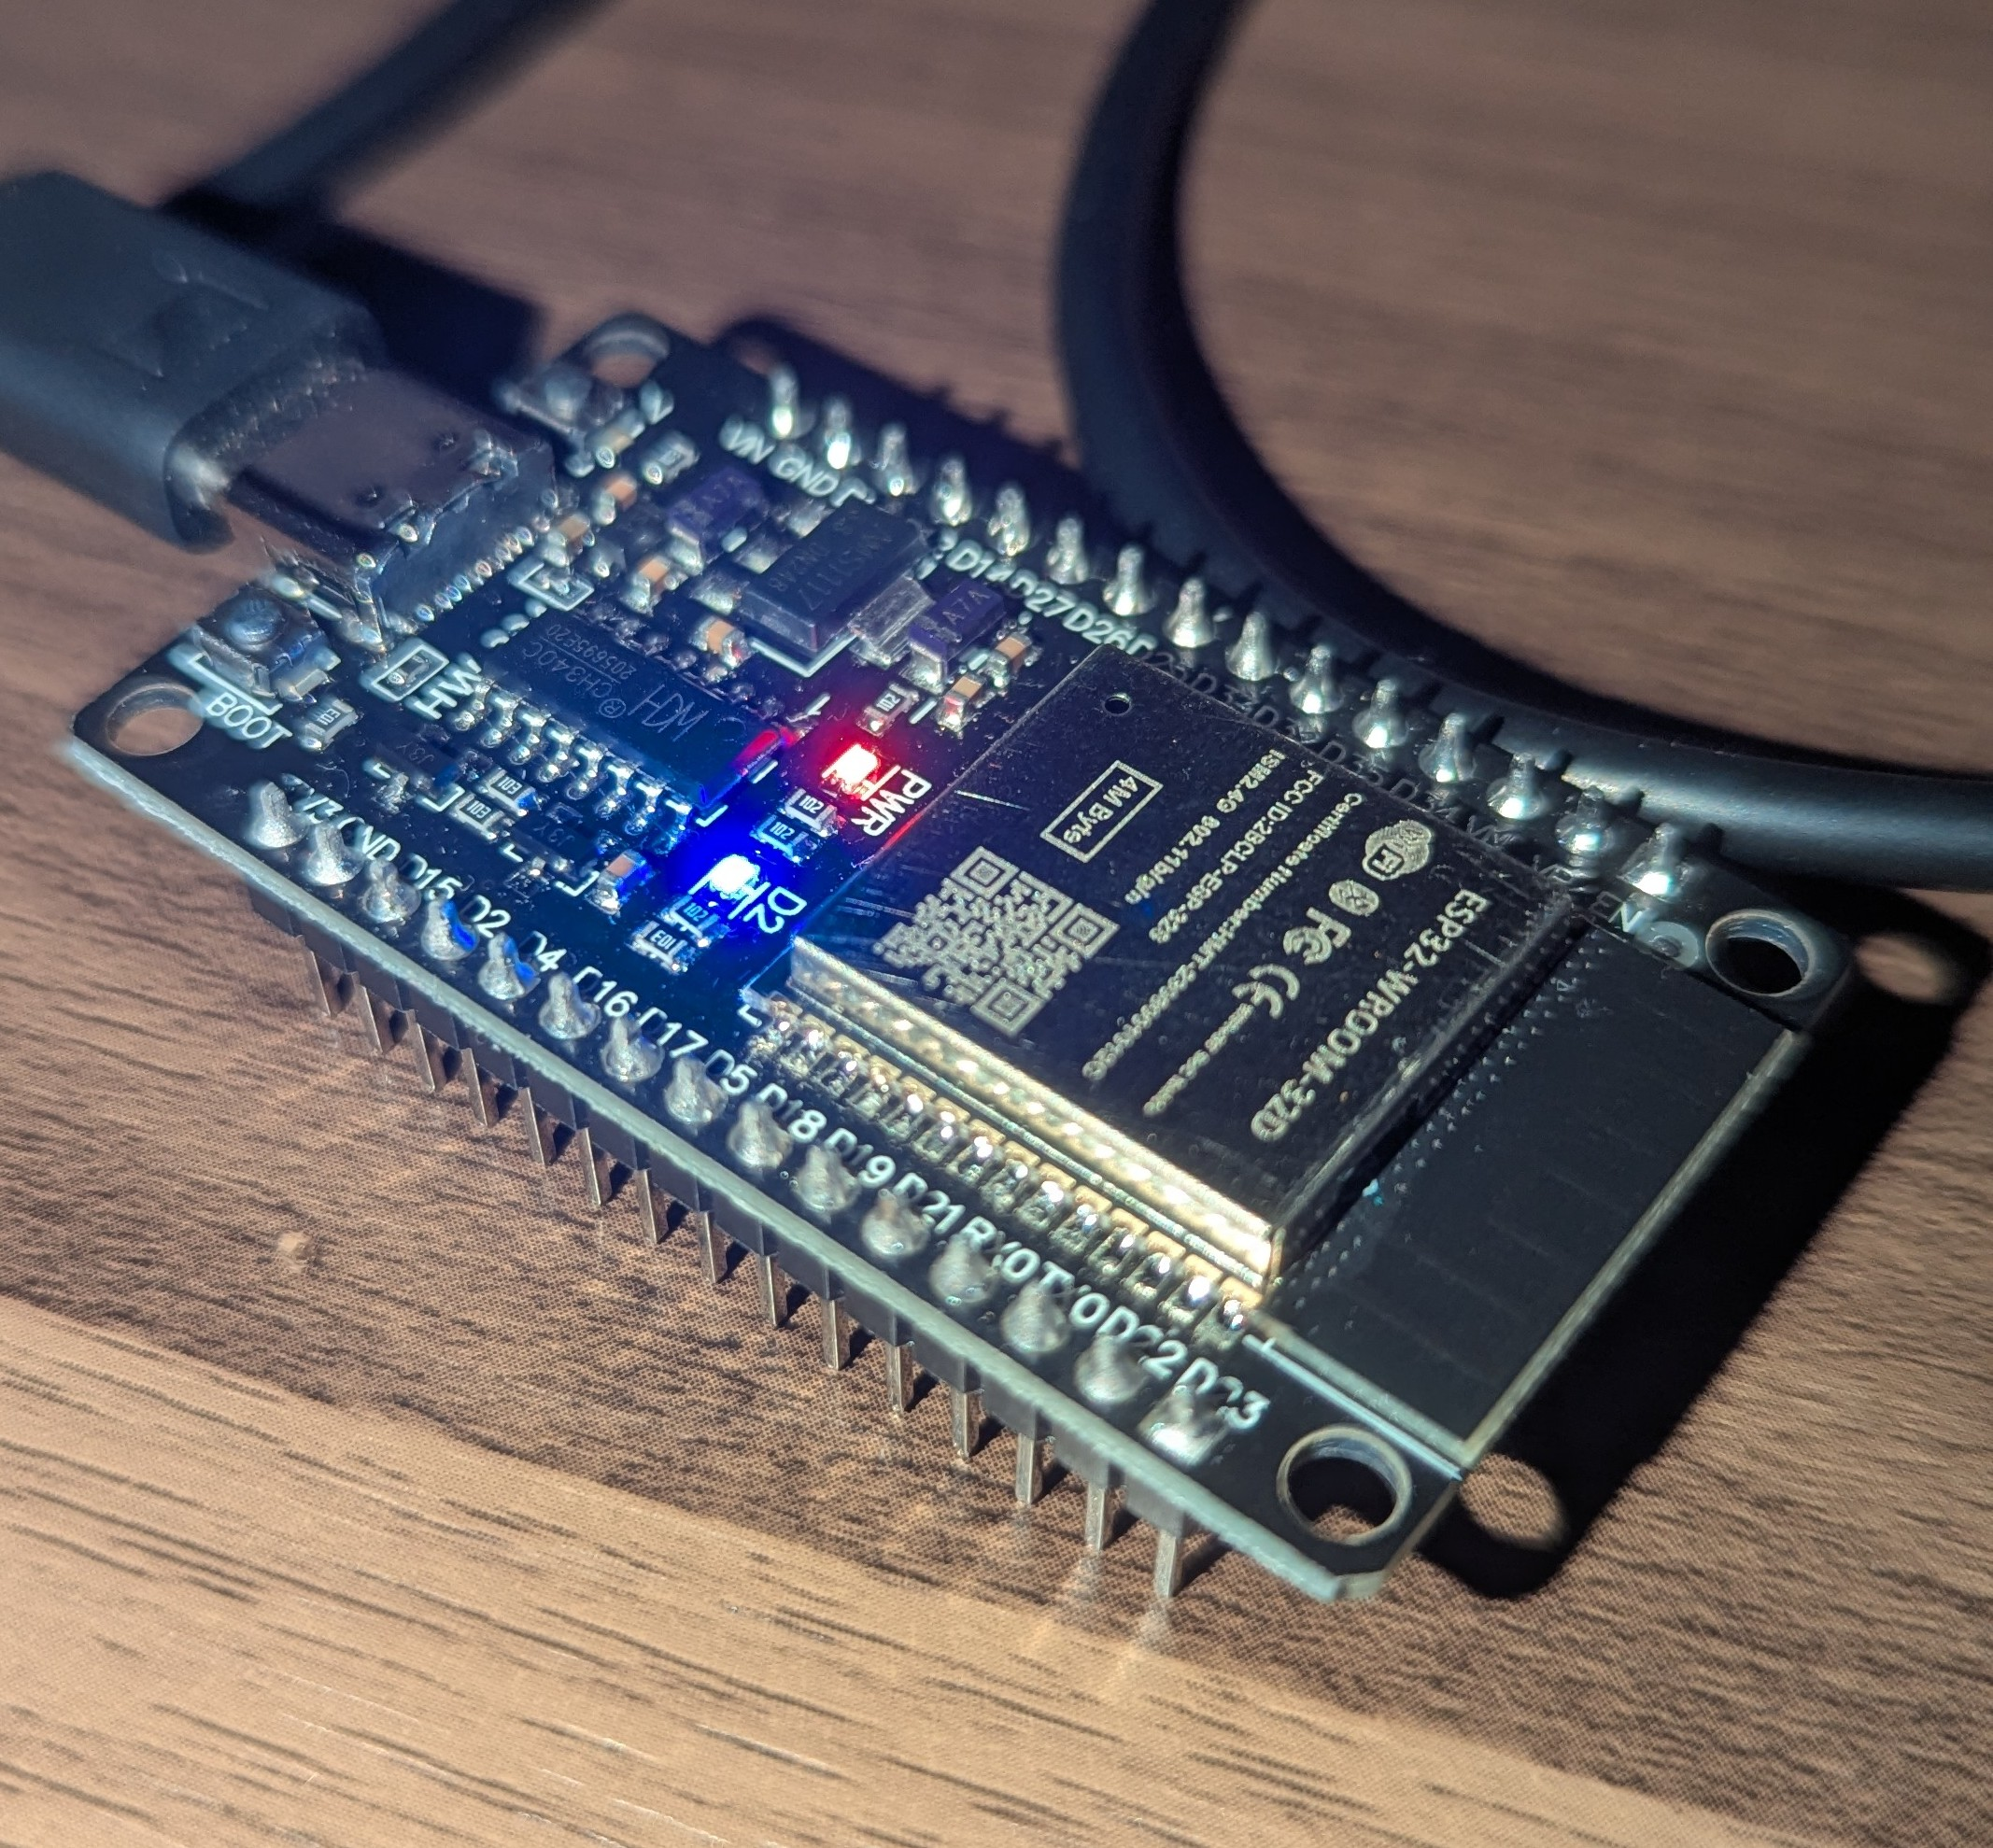
\includegraphics[width=0.5\textwidth, height=0.5\textheight, keepaspectratio]{./img/PXL_20250414_235020869.jpg}
	\caption{Bild eines ESP32 Mikrocontrollers}
	\label{fig:ESP32}
\end{figure}
\newpage

\subsection*{Energiemanagement}
In Heimautomatisierung und IoT-Anwendungen ist \emph{Energiemanagement} zentral, da viele Geräte batteriebetrieben oder dauerhaft aktiv sind. Mikrocontroller bieten verschiedene Low-Power-Modi (z.\,B. Schlafmodus, Tiefschlafmodus), in denen sie unbenötigte Komponenten abschalten oder deren Takt reduzieren, um Energie zu sparen. \autocite{energiesparen} Beispielsweise können Peripherien deaktiviert und durch \emph{Clock Gating} der Takt für inaktive Module angehalten werden, um den Verbrauch zu senken. \autocite{energiesparen} Moderne Techniken wie \emph{Dynamic Voltage and Frequency Scaling} (DVFS) passen zudem Versorgungsspannung und Taktfrequenz dynamisch an die aktuelle Rechenlast an. \autocite{energiesparen} Auf diese Weise lässt sich die Leistungsaufnahme minimieren, ohne die essenziellen Funktionen zu beeinträchtigen. Ein effizientes Energiemanagement verlängert die Batterielaufzeit und reduziert die Wärmeentwicklung – beides essenziell für sensorbasierte Haussteuerungen mit dauerhafter Betriebsbereitschaft.

\subsection*{Echtzeitverhalten}
Eingebettete Systeme zur Steuerung von Geräten im Smart Home unterliegen oft \emph{Echtzeit-Anforderungen}. \emph{Echtzeitsysteme} sind Systeme, die innerhalb vorgegebener Zeitgrenzen korrekt reagieren müssen; das zeitliche Verhalten ist Bestandteil der funktionalen Korrektheit. \autocite{echtzeit_grundlagen} Insbesondere ist die Korrektheit eines Echtzeitsystems nicht nur vom logischen Ergebnis, sondern auch vom physikalischen Zeitpunkt der Ergebniserzeugung bestimmt. \autocite{echtzeit_grundlagen} Man unterscheidet:
\begin{itemize}
  \item \textbf{Harte Echtzeit:} Eine Überschreitung der Deadline führt zu inakzeptablen Folgen (z.\,B. Gefährdung von Personen, Gerätebeschädigung). \autocite{echtzeit_grundlagen}
  \item \textbf{Weiche Echtzeit:} Timing-Verletzungen sind tolerierbar, führen aber zu Leistungseinbußen oder Qualitätsminderungen. \autocite{echtzeit_grundlagen}
\end{itemize}
In der Heimautomatisierung dominieren weiche Echtzeitanforderungen (z.\,B. Heizungsregelung), doch sicherheitsrelevante Funktionen wie Alarmanlagen oder Türschlosssteuerungen erfordern teilweise hartes Echtzeitverhalten. Entsprechend werden Mikrocontroller und ihre Software so ausgelegt, dass deterministische Reaktionszeiten eingehalten werden – etwa durch Einsatz von Echtzeitbetriebssystemen oder direktes Ausführen zeitkritischer Routinen ohne blockierende Aufrufe.

\subsection*{Interrupts}
Zur Realisierung eines responsiven Echtzeitverhaltens verwenden Mikrocontroller sogenannte \emph{Interrupts} (Unterbrechungen). Ein Interrupt ist ein asynchrones Signal, mit dem ein Peripheriegerät oder Sensor den Prozessor veranlasst, das reguläre Programm zu unterbrechen und eine vordefinierte \emph{Interrupt Service Routine (ISR)} auszuführen. Eine häufig zitierte Definition lautet: „Eine asynchrone Unterbrechung (IRQ) ist ein vom Prozessor-externen Umfeld generiertes Signal, das einen Zustand anzeigt und eine Behandlung durch den Prozessor anfordert. Dieses Signal ist nicht mit dem Programmlauf synchronisiert.“ \autocite{echtzeit_grundlagen}
\\
Durch Interrupts können externe Ereignisse (z.\,B. erkannte Bewegung) sofort bearbeitet werden, ohne auf die nächste zyklische Abfrage warten zu müssen. Dies ermöglicht \emph{ereignisgesteuerte Systeme}, die auf externe Signale in quasi Echtzeit reagieren. Alternativ existieren zeitgesteuerte (polling-basierte) Ansätze, bei denen der Mikrocontroller Sensoren in festen Intervallen abfragt. Interruptgesteuerte Designs haben den Vorteil minimaler Latenz, erfordern jedoch sorgfältiges Management (z.\,B. Priorisierung, Interrupt-Latenz), um Abläufe deterministisch und zuverlässig zu halten. In der Praxis werden häufig \emph{kombinierte Ansätze} genutzt: zeitgesteuerte Überwachung für reguläre Aufgaben und Interrupts für dringende Ereignisse.

\subsection*{I/O und Schnittstellen}
Mikrocontroller kommunizieren über diverse \emph{Ein-/Ausgabe-Schnittstellen} mit Sensoren, Aktoren und anderen Systemkomponenten. Sie verfügen über:
\begin{itemize}
  \item \textbf{Digitale I/O-Pins} zur Ansteuerung von Aktoren (z.\,B. Relais für Lampen) oder zum Erfassen binärer Signale (z.\,B. Fensterkontakte).
  \item \textbf{Analoge Eingänge} mit integrierten A/D-Wandlern zur Messung kontinuierlicher Größen (Temperatur, Helligkeit etc.).
  \item \textbf{PWM-Ausgänge} oder D/A-Wandler zur Ansteuerung analoger Aktoren (z.\,B. Dimmsteuerung, Motordrehzahl).
\end{itemize}
Gängige serielle Kommunikationsschnittstellen umfassen:
\begin{itemize}
  \item \textbf{UART (Universal Asynchronous Receiver Transmitter)} – für einfache Punkt-zu-Punkt-Kommunikation (z.\,B. mit Debugger, Bluetooth-Modul),
  \item \textbf{SPI (Serial Peripheral Interface)} – synchroner Hochgeschwindigkeitsbus für kurze Distanzen,
  \item \textbf{I²C (Inter-Integrated Circuit)} – Mehrpunktbus mit Adressierung, ideal für viele Sensorkomponenten,
  \item \textbf{CAN, USB, Ethernet} – für leistungsstärkere Anwendungen, z.\,B. in Gateways oder Fahrzeugtechnik. 
\end{itemize}
\autocite{Microcontroller_vs_Microprocessor}
Viele dieser Schnittstellen sind bereits im Mikrocontroller integriert. \autocite{Microcontroller_vs_Microprocessor} Auch sogenannte \emph{GPIOs} (General Purpose Input/Output) lassen sich flexibel als Ein- oder Ausgang programmieren. Die Vielfalt dieser Schnittstellen erlaubt es einem einzelnen Mikrocontroller, alle für eine Heimautomatisierungsaufgabe relevanten Sensoren und Aktoren direkt anzusteuern, ohne externe Steuerlogik. Die \textbf{korrekte Auswahl und Konfiguration} (z.\,B. Pull-up-Widerstände bei I²C, Bus-Timing, Interruptsteuerung bei UART) ist entscheidend für die Funktionssicherheit des Systems.

\subsection*{Abgrenzung zu System-on-Chips (SoCs)}
Der Begriff \emph{System-on-Chip} (SoC) überschneidet sich funktional mit dem des Mikrocontrollers, bezeichnet jedoch im weiteren Sinne einen integrierten Schaltkreis, der ein vollständiges elektronisches System auf einem Chip vereint. Mikrocontroller können als spezialisierte SoCs betrachtet werden, die primär einen Mikroprozessor mit Speicher und Basisperipherie für Steuerungsaufgaben enthalten.
\\
Im Unterschied dazu integrieren klassische SoCs zusätzliche leistungsfähige Komponenten wie GPU, DSP, drahtlose Kommunikationsmodule (WLAN, LTE), externe Speicheranbindung sowie komplexe Betriebssysteme (z.\,B. Linux, Android). Sie finden sich typischerweise in leistungsfähigen Smart-Home-Zentralen oder Gateways, die Daten aggregieren und komplexe Anwendungen wie Spracherkennung oder Cloud-Anbindung ausführen.
\\
Allgemein gilt: „Ein System-on-Chip ist ein vollständiges elektronisches System auf einem einzigen Chip, der eine Vielzahl von Funktionen ausführen kann.“ Mikrocontroller hingegen sind kompakter, energieeffizienter, günstiger und auf spezifische Aufgaben optimiert. Typische Flash-Größen liegen im Bereich von einigen Kilobyte bis wenigen Megabyte. \autocite{SoC}
\\
\paragraph{Fazit:} In der Heimautomatisierung finden sich beide Technologien: \textbf{Mikrocontroller} in Sensor- und Aktormodulen (z.\,B. ein Feuchtigkeitssensor mit Funkmodul) und \textbf{SoCs} in Smart-Home-Hubs und Gateways, die zentrale Logik und Kommunikation übernehmen.

	\section{Grundlagen des Internet of Things (IoT) und Smart Home}

\subsection{Vernetzte Systeme und Sensorintegration}
Das \emph{Internet of Things} (IoT) bezeichnet ein Netzwerk von physischen Objekten („Dingen“), die mit Sensoren, Software und Konnektivität ausgestattet sind, um Daten zu erfassen und auszutauschen. Im Smart-Home-Kontext bedeutet dies, dass Haushaltsgeräte, Sensoren und Aktoren untereinander sowie mit dem Internet vernetzt sind.
\\
Vernetzte Systeme in der Heimautomatisierung integrieren häufig zahlreiche Sensoren (z.\,B. Temperatur, Bewegung, Luftqualität, Licht, Feuchtigkeit) an verschiedenen Orten des Hauses. Diese übermitteln ihre Daten an zentrale Steuerungen oder Cloud-Dienste. Die Sensorintegration kann sowohl \textbf{lokal} – etwa über ein Heimnetzwerk (WLAN, ZigBee, Z-Wave etc.) an eine Home-Automation-Zentrale – als auch \textbf{cloud-basiert} erfolgen, wobei Sensoren direkt über Internetprotokolle kommunizieren.
\\
Entscheidend ist, dass heterogene Geräte \textbf{interoperabel} kommunizieren können. Smart-Home-Plattformen (z.\,B. Apple HomeKit, Google Home) definieren dazu gemeinsame Protokolle, die eine systemübergreifende Verarbeitung und Steuerung ermöglichen. Neben der Kommunikation ist auch eine lokale \textbf{Datenvorverarbeitung} erforderlich – etwa zum Filtern von Sensorrauschen oder zur Aggregation von Messwerten – um Datenvolumen und Energieverbrauch zu reduzieren.
\\
Die Vernetzung schafft die Grundlage für \textbf{kontextsensitive Entscheidungen} im Smart Home. So kann etwa ein Temperatur- und Feuchtigkeitssensor gemeinsam mit Wetterdaten zur effizienten Heizungsregelung genutzt werden. Insgesamt entsteht ein verteiltes System aus eingebetteten Einheiten, das auf Umweltbedingungen flexibel reagiert. \autocite{IoT}
\\
\subsection{Kommunikationsprotokolle (MQTT, CoAP, HTTP)}
Für die Kommunikation zwischen IoT-Geräten und Diensten haben sich verschiedene spezialisierte Protokolle etabliert:
\\
\paragraph{HTTP (HyperText Transfer Protocol)} 
Das klassische Webprotokoll kommt auch im IoT zum Einsatz – insbesondere bei Geräten, die RESTful-Webservices anbieten. HTTP basiert auf TCP und ist textbasiert, was zu vergleichsweise hohem Overhead führt. Es eignet sich vor allem für leistungsfähige WLAN-Geräte, die direkt mit Cloud-APIs kommunizieren. Vorteile sind die weitverbreitete Infrastruktur und Kompatibilität. Nachteilig sind höhere Latenzen und Energiebedarf. \autocite{IoT_http}
\\
\paragraph{MQTT (Message Queuing Telemetry Transport)} 
MQTT ist ein leichtgewichtiges \textbf{Publish-Subscribe}-Protokoll, das speziell für ressourcenbeschränkte Systeme und instabile Netzwerke entwickelt wurde. Es verwendet TCP als Transportprotokoll und benötigt einen zentralen Broker, der Nachrichten zwischen \emph{Publishern} (z.\,B. Sensoren) und \emph{Subscribern} (z.\,B. Servern oder Aktoren) vermittelt. MQTT zeichnet sich durch minimalen Overhead und Unterstützung für verschiedene \emph{Quality-of-Service}-Stufen aus. Es eignet sich hervorragend für bidirektionale Kommunikation in Echtzeit, z.\,B. zur Steuerung von Lampen oder zur Übermittlung von Messwerten an einen lokalen Broker (z.\,B. Raspberry Pi). \autocite{IoT_mqtt}
\\
\paragraph{CoAP (Constrained Application Protocol)} 
CoAP ist ein binäres, auf UDP basierendes Protokoll für RESTful-Kommunikation unter extrem ressourcenarmen Bedingungen (z.\,B. 6LoWPAN). Es nutzt komprimierte Header, unterstützt optional zuverlässige Übertragungen über Confirmable Messages und erlaubt \textbf{Multicast}. Im Gegensatz zu MQTT ist CoAP stärker auf direkte Client-Server-Interaktionen ausgerichtet und wird häufig in sensornahen IPv6-Netzwerken oder zwischen IoT-Geräten und lokalen Gateways eingesetzt. \autocite{IoT_mqtt}
\\
\paragraph{Zusammenfassung} 
\begin{itemize}[noitemsep]
  \item HTTP: weit verbreitet, aber overheadintensiv – geeignet für leistungsfähige Geräte.
  \item MQTT: effizient für zentrale Nachrichtenvermittlung bei geringen Ressourcen.
  \item CoAP: ideal für direkte, lokale Kommunikation mit geringem Energiebedarf.
\end{itemize}

\noindent Die Protokollwahl beeinflusst maßgeblich Energieeffizienz, Reaktionszeit und Zuverlässigkeit. In modernen Smart-Home-Systemen ist häufig eine Kombination mehrerer Protokolle im Einsatz.
\\
\subsection{Architekturmodelle (Edge, Cloud, Fog)}
Zur effizienten Verteilung von Rechenlast, Speicherbedarf und Steuerlogik im IoT haben sich drei Architekturebenen etabliert:
\\
\paragraph{Edge Computing} 
bezeichnet die Datenverarbeitung direkt am Endgerät, etwa im Mikrocontroller eines Sensors oder Aktors. Vorteilhaft sind minimale Latenz, Ausfallsicherheit bei Verbindungsproblemen und hohe Energieeffizienz. Beispiele sind das lokale Filtern von Sensorwerten oder einfache Steuerentscheidungen (z.\,B. Schwellenwertüberschreitung).
\\
\paragraph{Fog Computing} 
stellt eine mittlere Verarbeitungsebene dar, häufig in Form eines Gateways oder Home-Servers im lokalen Netzwerk. Hier können mehrere Datenströme aggregiert, komplexere Algorithmen ausgeführt oder lokale Regelungen umgesetzt werden. Ein Beispiel ist die Raumtemperaturregelung anhand mehrerer Sensordaten, ohne Cloud-Beteiligung.
\\
\paragraph{Cloud Computing} 
findet in entfernten Rechenzentren statt und bietet skalierbare Ressourcen für Speicherung, Analyse und KI-basierte Optimierung. Typische Aufgaben sind Nutzerverhaltenserkennung, Fernzugriff, Sprachsteuerung, Updates oder Backup-Dienste. Die Cloud erhöht die Funktionalität, ist jedoch auf stabile Internetverbindung angewiesen und bringt höhere Latenzen mit sich.
\\
\paragraph{Hybride Umsetzung} 
In der Praxis arbeiten alle drei Ebenen zusammen: Ein \emph{Edge-Gerät} erkennt z.\,B. eine Türöffnung, der \emph{Fog-Knoten} analysiert das Ereignis und entscheidet über eine Alarmmeldung, während die \emph{Cloud} die Benachrichtigung an das Smartphone des Nutzers übernimmt. Durch diese verteilte Architektur entsteht ein robustes, skalierbares und effizient arbeitendes System. Moderne IoT-Plattformen wie \emph{MEC} (Multi-access Edge Computing) gehen noch einen Schritt weiter, indem sie Cloud-Funktionalitäten näher an das Edge-Gerät verlagern – etwa in den Router oder das Gateway.
\\
\paragraph{Fazit} 
Ein klug verteiltes Architekturmodell erhöht Ausfallsicherheit, reduziert Latenzen und erlaubt eine flexible Skalierung je nach Anwendung und Sicherheitsanforderung. \autocite{edge_fog_cloud} 
\\
\subsection*{Sicherheitsaspekte (Authentifizierung, Datenschutz, Angriffsszenarien)}
Mit zunehmender Vernetzung im Smart Home wachsen die Herausforderungen der IT-Sicherheit und des Datenschutzes. IoT-Geräte sind häufig Ziel von Angriffen, weil sie oft weniger geschützt sind als PCs oder Smartphones. Wichtige Sicherheitsaspekte sind:
\\
\paragraph{Authentifizierung}
Sicherstellen, dass nur berechtigte Benutzer und Geräte Zugriff auf das Smart-Home-System haben. Viele IoT-Geräte werden ab Werk mit Standard-Kennwörtern ausgeliefert, die vom Nutzer selten geändert werden. Dieses bekannte Problem ermöglicht einfache Angriffe: „Viele IoT-Geräte werden mit Standard-Benutzernamen und -Kennwörtern ausgeliefert ... Angreifer kennen diese Standard-Anmeldedaten sehr gut.“ Starke Passwörter oder besser zertifikatsbasierte Authentifizierung sind daher essenziell. Auch Geräte untereinander sollten sich authentisieren (z.\,B. ein Sensor gegenüber dem Gateway), um Spoofing-Angriffe zu verhindern. In modernen Smart-Home-Plattformen kommen oft Public-Key-Verfahren zum Einsatz, bei denen jedes Gerät ein eigenes Schlüsselpaar hat. Fehlende oder schwache Authentifizierung kann dazu führen, dass Angreifer unbefugt Befehle senden (etwa Türöffnung). \autocite{cloudflare}
\\
\paragraph{Datenschutz und Verschlüsselung}
Sensoren im Haus sammeln teils sehr persönliche Daten (Bewegungsprofile, Kameraaufnahmen, Gesundheitsdaten von Wearables etc.). Datenschutz erfordert, dass diese Daten nur zweckgebunden verwendet und angemessen geschützt werden. In der Übertragung ist Verschlüsselung obligatorisch: IoT-Geräte, die unverschlüsselt kommunizieren, ermöglichen Man-in-the-Middle-Angriffe, bei denen ein Angreifer die Daten abfängt und Einblick in das Privatleben erhält. Tatsächlich sind viele IoT-Kommunikationen anfällig, da standardmäßig oft keine Transportverschlüsselung aktiviert ist. Durchgehende Ende-zu-Ende-Verschlüsselung (etwa TLS/DTLS für IP-basierte Protokolle) sollte umgesetzt werden. Zudem müssen in Cloud-Plattformen die Daten gemäß Datenschutzrichtlinien (wie DSGVO) verarbeitet werden – etwa Minimierung der Speicherung personenbeziehbarer Daten oder Anonymisierung von Sensordaten, wo immer möglich. \autocite{cloudflare}
\\
\paragraph{Angriffsszenarien}
IoT-Geräte können auf verschiedene Weise angegriffen werden. Neben Passwort-Angriffen (Brute-Force bekannter Standard-Passwörter) und Abhören unverschlüsselter Verbindungen sind Software-Schwachstellen ein Einfallstor. Viele Smart-Home-Geräte haben unsichere Web-Interfaces oder veraltete Firmware mit bekannten Lücken. Wenn Hersteller keine regelmäßigen Updates/Patches bereitstellen, bleiben diese Lücken offen. Angreifer können so die Kontrolle über Geräte übernehmen und z.\,B. Kameras ausspähen oder das Gerät Teil eines Botnetzes werden lassen.
\\
Ein berühmtes Beispiel ist das \emph{Mirai-Botnet}: eine Malware durchsuchte automatisiert das Internet nach IoT-Geräten mit Standard-Login und infizierte hunderttausende Geräte (vor allem Kameras, Recorder), um daraus ein Botnetz für Distributed-Denial-of-Service (DDoS)-Attacken zu formen. \autocite{proofpoint} „Mirai zielt auf IoT-Geräte ab, bei denen das Standardpasswort noch aktiv ist ... und macht sie zu einem Teil eines Botnets, das dann für einen DDoS-Angriff verwendet wird.“ Dieses Angriffsszenario zeigte eindrücklich, dass auch vermeintlich harmlose Geräte (wie eine vernetzte Kamera) in großer Zahl massive Schäden im Internet anrichten können. \autocite{proofpoint}
\\
\paragraph{Physische Sicherheit}
In Smart Homes stehen IoT-Geräte auch physisch zugänglich in der Wohnung oder sogar außerhalb (Außensensoren, Türklingeln). Ein Angreifer mit physischem Zugriff kann Geräte manipulieren, zurücksetzen oder austauschen. Daher sollten sicherheitskritische Komponenten manipulationsgeschützt installiert werden (z.\,B. Alarm-Zentrale versteckt und sabotagesicher). Zudem sollten Sicherheitschips (Secure Elements) verwendet werden, die kritische Schlüssel speichern, um Hardware-Angriffe zu erschweren.
\\
\paragraph{Angriffsabwehr und Best Practices}
Um das Risiko zu senken, müssen in IoT-Systemen Mechanismen wie Zugriffskontrolle (z.\,B. rollenbasierte Rechte für Nutzer), Sicherheitsprotokolle (z.\,B. regelmäßig wechselnde Tokens, Timeouts für Sessions) und Monitoring (Erkennung ungewöhnlicher Geräteaktivitäten) implementiert werden. Auch im Heimnetz empfiehlt sich Netzwerksegmentierung: IoT-Geräte sollten in ein separates VLAN, um im Falle einer Kompromittierung das Ausbreiten zu verhindern. Nutzeraufklärung spielt ebenfalls eine Rolle – z.\,B. sollte der Bewohner wissen, wie er Geräte sicher einbindet, Updates durchführt und starke Passwörter setzt. 
\\
Sicherheit und Datenschutz sind in der Heimautomatisierung kritische Grundlagen, da die Verletzung dieser Aspekte nicht nur abstrakte IT-Schäden bedeutet, sondern direkt die Privatsphäre und Sicherheit der Bewohner betrifft. Anerkannte Standards und Frameworks (wie \emph{OWASP IoT Top 10} für Gerätesicherheit oder \emph{IEC~62443} für industrielle IoT-Sicherheit) bieten Leitlinien, die zunehmend auch im Consumer-IoT Beachtung finden. Durch \emph{Security by Design} – also Berücksichtigung von Sicherheitsmaßnahmen von der ersten Entwicklungsphase an – sollen zukünftige Smart-Home-Geräte robuste Abwehrmechanismen aufweisen, um das Vertrauen der Nutzer in die Technik zu stärken.

	\section{Regelungstechnik in Software}

\subsection*{Steuerungs- und Regelungskonzepte (Open Loop vs. Closed Loop)}
In eingebetteten Systemen der Heimautomatisierung kommen sowohl Steuerungen (Open-Loop-Control) als auch Regelungen (Closed-Loop-Control) zum Einsatz, je nach Anforderung. Bei einer Steuerung beeinflusst die Software die Stellgr"o\ss en (Aktoren) auf Basis von Eingangsgr"o\ss en nach festgelegter Logik, ohne dass eine R"uckmeldung der Ausgangsgr"o\ss e erfolgt. \autocite{moocit} Das System kennt also den Effekt seiner Eingriffe nicht direkt \textendash{} ein klassisches Beispiel ist eine zeitgesteuerte Gartenbew"asserung: Der Regner schaltet f"ur 10~Minuten ein (Steuerbefehl), unabh"angig davon, ob der Boden schon feucht ist oder nicht.
\\
Eine Regelung dagegen beinhaltet eine R"uckkopplung: Sensoren messen kontinuierlich die Ist-Gr"o\ss e und vergleichen sie mit dem Sollwert; die Software passt die Stellgr"o\ss e laufend an, um Abweichungen auszugleichen. \autocite{haustechnik} Ein Thermostat ist hierf"ur beispielhaft: Die Heizung wird auf Basis der gemessenen Temperatur ein- oder ausgeschaltet, um den Sollwert konstant zu halten. Formal gesprochen: \enquote{Bei einer Regelung wird die Ausgangsgr"o\ss e zur"uckgef"uhrt und mit der F"uhrungsgr"o\ss e (Sollwert) verglichen}, was die Grundlage bildet, um Abweichungen durch Steuerbefehle zu minimieren. \autocite{moocit}
\\
Der Unterschied zwischen offener und geschlossener Wirkungsweise ist wesentlich. Steuerungen (open loop) sind einfach und ben"otigen keine Sensor-R"uckmeldung \textendash{} sie k"onnen jedoch Ungenauigkeiten nicht korrigieren. Regelungen (closed loop) sind aufwendiger (erfordern Sensorik und Regleralgorithmen), bieten aber Genauigkeit und Robustheit gegen"uber St"orungen.
\\
In der Praxis verwendet man in Smart Homes h"aufig Regelungen "uberall dort, wo Pr"azision wichtig ist (z.,B. Temperaturregelung, Motordrehzahlregelung in Rolll"aden), w"ahrend reine Steuerungen f"ur simpler gelagerte Aufgaben oder als Sicherheitsebene eingesetzt werden. Oft gibt es auch Kombinationen: etwa eine Zeitsteuerung mit einer nachgeschalteten Regelung. Die Beherrschung dieser Konzepte setzt Kenntnisse in der Regelungstechnik voraus, also mathematische Beschreibung von Regelkreisen, Stabilit"atskriterien etc., was in die Software implementiert wird.
\\
\subsection*{Schwellenwertsteuerung}
Eine einfache Form der Regelung/Steuerung ist die Schwellenwertsteuerung, oft auch Zwei-Punkt-Regelung genannt. Hierbei wird eine Aktion ausgel"ost, sobald eine Messgr"o\ss e einen definierten Schwellenwert "uber- oder unterschreitet. Das System kennt also nur zwei Zust"ande \textendash{} z.B. Heizung \textbf{EIN} vs. \textbf{AUS} abh"angig davon, ob die Temperatur unter oder "uber dem Sollwert liegt.
\\
Ein klassisches Beispiel ist der einfache Thermostat: F"allt die Raumtemperatur unter 20~\textdegree{}C, schaltet der Regler die Heizung an; steigt sie "uber 20~\textdegree{}C, wird die Heizung abgeschaltet. \autocite{haustechnik}
\\
Solche Schwellenwertsteuerungen arbeiten diskontinuierlich (die Stellgr"o\ss e springt zwischen zwei Werten) und sind leicht implementierbar (\texttt{if-then}-Logik in Software). Vorteil ist die Einfachheit und oft hohe Zuverl"assigkeit; Nachteil k"onnen Schwingungen oder st"andiges Ein/Aus-Schalten sein, wenn keine Hysterese eingebaut ist. Daher f"ugt man praktisch meist eine Hysterese hinzu \textendash{} z.B. Heizung \textbf{an} unter 19,5~\textdegree{}C und erst \textbf{aus} "uber 20,5~\textdegree{}C \textendash{} um ein zu h"aufiges Schalten zu vermeiden.
\\
In vielen Heimautomatisierungs-Szenarien gen"ugt eine Schwellenwertsteuerung: etwa das Einschalten des Lichts bei Unterschreiten eines Helligkeitswerts, "Offnen der Jalousie bei "Uberschreiten eines Helligkeitsgrenzwerts oder L"uften bei "Uberschreiten eines CO\textsubscript{2}-Schwel\-len\-werts. Die Implementierung erfolgt in der Software meist durch Abfragen der Sensorsignale und Setzen der Aktorausg"ange entsprechend der festgelegten Grenzwerte.
\\
Diese Form der Steuerung z"ahlt zu den unstetigen Reglern (bin"are Ausgangszust"ande) und kann als Sonderfall einer Regelung angesehen werden (der Istwert wird mit dem Grenzwert verglichen = R"uckf"uhrung vorhanden, aber Stellgr"o\ss e nimmt nur zwei Zust"ande an). Insbesondere in sicherheitsgerichteten Funktionen (z.,B. Gasmelder \textendash{} Gas "uber Schwelle $\Rightarrow$ Ventil zu) sind Schwellenwertmechanismen beliebt wegen ihrer Klarheit und Nachvollziehbarkeit.
\\
\subsection*{Einfache Regler (P, PI, PID)}
F"ur feinere Kontrolle kontinuierlicher Gr"o\ss en werden in der Regelungstechnik h"aufig lineare Regler eingesetzt, vor allem die Familien der \textbf{P}-, \textbf{PI}-, \textbf{PD}- und \textbf{PID}-Regler. Diese sind durch die drei Grundaktionen \emph{Proportional (P)}, \emph{Integral (I)} und \emph{Differential (D)} gekennzeichnet, die auch kombiniert auftreten k"onnen.
\\
In eingebetteten Steuerungen eines Smart Homes findet man z.,B. in Heizungs- oder Klimaregelungen oft \textbf{PI-Regler}, um eine konstante Temperatur ohne bleibenden Fehler einzuregeln, oder \textbf{PID-Regler} in Motorsteuerungen (z.,B. f"ur L"ufter oder Pumpen), um schnelle und stabile Stellgr"o\ss enregelungen zu erreichen.
\\
\paragraph{P-Regler (Proportionalregler):} Die Stellgr"o\ss e wird proportional zur aktuellen Regelabweichung \[
e(t) = \mathrm{Soll} - \mathrm{Ist}
\]
\\
 ver"andert. Der P-Anteil reagiert damit sofort auf Abweichungen \textendash{} je gr"o\ss er der Fehler, desto st"arker das Stellsignal. Dadurch wird ein direktes Korrekturverhalten erzielt: Ist die Raumtemperatur 2~\textdegree{}C unter dem Sollwert, erh"oht ein P-Regler z.,B. das Ventil "uberproportional.
 \\
Allerdings f"uhrt ein reiner P-Regler meist zu einer bleibenden Regeldifferenz (Offset), da er bei Erreichen des Sollwerts das Stellsignal auf null reduziert, noch bevor der Istwert exakt den Sollwert erreicht.

\paragraph{I-Regler (Integralregler):} Der I-Anteil integriert die vergangene Regelabweichung \textendash{} Fehler werden "uber die Zeit aufaddiert. Dies erm"oglicht es, einen bleibenden Fehler auszugleichen. \autocite{steuern_regeln} Der I-Anteil reagiert langsam, ist aber in PI/PID-Reglern essenziell, um den station"aren Fehler zu beseitigen.

\paragraph{D-Regler (Differenzialregler):} Der D-Anteil ber"ucksichtigt die "Anderungsgeschwindigkeit der Regelabweichung, also $de(t)/dt$. Er wirkt d"ampfend auf schnelle "Anderungen und reduziert "Uberschwingen. \autocite{steuern_regeln} In Software wird er meist durch Differenzen zwischen zwei Abtastzeitpunkten gen"ahert.

\paragraph{PI- und PID-Regler:} Kombinationen dieser Typen (PI, PID) vereinen schnelles Reagieren (P), Fehlerausgleich (I) und D"ampfung (D). Ein PID-Regler bietet geringe Einschwingzeit, keine bleibende Regelabweichung und gutes St"orverhalten. In der Software wird ein PID-Regler meist diskret realisiert, z.,B. mit:
\begin{equation}
u(t) = K_P \left( e(t) + \frac{1}{T_I} \int e(t) dt + T_D \frac{de(t)}{dt} \right)
\end{equation}
\autocite{steuern_regeln_2}
\subsection*{Datenverarbeitung zur Entscheidungsfindung}
Vor jeder Stellentscheidung muss das System die Rohdaten aufbereiten. Dazu z"ahlen:
\begin{itemize}
\item \textbf{Signalaufbereitung:} Rauschfilterung, Mittelwertbildung, Kalibrierung.
\item \textbf{Sensorfusion:} Zusammenf"uhren mehrerer Quellen zur robusteren Entscheidungsbasis.
\item \textbf{Zustandsautomaten:} Logiksteuerung je nach Betriebsmodus.
\item \textbf{KI-gest"utzte Algorithmen:} Zunehmender Einsatz von Embedded AI zur Prognose und Mustererkennung.
\item \textbf{Fehlererkennung:} Erkennen fehlerhafter oder ausgefallener Sensoren und Wechsel in Failsafe-Zust"ande.
\end{itemize}

\noindent Nach dieser Verarbeitung wird auf Basis der Sensordaten entschieden, ob eine Steuerung oder Regelung aktiviert wird. Die Datenverarbeitung bildet somit die Br"ucke zwischen physikalischer Messung und softwarebasierter Aktorik. Sie ist damit essentiell f"ur eine sichere, pr"azise und energieeffiziente Heimautomatisierung.



	\newpage
	
	\chapter{Anforderungen}
        \section{Reflexion zur Frontend-Umsetzung}

Die Umsetzung des Frontends im Rahmen dieses Projekts kann insgesamt als gelungen und stabil bewertet werden. Die Anwendung ist vollständig funktionsfähig und unterstützt sowohl die deutsche als auch die englische Sprache durch ein konsistentes Internationalisierungskonzept. Zusätzlich bietet das Interface die Auswahl zwischen einem Dark Mode und einem Light Mode, was zur Barrierefreiheit und zum Nutzungskomfort beiträgt.

Besonders hervorzuheben ist das moderne, einheitliche und visuell ansprechende Design, das konsequent auf aktuellen UI/UX-Prinzipien basiert. Durch die Integration von Gamification-Elementen wie individuellen Pflanzen-Avataren wurde die Nutzerbindung zusätzlich gestärkt. Die Verwendung bewährter Best Practices in der Frontend-Architektur sowie die Orientierung am Flux-Prinzip sorgen für einen klar strukturierten Datenfluss und eine effiziente Benutzerinteraktion.

Ein wesentlicher Aspekt der Frontend-Gestaltung war die Gewährleistung eines flüssigen Nutzererlebnisses durch intuitive Navigation und konsistente Layouts. Die modular aufgebaute Komponentenstruktur ermöglicht eine gute Wartbarkeit und einfache Erweiterbarkeit der Anwendung.

\subsection{Verbesserungspotential}

Trotz der grundsätzlich hohen Qualität bestehen einige Optimierungsmöglichkeiten. Zum einen könnten Performance-Verbesserungen vorgenommen werden, um die Ladezeiten insbesondere bei datenintensiven Ansichten zu verringern. Zum anderen wurden einige Zusatzfunktionen aus zeitlichen Gründen nicht realisiert, die in einer späteren Entwicklungsphase ergänzt werden können.

Darüber hinaus sind drei kleinere Bugs bekannt, die zum aktuellen Stand noch nicht behoben wurden:

\begin{itemize}
	\item Auf Geräten ab der Android API Version 35 kann es bei aktivierter Drei-Punkte-Navigationsleiste zu einer Überlappung mit der App-eigenen Navigationsleiste kommen.
	\item Nach der Erstellung einer neuen Gruppe werden die darin enthaltenen Räume in der Bearbeitungsansicht nicht sofort angezeigt, sofern kein Seitenwechsel oder manueller Refresh erfolgt.
    \item Man bekommt einen Fehler, wenn man eine Pflanze bearbeitet, die einen fremden Controller hat, weil im Backend diese Änderungen nicht angenommen werde.
\end{itemize}

Diese Einschränkungen haben jedoch keinen kritischen Einfluss auf die Hauptfunktionen und Nutzbarkeit der Anwendung.

Bei einer Weiter Entwicklung des Frontends und damit auch bei einer realen Nutzung sollten Frontend-Test in Verbindung mit E2E-Tests durchgeführt werden. Dadurch können Funktionen überprüft und Bugs vermieden werden. 

\subsection{Fazit}

Die in der Konzeption formulierten Anforderungen an das Frontend wurden weitestgehend erfolgreich umgesetzt. Die Anwendung bietet ein modernes, benutzerfreundliches Interface mit internationaler Ausrichtung und ansprechendem Design. Funktionalität, Nutzerfluss und Wartbarkeit konnten auf hohem Niveau realisiert werden. Die identifizierten Verbesserungspunkte bieten darüber hinaus eine wertvolle Grundlage für zukünftige Weiterentwicklungen.

        Für das Projekt Sensora gelten hohe Anforderungen an Zuverlässigkeit, Sicherheit, Erweiterbarkeit und Datenintegrität. In diesem Kapitel werden die formellen Anforderungen an das Backend sowie an die zugrunde liegende Datenbankarchitektur getrennt voneinander dargestellt. Ziel ist es, eine tragfähige Grundlage für die technische Umsetzung zu schaffen.
        \section{Anforderungen an die entwickelten Schnittstellen-Services im Projekt Sensora}

Die Hauptaufgabe der Schnittstellen-Services lag in der Konzeption und Realisierung mehrerer Dienste, die als Vermittlungskomponenten zwischen Sensor-Controllern, Benutzerschnittstellen, dem zentralen Datenspeicher sowie einem Nachrichtenübertragungsmechanismus fungieren. Diese Services sind nicht Bestandteil der Steuerlogik auf Hardwareebene, sondern unterstützen den bidirektionalen Informationsaustausch und die sichere Verwaltung verteilter Geräteinstanzen.

Ziel dieses Kapitels ist es, die funktionalen und nicht-funktionalen Anforderungen an diese Schnittstellenkomponenten technologieoffen zu definieren. Die konkrete Wahl der eingesetzten Technologien sowie deren theoretische Fundierung erfolgt erst in den nachfolgenden Kapiteln.

\subsection{Allgemeine Anforderungen an alle Schnittstellen-Services}

Unabhängig von ihrer konkreten Aufgabe müssen sämtliche entwickelten Services folgende generelle Anforderungen erfüllen, die sich aus dem Aufbau des Gesamtsystems sowie den Entwicklungsprinzipien eines modernen verteilten Softwaresystems ergeben:

\begin{itemize}
  \item \textbf{Modularität:} Die Komponenten sollen entkoppelt und unabhängig voneinander betreibbar sein, sodass sie einzeln aktualisiert, getestet und ersetzt werden können.

  \item \textbf{Plattformunabhängigkeit:} Die Services müssen innerhalb einer containerisierten Umgebung lauffähig sein und dürfen keine plattformspezifischen Abhängigkeiten voraussetzen.

  \item \textbf{Fehlertoleranz:} Die Komponenten müssen so gestaltet sein, dass bei Ausfall abhängiger Systeme (z.\,B. Netzwerk, Datenbank) keine kritischen Fehler entstehen. Entsprechende Retry-Mechanismen und Fehlerprotokollierung sind vorzusehen.

  \item \textbf{Datensicherheit:} Sensible Informationen dürfen zu keinem Zeitpunkt im Klartext übertragen oder ungeschützt gespeichert werden. Eine sichere Authentifizierung und Zugriffsbeschränkung ist auf allen öffentlich erreichbaren Schnittstellen erforderlich.

  \item \textbf{Skalierbarkeit und Erweiterbarkeit:} Die Architektur der Services soll so beschaffen sein, dass zusätzliche Sensoren, Controller oder Benutzer ohne grundlegende Systemänderungen hinzugefügt werden können.

  \item \textbf{Zuverlässigkeit bei der Kommunikation:} Die Kommunikation zwischen Services sowie mit externen Geräten soll gegen Nachrichtenverlust abgesichert sein, insbesondere bei systemkritischen Operationen wie Steuerbefehlen oder Datenspeicherung.
\end{itemize}

\section{Anforderungsanalyse für die entwickelten Services}

Im Folgenden werden die spezifischen Anforderungen an die einzelnen Services beschrieben, wobei sowohl funktionale Anforderungen (Was soll der Service leisten?) als auch systemische Rahmenbedingungen betrachtet werden.

\subsection{Registrierungs- und Authentifizierungsservice (Auth-Service)}

Der Auth-Service bildet die sicherheitsrelevante Schnittstelle zur Einbindung verteilter Steuergeräte (Controller) in das System. Er ist verantwortlich für die Validierung, Registrierung und individuelle Konfiguration dieser Geräte.

\subsubsection{Funktionale Anforderungen}
\begin{itemize}
  \item Der Service muss es ermöglichen, neue Geräteinstanzen kontrolliert durch autorisierte Verwaltungsprozesse zu registrieren. Eine unbeaufsichtigte Selbstregistrierung ist auszuschließen.
  
  \item Für jede registrierte Geräteinstanz ist ein eindeutiger Identifikator sowie ein zugehöriges Zugriffsprofil zu erzeugen. Dieses Profil muss zur differenzierten Rechtevergabe geeignet sein.
  
  \item Die Authentifizierung eines Geräts gegenüber dem System muss über ein sicheres Verfahren erfolgen, das keine langfristige Speicherung von Klartextgeheimnissen erfordert und gleichzeitig eine manipulationssichere Verifikation ermöglicht.

  \item Nach erfolgreicher Authentifizierung soll eine Kommunikationsfähigkeit zwischen Gerät und System ermöglicht werden, die sich explizit auf festgelegte Kommunikationskanäle beschränkt.

  \item Der Service muss relevante Metadaten persistieren, sodass die zugehörige Gerätelogik (z.\,B. Sensor- oder Aktorzuordnung) systemweit nachvollzogen werden kann.
\end{itemize}

\subsubsection{Nicht-funktionale Anforderungen}
\begin{itemize}
  \item Die Registrierungslogik darf nur durch explizit autorisierte Systeme oder Nutzer aufrufbar sein.
  \item Die Kommunikation mit dem Service muss verschlüsselt erfolgen.
  \item Eine versehentliche Mehrfachregistrierung desselben Geräts ist zu erkennen und abzuweisen.
\end{itemize}

\subsection{E-Mail-Verifikationsservice (Mail-Service)}

Der Mail-Service übernimmt die Kommunikation mit Nutzenden zur Verifizierung neu angelegter Benutzerkonten. Seine primäre Aufgabe ist es, die Zustellung von zeitlich begrenzten Bestätigungslinks zu ermöglichen.

\subsubsection{Funktionale Anforderungen}
\begin{itemize}
  \item Der Service muss über eine Schnittstelle ansprechbar sein, über die Verifizierungsanfragen gestellt werden können.
  \item Nach Validierung der Anfrage ist ein einmalig nutzbarer Link zu generieren und über einen gängigen E-Mail-Dienst an den Empfänger zu übermitteln.
  \item Bei Aufruf des Verifikationslinks muss der Status des entsprechenden Benutzerkontos im System aktualisiert werden.
\end{itemize}

\subsubsection{Nicht-funktionale Anforderungen}
\begin{itemize}
  \item Nur autorisierte Systeme dürfen Anfragen zur Mailverifikation stellen.
  \item Die Verifizierung darf nur erfolgen, wenn die Kombination aus Benutzername und E-Mail-Adresse im System bekannt ist.
  \item Ein nicht eingelöster Verifizierungslink muss nach Ablauf einer definierten Zeitspanne seine Gültigkeit verlieren.
\end{itemize}

\subsection{Datenschreibdienst für Messdaten (Database Writer)}

Dieser Dienst verarbeitet eingehende Datenströme von Sensoren und persistiert die extrahierten Informationen strukturiert in einem relationalen Datensystem.

\subsubsection{Funktionale Anforderungen}
\begin{itemize}
  \item Der Dienst muss kontinuierlich eingehende Daten von Messgeräten empfangen, analysieren und in geeigneter Form speichern.
  \item Die Identität der messenden Einheit muss eindeutig ermittelbar sein. Ist die Einheit im System nicht bekannt, so muss diese bei Bedarf dynamisch registriert werden können.
  \item Die Speicherung darf nur erfolgen, wenn eine vollständige logische Zuordnung der Sensordaten zu einer Pflanze bzw. zum zugehörigen Anwendungsfall gegeben ist.
  \item Es müssen regelmäßig alle bekannten Sensoren auf Aktivität geprüft werden. Wird über einen definierten Zeitraum keine neue Messung empfangen, ist dies systemintern als Fehlverhalten zu markieren.
\end{itemize}

\subsubsection{Nicht-funktionale Anforderungen}
\begin{itemize}
  \item Der Dienst muss bei Netzwerkausfällen oder vorübergehenden Störungen in der Verbindung zur Datenbank stabil bleiben.
  \item Wiederholte Nachrichtenübertragungen dürfen nicht zu doppelten Datensätzen führen.
  \item Die Datenverarbeitung muss nachvollziehbar protokolliert werden, um Fehler oder Auffälligkeiten zu diagnostizieren.
\end{itemize}

\subsection{Service zur Steuerung von Zielwerten (Setpoint API)}

Über diesen Dienst können Zielwerte (Sollwerte) für bestimmte Sensoren oder Aktoren von außen gesetzt werden. Ziel ist es, die Regelgrößen im System dynamisch anpassen zu können.

\subsubsection{Funktionale Anforderungen}
\begin{itemize}
  \item Der Dienst muss eine externe Schnittstelle bereitstellen, über die Zielwerte für bestimmte Komponenten adressiert werden können.
  \item Der Dienst muss in der Lage sein, die übermittelten Steuerinformationen an die richtige Geräteinstanz weiterzuleiten.
  \item Die übertragenen Datenpakete müssen die Zuordnung zur Zielkomponente sowie den anvisierten Wert enthalten.
  \item Eine Dokumentation der Schnittstelle muss vorliegen, um die Integration in andere Komponenten zu ermöglichen.
\end{itemize}

\subsubsection{Nicht-funktionale Anforderungen}
\begin{itemize}
  \item Der Dienst darf keine gespeicherten Zustände über Zielwerte vorhalten.
  \item Die Kommunikation muss so gestaltet sein, dass sie eine zuverlässige Zustellung ermöglicht.
  \item Fehlkonfigurationen oder fehlerhafte Eingaben müssen zu validierbaren Fehlermeldungen führen.
\end{itemize}

\subsection{Konfigurationsdienst für Kommunikationsinfrastruktur (Solace Init)}

Dieser Service ist verantwortlich für die initiale Einrichtung der Kommunikationsinfrastruktur im System, insbesondere im Hinblick auf Messaging-Komponenten wie Queues oder themenbasierte Weiterleitungspfade.

\subsubsection{Funktionale Anforderungen}
\begin{itemize}
  \item Der Dienst muss eine maschinenlesbare Konfiguration interpretieren können, in der Kommunikationskanäle, Routingregeln und Zugriffspfade definiert sind.
  \item Auf Basis dieser Konfiguration muss die zugrunde liegende Infrastruktur um definierte Ressourcen ergänzt werden.
  \item Bereits existierende Konfigurationselemente dürfen dabei nicht überschrieben oder dupliziert werden.
\end{itemize}

\subsubsection{Nicht-funktionale Anforderungen}
\begin{itemize}
  \item Der Dienst muss so gestaltet sein, dass er mehrfach ausgeführt werden kann, ohne die Konsistenz der Kommunikationsstruktur zu gefährden.
  \item Fehlerhafte Konfigurationseinträge sind zu erkennen, protokollieren und dürfen die Verarbeitung nicht abbrechen.
\end{itemize}

        \section{Anforderungen an das Backend}
Das Backend bildet die zentrale Kommunikationsschnittstelle zwischen Clients, internen Services und der Datenbank. Entsprechend hoch sind die Anforderungen an Struktur, Sicherheit und Stabilität.

\subsection{Architektur und Technologien}
\begin{itemize}
    \item Das Backend ist als \ac{rest}-Service zu implementieren.
    \item Es muss eine modulare, wartbare Architektur aufweisen, die dem Prinzip der Trennung von Zuständigkeiten (Separation of Concerns) folgt.
    \item Als Technologie-Stack wird eine moderne, performante Sprache wie Rust mit einem Webframework wie actix\_web empfohlen.
\end{itemize}

\subsection{Authentifizierung und Autorisierung}
\begin{itemize}
    \item Alle Zugriffe auf geschützte Ressourcen müssen durch ein Authentifizierungsverfahren abgesichert werden (z.B. \ac{jwt} oder OAuth2).
    \item Autorisierungen auf Zeit wie z.B. Sessions sind nicht erlaubt. Alternativen zu Passwörtern (z.B. Tokens) müssen begrenzt gültig sein.
\end{itemize}

\subsection{Fehlerbehandlung und Logging}
\begin{itemize}
    \item Fehlerzustände müssen konsistent behandelt und in einem strukturierten Format an den Client kommuniziert werden.
    \item Es ist ein mehrstufiges Logging-System zu implementieren, das zwischen Info, Warnung und Fehler unterscheidet.
    \item Sensible Informationen dürfen in Logs nicht gespeichert werden. Logs müssen zentral gesammelt und gegen Manipulation abgesichert werden.
\end{itemize}

\subsection{Skalierbarkeit und Performance}
\begin{itemize}
    \item Das Backend ist zustandslos zu gestalten, um horizontale Skalierung über Load-Balancing zu ermöglichen.
    \item Die Antwortzeiten für einfache \ac{crud} Operationen sollen im Normalbetrieb unter 100ms liegen.
    \item Die Architektur soll auf Lastspitzen vorbereitet sein (z.B. durch Queues oder Caching).
\end{itemize}

\subsection{Sicherheit}
\begin{itemize}
    \item Gängige Sicherheitslücken (z.B. SQL-Injection, XSS, CSRF) sind durch geeignete Mechanismen zu verhindern.
    \item Eingaben vom Client sind streng zu validieren und zu sanitieren.
\end{itemize}

\subsection{API-Dokumentation}
\begin{itemize}
    \item Die Schnittstellen müssen vollständig dokumentiert werden.
    \item Eine maschinenlesbare API-Spezifikation (z.B. OpenAPI 3.0) ist zu pflegen.
    \item Optional kann eine interaktive API-Oberfläche für Entwickler bereitgestellt werden (z.B. Swagger UI).
\end{itemize}

\section{Anforderungen an die Datenbank}
Die Datenbank dient als persistente Grundlage für alle im System gespeicherten Informationen. Sie muss sowohl performant als auch sicher und konsistent arbeiten.

\subsection{Modellierung und Struktur}
\begin{itemize}
    \item Das Datenbankschema ist klar zu dokumentieren und mindestens in der 3. Normalform zu entwerfen, sofern nicht durch Performance-Aspekte begründet anders.
    \item Entitäten und ihre Beziehungen müssen nachvollziehbar und versionierbar abgebildet werden.
\end{itemize}

\subsection{Datensicherheit und Integrität}
\begin{itemize}
    \item Sensible Daten (z.B. Passwörter, Tokens) müssen verschlüsselt gespeichert werden.
    \item Datenbankeigene Mechanismen wie Constraints, Foreign Keys und ggf. Trigger sind zur Sicherstellung der Datenintegrität zu verwenden.
    \item Referentielle Integrität ist in allen relevanten Tabellen durchzusetzen.
\end{itemize}

\subsection{Zugriffskontrolle}
\begin{itemize}
    \item Der Datenbankzugriff erfolgt ausschließlich über definierte Rollen mit minimalen Rechten.
    \item Es muss zwischen Administrations-, Lese- und Schreibzugriff differenziert werden.
    \item Externe Dienste erhalten nur selektiven Zugriff auf erforderliche Tabellen.
\end{itemize}

\subsection{Backups und Wiederherstellung}
\begin{itemize}
    \item Es ist ein automatisiertes Backup-Konzept zu implementieren, welches tägliche Snapshots sowie inkrementelle Sicherungen vorsieht.
    \item Wiederherstellungsroutinen müssen dokumentiert und regelmäßig geprüft werden.
\end{itemize}

\subsection{Performance und Skalierung}
\begin{itemize}
    \item Für häufig genutzte Felder sind geeignete Indizes zu definieren.
    \item Bei wachsendem Datenvolumen sollen Mechanismen wie Read-Replicas, Sharding oder Partitionierung zum Einsatz kommen.
    \item Abfragen müssen gezielt optimiert und auf lange Laufzeiten geprüft werden.
\end{itemize}

\subsection{Technologischer Rahmen}
\begin{itemize}
    \item Die Datenbanklösung muss Open Source, stabil, transaktionssicher und für hohe Datenmengen geeignet sein.
    \item Es wird der Einsatz von PostgreSQL empfohlen.
\end{itemize}
        \section{Anforderungen an das IoT-Gerät}
\label{sec:Anforderungen_IoT}
\subsection{Allgemeine Anforderungen an das IoT-Gerät}

Das IoT-Gerät fungiert als zentrale Steuerkomponente innerhalb des automatisierten Bewässerungssystems. Es ist zuständig für die zyklische Erfassung und Verarbeitung von Umweltdaten, die Aktorsteuerung basierend auf festgelegten Zielparametern sowie die gesicherte Kommunikation mit externen Systemen. Neben diesen Kernfunktionen umfasst seine Verantwortung auch die Konfigurierbarkeit des Systems, die Benutzerinteraktion bei der Erstinbetriebnahme und die Ausgabe von Statusinformationen.
\\
Zur Erfüllung dieser Aufgaben muss das IoT-Gerät eine Vielzahl unterschiedlicher Anforderungen erfüllen, die sowohl funktionale als auch nicht-funktionale Aspekte abdecken. Diese Anforderungen werden im Folgenden detailliert analysiert.

\subsection{Anforderungsanalyse für das IoT-Gerät}

\subsubsection{Integration und zyklische Abfrage von Sensorik}

Das System muss in der Lage sein, Umweltdaten über mehrere physikalisch unterschiedliche Sensoren zu erfassen. Dabei kommen sowohl analoge Signale (z.\,B. Bodenfeuchtesensor) als auch digitale Schnittstellen (z.\,B. I²C für Lichtsensor und GPIO für Temperatur- und Feuchtesensoren) zum Einsatz. Die Erfassung erfolgt in regelmäßigen Intervallen durch zyklische Tasks.
\\
Eine besondere Anforderung besteht darin, dass jeder Sensor vor seiner Nutzung initialisiert und zyklisch auf Funktionsfähigkeit überprüft wird. Das System muss erkennen, ob ein Sensor inaktiv ist – etwa durch konstanten Maximalwert oder fehlende Signale – und diesen entsprechend markieren. Dadurch wird verhindert, dass fehlerhafte Sensordaten zu Fehlentscheidungen im Steuerungssystem führen.

\subsubsection{Messdatenverarbeitung, Validierung und Zeitstempelung}

Die erfassten Rohdaten müssen einer mehrstufigen Verarbeitung unterzogen werden, um zuverlässige, regelbare Kenngrößen zu erhalten. Dabei sind insbesondere folgende Prozesse umzusetzen:

\begin{itemize}
	\item \textbf{Mittelwertbildung:} Zur Reduktion von Ausreißern wird über mehrere Einzelmessungen ein gleitender Mittelwert berechnet. Dies erhöht die Datenstabilität und verringert den Einfluss kurzfristiger Störungen.
	
	\item \textbf{Normierung und Umrechnung:} Analoge Rohdaten (z.\,B. ADC-Werte) werden durch lineare Skalierung in prozentuale Größen oder physikalische Einheiten (z.\,B. °C, \%) umgerechnet. Dies ermöglicht eine einheitliche Bewertungsgrundlage.
	
	\item \textbf{Plausibilitätsprüfung:} Das System validiert jeden Messwert auf physikalische und technische Plausibilität. Werte außerhalb realistischer Grenzen oder mit fehlender Varianz werden als ungültig klassifiziert.
	
	\item \textbf{Zeitstempelung:} Jeder Messwert wird mit einem präzisen UTC-Zeitstempel versehen. Diese Zeitmarkierungen sind essenziell für die Synchronisation mit Backend-Systemen sowie für die zeitliche Analyse und Visualisierung der Daten.
\end{itemize}

\subsubsection{Zielwertbasierte Steuerung des Aktors}

Die Bodenfeuchtewerte dienen als Auslöser für die Steuerung der Wasserpumpe. Die Steuerung erfolgt nicht binär, sondern adaptiv anhand eines Regelalgorithmus, der eine Pumpdauer in Abhängigkeit der Differenz zwischen gemessenem Feuchtewert und Sollwert bestimmt.
\\
Zur Umsetzung dieser Steuerung sind folgende Anforderungen zu erfüllen:

\begin{itemize}
	\item \textbf{Laufzeitberechnung:} Der Pumpvorgang wird nur ausgelöst, wenn der aktuelle Messwert den definierten Zielwert unterschreitet. Die Pumpdauer ergibt sich aus der Differenz multipliziert mit einem Kalibrierfaktor.
	
	\item \textbf{Sicherheitsgrenzen:} Um eine Über- oder Unterbewässerung zu verhindern, ist die Pumpdauer durch Minimal- und Maximalwerte begrenzt. Liegt die berechnete Dauer unter dem Minimum, erfolgt kein Pumpvorgang.
	
	\item \textbf{Entkoppelte Steuerlogik:} Die Ausführung der Pumpensteuerung erfolgt in einer eigenen Task innerhalb des eingesetzten Echtzeitbetriebssystems, die über eine Queue angesteuert wird. Dadurch ist eine zeitlich entkoppelte, thread-sichere Steuerung gewährleistet.
\end{itemize}

\subsubsection{Netzwerkkommunikation und Authentifizierung}

Das IoT-Gerät muss in der Lage sein, sich mit einem lokalen Netzwerk zu verbinden und darüber mittels eines publish/subscribe-basierten Kommunikationsprotokolls mit einem entfernten Server oder Message Broker zu kommunizieren. Zusätzlich ist ein sicherer Authentifizierungsmechanismus notwendig, um unautorisierte Zugriffe zu verhindern.

\begin{itemize}
	\item \textbf{Konnektivität:} Das Gerät muss Zugangsdaten speichern und beim Systemstart automatisch versuchen, eine Verbindung mit dem gespeicherten Netzwerk herzustellen.
	
	\item \textbf{Challenge-Response-Authentifizierung:} Zur Registrierung und Zugriffskontrolle verwendet das System ein sicheres Authentifizierungsverfahren mit symmetrischer Signaturprüfung und zeitlich begrenzten Zugriffsschlüsseln.
	
	\item \textbf{Strukturierte Datenübertragung:} Sensordaten werden in einem strukturierten, textbasierten Datenformat serialisiert und an den Broker gesendet. Konfigurationsänderungen können in umgekehrter Richtung empfangen, geparst und verarbeitet werden.
\end{itemize}

\subsubsection{Persistente Speicherung systemrelevanter Daten}

Das System muss wichtige Konfigurationsdaten und Zielparameter dauerhaft speichern können, um nach einem Neustart autonom weiterarbeiten zu können. Diese Daten beinhalten:

\begin{itemize}
	\item Zugangsdaten zu Netzwerk und Broker
	\item Geräte-Identifikatoren und Modellinformationen
	\item Zielwerte für Sensorik (Feuchte, Temperatur, etc.)
	\item Benutzername, Token und Registrierungsstatus
\end{itemize}

\subsubsection{Lokale Konfiguration über Access Point und Webinterface}

Bei der Erstinbetriebnahme muss das Gerät ohne externe Tools konfigurierbar sein. Es startet in einem eigenständig betriebenen Konfigurationsmodus und stellt ein Webinterface zur Verfügung, über das der Benutzer Zugangsdaten sowie Benutzerinformationen eingeben kann.
\\
Nach erfolgreicher Konfiguration muss das System automatisch in den Betriebsmodus wechseln. Die Konfiguration wird gespeichert und beim nächsten Systemstart verwendet. Dieses Setup-Modell erfordert klare Zustandsübergänge und eine zuverlässige Benutzerinteraktion, auch bei Verbindungsabbrüchen oder fehlerhaften Eingaben.
\\
Eine besondere Anforderung besteht darin, dass das Gerät nicht nur im Access-Point-Modus betrieben werden kann, sondern zusätzlich die Fähigkeit besitzt, parallel eine Verbindung zu einem bestehenden drahtlosen Netzwerk aufzubauen. Dieser parallele Dualmodus erlaubt z.\,B. während des Setup-Prozesses eine nahtlose Rückmeldung über den Verbindungsstatus und ist für einen nutzerfreundlichen Übergang in den Betriebsmodus essenziell.

\subsubsection{Systemstatusanzeige und Rücksetzung per Taster}

Zur einfachen Diagnose und Nutzerinformation verfügt das Gerät über eine LED, deren Leuchtverhalten verschiedene Systemzustände anzeigt. Zusätzlich ist ein physischer Taster vorgesehen, über den ein kompletter Werksreset ausgelöst werden kann.

\begin{itemize}
	\item \textbf{LED-Rückmeldung:} Eine blinkende LED signalisiert den Setup-Modus, während ein dauerhaftes Leuchten auf eine aktive Netzwerkverbindung hinweist. Die Steuerung erfolgt über eine eigene Task und ist unabhängig von der Hauptlogik.
	
	\item \textbf{Reset-Taster:} Wird der Taster länger als eine definierte Dauer gedrückt gehalten (z.\,B. 5 Sekunden), so werden alle gespeicherten Konfigurationen gelöscht, das Netzwerk zurückgesetzt und das Gerät automatisch neu gestartet. Diese Funktion erhöht die Robustheit im praktischen Einsatz und bietet eine Rückfallebene bei Konfigurationsfehlern.
\end{itemize}

\subsubsection{Asynchrone, parallele Ausführung von Systemkomponenten}

Die Architektur des Systems muss es ermöglichen, mehrere Aufgaben gleichzeitig und unabhängig voneinander auszuführen. Dies betrifft insbesondere die zyklische Sensorabfrage, die LED-Steuerung, die Pumpensteuerung und Netzwerkoperationen. Die Umsetzung erfolgt über ein Multitasking-fähiges Echtzeitbetriebssystem, wobei jede Hauptfunktionalität in einer eigenen Task ausgeführt wird.
\\
Diese Entkopplung stellt sicher, dass Verzögerungen in einem Teilbereich (z.\,B. langsame Sensorantworten) nicht den gesamten Systemfluss blockieren. Gleichzeitig ermöglicht sie eine priorisierte Abarbeitung zeitkritischer Operationen.
\\
Die zugrunde liegende Hardwareplattform muss hierfür die gleichzeitige Ausführung mehrerer Tasks mit Prioritätsverwaltung unterstützen. Besonders geeignet sind Systeme mit echter Dual-Core-Architektur, die eine Entlastung zeitkritischer Tasks (z.\,B. Netzwerk oder Sensorverarbeitung) durch gezielte Lastverteilung auf unterschiedliche Prozessorkerne ermöglichen. Die Unterstützung eines Multitasking-fähigen Echtzeitbetriebssystems (z.\,B. FreeRTOS) wird vorausgesetzt.

\subsubsection{Nicht-funktionale Anforderungen}

Ergänzend zu den funktionalen Anforderungen sind mehrere nicht-funktionale Merkmale für einen robusten Einsatz zu erfüllen:

\begin{itemize}
	\item \textbf{Dauerbetrieb und Stabilität:} Das Gerät muss kontinuierlich über lange Zeiträume hinweg funktionsfähig bleiben, auch bei Umwelteinflüssen oder Spannungsfluktuationen.
	
	\item \textbf{Fehlertoleranz:} Temporäre Verbindungsabbrüche, Sensorausfälle oder interne Fehler dürfen nicht zum Systemstillstand führen, sondern müssen durch Wiederholungslogik und Rückfallebenen abgefangen werden.
	
	\item \textbf{Modularität und Wartbarkeit:} Die Softwarearchitektur soll so gestaltet sein, dass zukünftige Erweiterungen, z.\,B. zusätzliche Sensoren oder Backend-Funktionen, mit minimalem Aufwand integrierbar sind.
	
	\item \textbf{Effiziente Ressourcennutzung:} Angesichts begrenzter Hardware-Ressourcen auf Mikrocontroller-Ebene sind RAM, CPU-Zeit und Energieverbrauch sparsam und zielgerichtet zu verwenden.
	
	\item \textbf{Datensicherheit und Integrität:} Übertragene und gespeicherte Daten – insbesondere Token und Konfigurationen – müssen gegen Manipulation und unberechtigten Zugriff geschützt sein.
\end{itemize}

\vspace{1em}
\noindent Das IoT-Gerät bildet das Herzstück des automatisierten Bewässerungssystems und übernimmt sowohl Messung, Steuerung als auch Kommunikation. Die hier analysierten Anforderungen umfassen alle relevanten funktionalen, technischen und organisatorischen Aspekte, die notwendig sind, um einen robusten, sicheren und wartungsarmen Betrieb zu gewährleisten. Sie bilden die Grundlage für die Systemarchitektur und Implementierung, die in den nachfolgenden Abschnitten detailliert behandelt wird.

	    \section{Anforderungen an die Peripheriegeräte}

\subsection{Allgemeine Anforderungen an externe Komponenten}

Die externen Peripheriegeräte eines automatisierten Bewässerungssystems übernehmen zentrale Aufgaben in der Umweltdatenerfassung, der Ansteuerung von Aktoren sowie der Stromversorgung einzelner Systembestandteile. Diese Komponenten sind funktional eng mit dem IoT-Gerät gekoppelt, operieren jedoch teils auf voneinander getrennten Stromkreisen und arbeiten mit verschiedenen elektrischen Schnittstellen.
\\
Um einen stabilen, sicheren und skalierbaren Betrieb zu ermöglichen, müssen die eingesetzten Sensoren, Schaltelemente und Energieversorgungsbausteine eine Reihe technischer, funktionaler und physikalischer Anforderungen erfüllen. Im Folgenden werden diese Anforderungen strukturiert analysiert und spezifiziert.

\subsection{Anforderungen an die Bodenfeuchtemessung}

Zur Messung der Bodenfeuchtigkeit wird ein Sensor eingesetzt, der den Feuchtegehalt über die elektrische Leitfähigkeit eines Mediums bestimmt. Die daraus resultierenden Anforderungen betreffen sowohl das elektrische Verhalten als auch die Umgebungsresistenz des Sensors.
\\
Der Sensor muss ein elektrisches Spannungssignal ausgeben, das sich mit geeigneter Auflösung und Genauigkeit durch das Steuergerät digitalisieren und auswerten lässt. Die resultierenden Messwerte sollten eine hinreichende Differenzierung im typischen Feuchtebereich von Zimmerpflanzen (ca. 10–70\,\%) ermöglichen und dabei möglichst wenig Drift aufweisen.
\\
Da der Sensor dauerhaft in feuchtem Substrat eingesetzt wird, muss er gegen elektrolytische Korrosion resistent sein. Dies betrifft insbesondere die Elektrodenstruktur, welche einer langfristigen Oxidation oder Auflösung entgegenwirken muss. Zusätzlich ist sicherzustellen, dass keine nennenswerten Leckströme vom Sensorsignalpfad in das System zurückkoppeln. Eine elektrische Entkopplung – beispielsweise über Schutzwiderstände oder aktive Puffer – ist empfehlenswert.
\\
Zudem ist die mechanische Robustheit des Sensors zu berücksichtigen. Dieser muss für den dauerhaften Einbau in Pflanzgefäße geeignet sein und darf durch wiederholtes Einsetzen oder Herausziehen keine signifikanten Veränderungen seiner Messeigenschaften zeigen.

\subsection{Anforderungen an Temperatur- und Luftfeuchtigkeitsmessung}

Für die Messung von Temperatur und Luftfeuchtigkeit ist ein kombinierter Sensor vorgesehen, der seine Messwerte über eine digitale Datenleitung an den Mikrocontroller überträgt. Der Sensor verwendet ein zeitkritisches Kommunikationsprotokoll, bei dem ein stabiler Timing-Verlauf und Interruptsteuerung auf der Seite des Controllers erforderlich sind.
\\
Die Messgenauigkeit muss im für Zimmerpflanzen typischen Bereich ausreichend sein. Als Zielwerte gelten ±2\,°C für Temperatur und ±5\,\% relative Luftfeuchte. Die Langzeitstabilität der Messwerte sollte über mehrere Wochen gegeben sein, ohne dass eine Nachkalibrierung notwendig ist.
\\
Aufgrund der relativ geringen Datenrate und des unidirektionalen Kommunikationsverhaltens eignet sich diese Sensorklasse vor allem für einfache Anwendungen mit geringer Messfrequenz. Die Ausfallrate kann durch geeignete Fehlerprüfmechanismen (z.\,B. Timeout-Überwachung und Retry-Logik) reduziert werden.

\subsection{Anforderungen an die Lichtstärkemessung}

Zur Messung der Lichtintensität im Bereich des sichtbaren Spektrums wird ein Sensor eingesetzt, der über eine serielle Kommunikationsschnittstelle mit dem Steuergerät verbunden ist und eine lux-bezogene Beleuchtungsstärke zurückliefert.
\\
Die Anforderungen umfassen eine zuverlässige Kommunikation über die gewählte digitale Schnittstelle innerhalb der spezifizierten Frequenzbereiche sowie ein geeignetes Adressierungsschema, das keine Konflikte mit anderen Komponenten erzeugt. Eine notwendige Pull-up-Beschaltung auf den Datenleitungen muss systemseitig gewährleistet sein.
\\
Der Messbereich sollte mindestens bis 2000\,lx reichen, wobei auch niedrige Intensitäten (unter 100\,lx) differenziert erfassbar sein müssen. Die Sensorauflösung und Dynamik sollten so gewählt sein, dass auch schwache Beleuchtung durch indirektes Sonnenlicht oder künstliche Raumbeleuchtung erkannt werden kann. Eine kontinuierliche Messung bei mäßiger Abtastfrequenz (z.\,B. alle 10\,s) ist ausreichend.
\\
Zudem ist auf eine mechanisch und thermisch stabile Montage zu achten, da Temperaturschwankungen und Lichtabschattungen die Messwerte verfälschen können.

\subsection{Anforderungen an die Schaltlogik (Relaismodul)}

Zur elektrischen Trennung zwischen Mikrocontroller und Pumpe samt separater Spannungsquelle wird ein Relaismodul verwendet, das über eine digitale Steuerspannung geschaltet wird. Das Relaismodul muss mit einer niedrigen Eingangsspannung betrieben werden können und darf im inaktiven Zustand keine Lastspannung auf den Steuerkreis zurückführen.
\\
Wesentliche Anforderungen sind:

\begin{itemize}
	\item \textbf{Kompatibilität:} Die Relaisspule oder deren Ansteuerlogik (z.\,B. via Optokoppler) muss durch ein digitales Steuersignal mit niedrigem Spannungspegel zuverlässig aktiviert werden können, ohne zusätzliche Verstärker- oder Treiberkomponenten.
	
	\item \textbf{Trennfestigkeit und Kontaktbelastbarkeit:} Das Relais muss Ströme im Bereich von mindestens 1–2\,A schalten können, da elektrische Pumpen bei Inbetriebnahme kurzzeitig hohe Einschaltströme erzeugen.
	
	\item \textbf{Sicheres Schaltverhalten:} Das Modul darf keine Prellungen oder unkontrollierten Wiederholimpulse erzeugen. Ein definierter Einschaltimpuls über eine Tasksteuerung ist vorzusehen.
	
	\item \textbf{Galvanische Trennung:} Zwischen Steuer- und Lastkreis muss eine vollständige galvanische Trennung gewährleistet sein, um Rückkopplungen oder Störungen im Mikrocontroller zu vermeiden.
\end{itemize}

\subsection{Anforderungen an den Pumpen-Aktor}

Die verwendete Pumpe dient zur kurzzeitigen Wasserförderung und wird in einem Intervallbetrieb aktiviert. Die Anforderungen ergeben sich vor allem aus ihrer elektrischen Belastbarkeit, Laufzeitstabilität und mechanischen Verträglichkeit.
\\
Die Pumpe muss mit einer Versorgungsspannung im Bereich 5–12\,V betrieben werden und über Schraub- oder Schlauchanschlüsse für kleine Wassermengen verfügen. Die Fördermenge pro Sekunde muss in einem Bereich liegen, der eine differenzierte Laufzeitsteuerung (typ. 2–10\,s) ermöglicht. Eine zu hohe Förderrate würde zu unpräzisem Wasserauftrag führen, eine zu niedrige zu langen Laufzeiten.
\\
Die Stromaufnahme muss innerhalb der durch das Relaismodul spezifizierten Grenzwerte bleiben. Zudem sollte die Pumpe gegen Überhitzung und Blockieren geschützt sein. Ein gewisser Geräuschpegel ist systembedingt tolerierbar, solange er keine funktionalen Einschränkungen verursacht.

\subsection{Anforderungen an die externe Pumpen-Stromversorgung}

Da die Pumpe nicht aus der Mikrocontroller-Stromversorgung betrieben werden kann, ist eine separate Energiequelle erforderlich. Diese muss stabile Spannungs- und Stromwerte liefern, auch bei abruptem Lastwechsel durch das Relais.
\\
Die Ausgangsspannung muss zur Pumpe passen und ausreichend Strom bereitstellen, um Anlauf- und Förderströme zuverlässig bedienen zu können. Dabei sind Schutzmechanismen gegen Überstrom, Verpolung und thermische Belastung vorzusehen. Eine separate Masseführung für Last- und Steuerkreis ist ratsam, um potenzielle Störungen oder Rückströme zu verhindern.
\\
Zur Absicherung empfiehlt sich eine Strombegrenzung über Sicherung oder elektronischen Schalter sowie eine klar getrennte Kabelführung zur Vermeidung elektromagnetischer Einstreuungen in den Mikrocontrollerbereich.

\subsection{Nicht-funktionale Anforderungen an Peripheriegeräte}

Neben den beschriebenen funktionalen Anforderungen ergeben sich für die verwendeten Peripheriegeräte weitere nicht-funktionale Anforderungen, welche maßgeblich zur Betriebssicherheit, Wartbarkeit und Skalierbarkeit des Systems beitragen. Diese betreffen insbesondere qualitative Eigenschaften, die nicht unmittelbar aus der Gerätespezifikation hervorgehen, jedoch für einen stabilen und langlebigen Systembetrieb essenziell sind.

\begin{itemize}
	\item \textbf{Zuverlässigkeit und Lebensdauer:} Alle eingesetzten Komponenten – insbesondere Sensoren und Pumpen – müssen für einen Dauerbetrieb unter haushaltsüblichen Bedingungen geeignet sein. Dazu gehört die Fähigkeit, über viele Zyklen hinweg mechanisch, thermisch und elektrisch stabil zu funktionieren, ohne dass Messdrift, Kontaktprobleme oder mechanischer Verschleiß zu Funktionsverlust führen.
	
	\item \textbf{Störfestigkeit:} Sensoren und Schnittstellen sollten gegenüber elektromagnetischen Störungen, Leitungslängen oder Spannungsschwankungen möglichst unempfindlich sein. Dies betrifft insbesondere analoge Signale und I²C-Verbindungen, bei denen Pull-up-Widerstände und EMV-gerechtes Routing von besonderer Bedeutung sind.
	
	\item \textbf{Installationsfreundlichkeit:} Die Peripheriegeräte sollen einfach installierbar und ersetzbar sein. Dies betrifft etwa die Länge und Robustheit von Anschlussleitungen, die Montagemöglichkeiten für Sensoren (z.\,B. in Blumentöpfen) sowie die Standardisierung von Steckverbindungen oder Lötpads.
	
	\item \textbf{Wartungsarmut:} Die Komponenten sollen möglichst wenig Pflege bedürfen. Beispielsweise darf die Pumpe keine regelmäßige Entlüftung oder Reinigung erfordern, Sensoren sollen nicht durch Bodenkontakt oder Feuchtigkeit ausfallen. Korrosionsbeständige Materialien und versiegelte Gehäuse sind bevorzugt.
	
	\item \textbf{Kompatibilität und Austauschbarkeit:} Die eingesetzten Bauteile sollten möglichst marktüblich und standardisiert sein. So kann bei einem Defekt ein Austausch mit minimalem Anpassungsaufwand erfolgen. Dies betrifft sowohl mechanische Bauformen (z.\,B. Sensorlänge, Schlauchdurchmesser) als auch elektrische Schnittstellen.
	
	\item \textbf{Verfügbarkeit und Kostenbewusstsein:} Die Peripheriekomponenten sollen auch in Kleinserien oder Einzelstückzahlen gut verfügbar sein. Sie dürfen keine proprietären oder schwer beschaffbaren Spezialbauteile enthalten, die Ersatz oder Erweiterung behindern würden.
\end{itemize}

\vspace{1em}
\noindent Die externen Peripheriegeräte eines Bewässerungssystems müssen funktional und elektrisch auf das zentrale Steuergerät abgestimmt sein. Ihre Auswahl und Integration basieren auf definierten Anforderungen hinsichtlich Signaltyp, Schnittstelle, Stromversorgung, mechanischer Verträglichkeit sowie elektrischer Trennung. Insbesondere die Kombination aus analoger und digitaler Sensorik, gepulster Aktorik über Relais sowie externer Versorgung erfordert eine systematische Auslegung und Absicherung der Komponenten. Die in diesem Kapitel formulierten Anforderungen stellen sicher, dass die Peripherie langfristig stabil, präzise und betriebssicher in das Gesamtsystem eingebunden werden kann.
	
	\newpage
	
	\chapter{Auswahl der Technologien}
        \section{Auswahl von Vue.js für die Implementierung}
\label{sec:auswahl-vue}

Im Rahmen der Entwicklung eines webbasierten Frontends für ein intelligentes Bewässerungssystem fiel die Wahl auf Vue.js. Die Entscheidung begründet sich auf mehreren Faktoren:

\subsection{Modularität und Komponentenstruktur}
Vue ermöglicht eine klare Trennung von Funktionalität, Darstellung und Stil durch das Single-File-Component-Modell. Dies unterstützt die Wiederverwendbarkeit und die Wartbarkeit in mittelgroßen Anwendungen wie der vorliegenden \cite{VueGuide2024}. Komponenten lassen sich dabei hierarchisch strukturieren, durch Props und Events miteinander verknüpfen und flexibel wiederverwenden. Die damit verbundene Modularität ist ein zentraler Vorteil im Vergleich zu klassischen Monolith-Strukturen.

\subsection{Reaktivität und Datenbindung}
Die Composition API in Vue 3 erlaubt die strukturierte Wiederverwendung von Logik und bietet eine feinere Kontrolle über Komponentenlebenszyklen. Die Reaktivierung ist deklarativ und effizient, was zu einer reduzierten Komplexität führt \cite{VueCompositionAPI2020}. Im Gegensatz zur eher komplexen Reaktivierung in Angular oder den teils manuell zu verwaltenden Hooks in React bietet Vue ein konsistentes Modell, das einfacher zu testen und zu debuggen ist \cite{VueReactivity2016}. Insbesondere die automatische DOM-Synchronisierung bei Zustandsänderungen verringert den Entwicklungsaufwand erheblich.

\subsection{Community, Dokumentation und Lernkurve}
Im Vergleich zu Angular bietet Vue eine flachere Lernkurve und ist dennoch umfangreicher als React in seiner Grundausstattung. Besonders für kleine bis mittelgroße Teams ohne dedizierte DevOps- oder Backend-Abteilungen eignet sich Vue durch seine einfache Integration und das konsistente "{O}kosystem \cite{Allotey2023}. Die offizielle Dokumentation von Vue gilt als eine der besten im Bereich der Webframeworks und trägt wesentlich zur schnellen Produktivität bei \cite{VueGuide2024}. Hinzu kommt ein aktives Community-Umfeld mit einer Vielzahl an Open-Source-Bibliotheken und Erweiterungen.

\subsection{Flexibilität, Integration und Zukunftssicherheit}
Ein weiterer Vorteil von Vue ist seine hohe Flexibilität im Hinblick auf Tooling und Integration. Vue-Projekte können leicht mit modernen Build-Tools wie Vite kombiniert werden, welches durch schnelle Entwicklungszyklen und modulare Hot-Reloading-Mechanismen eine effiziente Frontendentwicklung ermöglicht. Durch die strikte Trennung von View- und Logikschicht lässt sich Vue problemlos mit REST-APIs, GraphQL oder WebSockets kombinieren. Zudem wird Vue kontinuierlich weiterentwickelt: Die Long-Term-Support-Strategie sowie eine klare Roadmap sprechen für eine hohe technologische Zukunftssicherheit.

\subsection{Vergleich: Options API vs. Composition API in Vue.js}
Vue.js unterstützt zwei zentrale Paradigmen zur Strukturierung von Komponenten: die klassische Options API und die moderne Composition API. Beide Modelle ermöglichen die Definition von Zuständen, Methoden, Lebenszyklus-Hooks und Reaktivität innerhalb einer \ac{SFC}, unterscheiden sich jedoch fundamental im Aufbau und in der Ausdrucksstärke.

\paragraph{Options API}
Die Options API stellt das klassische und lange Zeit dominante Paradigma zur Definition von Komponenten in Vue.js dar. Ihr zentraler Vorteil liegt in der klar strukturierten Gliederung der Komponentenlogik nach spezifischen Optionen wie data, methods, computed, watch und Lebenszyklus-Hooks. Diese Trennung erleichtert insbesondere Einsteigerinnen und Einsteigern den Zugang zur komponentenbasierten Entwicklung, da die Zuständigkeiten der einzelnen Blöcke unmittelbar nachvollziehbar sind. Die durchgängige Unterstützung in der offiziellen Vue.js-Dokumentation sowie in zahlreichen Community-Plugins trägt zusätzlich zur Zugänglichkeit und zur breiten Akzeptanz dieses Modells bei. Auch historisch bedingt ist die Options API weiterhin vollständig kompatibel und wird aktiv gepflegt, was ihre Relevanz in bestehenden Projekten unterstreicht \cite{VueGuide2024}.

\newpage
\begin{lstlisting}[caption=Beispiel Options API]
export default {
	data() {
		return {
			counter: 0
		}
	},
	methods: {
		increment() {
			this.counter++
		}
	}
}
\end{lstlisting}

Den Vorteilen stehen jedoch mehrere signifikante Einschränkungen gegenüber. Insbesondere bei wachsender Komplexität einer Komponente stößt die Options API an strukturelle Grenzen. Da Zustände und zugehörige Methoden nach Typ gruppiert und nicht funktional zusammenhängend strukturiert werden, entsteht bei umfangreicher Logik schnell eine fragmentierte Darstellung. Diese Fragmentierung erschwert nicht nur die Lesbarkeit, sondern auch die Wartbarkeit und Wiederverwendbarkeit von Code – vor allem dann, wenn sich Logik über mehrere Komponenten hinweg wiederholt. Zudem leidet die Options API unter einer eingeschränkten Typsicherheit im Umgang mit TypeScript, da Kontextinformationen wie this nicht ohne Weiteres typensicher aufgelöst werden können. Dies kann zu Laufzeitfehlern führen und behindert die statische Analyse durch TypeScript-Compiler \cite{VueGuide2024}.

\paragraph{Composition API}
Die mit Vue 3 eingeführte Composition API bietet eine moderne und hochgradig modulare Alternative zur klassischen Options API. Sie zielt insbesondere auf eine bessere Wiederverwendbarkeit und thematische Gruppierung von Logik ab. Ein zentrales Merkmal ist, dass Zustände, Methoden und Nebenwirkungen innerhalb der \texttt{setup()}-Funktion definiert werden. Dadurch lassen sich zusammenhängende Funktionsblöcke logisch gruppieren und als sogenannte Composables wiederverwenden. Dies erhöht die Wartbarkeit bei wachsender Komponentenkomplexität erheblich \cite{CompositionAPIFAQ}.

Ein weiterer Fortschritt besteht in der Einführung des sogenannten \texttt{<script setup>}-Blocks, der in Vue 3 als syntaktischer Zucker (syntactic sugar) über der Composition API liegt. Im Gegensatz zur expliziten Verwendung von \texttt{setup()} in einem klassischen \texttt{<script>}-Block vereinfacht \texttt{<script setup>} die Struktur, reduziert Boilerplate-Code und macht die Komponenten deklarativer und kompakter. Dabei werden alle im \texttt{<script setup>} definierten Variablen automatisch im Template verfügbar gemacht, ohne dass ein \texttt{return} erforderlich ist \cite{ScriptSetup}.
\newpage
\begin{lstlisting}[caption=Beispiel für die Composition API mit \texttt{<script setup>},numbers=left,label=lst:scriptsetup,language=html]
	<script setup lang="ts"> 
		import { ref } from 'vue' 
		const counter = ref(0) 
		const increment = () => { counter.value++ } 
	</script>
	\end{lstlisting}

Hier wird ein reaktiver Zustand \texttt{counter} über die Funktion \texttt{ref()} erstellt, welcher automatisch mit dem DOM synchronisiert wird. Die Funktion \texttt{increment} verändert diesen Zustand und steht im Template zur Verfügung.

Die Vorteile dieses Ansatzes liegen auf der Hand: Logik ist gruppiert, leicht extrahierbar und testbar, insbesondere durch Composables. Darüber hinaus bietet die Composition API eine exzellente Typsicherheit, insbesondere im Zusammenspiel mit TypeScript \cite{VueCompositionAPI2020}.

Allerdings ergeben sich auch gewisse Herausforderungen. Für Neulinge kann der reduzierte strukturelle Rahmen der \texttt{setup()}-Funktion zunächst weniger Orientierung bieten als die Options API. Zudem besteht bei unstrukturierter Nutzung die Gefahr einer unübersichtlichen, flachen Anordnung vieler Logikelemente ohne klare Gruppierung, was die Lesbarkeit und Wartbarkeit negativ beeinflussen kann \cite{CompositionAPIFAQ}.

Während die Options API ihre Stärken in der Klarheit und dem geringeren Einstieg hat, bietet die Composition API insbesondere in Kombination mit \texttt{<script setup>}, eine moderne, typsichere und wiederverwendbare Struktur für Vue-Komponenten - insbesondere für mittlere bis große Anwendungen mit komplexer Zustandslogik \cite{CompositionAPIFAQ}.

\paragraph{Einordnung im Projektkontext}
In der vorliegenden Anwendung wurde bewusst die Composition API eingesetzt, da sie sich durch eine deklarative, modulare und testfreundliche Struktur auszeichnet. Besonders in Kombination mit Composables, wie etwa für API-Zugriffe oder Formularvalidierungen, ließ sich dadurch eine bessere Trennung von Logik und Darstellung erreichen. Die Integration mit dem State-Management-Tool Pinia ist ebenfalls eng an die Composition API gekoppelt, was die Konsistenz im Projekt stärkt.


\subsection{Einschränkungen und Gegenmaßnahmen}
Vue bringt zwar Einschränkungen hinsichtlich \ac{SEO} mit sich, insbesondere ohne \ac{SSR}. Diese lassen sich jedoch durch Techniken wie Prerendering oder den Einsatz von Frameworks wie Nuxt.js abmildern. Für komplexes State-Management stehen mit Pinia und Vuex leistungsfähige Bibliotheken zur Verfügung \cite{VueMastery2023}.

\bigskip
Insgesamt stellt Vue.js einen geeigneten Kompromiss zwischen Einfachheit, Leistung und Erweiterbarkeit dar und erweist sich als besonders geeignet für domänenspezifische Anwendungen mit moderater Komplexität. Die Balance zwischen Einstiegstauglichkeit und technischer Tiefe macht das Framework sowohl für Lernzwecke als auch für professionelle Webentwicklung attraktiv.


	\section{Einsatz von Tailwind CSS und Shadcn-Vue}

Moderne Webentwicklung nutzt zunehmend Utility-First-CSS-Frameworks wie Tailwind CSS und komponentenbasierte UI-Bibliotheken wie Shadcn-Vue zur effizienten Erstellung ansprechender Benutzeroberflächen. Diese Werkzeuge bieten im Kontext von Vue.js signifikante Vorteile hinsichtlich Geschwindigkeit, Wartbarkeit und Designkonsistenz \cite{TailwindCSS}, \cite{ShadcnVue2023}.

\subsection{Tailwind CSS: Utility-First-Ansatz}
Tailwind CSS ist ein Utility-First-CSS-Framework, das es Entwicklern erlaubt, direkt im HTML Code Styling zu betreiben, anstatt klassische CSS-Klassen zu definieren. Dies erleichtert die Wiederverwendbarkeit und reduziert übermäßige Stylesheet-Komplexität \cite{TailwindCSS}.

\paragraph{Vorteile:}
\begin{itemize}
	\item \textbf{Performance:} Tailwind eliminiert ungenutztes CSS im Produktionsbuild.
	\item \textbf{Responsives Design:} Vordefinierte Breakpoints erleichtern die Anpassung an verschiedene Bildschirmgrößen.
	\item \textbf{Designkonsistenz:} Einheitliche Farben, Abstände und Größen durch Konfiguration.
\end{itemize}

\paragraph{Integration in Vue.js}
Durch vordefinierte Klassen lässt sich Tailwind optimal in Vue-Komponenten einbetten. Der Code bleibt deklarativ und wartbar. Mit Tailwind können komplexe Layouts wie Grid-basierte Dashboards oder mobile Navigationsleisten ohne zusätzliche CSS-Dateien umgesetzt werden.

\subsection{Shadcn-Vue: Komponentenbibliothek f\"ur Vue 3}
Shadcn-Vue ist ein Community-getriebener Port der beliebten React-Bibliothek Shadcn/UI f\"ur Vue 3. Sie basiert auf Radix UI und Tailwind CSS, womit sie eine hohe Anpassbarkeit bei gleichzeitiger Konsistenz gew\"ahrleistet \cite{ShadcnVue2023}.

\paragraph{Modularer Aufbau}
Im Gegensatz zu anderen UI-Bibliotheken installiert Shadcn-Vue Komponenten selektiv. Dies f\"uhrt zu einer schlankeren Anwendung und erh\"oht die Kontrolle \"uber das Styling.

\paragraph{Beispiele aus dem Projekt}
Die Anwendung verwendet u.a. folgende Shadcn-Komponenten:
\begin{itemize}
	\item \texttt{Tabs}, \texttt{Cards}, \texttt{DropdownMenus} in der Pflanzen- und Sensordarstellung
	\item \texttt{Switches} und \texttt{Tooltips} in der Detailansicht und den Einstellungen
	\item \texttt{AlertDialogs} f\"ur Benutzerbest\"atigungsprozesse
\end{itemize}

\subsection{Kombination beider Technologien im Frontend-Projekt}
Tailwind CSS dient als stilistisches Fundament, w\"ahrend Shadcn-Vue darauf aufbaut und vorgefertigte interaktive Komponenten zur Verf\"ugung stellt. Das Ergebnis ist eine moderne, performante und barrierearme Benutzeroberfl\"ache, die sowohl f\"ur Desktop als auch f\"ur mobile Endger\"ate optimiert ist.

\paragraph{Fazit}
Die Kombination von Tailwind CSS und Shadcn-Vue stellt eine moderne und leistungsf\"ahige L\"osung f\"ur das Design von Vue.js-basierten Single-Page-Anwendungen dar. Sie reduziert Entwicklungsaufwand, erh\"oht die Designkonsistenz und verbessert die Nutzererfahrung signifikant \cite{Guimaraes2021}, \cite{TailwindCSS}.

	\section{Internationalisierung der Anwendung in Vue.js}
\label{sec:i18n}

Die Internationalisierung (i18n) ist ein zentrales Gestaltungsprinzip moderner Webanwendungen, das es erlaubt, Benutzeroberflächen an verschiedene Sprachen, Kulturräume und regionale Konventionen anzupassen. Sie leistet einen essenziellen Beitrag zur globalen Zugänglichkeit und Nutzerzufriedenheit, indem sie Inhalte sprachlich und kontextuell an die Erwartungen der NutzerInnen anpasst \cite{Stallmann2015}.

\subsection{Motivation und Bedeutung}
Internationale NutzerInnen erwarten digitale Produkte in ihrer Muttersprache und kulturell vertrauten Darstellung. Studien und Marktanalysen belegen, dass eine Lokalisierung von Inhalten die Nutzungsbereitschaft sowie die Conversion Rates deutlich erhöht. Zudem werden Missverständnisse vermieden, die sich aus abweichenden Symbolsystemen, Farbcodes oder Datums- und Zahlenformaten ergeben können \cite{Stallmann2015}.

Auch aus Sicht der Systemarchitektur trägt Internationalisierung zur Skalierbarkeit und Nachhaltigkeit digitaler Anwendungen bei. Internationale Standards wie Unicode und Locale-Formate ermöglichen eine konsistente Darstellung über verschiedene Plattformen hinweg. Die konsequente Trennung von Quellcode und Textressourcen gilt dabei als Best Practice \cite{vuei18nDocs2024}.

\subsection{Technologiewahl: vue-i18n}
Zur Umsetzung der sprachlichen und regionalen Anpassung wurde in der vorliegenden Vue.js-Anwendung das etablierte Plugin \texttt{vue-i18n} eingesetzt. Es ist der De-facto-Standard im Vue-\"Okosystem zur Internationalisierung und bietet eine modulare Integration für Komponenten, Routing und State Management \cite{vuei18nDocs2024}. Das Plugin erlaubt unter anderem:

\begin{itemize}
	\item Sprachumschaltung zur Laufzeit mit Reaktivität.
	\item Einbindung sprachspezifischer JSON-Ressourcen.
	\item Nutzung der \texttt{Intl}-API zur Formatierung von Datum, Uhrzeit und Zahlen.
	\item Unterstützung von Platzhaltern, Mehrzahlformen und dynamischen Textkomponenten \cite{Krukowski2024}.
\end{itemize}

\subsection{Fazit}
Die Nutzung von \texttt{vue-i18n} erwies sich im Projektkontext als leistungsfähig, flexibel und zukunftssicher. Durch die Verbindung mit nativen JavaScript-Standards (\texttt{Intl}) sowie die einfache Einbindung in die Vue-Komponentenarchitektur konnten sprachliche Anforderungen effizient umgesetzt werden. Die gewählte Lösung orientiert sich an etablierten Best Practices und stellt eine skalierbare Grundlage für weitere Internationalisierungsschritte dar.



	\section{State-Management mit Pinia und Persistenz}
\label{chap:pinia}

Ein zentraler Bestandteil moderner Frontend-Anwendungen ist das effiziente und wartbare Zustandsmanagement. Im Kontext der Webanwendung zur Steuerung eines smarten Bewässerungssystems kommt die State-Management-Bibliothek \texttt{Pinia} zum Einsatz. Dieser Abschnitt behandelt die Motivation, Konzeption und Persistierung des globalen Applikationszustands mittels Pinia in Vue.js.

\subsection{Einordnung von State Management in SPAs}

In Single Page Applications liegt die Verantwortung für das Daten- und UI-Management vollständig im Frontend. Daraus ergeben sich Anforderungen wie die zentrale Verwaltung globaler Zustände etwa für eingeloggte Benutzer oder verbundene Geräte, die Wiederverwendung von Daten über Komponenten hinweg, die Synchronisierung mit Backend-Endpunkten sowie die Notwendigkeit einer dauerhaften Speicherung über Seitenreloads hinaus. Pinia, als moderne und offizielle Ablösung von Vuex in der Vue-3-Welt, erfüllt diese Anforderungen durch seine modulare, typesichere und reaktive Struktur \cite{Vuex} \cite{Allotey2023}.



\subsection{Persistenz mit \texttt{pinia-plugin-persistedstate}}

Ein zentrales Merkmal der Anwendung ist die Fähigkeit, den Zustand auch bei einem Seitenreload zu bewahren. Dies wird mithilfe des Plugins \texttt{pinia-plugin-persistedstate} erreicht, das es ermöglicht, ausgewählte Stores automatisch im \texttt{localStorage} des Browsers zu speichern \cite{VueMastery2023}. Jeder Store konfiguriert explizit, ob und wie persistiert wird.



\subsection{Bewertung und Grenzen}

Im praktischen Einsatz zeigt Pinia deutliche Vorteile hinsichtlich Strukturierung und Wartbarkeit des Zustands. Die modulare Trennung erlaubt eine gute Übersicht und fördert die Wiederverwendbarkeit einzelner Logikkomponenten. Durch TypeScript wird zudem eine hohe Typsicherheit erzielt, was insbesondere in größeren Projekten die Fehleranfälligkeit reduziert. Auch das Debugging gestaltet sich dank der Integration in die Vue DevTools effizient. Die Persistenz erlaubt Offline-Szenarien und schützt vor ungewolltem Datenverlust. Eine Herausforderung besteht in der Handhabung verschachtelter Ressourcenbeziehungen. So referenziert eine Pflanze beispielsweise ihren Raum, dieser wiederum eine Gruppe. Dieses potenzielle Problem wird in der Anwendung durch gezielte Backendabfragen und das gezielte Laden zusammengehöriger Ressourcenstrukturen bei Bedarf entschärft.

\subsection*{Fazit}

Pinia mit Persistenz stellt ein robustes und wartbares State-Management für Vue-Frontends bereit. Es erfüllt die Anforderungen an Konsistenz, Wiederverwendbarkeit, Performanz und Sicherheit und bildet damit die solide Grundlage für ein reaktives und benutzerfreundliches Smart-Gardening-System.


        \section{Mobile Kompilierung mit Capacitor}
\label{chap:capacitor}

Ein zentrales Ziel der entwickelten Anwendung ist ihre Nutzbarkeit nicht nur als Web-App, sondern auch als mobile Applikation auf Android-Geräten. Dies wird durch die Integration von Capacitor ermöglicht.

\subsection{Funktionsweise von Capacitor}
Capacitor fungiert als moderne Brückentechnologie zwischen Web-Technologien und nativer Funktionalität. Die Vue-Anwendung wird dabei in eine WebView eingebettet und über ein Plugin-System mit nativen Funktionen verbunden, was eine hybride Nutzung nativer Hardware-Ressourcen und Web-Technologien erlaubt \cite{Singh2021, Giordano2024}. Der Build-Prozess beginnt mit dem Erzeugen des Produktions-Builds der Vue-App mittels \texttt{vite build}. Anschließend wird mit dem Befehl \texttt{npx cap add android} ein natives Android-Projekt erstellt. Die WebAssets der Anwendung werden mit \texttt{npx cap sync} in das Android-Projektverzeichnis \texttt{android/app/src/main/assets} überführt. Danach kann die App entweder direkt in Android Studio geöffnet oder mit der Kommandozeile gestartet werden.

\subsection{Nutzung nativer APIs}
Capacitor stellt eine Reihe nativer APIs zur Verfügung, die aus der Vue-Anwendung heraus direkt verwendet werden können. Dazu zählen unter anderem der Zugriff auf die Kamera, auf das Dateisystem sowie UI-Funktionen wie StatusBar, SplashScreen und Toast-Benachrichtigungen \cite{Singh2021}. Diese APIs werden durch offizielle \texttt{@capacitor}-Plugins bereitgestellt und erlauben den Zugriff auf Systemfunktionen, ohne dass plattformspezifischer Code geschrieben werden muss.

\subsection{Besonderheiten und Herausforderungen}
Bei der Entwicklung für mobile Geräte ergeben sich mehrere technische Herausforderungen. So muss der Vue Router im sogenannten "History-Modus" betrieben werden, da es sonst zu Problemen mit Deep-Links unter Android kommen kann \cite{CapacitorDocs}. Bei falscher Konfiguration können Routen nicht korrekt aufgelöst werden, was 404-Fehler zur Folge hat. Zudem führt die Nutzung der Bildschirmtastatur auf Mobilgeräten dazu, dass Eingabefelder teilweise verdeckt werden. Dieses Verhalten muss durch gezielte Event-Behandlung oder gestalterische Workarounds ausgeglichen werden. Auch der Zugriff auf Systemfunktionen wie Kamera oder Medien setzt unter neueren Android-Versionen explizite Berechtigungsabfragen voraus, die sorgfältig umgesetzt werden müssen \cite{Singh2021}.

\subsection{Vor- und Nachteile der Verwendung von Capacitor}
Der Einsatz von Capacitor bringt sowohl Vorteile als auch Einschränkungen mit sich. Ein wesentlicher Vorteil besteht darin, dass die Anwendung weiterhin auf Web-Technologien basiert und somit eine einheitliche Codebasis für Web- und Mobile-Plattformen verwendet werden kann. Zudem unterstützt Capacitor Hot Reloading, was die Entwicklung und das Debugging deutlich beschleunigt \cite{Singh2021}. Die Anwendung kann darüber hinaus nicht nur als native App, sondern auch als Progressive Web App (PWA) bereitgestellt werden. Auf der anderen Seite ergeben sich durch die Nutzung der WebView geringere Performancewerte im Vergleich zu vollständig nativen Anwendungen \cite{Giordano2024}. Auch ist der Zugriff auf bestimmte Systemfunktionen eingeschränkt, und die Pflege des nativen Projekts setzt Kenntnisse in Android Studio und dem Android-Entwicklungsprozess voraus.

\subsection{Bewertung für das Projekt}
Für die im Rahmen dieser Arbeit entwickelte Anwendung stellt Capacitor eine sinnvolle und praktikable Lösung dar. Da die gesamte Logik auf Web-Komponenten basiert und der Bedarf an nativer Funktionalität auf wenige Aspekte wie Kameranutzung beschränkt ist, bietet Capacitor eine effiziente Möglichkeit, eine mobile Version mit minimalem Mehraufwand bereitzustellen. Die Integration in den Entwicklungsworkflow verläuft nahtlos, wodurch die mobile Erweiterung der smarten Bewässerungssteuerung sowohl benutzerfreundlich als auch wartbar bleibt.



	
\section{Wahl der Programmiersprache}
In einem großen Projekt wie Sensora ist es notwendig, einheitliche Richtlinien und Guidelines zu etablieren. Dies sorgt dafür, dass einige grundlegende Punkte von allen gleich gehandhabt werden, was wiederum die schnelle Entwicklung, Weiterentwicklung und Wartung von Software fördert und die Benutzbarkeit von Software oder Softwaremodulen erhöht.

Einer der zentralen Aspekte, die unter diesen Richtlinien fallen, ist die Wahl der Programmiersprache. Innerhalb des Sensora-Teams gibt es mannigfaltige Fähigkeiten. Eine Bestandsaufnahme der Kenntnisse ergab, dass Python von allen Entwicklern geschrieben und gelesen werden kann.
Für stark fragmentierte Module sollte jedoch eine performante Lösung geschaffen werden, die große Lasten leichter und somit kostengünstiger trägt.

Die Bestandsaufnahme lässt schließen, dass Go die dafür am stärksten vertretene Sprache unter den Entwicklern ist. Benchmarks haben jedoch ergeben, dass Rust die deutlich performantere Sprache ist. \cite{Prokopiou2021} Nachfolgend werden die technischen Besonderheiten beider Sprachen diskutiert.

\subsection{Ein Einblick in Go}
Go, auch bekannt als Golang, ist eine moderne Programmiersprache, die in den letzten Jahren stetig an Popularität gewonnen hat. \cite{JetBrains2023} Sie wurde von Google entwickelt und zielt darauf ab, eine klare und prägnante Syntax zu bieten, die gleichzeitig hohe Leistung und Skalierbarkeit ermöglicht. Mit den komplexen Anforderungen an Softwareprodukte und den vielen kooperierenden Teams war die Notwendigkeit einer effizienten und gut skalierbaren Sprache entscheidend. Go sollte insbesondere das Problem der langen Kompilierungszeiten und der Schwierigkeit, parallelen Code zu schreiben, lösen.

\subsubsection{Syntax und Struktur}
Go zeichnet sich durch eine minimalistische und leicht verständliche Syntax aus. Die Grundstruktur eines Go-Programms ist einfach und übersichtlich, was die Einarbeitung für Entwickler erleichtert. Ein einfaches Hello-World-Programm in Go sieht wie folgt aus:
\begin{lstlisting}[language=Golang]
package main

import "fmt"

func main() {
    fmt.Println("Hello, World!")
}
\end{lstlisting}
Dieser Code illustriert einige grundlegende Konzepte von Go: die Verwendung von Paketen, die explizite Importierung von Bibliotheken und die Definition der main-Funktion als Einstiegspunkt des Programms.

\subsubsection{Der Go-Compiler}
Ein wesentlicher Grund für die Effizienz von Go ist der Go-Compiler. Go verwendet einen statischen Typenchecker, was bedeutet, dass Typen zur Kompilierungszeit überprüft werden. Dies trägt zur frühzeitigen Fehlererkennung bei und verbessert die Zuverlässigkeit des Codes. Der Compiler selbst ist äußerst schnell und ermöglicht es Entwicklern, ihre Programme in kürzester Zeit zu kompilieren. Diese Schnelligkeit fördert eine agile Entwicklungsweise, da Änderungen schnell getestet werden können.

\subsubsection{Goroutines und Concurrency}

Ein herausragendes Merkmal von Go ist die native Unterstützung für Concurrency, also die Fähigkeit, mehrere Aufgaben gleichzeitig auszuführen. Go erreicht dies durch sogenannte Goroutines, die mit dem Schlüsselwort go vor einem Funktionsaufruf gestartet werden:

\begin{lstlisting}[language=Golang]
go func() {
    fmt.Println("Concurrent task")
}()
\end{lstlisting}

Goroutines sind wesentlich ressourcenschonender als herkömmliche Threads und ermöglichen es, viele davon in einer Anwendung zu betreiben, ohne den Speicher zu überlasten. Die Kommunikation zwischen Goroutines erfolgt über Channels, ein weiteres einzigartiges Konzept von Go, das die Synchronisation und den Datenaustausch vereinfacht. \cite{Kuree}

\subsubsection{Was Go ausmacht}
Go wurde entwickelt, um sowohl einfach zu erlernen als auch effizient in der Anwendung zu sein. Die Sprache verzichtet bewusst auf komplexe Features wie Vererbung, die in anderen Programmiersprachen oft zu einer steilen Lernkurve führen können. Stattdessen setzt Go auf Komposition, was zu einer besseren Lesbarkeit und Wartbarkeit des Codes führt.

Ein weiterer Vorteil von Go ist die umfangreiche Standardbibliothek, die viele der gängigen Aufgaben der Softwareentwicklung abdeckt, von der Dateiverarbeitung über Netzwerkkommunikation bis hin zur Kryptographie. Diese Standardbibliothek trägt zur Konsistenz und Zuverlässigkeit bei, da Entwickler nicht auf externe Bibliotheken angewiesen sind, die möglicherweise weniger gut gewartet werden.

Go bietet zudem eine hervorragende Cross-Platform-Kompatibilität. Der Go-Compiler erzeugt ausführbare Dateien, die auf verschiedenen Betriebssystemen laufen können, ohne dass Änderungen am Quellcode erforderlich sind. Diese Fähigkeit, plattformübergreifende Anwendungen zu erstellen, ist ein entscheidender Vorteil in einer Umgebung, in der Anwendungen auf verschiedenen Systemen bereitgestellt werden müssen. \cite{Pike}

\subsubsection{Anwendungsbereiche von Go}
Go wird in verschiedenen Anwendungsbereichen eingesetzt, die Leistung, Parallelität und Skalierbarkeit priorisieren. Typische Einsatzgebiete umfassen:
\begin{description}
    \item[Backend-Entwicklung:] Go ist ideal für die Entwicklung von Serveranwendungen, insbesondere für Web- und API-Server. Seine Fähigkeit, viele parallele Anfragen zu verarbeiten, macht es zu einer hervorragenden Wahl für hoch skalierbare Systeme.
    \item[Cloud-Computing:] Dank seiner Effizienz und Einfachheit ist Go eine bevorzugte Sprache für Cloud-native Anwendungen und Microservices.
    \item[Netzwerkdienste:] Go eignet sich hervorragend für die Entwicklung von Netzwerkdiensten wie Proxies, Gateways und Load Balancers, da es leistungsstarke Netzwerkbibliotheken und native Unterstützung für Concurrency bietet.
\end{description}

Es gibt jedoch auch Anwendungsbereiche, in denen Go weniger geeignet ist:
\begin{description}
    \item[High-Performance-Grafik und Spieleentwicklung:] Obwohl Go schnell ist, gibt es speziellere Sprachen wie C++ oder Rust, die besser für die extremen Leistungsanforderungen der Grafik- und Spieleentwicklung optimiert sind, eine breitere Palette an spezifischen Bibliotheken bieten und besser von Game-Engines unterstützt werden.
    \item[Rapid Prototyping und Skripting:] Für schnelle Prototypen oder einfache Skripte sind dynamische Sprachen wie Python oder JavaScript aufgrund ihrer Flexibilität und der großen Anzahl an verfügbaren Bibliotheken oft die bessere Wahl.
    \item[Grafische Benutzeroberflächen:] Go bietet keine einfache Möglichkeit, eine \ac{gui} zu erstellen. Hier sind Sprachen wie C\# im .NET-Frame\-work oder Java geeigneter.
\end{description}
\cite{Merrick2023}

% TODO: Rust und Vergleich
\subsection{Einblicke in Rust}
Rust ist eine moderne, systemnahe Programmiersprache, die mit dem Ziel entwickelt wurde, Speichersicherheit, hohe Performance und nebenläufige Programmierung ohne Laufzeit-Overhead zu ermöglichen. Sie wurde ursprünglich von Mozilla Research initiiert und 2015 in Version 1.0 veröffentlicht. Im Zentrum steht ein Ownership-Modell, das Speicherfehler wie Null-Pointer, Use-after-free oder Datenrennen zur Compile-Zeit verhindert – ohne Garbage Collector. Damit schließt Rust eine Lücke zwischen sicherem Hochsprachenkomfort und der Kontrolle traditioneller Low-Level-Sprachen. In der heutigen Softwarelandschaft wird Rust zunehmend in Bereichen wie WebAssembly, Embedded Systems, Systemtools und Backend-Entwicklung eingesetzt. Als Alternative zu C/C++ und Go vereint Rust Systems Programming mit modernen Sprachfeatures und rückt dadurch ins Zentrum aktueller Softwareentwicklung.

\subsection{Syntax und Struktur}
Rust kombiniert eine moderne, präzise Syntax mit klarer Struktur. Die Sprache ist ausdrucksstark, stark typisiert und legt großen Wert auf Lesbarkeit und Sicherheit. Funktionen, Kontrollstrukturen und Fehlerbehandlung orientieren sich an funktionalen und systemnahen Paradigmen. Die Standardstruktur eines Rust-Programms besteht aus Funktionen, Modulen und typstarken Definitionen. Dabei ist der Einstieg einfach und direkt.

\begin{lstlisting}
fn main() {
    println!("Hello, world!");
}
\end{lstlisting}
Der Code ist kompakt, typsicher und führt ohne Boilerplate direkt zu einer lauffähigen Applikation.

Diese minimalistische Struktur zeigt Rusts Ziel, Klarheit mit technischer Kontrolle zu verbinden – vom kleinen Programm bis zur komplexen Anwendung.
\subsubsection{Grundprinzipien und Sprachdesign von Rust}

\paragraph{Kein Garbage Collector: Warum und wie das funktioniert}
Rust garantiert Speichersicherheit ohne \ac{gc}. Statt automatischer Laufzeitüberwachung verwaltet der Compiler den Speicher zur Compile-Zeit mithilfe des Ownership-Systems. Jede Variable besitzt genau einen Eigentümer; beim Transfer von Ownership wird sichergestellt, dass es keine doppelten Freigaben oder Dangling Pointers gibt. Referenzen unterliegen Borrowing-Regeln, die eine gleichzeitige, aber kontrollierte Nutzung ermöglichen. Diese statische Analyse erfolgt im sogenannten Borrow Checker, der Teil der rustc-Pipeline ist \cite{mark-i-m2025}. Dadurch wird Speicher deterministisch freigegeben, ohne Garbage Collection oder manuelles free.

\paragraph{Performance durch Systemnähe und zero-cost abstractions}
Rust wird direkt zu Maschinencode kompiliert und verzichtet auf eine virtuelle Maschine oder Interpretationsschicht. Die Sprache erlaubt es, Low-Level-Operationen präzise zu steuern (z.B. Speicherlayout, Alignment, Inline-Assembler), ohne Sicherheitsgarantien zu opfern. Gleichzeitig ermöglichen Sprachfeatures wie Traits, Pattern Matching und Iteratoren hochabstrakte Konstrukte, die durch Monomorphisierung zur Compile-Zeit in effizienten Code übersetzt werden. Diese sogenannten zero-cost abstractions erzeugen keinen Overhead – was insbesondere für sicherheitskritische oder performance-sensitive Anwendungen relevant ist \cite{SteveKlabnik2024}.

\paragraph{Typensicherheit und Fehlervermeidung zur Compile-Zeit}
Rust setzt auf ein starkes, statisches Typsystem mit expliziten Typannotationen, generischen Typen und algebraischen Datentypen (enum, Option, Result). Dadurch werden viele Fehler – wie Null-Zugriffe, Typverwechslungen oder unbehandelte Rückgabewerte – bereits beim Kompilieren erkannt. Der Compiler prüft nicht nur Typverträglichkeit, sondern auch die Einhaltung von Lifetime-Regeln und Borrowing-Konflikten. Seit der Einführung \ac{nll} kann rustc auch kontextabhängige Lebensdauern dynamischer erkennen und erlaubt damit flexiblere, aber weiterhin sichere Referenznutzung \cite{Matsakis2022}. Das Ergebnis ist robustere Software mit weniger Laufzeitfehlern.

\subsubsection{Speicher- und Referenzmanagement}

\paragraph{Das Ownership-Modell}
Rusts Ownership-Modell ist zentral für die speichersichere Programmierung ohne \ac{gc}. Jeder Wert hat genau einen Besitzer. Wird ein Wert einer anderen Variablen zugewiesen oder an eine Funktion übergeben, geht das Eigentum über, und der ursprüngliche Besitzer verliert den Zugriff. Dies verhindert doppelte Freigaben und Dangling Pointers. Beim Verlassen des Gültigkeitsbereichs wird der Wert automatisch freigegeben, was durch das Drop-Trait ermöglicht wird. \cite{wiki2024rust}

\paragraph{Mutable vs. Immutable Borrowing}

Neben dem Eigentum erlaubt Rust das Ausleihen von Werten durch Referenzen. Es gibt zwei Arten:
\begin{description}
    \item[Immutable Borrowing \code{\&T}:] Erlaubt beliebig viele gleichzeitige, aber nur lesende Zugriffe.
    \item[Mutable Borrowing \code{\&mut T}:] Erlaubt genau einen schreibenden Zugriff, aber keine weiteren gleichzeitigen Referenzen.
\end{description}

Diese Regeln verhindern Datenrennen und garantieren, dass keine Referenz während einer Mutation auf veraltete Daten zeigt. Der Compiler erzwingt diese Regeln strikt zur Compile-Zeit.

\paragraph{Der Borrow Checker: Statische Analyse zur Compile-Zeit}
Der Borrow Checker ist ein zentrales Werkzeug des Rust-Compilers, das sicherstellt, dass die Regeln des Ownership- und Borrowing-Modells eingehalten werden. Er analysiert den Code während der Kompilierung und verhindert beispielsweise, dass ein Wert nach einem Move weiterhin verwendet wird oder dass gleichzeitig eine mutable und eine immutable Referenz existieren. Diese statische Analyse eliminiert eine Vielzahl von Speicherfehlern bereits vor der Ausführung des Programms.
Medium

\paragraph{Lifetimes und Lebensdauern von Referenzen}
Lifetimes sind ein Mechanismus in Rust, um die Gültigkeitsdauer von Referenzen zu verfolgen und sicherzustellen, dass sie nicht auf ungültigen Speicher zeigen. Der Compiler kann in vielen Fällen die Lifetimes automatisch ableiten, aber in komplexeren Szenarien müssen sie explizit angegeben werden. Seit der Einführung der \ac{nll} ist der Compiler in der Lage, die Lebensdauer von Referenzen flexibler und präziser zu bestimmen, was die Programmierung erleichtert und die Sicherheit erhöht.

\subsubsection{Webentwicklung mit actix-web}
Actix-web ist eines der populärsten Web-Frameworks in Rust und bekannt für seine hohe Performance, geringe Latenz und speichersichere Architektur. Es basiert auf dem Actor-Modell (über die actix-Laufzeit) und bietet eine asynchrone, eventgesteuerte Serverstruktur. Das Framework nutzt Rusts async/await-Syntax vollständig aus und integriert sich nahtlos mit Tokio oder anderen async-Runtimes.

Die API von actix-web ist modular aufgebaut und erlaubt eine saubere Trennung von Routen, Middleware und Handlern. Dank des Typsystems können viele typische Webfehler (z.B. ungültige Parameter) bereits zur Compile-Zeit verhindert werden. actix-web unterstützt \ac{rest}, WebSockets, \ac{tls}, Body-Parsing, \ac{cors} und viele weitere Funktionen „out of the box“.

\subsection{Vergleich: Rust vs. Go}

\subsubsection{Garbage Collection vs. Ownership}
Go verwendet eine automatische \ac{gc}, die Speicher zur Laufzeit freigibt, sobald Objekte nicht mehr referenziert werden. Dies vereinfacht die Entwicklung, kann jedoch zu unvorhersehbaren Pausen führen, insbesondere bei speicherintensiven Anwendungen. \cite{Bhavya2021}

Rust hingegen verzichtet vollständig auf eine \ac{gc}. Stattdessen setzt es auf ein Ownership-Modell mit statischer Analyse zur Compile-Zeit. Jeder Wert hat einen eindeutigen Besitzer, und der Compiler stellt sicher, dass keine ungültigen Referenzen oder Datenrennen entstehen. Dies ermöglicht eine deterministische Speicherfreigabe ohne Laufzeit-Overhead. \cite{puri2025}

\subsubsection{Unterschiede in Sicherheit, Performance und Parallelismus}
\begin{description}
    \item[Sicherheit:] Rust bietet durch sein Ownership- und Borrowing-System eine hohe Speichersicherheit. Der Compiler verhindert viele Fehler bereits zur Compile-Zeit, wie z.B. Null-Pointer-Dereferenzen oder Datenrennen. Go bietet ebenfalls Mechanismen zur Speichersicherheit, jedoch werden bestimmte Fehler erst zur Laufzeit erkannt.
    \item [Performance:] Rust erzielt in Benchmarks häufig bessere Laufzeiten und geringeren Speicherverbrauch als Go, insbesondere bei CPU-intensiven Aufgaben. \cite{Proxify2021} Dies liegt an der fehlenden \ac{gc} und den Zero-Cost-Abstraktionen von Rust.\cite{Abhinav2025}
    \item[Parallelismus:] Go erleichtert die nebenläufige Programmierung durch Goroutines und Channels, was eine einfache Handhabung von Parallelität ermöglicht. \cite{dami2024} Allerdings liegt die Verantwortung für die Vermeidung von Datenrennen beim Entwickler. Rust hingegen erzwingt durch sein Typsystem und den Borrow Checker sichere Parallelität, indem es Datenrennen bereits zur Compile-Zeit verhindert. \cite{Obregon2023}
\end{description}

	
\section{Datenbankentscheidungen}
Die Wahl der Datenbank stellt eine essenzielle Entscheidung für das Projekt dar und ist wegweisend dafür, wie Daten gespeichert und verarbeitet werden können. Um die speziellen Anforderungen an Sensora zu erfüllen, beleuchten wir in diesem Kapitel die verschiedenen Datenbankmodelle und kommen abschließend zu einer fundierten Entscheidung.

Grundlegend lassen sich Datenbanken in zwei Hauptkategorien einteilen: SQL-Da\-ten\-ban\-ken und NoSQL-Datenbanken.

SQL-Datenbanken, auch als relationale Datenbanken bezeichnet, basieren auf dem relationalen Datenmodell. Diese Datenbanken sind tabellarisch strukturiert, wobei jede Zeile einen Datensatz bildet und jede Spalte ein spezifisches Feld innerhalb dieses Datensatzes repräsentiert. SQL-Datenbanken sind bekannt für ihre \acs{acid}-Eigenschaften (Atomicity, Consistency, Isolation, Durability), die gewährleisten, dass Transaktionen zuverlässig und sicher ausgeführt werden. Diese Eigenschaften sind besonders wichtig für Anwendungen, bei denen Datenintegrität und Transaktionssicherheit von höchster Bedeutung sind. SQL-Datenbanken erlauben zudem das Setzen von Beziehungen und Verknüpfungen zwischen Datensätzen, was durch integrierte Kontrollmechanismen unterstützt wird. Die Abfragesprache, die in diesen Systemen verwendet wird, ist \ac{sql}. Beispiele für SQL-Datenbanken sind MySQL, PostgreSQL, Oracle Database und Microsoft SQL Server.

NoSQL-Datenbanken hingegen bieten eine breite Palette von Datenbankmodellen, die nicht auf das relationale Modell beschränkt sind. Sie wurden entwickelt, um einige der Einschränkungen von \ac{sql}-Datenbanken zu überwinden und bieten mehr Flexibilität für unterschiedliche Arten von Daten und Anwendungsfällen. Im Gegensatz zu SQL-Datenbanken bieten NoSQL-Datenbanken ein flexibles Datenschema und unterstützen verschiedene Datenmodelle, darunter dokumentenorientierte Modelle, Schlüssel-Wert-Modelle, spaltenorientierte Modelle und graphenbasierte Modelle. Ein weiteres Unterscheidungsmerkmal ist das Prinzip der „eventual consistency“. Dies bedeutet, dass Datenänderungen über die Zeit hinweg konsistent werden, was in verteilten Systemen die hohe Verfügbarkeit gewährleistet, jedoch auch Risiken in Bezug auf Konsistenz und Datenintegrität mit sich bringen kann. Beispiele für NoSQL-Da\-ten\-ban\-ken sind MongoDB, Cassandra, Couchbase, Redis und Neo4j. \cite{Kofler2024}

Aufgrund der Expertise im Entwicklerteam sind MongoDB als objektorientierte Datenbank und PostgreSQL als relationale Datenbank die möglichen Datenbanklösungen für Sensora. Eine Gegenüberstellung beider Technologien führt zur fundierten Auswahl.

\subsection{Exkurs: PostgreSQL}
Um eine fundierte Entscheidung treffen zu können, ist es notwendig, die Architektur und die technischen Hintergründe der PostgreSQL-Datenbank genauer zu betrachten. PostgreSQL, als objektrelationale Datenbank, bietet eine robuste und skalierbare Grundlage für die Speicherung und Verarbeitung von Daten. Im Folgenden wird der Aufbau von PostgreSQL detailliert beschrieben.

\subsubsection{Cluster-Struktur und Prozesse}
Ein PostgreSQL-Server besteht aus einem sogenannten Cluster, der mehrere Datenbanken umfasst. Dieser Cluster kann als die übergeordnete Instanz betrachtet werden, in der alle Datenbanken organisiert sind. Auf einem Server läuft also ein PostgreSQL-Cluster, der die Verwaltung mehrerer Datenbanken übernimmt. Diese Struktur ermöglicht eine effiziente Ressourcennutzung und einfache Skalierung.

\begin{figure}[h]
\centering
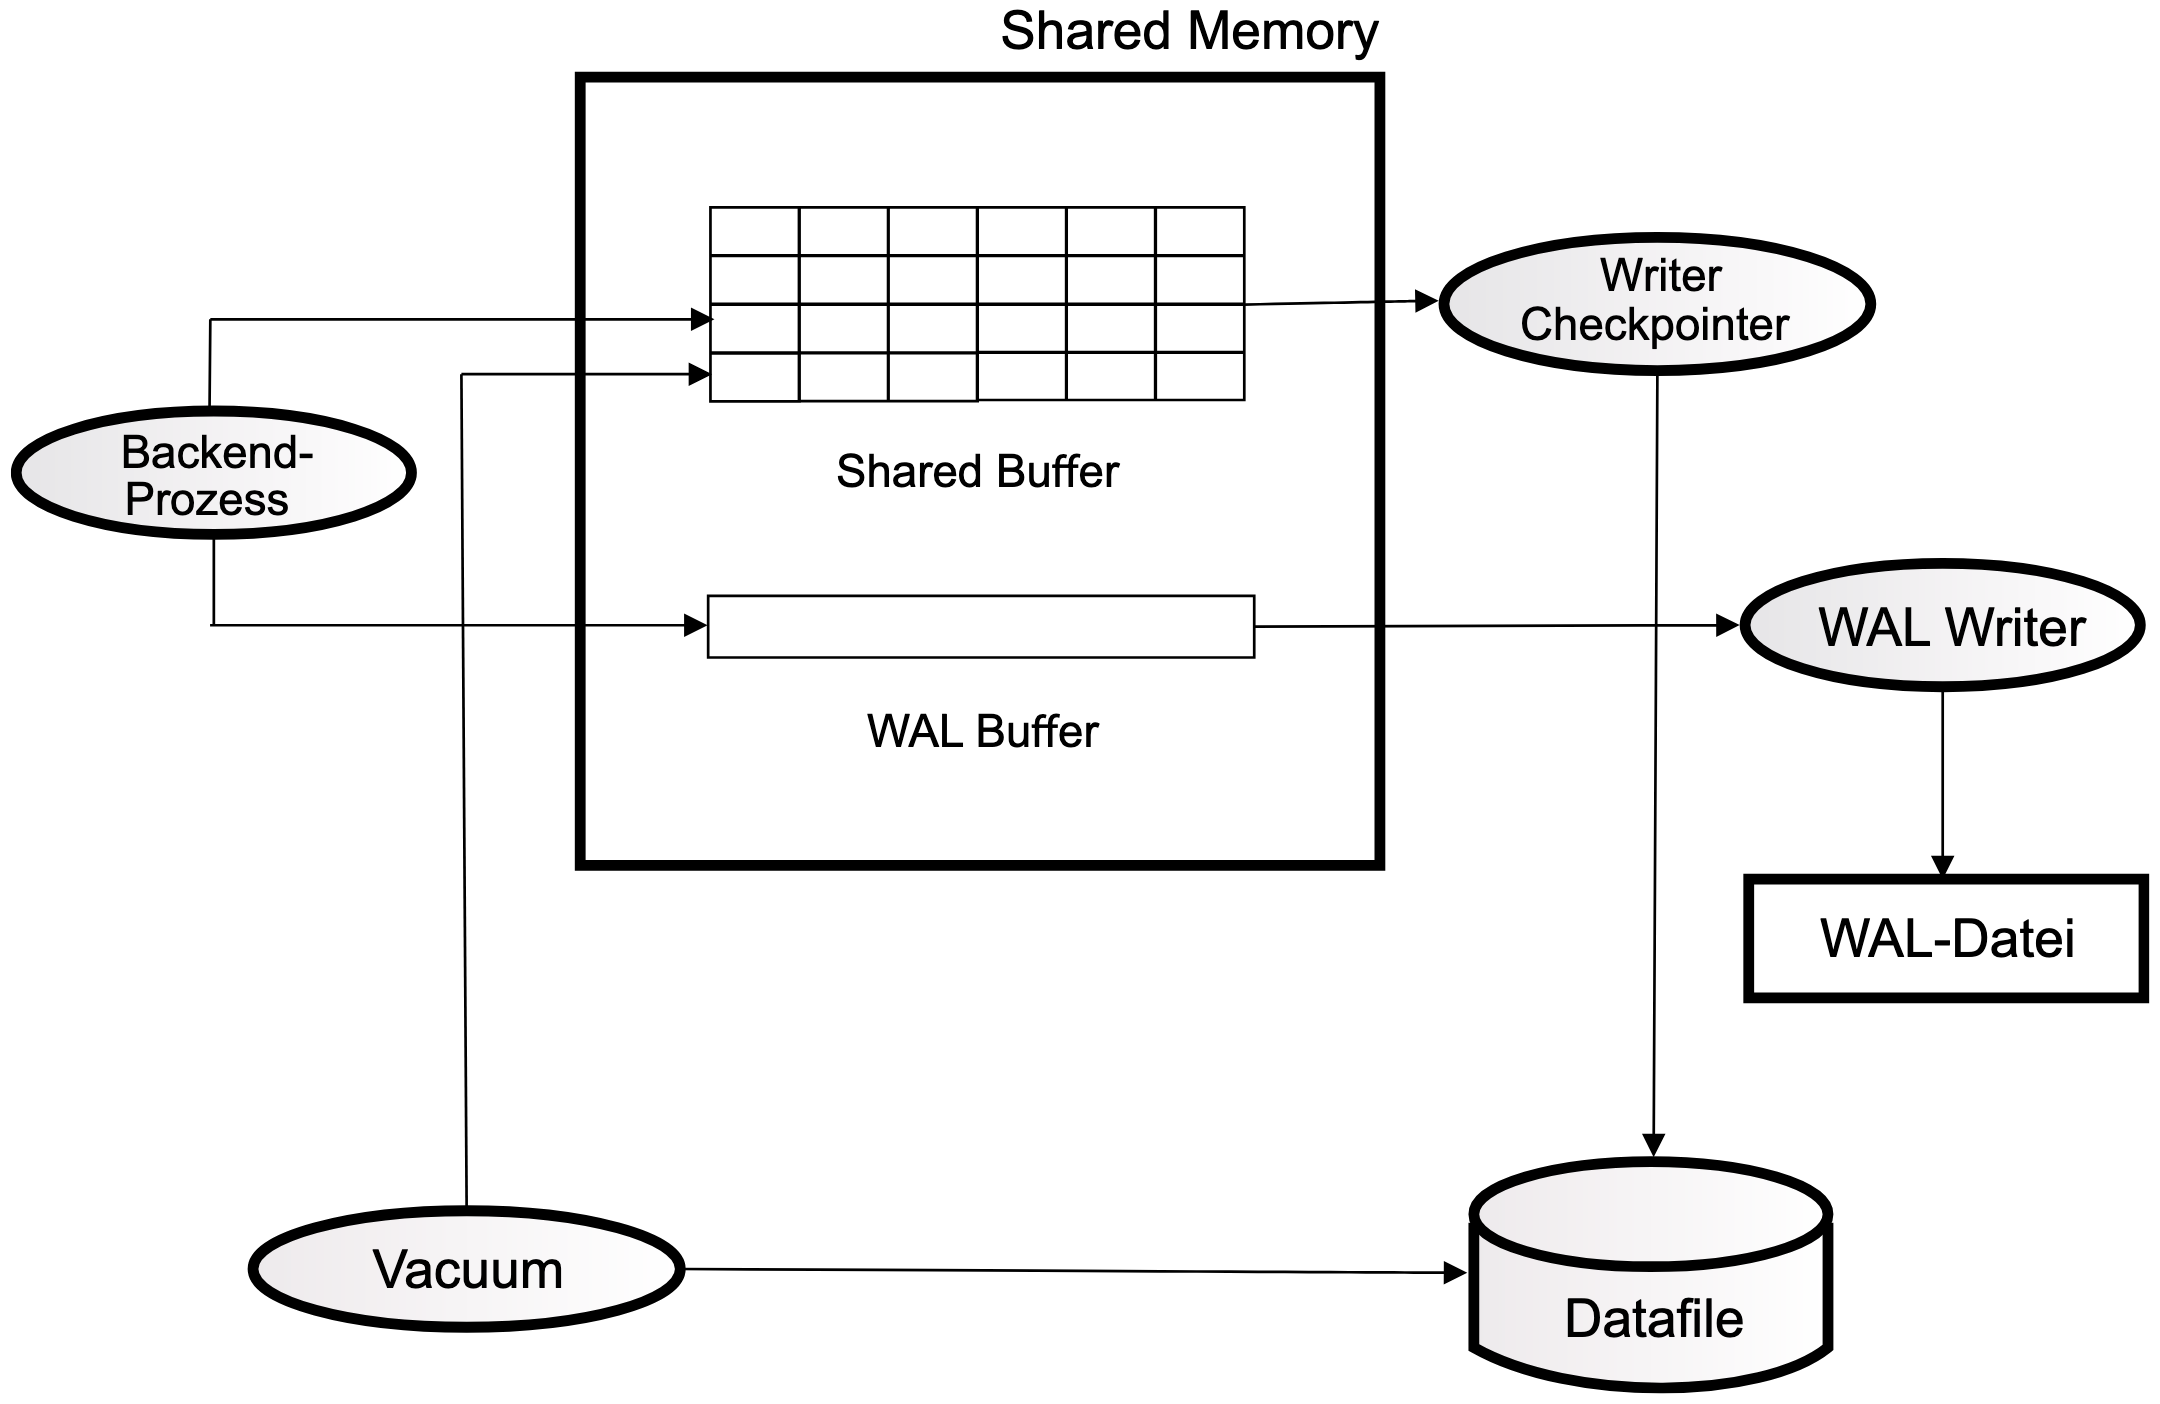
\includegraphics[width=\textwidth]{img/PostgreSQL Aufbau.png}
\caption{PostgreSQL Architektur. Quelle: \cite{Froehlich2022} S. 33 Bild 4.1}
\label{fig:Architektur}
\end{figure}

PostgreSQL besteht aus einer Kombination von Speicher und Prozessen. Bei Unix-Systemen sind diese Prozesse eigenständig, während sie bei Windows als Threads umgesetzt werden. Die wichtigsten Prozesse, die die Funktionalität von PostgreSQL abbilden, sind:
\begin{description}
    \item[Postmaster:] Der Hauptprozess, der die Verwaltung der anderen Prozesse übernimmt.
    \item[Checkpointer:] Dieser Prozess sorgt dafür, dass alle Änderungen in der Datenbank regelmäßig auf die Festplatte geschrieben werden.
    \item[Writer:] Verantwortlich für das Schreiben von geänderten Datenblöcken auf die Festplatte.
    \item[WAL Writer:] Handhabt das Schreiben von Transaktionsdaten in die Write-Ahead Log (WAL).
    \item[Autovacuum Launcher:] Dieser Prozess führt automatische Bereinigungen der Datenbank durch.
    \item[Archiver:] Archiviert die WAL-Dateien für eine verbesserte Rückverfolgbarkeit und Monitoring, besonders wichtig in produktiven Systemen.
    \item[Stats Collector:] Sammelt statistische Daten über die Nutzung von Sessions und Tabellen.
    \item[BGWorker:] Übernimmt verschiedene Hintergrundaufgaben.
\end{description}

\begin{figure}[h]
\centering
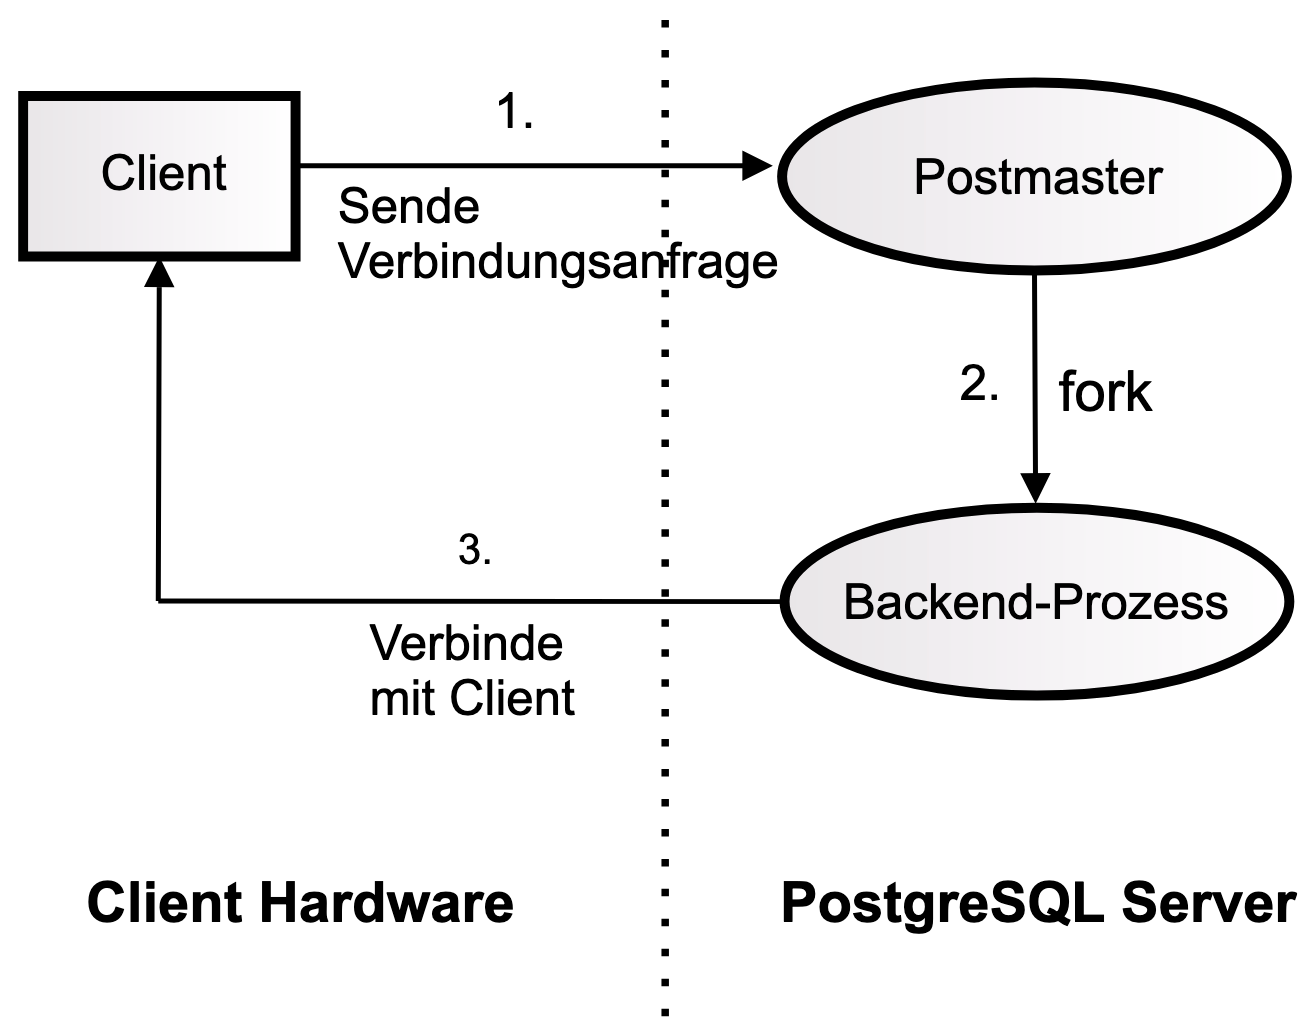
\includegraphics[width=\textwidth]{img/PostgreSQL Verbindungsaufbau.png}
\caption{Verbindungsaufbau von Client zum Server. Quelle: \cite{Froehlich2022} S. 35 Bild 4.3}
\label{fig:Verbindungsaufbau}
\end{figure}

Beim Aufbau einer Verbindung durch einen Client erstellt der Postmaster-Prozess nach erfolgreicher Authentifizierung und Autorisierung einen eigenen Backend-Thread. Die maximale Anzahl gleichzeitig aktiver Backend-Threads ist limitiert (Standard 100), was bedeutet, dass nach Erreichen dieser Grenze weitere Verbindungen abgelehnt werden.

\subsubsection{Speicherverwaltung und Performanceoptimierung}
Die Verwaltung von Speicher und die Optimierung der Zugriffszeiten auf Daten sind entscheidend für die Leistung von PostgreSQL. Da das Lesen von Daten von einer Festplatte vergleichsweise zeitaufwendig ist, setzt PostgreSQL auf verschiedene Mechanismen zur Verbesserung der Performance.

\begin{figure}[h]
\centering
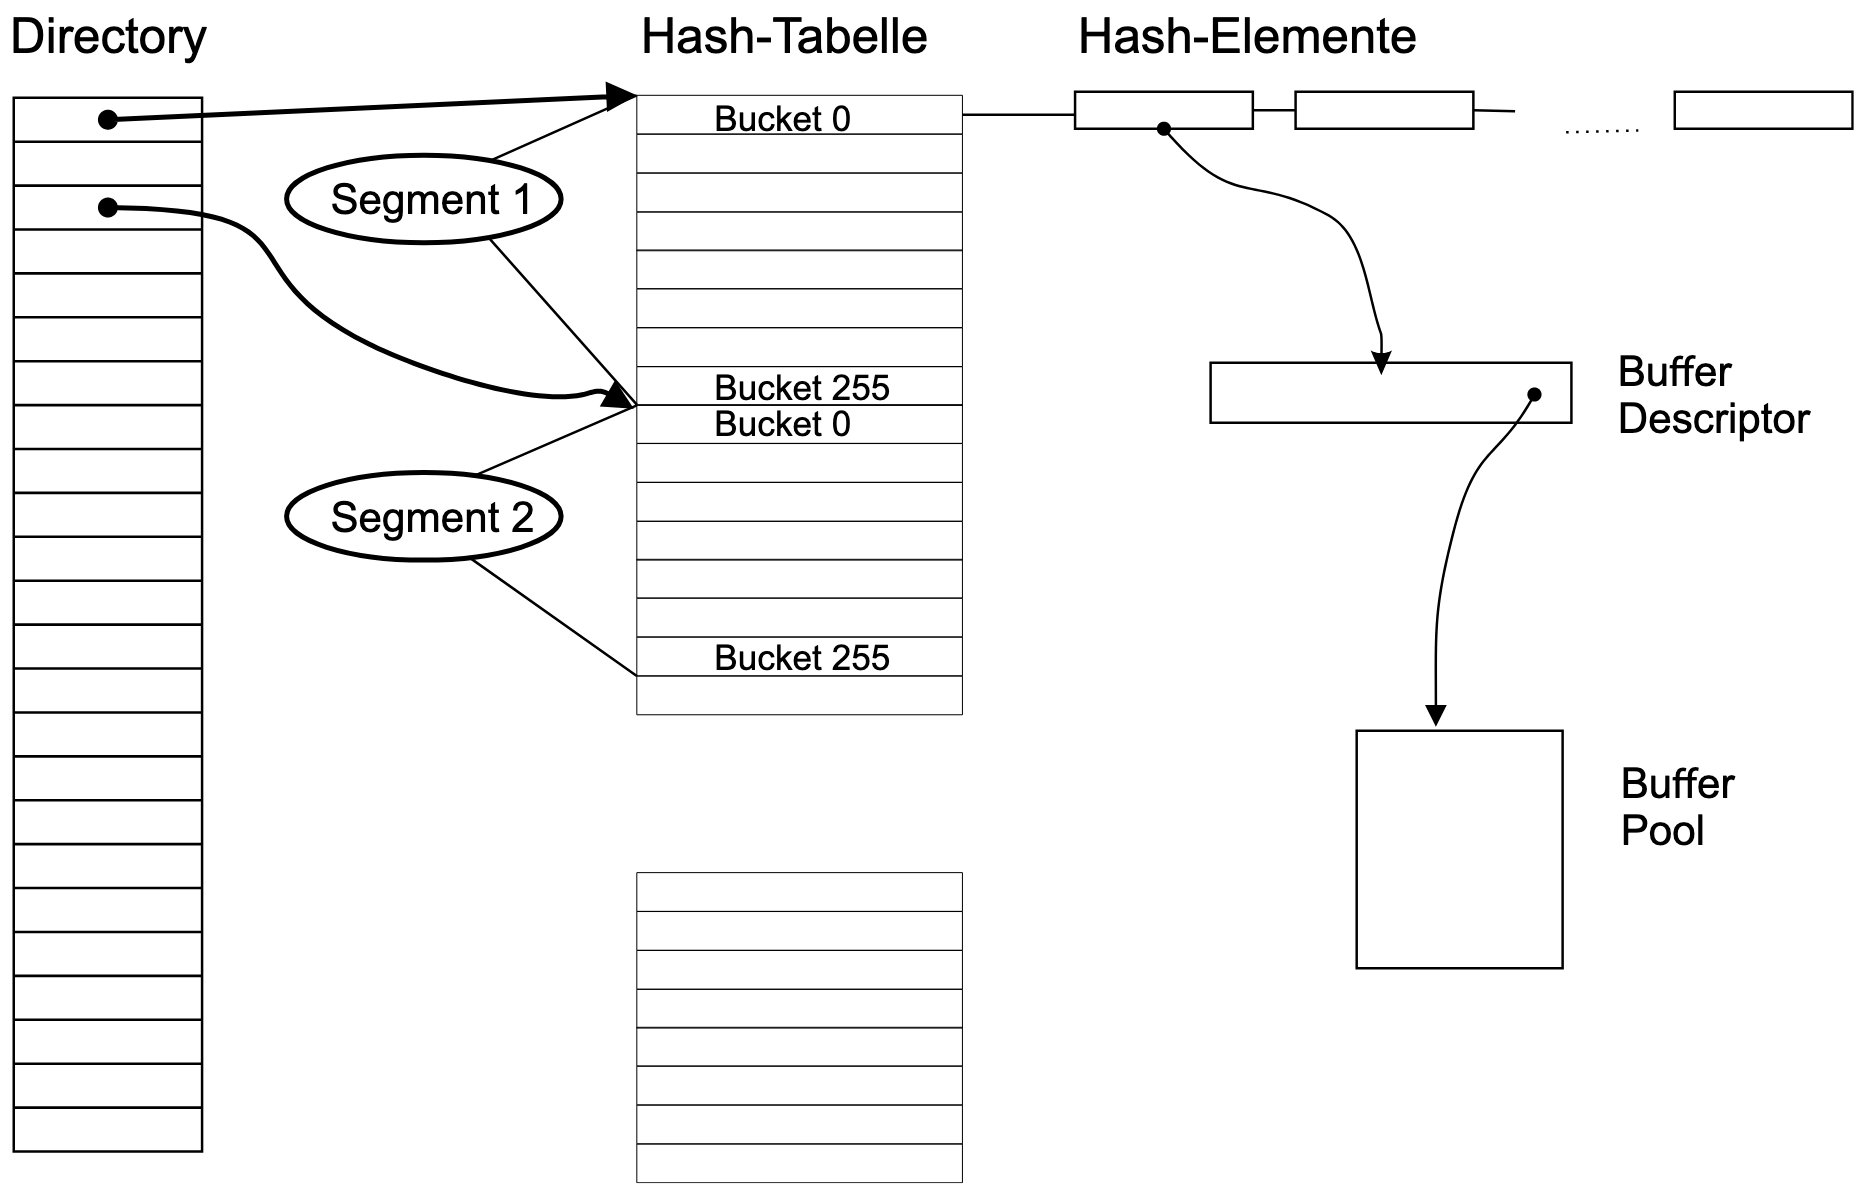
\includegraphics[width=\textwidth]{img/PostgreSQL Speciheraufbau.png}
\caption{PostgreSQL Speicherarchitektur. Quelle:  \cite{Froehlich2022} S. 37 Bild 4.4}
\label{fig:Speicheraufbau}
\end{figure}

\paragraph{Geteilter Speicher (Shared Buffer)}
Der Shared Buffer in PostgreSQL dient dazu, die Anzahl der Operationen auf der Festplatte zu reduzieren, indem er schnellen Speicher im RAM bereitstellt. Er besteht aus einer Hash-Tabelle, Hash-Elementen, einer Bufferbeschreibung und einer Buffersammlung. Die Hash-Tabelle ermöglicht ein schnelles Auffinden von Datensätzen, indem Hashwerte in Segmenten sortiert werden. Diese Segmente können sehr schnell durchsucht werden, da ihre Länge fest ist, was effiziente Speicherzugriffe ermöglicht.

Die Bufferbeschreibung enthält wichtige Steuerungsvariablen, wie z.B. den \code{\url{usage count}}, der die Relevanz eines Datensatzes im Speicher angibt. Der Speicherbereinigungsprozess (Eviction Process) durchsucht regelmäßig den Buffer nach irrelevanten Blöcken. Blöcke, die als irrelevant eingestuft werden, können überschrieben werden, sobald neuer Speicherplatz benötigt wird.

\paragraph{WAL Buffer und Checkpoints}
Der \ac{wal} Buffer ist darauf ausgelegt, Daten effizient auf die Festplatte zu schreiben. Dadurch müssen schreibende Prozesse nicht auf die tatsächliche Schreiboperation warten, sondern können die zu schreibenden Daten in den Buffer verlagern. Der \ac{wal} Buffer wird in regelmäßigen Intervallen (Standard 200 Millisekunden) überprüft und die Daten werden im Permanentspeicher gesichert, um die Ausfallsicherheit zu gewährleisten.

\code{Insert}-, \code{Update}- und \code{Delete}-Anweisungen werden über den \ac{wal}-Buffer verarbeitet. Diese Anweisungen werden in sogenannten \ac{wal}-Records gespeichert und sichern den Zustand der Daten auch bei einem Systemausfall. Ein Checkpoint, der den Speicherinhalt endgültig auf die Festplatte schreibt, wird unter bestimmten Bedingungen ausgeführt, wie etwa nach Ablauf eines festgelegten Intervalls, Erreichen einer bestimmten Buffergröße oder dem manuellen Auslösen eines Checkpoints.

\paragraph{Mehrere Datenblockversionen und Defragmentierung}

PostgreSQL unterstützt die gleichzeitige Bearbeitung von Datensätzen durch mehrere Sessions. Um sicherzustellen, dass sich die Sessions nicht gegenseitig beeinträchtigen, erhalten Datensätze eine Versionsnummer. Diese ermöglicht es, bei gleichzeitigen Abfragen und Bearbeitungen konsistente Daten bereitzustellen. Wenn eine Abfrage gestartet wird, kann anhand der Versionsnummer bestimmt werden, welcher Datensatz zum Zeitpunkt des Abfragestarts aktuell war.

Alte Datensätze, die nicht mehr benötigt werden, werden gelöscht, wodurch Lücken in der Tabelle entstehen. Diese Lücken werden durch den Autovacuum-Prozess freigegeben, sodass der Speicher für neue Datenblöcke verwendet werden kann. Bei Bedarf führt PostgreSQL ein \code{fullvacuum} durch, der die Tabelle vollständig defragmentiert, um Speicherplatz zurückzugewinnen und die Integrität der Versionsnummern zu gewährleisten.

\subsubsection{Permanentspeicherverwaltung}

Die Datenbanken von PostgreSQL werden im Verzeichnis \code{base} gespeichert, während der Tablespace in einem separaten Verzeichnis liegt. Tabellen und Indizes werden in Dateien von maximal einem Gigabyte Größe gespeichert; bei Überschreiten dieser Größe wird eine weitere Datei angelegt. Zusätzlich werden Dateien mit den Endungen \code{\_fsm} (Free Space Map) zur Adressierung des freien Speicherplatzes und \code{\_vm} (Visibility Map) zur Markierung von veralteten Datensätzen gepflegt.

Die Datenblocksammlung (Page) enthält Pointers auf die tatsächlichen Datenblöcke (Tuples). Jeder Datenblock wird durch eine Kombination aus der Datenblocksammlungsnummer und dem Offset des Pointers identifiziert. \cite{Froehlich2022}

\subsection{Exkurs: MongoDB}
MongoDB ist eine führende dokumentenorientierte NoSQL-Datenbank, die sich durch ihre Flexibilität und Skalierbarkeit auszeichnet. Sie wurde entwickelt, um einige der Einschränkungen traditioneller relationaler Datenbanken zu überwinden und bietet eine leistungsfähige Lösung für Anwendungen, die große Mengen an unstrukturierten oder semi-strukturierten Daten verarbeiten müssen. Im Gegensatz zu relationalen Datenbanken, die auf einem festen Schema basieren, erlaubt MongoDB ein dynamisches, schemaloses Datenmodell, das sich ideal für moderne, agile Entwicklungsprozesse eignet. In diesem Exkurs werden die Architektur und die technischen Merkmale von MongoDB detailliert beleuchtet, um deren Eignung für das \ac{nomtis}-Projekt zu bewerten.

\subsubsection{Speicherstruktur und Organisation}
MongoDB speichert Daten im \ac{bson}-Format, einem binären Format, das speziell für die Speicherung von Dokumenten mit \ac{json}-Syntax entwickelt wurde. \ac{bson} bietet eine effiziente Speicherung und Verarbeitung von Dokumenten, da es im Vergleich zu herkömmlichem \ac{json} kompakter und schneller zu verarbeiten ist. \ac{bson}-Dokumente können direkt in \ac{json} konvertiert werden, was die Integration mit Anwendungen erleichtert, die \ac{json} verwenden.

Die Speicherorganisation in MongoDB ist hierarchisch aufgebaut:
\begin{description}
    \item[Datenbank:] An der Spitze steht eine Datenbank, die mehrere Sammlungen (engl. Collections) enthalten kann.
    \item [Katalog:] Darunter befindet sich der Katalog, der Informationen über die Sammlungen und Indizes speichert.
    \item [Sammlung (engl. Collection)]: Eine Sammlung ist eine Gruppe von Dokumenten, die thematisch zusammengehören und ähnliche Strukturmerkmale aufweisen.
    \item [Dokument:] Auf der untersten Ebene steht das Dokument, das die eigentlichen Daten enthält.
\end{description}

\subsubsection{Katalog und Speicherverwaltung}

Der Katalog von MongoDB ist für die Verwaltung der Metadaten von Sammlungen und Indizes verantwortlich. Es gibt zwei Arten von Katalogen:
\begin{description}
    \item[Persistenter Katalog:] Dieser speichert Informationen dauerhaft auf der Festplatte und stellt sicher, dass Metadaten auch nach einem Neustart des Systems verfügbar bleiben. Der persistente Katalog wird in BSON-Dateien mit der Endung \code{\_mdb\_catalog} gespeichert und enthält Details über die Eigenschaften und Indizes der Sammlungen.
    \item [Memory-Katalog:] Der Memory-Katalog hält die Metadaten im RAM vor, um schnellen Zugriff zu gewährleisten und Ladezeiten zu minimieren. Operationen wie das Erstellen, Suchen, Iterieren und Schließen von Sammlungen werden im Memory-Katalog durchgeführt.
\end{description}

Um Dateninkonsistenzen zu vermeiden, wird der Memory-Katalog regelmäßig mit dem persistenten Katalog synchronisiert. Eine Versionsverwaltung stellt sicher, dass Änderungen korrekt nachvollzogen werden können, ohne dass es zu Lese-Schreib-Kollisionen kommt. MongoDB verwendet dabei das Copy-on-Write-Prinzip, bei dem nur dann eine Kopie des Datensatzes erstellt wird, wenn tatsächlich Änderungen vorgenommen werden. Dies minimiert den Speicherbedarf und erhöht die Effizienz.

\subsubsection{Speicherverwaltung und Defragmentierung}
Beim Löschen eines Eintrags in MongoDB erfolgt dieser Prozess in zwei Schritten:
\begin{enumerate}
    \item Löschen des Katalogeintrags: Zunächst wird der Eintrag sowohl im Memory-Katalog als auch im persistenten Katalog entfernt. Ein Verweis auf die Sammlung wird an den sogenannten \glqq Reaper\grqq{} übergeben, um sicherzustellen, dass keine neuen Zugriffe auf die Sammlung erfolgen, während aktive Lesezugriffe abgeschlossen werden.
    \item Endgültiges Löschen: Nachdem sichergestellt wurde, dass kein Rollback erfolgen kann, der die Daten der Sammlung wiederherstellen könnte, werden die Daten endgültig gelöscht.
\end{enumerate}

Freier Speicher, der durch das Löschen von Daten entsteht, wird in regelmäßigen Abständen für neue Datensätze freigegeben. Wenn der Speicher fragmentiert wird und viele kleine Lücken entstehen, führt MongoDB eine Defragmentierung durch. Dieser Prozess ordnet den Speicher neu an, kann jedoch Lese- und Schreiboperationen blockieren, was die Performance beeinträchtigen könnte. Daher sollte die Defragmentierung möglichst selten durchgeführt werden.

\subsubsection{Indizes und Abfragen}
Indizes in MongoDB werden hauptsächlich als B-Baum-Strukturen gespeichert, die eine effiziente Suche und Sortierung von Daten ermöglichen. Ein B-Baum-Index speichert die Daten strukturiert, ähnlich wie ein Dokument, und ermöglicht schnelle Zugriffe auf häufig abgefragte Felder. MongoDB erlaubt es auch, benutzerdefinierte Speicherstrukturen für Indizes zu erstellen, um spezifische Anwendungsanforderungen zu erfüllen. \cite{IamXander2024} \cite{themattman2024}

\subsubsection{BSON - Binary JSON}

\ac{bson} ist das zugrunde liegende Format für die Speicherung von Dokumenten in MongoDB. Es handelt sich dabei um ein binäres Format, das sogenannte Key-Value-Paare speichert und direkt in \ac{json} konvertiert werden kann. \ac{bson} ist jedoch deterministischer als \ac{json}, da es keine Flexibilität in der Darstellungsform bietet. Dies bedeutet, dass ein Datensatz in \ac{bson} immer in einer einzigen, festen Form dargestellt wird.

Ein \ac{bson}-Dokument beginnt immer mit einem 32-Bit-Ganzzahlwert, der die Länge des Dokuments angibt, und endet mit einem Null-Byte. Aufgrund dieser Struktur kann ein \ac{bson}-Dokument maximal ca. 2,147 Gigabyte an Daten umfassen. Die verschiedenen Datentypen, die \ac{bson} unterstützt, umfassen unter anderem:
\begin{description}
    \item[Int32 und Int64:] 4- bzw. 8-Byte lange Ganzzahlen.
    \item[Double:] 8-Byte lange Gleitkommazahlen nach dem IEEE 754-Standard.
    \item[Decimal128:] 16-Byte lange Gleitkommazahlen für hohe Präzision.
    \item[Array:] Ein Feld, das eine Liste von Werten speichert, wobei die Elemente wie Dokumente behandelt werden.
    \item[Null-Wert:] Ein spezieller Marker, der das Fehlen eines Wertes kennzeichnet.
    \item[Min- und Max-Schlüssel:] Marker, die den minimalen bzw. maximalen Wert eines Feldes darstellen.
\end{description}

Die strikte Struktur von \ac{bson} sorgt für eine konsistente und effiziente Speicherung und Verarbeitung von Dokumenten, was MongoDB zu einer leistungsfähigen Lösung für Anwendungen macht, die flexible und skalierbare Datenbanken benötigen. \cite{Velikhov}

\subsection{Diskurs: Vergleich von PostgreSQL und MongoDB für NOMTIS}
Die Auswahl der geeigneten Datenbanklösung ist ein zentraler Aspekt bei der Entwicklung von \ac{nomtis}. Da die internen Richtlinien PostgreSQL und MongoDB als verfügbare Optionen vorsehen, ist es entscheidend, die spezifischen Anforderungen von \ac{nomtis} zu analysieren und zu bestimmen, welche der beiden Datenbanken diese am besten erfüllt.

\subsubsection{Technische Anforderungen an NOMTIS}
\ac{nomtis} muss Benachrichtigungen effizient speichern, verwalten und flexibel verarbeiten können. Ein Hauptmerkmal von \ac{nomtis} ist die Fähigkeit, Benachrichtigungen mit potenziell komplexen und verschachtelten Datenstrukturen zu verwalten. Diese Datenstrukturen können variieren und sind oft nicht im Voraus vollständig definiert. Zudem sind eine hohe Zuverlässigkeit, Konsistenz und Skalierbarkeit erforderlich, um den Anforderungen eines modernen Benachrichtigungssystems gerecht zu werden.

\subsubsection{PostgreSQL: Technische Stärken und Grenzen}
PostgreSQL ist eine relationale Datenbank, die für ihre starke Unterstützung von \ac{acid}-Transaktionen, Datenintegrität und komplexen relationalen Abfragen bekannt ist. Diese Eigenschaften machen PostgreSQL ideal für Anwendungen, bei denen strenge Konsistenzanforderungen und komplexe Datenbeziehungen im Vordergrund stehen.

Die feste Struktur von PostgreSQL kann jedoch zu Einschränkungen führen, wenn es darum geht, dynamische und verschachtelte Datenstrukturen zu verwalten. Änderungen am Datenmodell erfordern eine Anpassung des Schemas, was in einem dynamischen Umfeld, wie es \ac{nomtis} erfordert, potenziell problematisch sein kann. Zudem ist PostgreSQL weniger effizient im Umgang mit tief verschachtelten oder unvorhersehbaren Datenstrukturen, was die Flexibilität des Systems einschränken könnte.

\subsubsection{MongoDB: Flexibilität und Skalierbarkeit}
MongoDB hingegen ist eine dokumentenorientierte NoSQL-Datenbank, die sich durch ihre schemalose Architektur und hohe Flexibilität auszeichnet. Die Speicherung erfolgt im BSON-Format, das eine effiziente Handhabung von \ac{json}-ähnlichen Dokumenten ermöglicht. Diese Struktur erlaubt es, Daten ohne festes Schema zu speichern, was für \ac{nomtis} von Vorteil ist, da die Benachrichtigungen beliebig komplexe und verschachtelte Daten enthalten können.

Ein weiterer zentraler Vorteil von MongoDB ist seine horizontale Skalierbarkeit. MongoDB unterstützt das sogenannte \glqq Sharding \grqq, bei dem Daten über mehrere Server verteilt werden, um eine hohe Verfügbarkeit und Performance sicherzustellen. Diese Fähigkeit zur horizontalen Skalierung ist besonders in einer Umgebung wie der \ac{sit} von Bedeutung, wo das Datenvolumen und die Anzahl der Nutzer kontinuierlich wachsen können.

Laut einer Untersuchung der MongoDB-Datenbank von Anjali Chauhan bietet MongoDB darüber hinaus eine hohe Leistung durch die Verwendung eingebetteter Datenmodelle, die E/A-Aktivitäten reduzieren, sowie durch Indizes, die schnellere Abfragen ermöglichen. \cite{Chauhan2019}
Diese Leistungsmerkmale machen MongoDB besonders geeignet für Anwendungen, die auf hohe Geschwindigkeit und effizienten Datenzugriff angewiesen sind.

\subsubsection{Schlussfolgerung: PostgreSQL als geeignete Wahl für Sensora}
Im Projekt Sensora ergibt sich aus den strukturellen Anforderungen und den funktionalen Zugriffsmustern ein klarer Bedarf an einem relationalen, transaktional konsistenten Datenbanksystem. Die Datenstruktur ist vordefiniert und weitgehend stabil. Pflanzen, Sensoren, Aktoren, Gruppen und Räume bilden klar abgegrenzte Entitäten mit definierten Beziehungen zueinander. Diese Relationen sind nicht nur logisch konzipiert, sondern stellen funktionale Notwendigkeiten dar – etwa wenn Sensoren bestimmten Pflanzen zugeordnet sind oder Aktionen nur innerhalb definierter Gruppenzugehörigkeiten zulässig sind.

Die Abfrageanforderungen im operativen Betrieb bestehen aus einer Mischung aus punktuellen Zugriffen (etwa auf aktuelle Sensorwerte oder Soll-Ist-Vergleiche) und zeitbasierten Auswertungen über große Datenmengen – insbesondere für die letzten 24 Stunden. Diese Anforderungen sind auf ein konsistentes, indexoptimiertes Schema angewiesen, das Joins effizient unterstützt und sich nicht durch Schema-Flexibilität, sondern durch strukturelle Integrität auszeichnet. Gleichzeitig ist paralleler Zugriff durch mehrere Microservices erforderlich, sodass Transaktionssicherheit und Isolation nicht nur erwünscht, sondern notwendig sind, um Inkonsistenzen bei konkurrierenden Schreiboperationen zu vermeiden.

PostgreSQL bietet genau für diese Art von Workload die passende Grundlage. Die stark normierten Strukturen des Sensora-Datenmodells profitieren von PostgreSQLs ausgefeilter Optimierung relationaler Abfragen, der zuverlässigen Durchsetzung referenzieller Integrität sowie der Möglichkeit, durch gezieltes Indexing auf Zeitstempel-Feldern hochfrequente historische Abfragen performant abzubilden. Selbst bei wachsendem Datenvolumen lassen sich durch Partitionierung oder die spätere Ergänzung durch TimescaleDB – ohne Verlassen der PostgreSQL-Basis – die Performanceanforderungen langfristig erfüllen, ohne strukturelle Kompromisse einzugehen.

Die fehlende Notwendigkeit für dynamische Schemas, polymorphe Dokumente oder eingebettete Strukturen eliminiert die Hauptargumente für ein dokumentenbasiertes System wie MongoDB. Vielmehr würde dessen Flexibilität in diesem Kontext eher potenzielle Inkonsistenzen begünstigen und zusätzliche Validierungslogik auf Anwendungsebene erforderlich machen – ein Mehraufwand, der durch das klar strukturierte Datenmodell nicht gerechtfertigt ist.

In Summe ist PostgreSQL damit nicht nur die technisch bessere Wahl, sondern die natürlichere Fortsetzung der bereits im Projektdesign angelegten Prinzipien: strukturierte, konsistente und integrierte Datenhaltung, auf die performant und sicher gleichzeitig von vielen Systemkomponenten zugegriffen werden kann.

        \section{Auswahl der Technologien f\"ur die entwickelten \\ Schnittstellen-Services}

Die im Rahmen des Projekts \textit{Sensora} entwickelten Schnittstellen-Services \"ubernehmen unterschiedliche Aufgaben innerhalb der Systemarchitektur, stellen jedoch alle zentrale Bausteine zur Kommunikations- und Steuerungsebene dar. Ihre Implementierung erfordert eine wohl\"uberlegte Auswahl geeigneter Technologien, die sowohl den funktionalen Anforderungen als auch den architekturellen, sicherheitstechnischen und betrieblichen Rahmenbedingungen gerecht werden.

In diesem Kapitel werden die getroffenen Technologieentscheidungen f\"ur jeden entwickelten Service einzeln erl\"autert, mit vergleichbaren Alternativen kontextualisiert und unter R\"uckbezug auf die definierten Anforderungen begr\"undet.

\subsection{Technologieauswahl f\"ur den Authentifizierungs- und Registrierungsdienst (Auth-Service)}

\subsubsection*{Zielsetzung und Kontext}

Der Auth-Service ist eine der sicherheitskritischsten Komponenten des Sensora-Systems. Er ist daf\"ur verantwortlich, neue IoT-Controller kontrolliert ins System aufzunehmen, ihnen eindeutige Kommunikationsidentit\"aten zuzuweisen und die Authentizit\"at dieser Ger\"ate eindeutig zu \"uberpr\"ufen. Zudem verwaltet er die Registrierung von Controllern in der zentralen Datenbank und erzeugt differenzierte Zugriffskan\"ale innerhalb der Messaging-Infrastruktur.

\subsubsection*{Verwendete Programmiersprache: Python}

F\"ur die Umsetzung des Auth-Service wurde die Programmiersprache \textbf{Python} gew\"ahlt. Python bietet eine sehr hohe Ausdrucksst\"arke bei gleichzeitig niedriger Komplexit\"at in der Syntax\cite{python_flask_prototyping}. Dies erlaubt eine fokussierte Umsetzung sicherheitskritischer Logik mit hoher Lesbarkeit und reduziertem Fehlerpotenzial. Die Sprache bietet native Unterst\"utzung f\"ur REST-APIs (via Flask), HMAC-Berechnungen (via \texttt{hashlib}) und JSON-Verarbeitung, was sie ideal f\"ur die Umsetzung des Auth-Service macht.

Im Vergleich zu Alternativen wie Java oder Go zeigt Python zwar leistungstechnische Schw\"achen bei hochfrequenten Systemen, bietet daf\"ur jedoch wesentlich h\"ohere Entwicklungsproduktiv\"itat \textendash{} ein entscheidender Vorteil im Rahmen eines begrenzten studentischen Projektzeitraums.

\paragraph*{Alternative Bewertung:}

Java bietet mit Spring Security zwar eine \"au\ss{}erst robuste Infrastruktur f\"ur Authentifizierungsmechanismen, ist jedoch deutlich komplexer im Deployment und ben\"otigt mehr Konfigurationsaufwand. Go bietet starke Performance und native Concurrency-Modelle, jedoch eine im Vergleich zu Python eingeschr\"ankte Bibliothekslandschaft f\"ur Security-Workflows. 

\paragraph*{Begr\"undung der Auswahl:}

Angesichts der Priorisierung von Entwicklungszeit, Lesbarkeit, Testbarkeit und Verf\"ugbarkeit passender Security-Tools wurde Python als die geeignetste Sprache f\"ur den Auth-Service identifiziert.

\subsubsection*{Authentifizierungsmechanismus: HMAC-basiertes Challenge-Response-Verfahren}

F\"ur die Authentifizierung der IoT-Ger\"ate wurde ein leichtgewichtiges Challenge-Response-Verfahren auf Basis von HMAC (Hash-based Message Authentication Code) implementiert. Diese Entscheidung basiert auf den Anforderungen an ein sicheres, serverseitig validierbares Verfahren ohne Notwendigkeit, Klartext-Zugangsdaten zu speichern oder zu \"ubertragen.

\paragraph*{Alternative Technologien:}
\begin{itemize}
  \item \textbf{OAuth 2.0:} Standard f\"ur Benutzer-Authentifizierung, jedoch komplex in der Implementierung f\"ur Maschinen-zu-Maschinen-Kommunikation.
  \item \textbf{JWT (JSON Web Token):} Geeignet f\"ur Token-basierte Sessions, jedoch problematisch hinsichtlich Zustandslosigkeit bei Ger\"aten mit hohem Sicherheitsanspruch.
  \item \textbf{Client-Zertifikate:} Sehr sicher, aber schwergewichtig in der Verwaltung f\"ur dynamisch zu registrierende IoT-Ger\"ate.
\end{itemize}

\paragraph*{Begr\"undung der Auswahl:}

Das HMAC-Verfahren erm\"oglicht die Validierung eines vorab generierten Ger\"ateschl\"ussels (Token), ohne diesen selbst senden zu m\"ussen. Durch serverseitige Generierung einer Challenge, die vom Ger\"at korrekt beantwortet werden muss, wird ein sicheres, manipulationsresistentes Protokoll etabliert, das gleichzeitig ressourcenschonend und einfach zu implementieren ist. Die Entscheidung orientiert sich damit an Best Practices f\"ur Ger\"ateauthentifizierung in Embedded-Umgebungen \cite{rfc2104_hmac}.

\subsubsection*{Kommunikationsmodell: REST-basierte API}

Der Service stellt seine Funktionalit\"at \"uber HTTP/REST-Endpunkte zur Verf\"ugung. Die Entscheidung f\"ur ein REST-Modell basiert auf der Notwendigkeit, den Dienst sowohl von Web-Frontends als auch von anderen Services (z.\,B. Mail-Service oder Solace-Konfiguration) ansprechbar zu machen.

\paragraph*{Alternative Technologien:}
\begin{itemize}
  \item \textbf{gRPC:} Hohe Effizienz, jedoch schwerer in Browser-Umgebungen integrierbar.
  \item \textbf{MQTT:} Bietet nur Publish/Subscribe, nicht geeignet f\"ur Request/Response-Workflows mit stateless APIs.
\end{itemize}

\paragraph*{Begr\"undung:}

REST bietet mit seiner stateless Architektur und breiten Toolunterst\"utzung (z.\,B. Swagger, Postman, curl) die optimale Basis f\"ur verteilte Systeme, insbesondere f\"ur administrative Operationen wie die Controller-Registrierung.

\subsubsection*{Interner Konfigurationsspeicher: JSON-Datei}

Die Informationen \"uber aktive Challenges und bereits registrierte Ger\"ate werden zus\"atzlich zur Datenbank in einer strukturierten JSON-Datei gespeichert. Dies erm\"oglicht schnelle Zugriffe auf tempor\"are Daten ohne Overhead einer persistierten Transaktion. Dieser pragmatische Kompromiss ist im Kontext studentischer Prototypen vertretbar.

\subsection{Technologieauswahl f\"ur den E-Mail-Verifikationsdienst (Mail-Service)}

\subsubsection*{Zielsetzung und Kontext}

Der Mail-Service stellt eine sicherheitsrelevante Verbindung zwischen Benutzerschnittstellen und Backend dar. Seine prim\"are Aufgabe ist die Versendung von E-Mail-\\Verifizierungslinks nach der Benutzerregistrierung. Damit fungiert er als zentrale Instanz zur initialen Verifikation von Benutzeridentit\"aten. Neben der Kommunikation mit einem SMTP-Server stellt der Dienst auch eine kontrollierte API zur Entgegennahme von Verifizierungsanfragen bereit.

\subsubsection*{Verwendete Programmiersprache: Python}

Die Entscheidung f\"ur Python basiert auf \"ahnlichen Argumenten wie beim Auth-Service. Python bietet durch Bibliotheken wie \texttt{smtplib} und \texttt{email.mime} einfache Schnittstellen zur Realisierung von SMTP-Kommunikation. Zus\"atzlich erlaubt die Verwendung von Flask eine unkomplizierte REST-Anbindung mit geringen Komplexit\"atsh\"urden. Im Rahmen des Projekts erm\"oglichte dies eine schnelle, wartbare und lesbare Implementierung des Dienstes.

\paragraph*{Vergleich mit Alternativen:}

Java (z.\,B. mit Spring Boot Mail) h\"atte eine robustere Infrastruktur geboten, w\"are jedoch mit erheblich h\"oherem Konfigurationsaufwand verbunden gewesen. Node.js wiederum bietet durch Pakete wie \texttt{nodemailer} eine gute Grundlage, ist jedoch im Team hinsichtlich Erfahrung weniger etabliert gewesen.

\paragraph*{Begr\"undung der Auswahl:}

Im Hinblick auf Entwicklungszeit, Lesbarkeit, Bibliotheksunterst\"utzung und Teamkompetenz wurde Python als pragmatische und effektive L\"osung gew\"ahlt.

\subsubsection*{E-Mail-Kommunikationsprotokoll: SMTP \"uber TLS}

F\"ur den Versand von Verifizierungsnachrichten wurde das Simple Mail Transfer Protocol (SMTP) in Kombination mit einer Transport Layer Security (TLS)-Verbindung eingesetzt. Diese Kombination bietet einen etablierten Standard f\"ur ausgehende Mail-Kommunikation mit Basisverschl\"usselung.\cite{smtp_tls}

\paragraph*{Alternativen:}

\begin{itemize}
  \item \textbf{REST-basierte Mailservices (z.\,B. SendGrid, Mailgun):} Bieten einfache APIs und statistische Auswertung, erfordern aber Drittanbieterkonten und externe Infrastruktur.
  \item \textbf{SMTP ohne Verschl\"usselung:} Unsicher und nicht datenschutzkonform.
\end{itemize}

\paragraph*{Begr\"undung:}

Die Entscheidung f\"ur SMTP \"uber TLS wurde getroffen, da ein Gmail für eine nicht zu Hohe Menge an Mails dies kostenlos ermöglicht und bereits zur Verf\"ugung stand und keine Drittanbieterintegration gew\"unscht war. Gleichzeitig konnten Sicherheitsanforderungen gewahrt bleiben.

\subsubsection*{Zugriffsschutz: Pre-Shared Key (PSK)}

Um zu verhindern, dass Dritte beliebige Verifizierungsanfragen senden, wurde der REST-Endpunkt des Mail-Service mit einem Pre-Shared Key abgesichert. Nur Systeme, die diesen kennen, k\"onnen autorisiert E-Mails ausl\"osen.

\paragraph*{Alternative Schutzmechanismen:}
\begin{itemize}
  \item \textbf{OAuth 2.0 oder API Tokens:} Sicher, aber unn\"otig komplex f\"ur einen geschlossenen Service.
  \item \textbf{Keine Authentifizierung:} Sicherheitsrisiko.
\end{itemize}

\paragraph*{Begr\"undung:}

Der Einsatz eines PSK ist ein einfacher, aber effektiver Schutzmechanismus, der in einem geschlossenen Systemumfeld wie Sensora praktikabel und ausreichend sicher ist.

\subsection{Technologieauswahl f\"ur den Datenpersistenzdienst (Database Writer)}

\subsubsection*{Zielsetzung und Kontext}

Der Database Writer nimmt eine zentrale Rolle in der persistenznahen Verarbeitung eingehender Sensordaten ein. Seine Hauptaufgabe besteht darin, kontinuierlich Datenpakete aus der Messaging-Infrastruktur entgegenzunehmen, diese auszuwerten und in strukturierter Form in das zugrunde liegende Datenbanksystem zu \"ubertragen. Eine besondere Herausforderung besteht dabei in der Notwendigkeit, sowohl hohe Verf\"ugbarkeit als auch Integrit\"at der Messdaten zu gew\"ahrleisten, selbst bei tempor\"aren Netzwerkproblemen oder inkonsistenten Eingangsnachrichten.

\subsubsection*{Programmiersprache: Python}

Die Implementierung des Database Writers erfolgte in Python. Die Entscheidung basiert auf der Kombination aus vorhandener Expertise im Projektteam, umfangreicher Bibliotheksunterstützung für JSON-Verarbeitung, Messaging-Systeme und Datenbankzugriffe sowie der leichten Wartbarkeit der Servicestruktur. In Python stehen mit Bibliotheken wie \texttt{paho-mqtt}\cite{python_mqtt}, \texttt{psycopg2} und \texttt{json} sofort einsatzfähige und stabile Werkzeuge für alle Teilaufgaben zur Verfügung.

\paragraph*{Vergleich mit Alternativen:}

Eine Implementierung in Go w\"are performant und speichereffizient, jedoch mit deutlich h\"oherem Aufwand bei der Bibliotheksintegration verbunden gewesen. Java h\"atte ebenfalls umfassende JDBC-basierte Anbindungen an relationale Datenbanken geboten, ist aber insbesondere f\"ur prototypische Implementierungen \"uberdimensioniert und aufw\"andig in Bezug auf Konfiguration und Deployment.

\paragraph*{Begr\"undung:}

Die Wahl von Python stellt einen optimalen Kompromiss zwischen Funktionalit\"at, Einfachheit und Flexibilit\"at dar. Dar\"uber hinaus konnte die gemeinsame Sprache mit den \"ubrigen Schnittstellen-Services genutzt werden, was die Homogenit\"at und Wartbarkeit der Gesamtplattform verbessert.

\subsubsection*{Messaging-Empfang: MQTT}

Der Database Writer konsumiert eingehende Nachrichten \"uber das MQTT-Protokoll, das vom zentralen Messaging-System vermittelt wird. MQTT wurde ausgew\"ahlt, da es mit seinem Publish/Subscribe-Paradigma und dem minimalen Protokoll-Overhead ideal auf intermittierende und latenzempfindliche Kommunikationsbeziehungen zwischen Sensoren und Auswertungssystemen zugeschnitten ist.\cite{mqtt_overview}

\paragraph*{Alternative Protokolle:}

\begin{itemize}
  \item \textbf{AMQP:} Industriestandard f\"ur Messaging, jedoch schwergewichtiger und nicht speziell f\"ur IoT optimiert.
  \item \textbf{HTTP Push:} Einfach zu implementieren, aber ungeeignet f\"ur kontinuierliche, bidirektionale Datenstr\"ome.
  \item \textbf{WebSockets:} Echtzeitf\"ahig, jedoch komplexer in der Integration mit klassischen Persistenzsystemen.
\end{itemize}

\paragraph*{Begr\"undung:}

MQTT bietet ein exzellentes Gleichgewicht zwischen Zuverl\"assigkeit, Ressourceneffizienz und Verbreitung im IoT-Bereich. Die Persistenzfunktionen des zugrunde liegenden Messaging-Brokers stellen zudem sicher, dass keine Daten durch kurzzeitige Netzwerkausf\"alle verloren gehen.

\subsubsection*{Fehlerbehandlung und Wiederholungsmechanismen}

Im Database Writer wurden explizite Retry-Mechanismen f\"ur die Datenbankanbindung integriert, um Datenverluste bei vor\"ubergehender Nichtverf\"ugbarkeit zu verhindern. Dies erfolgt \"uber ein warteschlangenbasiertes Zwischenspeichern nicht erfolgreicher Schreiboperationen, die periodisch erneut angesto\"ossen werden.

\paragraph*{Alternative Ans\"atze:}

\begin{itemize}
  \item \textbf{Fire-and-Forget-Ansatz:} Einfach, aber inakzeptabel bei Sicherheits- oder Zuverl\"assigkeitsanforderungen.
  \item \textbf{Transaktionsbasierte Protokolle:} W\"aren robuster, jedoch mit hohem Implementierungsaufwand verbunden.
\end{itemize}

\paragraph*{Begr\"undung:}

Die gew\"ahlte Methode stellt sicher, dass Datenverlust unter realistischen Bedingungen nahezu ausgeschlossen ist, ohne den Entwicklungsaufwand \"uber Geb\"uhr zu erh\"ohen. Die Wiederholungslogik kann bei Bedarf skalierbar erweitert werden.

\subsection{Technologieauswahl f\"ur die Zielwert-Schnittstelle (Setpoint API)}

\subsubsection*{Zielsetzung und Kontext}

Die Setpoint API erm\"oglicht die gezielte \"Ubertragung von Sollwerten an Steuercontroller, welche wiederum f\"ur die Regelung der Wasserzufuhr einzelner Pflanzen verantwortlich sind. Damit bildet sie eine Br\"ucke zwischen Benutzeranwendungen bzw. Systemkomponenten mit Steuerlogik und der dezentralen Aktorik des Systems. Die wesentliche Herausforderung besteht darin, eine flexible, zielgerichtete Kommunikation mit hoher Ausfallsicherheit und Ger\"atespezifit\"at zu gew\"ahrleisten.

\subsubsection*{Programmiersprache und Framework: Python mit Flask und Flasgger}

Die Implementierung erfolgte in Python, da bereits andere Systemkomponenten mit dieser Sprache realisiert wurden und eine hohe Wiederverwendbarkeit von Code sowie Konsistenz bei der Konfiguration gew\"ahrleistet werden sollte. Flask wurde als Web-Framework verwendet, da es eine schlanke Struktur mitbringt, sich hervorragend f\"ur RESTful-Services eignet und geringe Anforderungen an die Serverinfrastruktur stellt. Erg\"anzt wurde dies durch die Nutzung von Flasgger zur Generierung einer automatisierten Swagger-\\Dokumentation der REST-Endpunkte.\cite{flasgger_docs}

\paragraph*{Vergleich mit Alternativen:}

Alternativ w\"are FastAPI als modernere REST-Plattform denkbar gewesen, die native OpenAPI-Dokumentation, Validierung und asynchrone Verarbeitung unterst\"utzt. Allerdings wurde Flask aufgrund des stabileren Lern- und Erfahrungsstands im Team sowie vorhandener Funktionalit\"at bevorzugt.

\paragraph*{Begr\"undung:}

Die Kombination aus Flask und Flasgger erm\"oglichte eine wartbare und klar dokumentierte Schnittstelle mit kurzer Entwicklungszeit und einfacher Erweiterbarkeit. Die REST-Architektur passte gut zur Anforderung, kontrolliert und gezielt Steuerinformationen zu senden.

\subsubsection*{Kommunikationsmodell: Publish/Subscribe via MQTT \"uber Topics}

F\"ur die Weiterleitung der Sollwertnachrichten an den jeweiligen Controller wird das MQTT-Protokoll mit einer thematischen Strukturierung der Topics genutzt. Jeder Controller erh\"alt ein dediziertes Topic, dessen Aufbau die eindeutige Zuordnung der Nachricht erm\"oglicht. Dies entspricht dem Prinzip der Device-Adressierung in der IoT-Kommunikation.

\paragraph*{Vergleich mit Alternativen:}

\begin{itemize}
  \item \textbf{HTTP POST:} W\"are theoretisch f\"ur Push-Verhalten geeignet, erfordert jedoch persistente Adressen und erschwert dynamische Subscriptions.
  \item \textbf{AMQP:} Komplexer, mit mehr Overhead f\"ur das Szenario der gezielten Steuerung einzelner Endpunkte.
\end{itemize}

\paragraph*{Begr\"undung:}

MQTT erm\"oglicht eine sehr leichtgewichtige \"Ubermittlung mit der Option, persistente oder volatile Nachrichten zu senden. Die Topic-Struktur bietet eine flexible Adressierung ohne zus\"atzliche Verwaltungslogik. Die vorhandene Messaging-Infrastruktur mit Solace wurde konsequent weiterverwendet, was den Integrationsaufwand gering hielt.

\subsubsection*{Nachrichtenerstellung und Serialisierung}

Die Struktur der Sollwertnachricht wurde als JSON konzipiert, um sowohl Menschenlesbarkeit als auch Systemkompatibilit\"at zu sichern. Die Erstellung erfolgt mit Hilfe von Python-Bordmitteln, wodurch externe Abh\"angigkeiten minimiert werden konnten.

\paragraph*{Alternative Formate:}
\begin{itemize}
  \item \textbf{XML:} Etabliert, aber komplexer in der Verarbeitung.
  \item \textbf{Protobuf:} Effizient, aber f\"ur kleinere Projekte \"uberdimensioniert und weniger transparent.
\end{itemize}

\paragraph*{Begr\"undung:}

JSON bietet einen ausgezeichneten Kompromiss zwischen Standardisierung, Einfachheit und Interoperabilität. Es ist gut durch Firewalls und Broker-Systeme hindurch transportierbar und in praktisch jeder Sprache verarbeitbar.

\subsection{Technologieauswahl für den Initialisierungsskript-Dienst (Solace Init)}
\subsubsection*{Zielsetzung und Kontext}
Der Solace Init-Dienst wurde als automatisierter Initialisierungsmechanismus konzipiert, um beim Start des Systems die f\"ur die Kommunikationsarchitektur erforderlichen Messaging-Objekte auf dem Solace Broker anzulegen. Dabei handelt es sich insbesondere um Queues mit spezifischen Topic-Subscriptions, deren Struktur die Grundlage f\"ur das ger\"ateindividuelle Messaging im gesamten Sensora-System bildet. Ziel war es, eine einmalige, reproduzierbare und konfigurierbare Initialisierung ohne manuelle Eingriffe zu erm\"oglichen.

\subsubsection*{Begr\"undung der Broker-Wahl: Solace PubSub+ als Messaging-Plattform}
Die Wahl des Message Brokers stellt eine der zentralen Architekturentscheidungen im Sensora-Projekt dar. Die Anforderung bestand darin, ein performantes, fehlertolerantes und hochflexibles Messaging-System zu integrieren, das sowohl klassische Publish/Subscribe-Kommunikation als auch spezifische Anforderungen an Filterung, Persistenz und Authentifizierung erf\"ullt. Nach einem Vergleich mehrerer etablierter Systeme fiel die Entscheidung auf \textbf{Solace PubSub+}.\cite{solace_overview}

\paragraph*{Vergleich mit Alternativen:}

\begin{itemize}
  \item \textbf{Apache Kafka:} Hervorragend f\"ur Event-Streaming und hohe Datenvolumina, jedoch nicht nat\"urlich auf Topic-basiertes IoT-Publish/Subscribe ausgerichtet und ohne eingebaute Message Routing Features wie Topic Wildcards.\cite{mqtt_vs_kafka}
  \item \textbf{RabbitMQ:} Solide AMQP-Implementierung mit guter Dokumentation, jedoch schw\"acher in Bezug auf native MQTT-Unterst\"utzung, dynamische Topic-Strukturen und granulare Zugriffssteuerung auf Topics.
  \item \textbf{Mosquitto:} Leichtgewichtig und speziell auf MQTT ausgelegt, aber eingeschr\"ankt in Bezug auf Sicherheitsfeatures, Persistence-Mechanismen und Administration auf Enterprise-Niveau.
\end{itemize}

\paragraph*{St\"arken von Solace:}

Solace PubSub+ verbindet als Enterprise-Grade-Plattform mehrere Vorteile, die sich direkt aus den Anforderungen des Sensora-Projekts ergeben:

\begin{itemize}
  \item \textbf{Native Unterst\"utzung mehrerer Protokolle:} Solace unterst\"utzt MQTT, REST, AMQP und WebSockets nativ auf einem Broker. Damit konnten sowohl sensornahe Kommunikation \textit{(MQTT)} als auch service-interne Schnittstellen \textit{(REST)} integriert werden, ohne unterschiedliche Middleware-L\"osungen kombinieren zu m\"ussen.
  \item \textbf{Feingranulare Topic-Strukturen und Wildcards:} F\"ur die Adressierung einzelner Controller oder Sensortypen wurden hierarchische Topics mit Wildcard-\\Unterst\"utzung genutzt, wodurch sich flexible Abonnements realisieren lie\ss{}en.
  \item \textbf{Skalierbare Persistenzmechanismen:} Solace bietet sowohl volatile als auch persistente Delivery-Modes mit garantierter Zustellung, was f\"ur zeitkritische Steuerinformationen entscheidend ist.
  \item \textbf{Zentrale Administration via SEMPv2:} Die REST-basierte Konfigurationsschnittstelle (SEMPv2) erlaubt automatisierte, containerkompatible Initialisierungsskripte wie den hier beschriebenen Init-Service.
  \item \textbf{MQTT optimiert f\"ur IoT:} Die MQTT-Implementierung von Solace ist mit Fokus auf Latenzreduktion, Lastverteilung und Delivery-Garantien implementiert und eignet sich ideal f\"ur Embedded-Ger\"atekommunikation.
  \item \textbf{Security-Features:} ACL-Management, Authentifizierung auf Benutzer- und Topic-Ebene sowie TLS-Unterst\"utzung erm\"oglichen ein differenziertes Sicherheitskonzept.
\end{itemize}

\paragraph*{Zusammenfassende Begr\"undung:}

Solace PubSub+ wurde gew\"ahlt, da es in einzigartiger Weise hohe Anspr\"uche an Zuverl\"assigkeit, Integrationstiefe und Skalierbarkeit erf\"ullt. Die native Unterst\"utzung von MQTT ist f\"ur IoT-Anwendungen essenziell, w\"ahrend die gleichzeitige Verf\"ugbarkeit von Management- und Sicherheitsfunktionen auf Enterprise-Niveau den reibungslosen Betrieb in containerisierten Umgebungen sicherstellt. Dar\"uber hinaus empfiehlt auch der Hersteller Solace selbst den Einsatz von Python f\"ur schnelle Prototypenentwicklung im Bereich IoT \cite{solace_python_doc}.

\subsubsection*{Konfigurationsbasis: JSON-Datei}

Als zentrales Format f\"ur die Definition der zu erstellenden Queues und ihrer jeweiligen Subscriptions wurde eine strukturierte JSON-Datei verwendet. Dieses Format erlaubt eine deklarative Spezifikation der gesamten Messaging-Infrastruktur und kann sowohl von Menschen editiert als auch maschinell verarbeitet werden.\cite{json_best_practices}

\paragraph*{Vergleich mit Alternativen:}

\begin{itemize}
  \item \textbf{YAML:} Ebenfalls menschenlesbar, jedoch fehleranf\"alliger bei komplexeren Strukturen und nicht nativ durch alle Python-Standardbibliotheken unterst\"utzt.
  \item \textbf{XML:} Formal stark, aber syntaktisch schwergewichtig und in der Praxis f\"ur Konfigurationszwecke oft \"uberdimensioniert.
\end{itemize}

\paragraph*{Begr\"undung:}

JSON erf\"ullt im Kontext des Projekts das optimale Gleichgewicht zwischen Lesbarkeit, Standardisierung und Softwareunterst\"utzung. Es erm\"oglicht eine flexible Erweiterung der Initialisierungskonfiguration, z.\,B. durch Hinzuf\"ugen weiterer Queues oder komplexerer Subscription-Filter, ohne strukturelle Anpassungen am Code erforderlich zu machen.

\subsubsection*{Schnittstelle zur Messaging-Infrastruktur: Solace SEMPv2 API}

Die eigentliche Initialisierung erfolgt \"uber HTTP-Requests an die SEMPv2-API von Solace PubSub+, einer offiziellen Verwaltungs- und Konfigurationsschnittstelle des Brokers. Diese REST-basierte Schnittstelle erlaubt das Anlegen, Konfigurieren und Pr\"ufen von Messaging-Komponenten wie Queues, Topics und ACLs im laufenden Betrieb.

\paragraph*{Vergleich mit Alternativen:}

\begin{itemize}
  \item \textbf{Admin GUI:} Bedienerfreundlich, aber nicht automatisierbar und nicht reproduzierbar.
  \item \textbf{CLI-Tools (solacectl):} Eher f\"ur DevOps-Prozesse geeignet, jedoch aufwendiger in der Einbettung in einen containerisierten Microservice.
\end{itemize}

\paragraph*{Begr\"undung:}

Die REST-API von Solace war f\"ur den Projektkontext besonders geeignet, da sie eine serviceinterne und vollautomatische Ansteuerung erm\"oglichte. Die Authentifizierung konnte \"uber Umgebungsvariablen geregelt werden, die in Docker Compose konfiguriert wurden, sodass die Schnittstelle sowohl sicher als auch einfach nutzbar war. Zudem erm\"oglicht SEMPv2 die Definition granulare Subscription-Filter direkt beim Queue-Erstellen, was eine exakte Abbildung der Messaging-Logik erm\"oglicht.

\subsubsection*{Fehlertoleranz und Wiederanlauf}

Das Init-Skript enth\"alt einfache Mechanismen zur Wiederanlaufbarkeit. Existierende Queues werden nicht erneut erstellt, sondern \"ubersprungen oder aktualisiert. Fehler bei der Kommunikation mit dem Solace-Broker werden protokolliert, und das Skript kann bei Bedarf mehrfach ohne Seiteneffekte ausgef\"uhrt werden.

\paragraph*{Begr\"undung:}

Diese Idempotenz ist essenziell f\"ur automatisierte Umgebungen, etwa bei der Nutzung von Docker Compose oder CI/CD-Pipelines. Durch sie wird vermieden, dass der Initialisierungsprozess bei einem Neustart ungewollt Konfigurationsfehler verursacht oder bestehende Objekte zerst\"ort.

    \section{Vergleichsanalyse: ESP32-WROOM-32D vs. Arduino vs. Raspberry Pi}

Für die Steuerung der Bewässerungs- und Sensoreinheit soll ein Mikrocontroller eingesetzt werden. Drei der sehr häufig für solche Aufgaben eingesetzte Mikrocontroller-/Computerplattformen sind: der \textbf{ESP32 von Espressi} (z.B der ESP32-WROOM-32D), der \textbf{Arduino Nano Every} mit ATmega4809 Chipsatz und der \textbf{Raspberry Pi} Modell 4 oder Zero W. Dieses Kapitel vergleicht die Plattformen wissenschaftlich fundiert hinsichtlich den Anforderungen die in \autoref{sec:Anforderungen_IoT} erarbeitet wurde. Explizit werden Vergleiche hinsichtlich Architektur, Leistung, Peripherie, Netzwerkanbindung, Speicher, Energieeffizienz, Entwicklungsökosystem, Kosten und Projektanforderungen gezogen. Ziel ist es, eine begründete Entscheidung für einen Mikrocontroller/Computerplattform zu treffen und dessen Vorteile gegenüber anderen Plattformen herauszustellen.


\subsection{Architektur und Rechenleistung}

\textbf{ESP32-WROOM-32D:} Dieser Mikrocontroller basiert auf einem \textit{32-Bit Dual-Core Tensilica LX6 Microprozessor} mit einstellbarer Taktfrequenz bis zu 240\,MHz. Der ESP32 verfügt über 520\,KB SRAM und einen 4\,MB Flash Speicher. \autocite{esp32_comparison} Zusätzlich existiert ein Ultra-Low-Power Coprozessor für einfache Aufgaben im Tiefschlafmodus. Die 32-Bit-Architektur und zwei Kerne erlauben deutlich höhere Rechenleistung als 8-Bit-Mi\-kro\-con\-trol\-ler. Tatsächlich kann der ESP32 selbst rechenintensive Aufgaben (z.\,B. DSP, verschlüsselte Kommunikation) ausführen und unterstützt Datenraten bis 150\,Mbps über WLAN. 
\\
Die Kombination aus hohem Takt, großzügigem RAM und Hardware-Beschleunigern (z.\,B. für Kryptografie) ermöglicht komplexe IoT-Anwendungen, wie etwa gleichzeitiges Sensor-Datenverarbeiten und Netzwerkkommunikation. \autocite{esp_datasheet}

\vspace{5mm}

\noindent\textbf{Arduino Nano Every (ATmega4809):} Der Arduino Nano Every nutzt einen \textit{8-Bit AVR-Mikrocontroller (ATmega4809)} mit Harvard-Architektur und bis zu 20\,MHz Taktfrequenz. Er bietet 48\,KB Flash, 6\,KB SRAM und 256\,Bytes EEPROM. \autocite{atmega_datasheet} Diese Werte liegen um Größenordnungen unter denen des ESP32 und Raspberry Pi (z.\,B. hat der klassische Arduino Uno nur 2\,KB SRAM und 32\,KB Flash). \autocite{greenhous_comparison}
\\
Der ATmega4809 wurde gegenüber älteren AVR-Modellen optimiert, besitzt z.\,B. einen Hardware-Multiplizierer und ein Event-System für effizientere interne Kommunikation. \autocite{atmega_datasheet}
\\
Dennoch ist die Rechenleistung aufgrund der 8-Bit-Architektur und begrenzten Frequenz deutlich eingeschränkt. Der Arduino eignet sich vor allem für deterministische, einfache Steuerungsaufgaben. Echtzeitnahe Reaktionen sind durch direkte Hardwaresteuerung möglich, allerdings stößt der ATmega bei großen Algorithmen oder Datenmengen schnell an Speicher- und Leistungsgrenzen. \autocite{esp32_comparison}

\vspace{5mm}

\noindent\textbf{Raspberry Pi (4/Zero W):} Raspberry Pis sind \textit{Single-Board-Microcomputer} mit deutlich leistungsstärkerer CPU. Der Raspberry Pi\,4 Model\,B integriert ein Broadcom \textit{BCM2711 SoC mit Quad-Core ARM Cortex-A72 @ 1{,}5\,GHz} (64-Bit ARMv8-Architektur) und je nach Modell 1–8\,GB DDR4-RAM. \autocite{raspberry_pi_datasheet}
Selbst der kleine Raspberry Pi Zero W nutzt einen 1\,GHz Single-Core ARM11 (ARMv6) mit 512\,MB RAM \autocite{raspberry_pi_w_datasheet} – immer noch hunderte Male mehr RAM als Microcontroller bieten. \autocite{esp32_comparison}
\\
Diese Architektur entspricht einem vollständigen Linux-Computer. Der Pi\,4 kann somit anspruchsvolle Aufgaben wie Bildverarbeitung oder parallele Prozesse ausführen, die für Microcontroller unmöglich wären. \autocite{esp32_comparison} Allerdings ist diese hohe Leistung für eine Bewässerungssteuerung oft überdimensioniert. Zudem basiert der Pi (standardmäßig) auf einem Von-Neumann-Architektur-Prozessor mit Betriebssystem, was Vor- und Nachteile für Echtzeit- und IO-Operationen mit sich bringt.

\vspace{5mm}

\noindent\textbf{Zusammenfassung:} In puncto Rechenleistung liegt der Raspberry Pi\,4 mit seinem 1{,}5\,GHz Quad-Core und Gigabytes an RAM weit vorne – er erreicht PC-ähnliche Performance. \autocite{esp32_comparison} Der ESP32 hingegen stellt einen Kompromiss dar: Er ist wesentlich schneller und potenter als ein Arduino (32-Bit @240\,MHz vs. 8-Bit @20\,MHz; 520\,KB vs. 6\,KB RAM), bleibt aber ressourcenschonend genug für Embedded-Aufgaben. \autocite{greenhous_comparison} \autocite{atmega_datasheet} Der Arduino ATmega4809 ist architekturbedingt am unteren Leistungsende einzuordnen und bewältigt nur einfache, zeitkritische Steuerungsaufgaben in kleinem Maßstab zuverlässig.

\subsection{Unterstützung von Multitasking / RTOS}

\textbf{Arduino (ATmega4809):} Der ATmega4809 arbeitet ohne Betriebssystem. Es läuft ein einziger Main-Thread (Loop) und das Programm muss kooperativ alle Aufgaben sequentiell abarbeiten. Es gibt keine native Multitasking-Unterstützung. Echtzeitfähigkeit wird durch deterministische Ausführung und Interrupts erreicht – z.\,B. Timer-Interrupts können regelmäßige Tasks auslösen. Allerdings können nicht mehrere Tasks parallel auf dem Single-Core ausgeführt werden. 
\\
Ein RTOS lässt sich auf so kleinem AVR zwar theoretisch portieren, praktisch schränken aber 6\,KB RAM dies stark ein. Man ist auf einfachen kooperativen Scheduler (oder Libraries wie \texttt{Arduino Scheduler}) beschränkt. Die Stärken des Arduino liegen in der präzisen Timing-Kontrolle einzelner Tasks (z.\,B. PWM-Signalgenerierung), nicht in echter Parallelverarbeitung. \autocite{esp32_comparison} Sobald man Sensorabfrage, Pumpensteuerung und Netzwerkkommunikation gleichzeitig umsetzen möchte, gerät das Single-Thread-Konzept an Grenzen – eine Aufgabe muss warten, während die andere läuft.

\vspace{5mm}

\noindent\textbf{ESP32-WROOM-32D:} Der ESP32 unterstützt Multitasking out-of-the-box. Espressif setzt als Betriebsumgebung auf \textit{FreeRTOS} (eingebettet in das ESP-IDF und Arduino-Framework). \autocite{esp_datasheet} Dadurch können auf den zwei CPU-Kernen mehrere Threads/Tasks mit Prioritäten laufen. Beispielsweise kann ein Task die Sensoren lesen, während ein anderer parallel die WLAN-Verbindung und MQTT-Kommunikation handhabt – der FreeRTOS-Scheduler sorgt für zeitliches Scheduling nach Priorität. 
\\
Diese echte Parallelität (einschließlich \textit{Symmetric Multiprocessing} auf zwei Kernen) ist ein großer Vorteil gegenüber dem Arduino. Zudem ist FreeRTOS ein \textit{RTOS}, d.\,h. Tasks können mit definierten Fristen laufen, was für Echtzeitanforderungen relevant ist. 
\\
Der ESP32 kombiniert also die Echtzeitfähigkeit eines Mikrocontrollers mit einem Multithreading Betriebssystem in leichter Form. Dies ist ideal, um z.\,B. zeitkritische Sensor-Auslese-Interrupts und weniger kritische Netzwerkaufgaben sauber zu trennen. Wichtig zu erwähnen: \textit{TLS\,1.2}-Unterstützung mit Hardware-Beschleunigung ist ebenfalls im ESP32-OS verankert, \autocite{esp_datasheet} was sichere parallele Netzwerkkommunikation ermöglicht. Insgesamt ist der ESP32 für Task-Parallelisierung mit Priorisierung hervorragend geeignet – ein entscheidender Pluspunkt im komplexeren IoT-Projekt.

\vspace{5mm}

\noindent\textbf{Raspberry Pi (Linux):} Der Raspberry Pi betreibt standardmäßig ein vollständiges Linux (z.\,B. Raspberry Pi OS). Dieses ist ein präemptives Multitasking-Betriebssystem, das beliebig viele Prozesse/Threads verwalten kann. Für parallele Abläufe (Sensor lesen, Pumpe steuern, Daten senden) bietet Linux \textit{Multi-Threading} und \textit{Multi-Prozess}-Fähigkeiten, weit über FreeRTOS hinaus. 
\\
Allerdings ist Linux kein Echtzeitbetriebssystem. Die Planung der Tasks erfolgt nach Fairness und Durchsatz, nicht streng deterministisch. Echtzeitanforderungen können unter Linux zu Verzögerungen führen (z.\,B. kann ein hoher CPU-Load oder ein ungünstig terminiertes Scheduler-Zeitfenster das Auslesen eines Sensors verzögern). Zwar erlaubt Linux \texttt{nice}-Werte und RT-Prioritäten für Threads, doch ohne spezielle Patches (\texttt{PREEMPT\_RT}) erreicht es nicht die Hard-Real-Time von Mikrocontrollern. 
\\
Anders formuliert: Der Pi kann mehrere Aufgaben gleichzeitig ausführen, was für MQTT, Webserver etc. vorteilhaft ist, aber es besteht ein Jitter in zeitkritischen Abläufen. Für dieses Projekt (Sensorintervalle im Sekunden- oder Minutenbereich) ist das unkritisch; die Parallelität wäre sogar nützlich. Dennoch muss man beachten, dass der Pi weitere Software-Overheads hat (z.\,B. ein ganzes OS, Hintergrunddienste), was zu potenziell geringerer Zuverlässigkeit in Langzeitbetrieb führen kann (etwa, wenn ein Prozess abstürzt).

\vspace{5mm}

\noindent\textbf{Zusammenfassung:} Der Arduino bietet keine echte Multitasking-Unterstützung – alles läuft in einer Schleife. Der ESP32 nutzt hingegen \textit{FreeRTOS}, was echtes Multithreading mit Priorisierung ermöglicht. \autocite{esp_datasheet} Der Raspberry Pi ermöglicht durch sein Linux vielseitiges Multitasking, jedoch ohne Echtzeitgarantie. Für das Vorhaben mit gleichzeitiger Sensor-, Aktor- und Netzsteuerung bringt der ESP32 den besten Mix aus Parallelität und Echtzeitkontrolle (dedizierte Tasks für MQTT, Sensorik, Webserver etc.), während Arduino hier an eine Grenze stößt und der Pi unnötige Komplexität einführt.

\subsection{Schnittstellenvielfalt und Sensoranbindung}

\textbf{Arduino (ATmega4809):} Der ATmega4809 bietet 41~I/O-Pins (im 48-Pin Gehäuse), wovon auf Arduino-Boards typischerweise rund 20 als GPIO herausgeführt sind. Darunter sind 14 digitale I/O (von denen einige PWM-Ausgänge sind) und 8 analoge Eingänge (10-Bit-ADC). \autocite{atmega_datasheet}
\\
Schnittstellen: \textit{1\,$\times$ UART, 1\,$\times$ SPI, 1\,$\times$ I\textsuperscript{2}C (TWI)} sind hardwaremäßig vorhanden \autocite{atmega_datasheet} – auf dem Nano Every ist z.\,B. UART für USB bereits belegt, I\textsuperscript{2}C und SPI stehen am Header zur Verfügung. Analoge Sensoren können direkt an den Arduino angeschlossen werden (0–5\,V Messbereich bei 10-Bit Auflösung). PWM-Ausgänge (z.\,B. 5~Pins am Nano Every \autocite{atmega_datasheet}) erlauben die Steuerung analoger Aktoren (in diesem Fall könnte man die Pumpenleistung per PWM steuern, falls nötig). 
\\
Der Arduino unterstützt außerdem \textit{externe Interrupts} an allen digitalen Pins \autocite{atmega_datasheet}, was z.\,B. für das Wake-up durch einen Sensorschwellenwert nutzbar ist. Insgesamt ist die Schnittstellenvielfalt solide, aber begrenzt: Nur je eine Einheit für SPI/I\textsuperscript{2}C/UART bedeutet, dass man mehrere I\textsuperscript{2}C-Sensoren zwar am Bus teilen kann, aber z.\,B. mehrere UART-Geräte schwierig sind. Für typische Sensoren (Feuchtigkeitssensor analog, evtl. ein I\textsuperscript{2}C-Temp.-Sensor) reicht es aus.

\vspace{5mm}

\noindent\textbf{ESP32-WROOM-32D:} Der ESP32 integriert zahlreiche Peripherie-Schnittstellen. Insgesamt stehen bis zu 34 programmierbare GPIO-Pins zur Verfügung (abhängig vom Modul-Pinout; viele Module führen rund 25 heraus). Davon können 18 Pins als Analogeingänge (ADC) genutzt werden. \autocite{esp32_comparison} Der ADC des ESP32 ist 12-Bit, was eine feinere Auflösung als beim Arduino (10-Bit) bietet – jedoch ist die Genauigkeit in der Praxis etwas nichtlinear, was aber kalibrierbar ist. 
\\
Weiterhin besitzt der ESP32 2~DAC-Ausgänge (8-Bit), mit denen man analog Spannungen ausgeben kann – ein Vorteil gegenüber Arduino und Pi (keine DACs). 
\\
An Kommunikations-Schnittstellen bietet der ESP32 mehrfache UARTs, SPI- und I\textsuperscript{2}C-Schnittstellen (jeweils mindestens 2\,$\times$ hardwareseitig verfügbar). Dazu kommen I\textsuperscript{2}S (Audio-Daten), CAN-Bus (TwAI), kapazitive Touch-Eingänge, SD-Karten-Interface (SDIO) und PWM-fähige Timer in großer Zahl. \autocite{esp_datasheet}  
\\
Diese Vielfalt ist äußerst nützlich: Mehrere Sensoren lassen sich parallel ansteuern (z.\,B. ein UART für ein serielles Display, ein SPI für einen ADC-Chip etc.). Für dieses Projekt sind vor allem die Analogeingänge wichtig (Bodenfeuchtesensor), die beim ESP32 reichlich vorhanden sind. Auch digitale IOs (für Pumpensteuerung, LEDs etc.) sind mehr als genug da. Aufgrund des 3{,}3\,V-Designs des ESP32 muss man ggf. Pegelwandler nutzen, falls 5\,V-Sensoren vorhanden sind – ähnlich wie beim Raspberry Pi, während Arduino (5\,V-Version) direkt 5\,V lesen kann. Insgesamt übertrifft der ESP32 den Arduino hier deutlich in der Anzahl und Vielfalt der Schnittstellen.

\vspace{5mm}

\noindent\textbf{Raspberry Pi (4/Zero W):} Raspberry Pis besitzen einen \textit{40-Pin GPIO-Header} (Standard seit Pi\,B+, Pi\,4 und Zero\,W sind identisch belegt). Davon sind beim Pi\,4 rund 28 Pins als GPIO nutzbar. \autocite{raspberry_pi_datasheet} Diese GPIO können per Software als digitale Ein-/Ausgänge verwendet werden und bieten auch alternative Funktionen: Es gibt mehrere I\textsuperscript{2}C, SPI und UART Hardwarecontroller im SoC, die auf die Pins gemultiplext werden können. \autocite{raspberry_pi_datasheet} 
\\
In der Praxis stehen 2 I\textsuperscript{2}C-Busse, 5~UARTs (wovon einer vollwertig und oft der Bluetooth-Chip zugewiesen, einer am Pin-Header als serielle Konsole) und 2~SPI zur Verfügung – jedoch teilen sich Funktionen die Pins (man wählt per Software Pin-Funktionen). Wichtig: Der Raspberry\,Pi hat keine analogen Eingänge an Bord. Analoge Sensoren (z.\,B. ein resistiver Feuchtigkeitssensor mit analoger Spannung) benötigen einen externen ADC-Chip (oft per I\textsuperscript{2}C oder SPI, z.\,B. MCP3008). Das ist ein klarer Nachteil für Sensoranbindung, da zusätzlicher Hardware- und Programmieraufwand entsteht. 
\\
Für digitale Sensoren/Aktoren ist der Pi hingegen gut gerüstet: I\textsuperscript{2}C- und SPI-Sensoren (z.\,B. für Temperatur, ADC, etc.) kann man anbinden, und viele GPIO können als PWM-Ausgang genutzt werden (über dedizierte Hardware-PWM auf bestimmten Pins oder notfalls Software-PWM). Der Pi Zero W bietet dieselben GPIO-Möglichkeiten wie der Pi\,4, nur mit weniger Rechenleistung. Erweiterungs-HATs können weitere Schnittstellen hinzufügen. 
\\
Insgesamt ist die Schnittstellenvielfalt des Raspberry Pi moderat, mit dem Hauptmanko fehlender Analog-Eingänge. Dafür bietet der Pi aber \textit{USB-Ports} (Pi\,4: 2\,$\times$ USB3.0 + 2\,$\times$ USB2.0, \autocite{raspberry_pi_datasheet} Zero\,W: Micro-USB OTG), worüber man theoretisch auch Sensor-Devices (oder z.\,B. Arduino als Sensorinterface) anschließen könnte – was jedoch für einfache IoT-Sensorik meist Overkill ist.


\vspace{5mm}

\noindent\textbf{Zusammenfassung:} Für typische Sensor-/Aktor-Anforderungen bietet der Arduino solide Grundfunktionen (begrenzte Zahl analoger/digitaler Pins und eine Schnittstelle pro Bus). 
\\
Der ESP32 glänzt mit vielen ADC-Kanälen, mehreren UART/I\textsuperscript{2}C/SPI und Spezialinterfaces – ideal für komplexere Sensor-Ausstattung. Der Raspberry Pi hat ebenfalls ausreichend digitale IO und diverse Busse, aber keine eingebauten ADCs, was für analoge Feuchtesensoren ein Nachteil ist. 
\\
Beide, ESP32 und Pi, arbeiten mit 3{,}3\,V-Logik (Vorsicht bei 5\,V-Sensoren), während ein klassischer Arduino 5\,V I/Os bietet – in unserem Projekt sind Sensoren allerdings meist 3{,}3\,V-kompatibel oder benötigen ohnehin eigene Treiber.

\subsection{Netzwerkfähigkeit}

\textbf{Arduino (ATmega4809):} Netzwerkanbindung ist beim ATmega4809 nicht integriert. Weder WLAN noch Bluetooth oder Ethernet sind on-board vorhanden. Ein Arduino Nano Every verfügt lediglich über die Mikrocontroller-Schnittstellen; um Netzwerkkommunikation (z.\,B. MQTT über WLAN) zu realisieren, müsste man zusätzliche Module einsetzen – z.\,B. ein ESP8266/ESP32 als WiFi-Modul oder ein Ethernet-Shield. Das bedeutet mehr Hardware und Programmieraufwand (und i.\,d.\,R. auch höhere Stromaufnahme). 
\\
Der ATmega selbst hat \textit{keinen TCP/IP-Stack}, dieser müsste in Software realisiert werden (z.\,B. durch die Library des jeweiligen WiFi/Ethernet-Moduls). Das sprengt oft die Ressourcen des AVR. Bluetooth ist ebenfalls nicht vorhanden (ausgenommen separate BT-Module). Kurzum: „Standalone“ ist der Arduino ATmega4809 nicht netzwerkfähig. \autocite{esp_comparison_2} 
\\
Es gibt Arduino-Boards mit integrierter WLAN-Funktion (z.\,B. Arduino Nano 33 IoT mit SAMD21 + ESP32 als NINA-W102 Modul), aber diese basieren auf anderen MCUs. Im Kontext des Nano Every müsste man zugunsten von Netzwerk einen deutlichen Mehraufwand treiben, weshalb Arduino hier deutlich im Nachteil ist.


\vspace{5mm}

\noindent\textbf{ESP32-WROOM-32D:} Der ESP32 wurde für IoT-Anwendungen entwickelt und bietet daher eingebautes WLAN und Bluetooth. Konkret unterstützt das Modul \textit{2{,}4\,GHz WLAN (802.11 b/g/n)} sowie \textit{Bluetooth 4.2 + BLE (Dual Mode)}. \autocite{esp32_comparison} 
\\
Er implementiert einen vollständigen \textit{TCP/IP-Stack (LwIP)} auf dem Chip, \autocite{esp_datasheet} wodurch Protokolle wie TCP, UDP, HTTP und MQTT direkt laufen können. MQTT lässt sich auf dem ESP32 mittels verfügbarer Bibliotheken (z.\,B. AsyncMQTT-Client oder PubSubClient in Arduino IDE, oder native ESP-IDF MQTT) betreiben – die Unterstützung ist umfassend und praxiserprobt. 
\\
Wichtig für sichere IoT-Anwendungen: Der ESP32 beherrscht \textit{TLS 1.2 mit Hardware-Beschleunigung}, \cite{esp_datasheet} d.\,h. auch verschlüsselte MQTT-Verbindungen (MQTTS) oder HTTPS-Webserver sind möglich, ohne den Hauptprozessor zu überlasten. 
\\
Ein ESP32 könnte z.B. über WLAN ins lokale Netz eingebunden, könnte sich mit einem MQTT-Broker verbinden und Sensordaten publizieren sowie Befehle empfangen. Die Netzwerk-Performance ist für IoT Zwecke mehr als ausreichend (802.11n bis 150 Mbit/s und 20 dBm Sendeleistung für gute Reichweite). \cite{esp_datasheet} 
\\
Zudem kann der ESP32 auch im Access-Point-Modus betrieben werden, um z.\,B. für die Erstkonfiguration ein eigenes WLAN bereitzustellen (siehe Webinterface). Bluetooth könnte optional für eine Handy-App-Verbindung genutzt werden. Insgesamt ist die Netzwerkfähigkeit des ESP32 hervorragend und speziell auf IoT zugeschnitten – ein entscheidender Vorteil gegenüber dem Arduino.


\vspace{5mm}

\noindent\textbf{Raspberry Pi (4/Zero W):} Raspberry Pis haben bereits seit Modell~3 WLAN und Bluetooth integriert. Der Raspberry Pi~4 Model~B bietet \textit{Dual-Band WLAN (2{,}4\,GHz \& 5 GHz, 802.11ac)} sowie \textit{Bluetooth 5.0 + BLE} on-board. \autocite{raspberry_pi_datasheet} Zusätzlich hat der Pi\~4 einen \textit{Gigabit-Ethernet-Port}, \autocite{raspberry_pi_datasheet}  was in stationären Anwendungen sehr zuverlässig und performanzstark ist.
\\
Der Pi Zero W verfügt „nur“ über \textit{2{,}4\,GHz WLAN (802.11n)} und \textit{Bluetooth 4.1 + BLE}, \autocite{raspberry_pi_w_datasheet}  aber für unser Anwendungsszenario ist das vollkommen ausreichend. 
\\
Softwaretechnisch läuft auf dem Raspberry Pi ein vollwertiger \textit{Linux-Netzwerkstack} – die Möglichkeiten sind hier am umfangreichsten. MQTT kann direkt auf dem Pi z. B. mittels Python (paho-mqtt Library) implementiert werden; auch komplexe Protokolle oder sogar ein eigener Broker ließen sich betreiben. Der Pi kann gleichzeitig als \textit{MQTT-Client, Webserver, SSH-Server} etc. agieren. Für die Erstkonfiguration könnte man z. B. einen Hotspot einrichten oder per angeschlossenem Monitor konfigurieren. 
\\
Allerdings bringt diese Vielfalt auch mehr Angriffsfläche: Ein Linux-System muss gepflegt (Updates, Absicherung) und z. B. mit Firewall konfiguriert werden, während ein ESP32-Gerät weitgehend nur die gezielt programmierte Firmware ausführt. Dennoch ist der Raspberry Pi in puncto Netzwerk sehr leistungsfähig: Insbesondere bei hohem Datenaufkommen oder Bedarf an komplizierten Authentifizierungsmechanismen hat er genug Reserven. 
\\
Für unseren Anwendungsfall (WLAN, MQTT) bietet er ähnliche Funktionalität wie der ESP32, jedoch mit höherem Energieverbrauch und System-Overhead.


\vspace{5mm}

\noindent\textbf{Zusammenfassung:} Der ESP32 und Raspberry Pi verfügen beide über integrierte WLAN und Bluetooth-Fähigkeiten und eignen sich direkt für MQTT-Kommunikation. 
\\
Der Arduino ATmega4809 dagegen besitzt keine eingebaute Netzwerkhardware – dies wäre ein erheblicher Nachteil, da zusätzliche Module benötigt würden. 
\\
Der ESP32 punktet mit speziell optimiertem IoT-Stack (FreeRTOS + LwIP) und Hardware-TLS, während der Raspberry Pi durch sein Linux nahezu unbegrenzte Netzwerk Softwaremöglichkeiten hat. 
\\
Im Kontext des Projekts (WLAN, MQTT) erfüllen ESP32 und Raspberry Pi alle Anforderungen, wobei der ESP32 dies mit deutlich schlankerer Hardware tut.

\subsection{Speicher- und Persistenzmöglichkeiten}

\textbf{Arduino (ATmega4809):} Der Mikrocontroller bietet neben Flash und RAM auch einen kleinen \textit{nichtflüchtigen EEPROM-Speicher} von 256~Bytes. \autocite{atmega_datasheet} Darin können z.\,B. Kalibrierungsdaten oder Konfigurationsparameter dauerhaft gesichert werden. 256~Bytes sind allerdings sehr begrenzt – genug für ein paar Einstellungen. WLAN-Credentials z.\,B. passen dort kaum hinein, MQTT-Zugangsdaten nur kanpp wen sie in kompakter Form vorliegen. 
\\
Der Flash (48\,KB) ist primär für das Programm, könnte aber theoretisch zu einem Teil für Softwarereserven (Konstanten, Logs) genutzt werden – üblich ist das beim Arduino aber nicht, da das Schreiben ins Flash vom Bootloader nicht direkt unterstützt wird. 
\\
Externe Speicher lassen sich anbinden: Der Arduino kann über SPI eine SD-Karte ansteuern (es gibt Arduino-SD-Libraries), um z.\,B. größere Datenmengen zu loggen. Auch FRAM- oder EEPROM-Chips per I\textsuperscript{2}C wären möglich. On-board bleibt es jedoch bei sehr knappem persistentem Speicher. Für eine Bewässerungs-IoT-Anwendung bedeutet das: Einfache Werte (wie zuletzt gemessene Feuchte oder Pumpen-Laufzeit) könnte man im EEPROM halten; komplexe Datenspeicherung (z.\,B. Verlaufsdaten über Tage) erfordert externe SD-Karte oder das Senden der Daten an einen Server.


\vspace{5mm}

\noindent\textbf{ESP32-WROOM-32D:} Das ESP32-Modul enthält \textit{4\,MB externen Flash}. \autocite{esp32_comparison} Darauf liegt der Programmcode, aber typischerweise ist auch Platz für ein Dateisystem (SPIFFS oder LittleFS) sowie den \textit{Nichtflüchtigen Speicher (NVS)} vorgesehen. 
\\
Espressif’s NVS ist ein Schlüssel-Werte-Speicher im Flash, der vom SDK bereitgestellt wird und ähnlich wie ein EEPROM genutzt werden kann – allerdings mit deutlich größerer Kapazität (üblicherweise einige Kilobyte). Laut Entwicklerdokumentation lassen sich mehr als 2\,KB an Daten, wie z.\,B. WiFi-Zugangsdaten oder Geräteeinstellungen, dauerhaft im NVS ablegen. \autocite{esp_nvs} Dabei sorgt ein Wear-Leveling dafür, dass der Flash nicht durch häufiges Schreiben verschleißt. 
\\Für umfangreichere Daten kann der ESP32 ein SPI-Flash-Dateisystem nutzen; man kann also z.\,B. Sensorhistorie in einer Datei speichern, wenngleich die Obergrenze der Dateigröße durch 4\,MB insgesamt festgesetzen sind. 
\\
Darüber hinaus unterstützt der ESP32 wie Arduino auch das Anbinden von SD-Karten (entweder im SPI-Modus oder über das SD/SDIO-Interface) – so kann man theoretisch unbegrenzten Speicher ergänzen, falls gewünscht. 
\\Für dieses Projekt ist vorrangig wichtig, dass Konfigurationen und Zustände (etwa WLAN-Credentials, Schwellwerte für Feuchte) im Gerät gehalten werden können: Dies lässt sich im ESP32 problemlos über NVS realisieren. \autocite{esp_nvs} Der Programmspeicher (Flash) ist mit 4\,MB groß genug für unseren Code (zum Vergleich: Arduino: 48\,KB, der ESP32 \textasciitilde4096\,KB). Auch der \textit{Arbeitsspeicher (520\,KB SRAM)} erlaubt das Puffern von Daten oder Web-Seiten im Speicher, ohne sofort an Grenzen zu stoßen. Insgesamt ist der ESP32 bezüglich Speicher/Persistenz sehr flexibel. Es ist genug Speicher für Konfiguration und kleine Logs vorhanden, der bei Bedarf zusätzlich noch erweiterbar ist.


\vspace{5mm}

\noindent\textbf{Raspberry Pi:} Der Pi nutzt ein anderes Konzept: Es gibt keinen on-board Flash (außer einen kleiner EEPROM für den Bootloader,der für Nutzerdatenspeicherung irrelevant ist). Stattdessen dient eine microSD-Karte als Massenspeicher \autocite{esp32_comparison} – auf ihr liegen Betriebssystem, Programme und Daten. Diese SD-Karte kann sehr groß sein (theoretisch bis 2\,TB, praktisch üblich 8–64\,GB oder mehr).
\\
Damit steht dem Raspberry Pi Speicher im Gigabyte-Bereich zur Verfügung – mehr als genug für Logging, Datenbanken, Web-Content und alle Daten die Gespeichert werden müssen. Der Pi kann somit lokal sehr viel speichern (z.\,B. jahrelange Sensorhistorie). Auch Datenbanken oder CSV-Logs könnten direkt auf der SD ablegt werden. 
\\
Ein Problembereich ist jedoch die Zuverlässigkeit: SD-Karten können bei häufigen Schreibzugriffen oder unsauberem Herunterfahren kaputtgehen oder Daten korrumpieren. In einem 24/7-IoT-Gerät, das potentiell. hart vom Strom getrennt werden kann (z.\,B. Batterie alle), besteht ein Risiko von Dateisystemkorruption. Es gibt zwar Gegenmaßnahmen (Read-Only-System, Watchdog etc.), aber trotzdem ist die Umsetzung komplexer als bei einem Microcontroller, der kein anfälliges FS benötigt.
\\
An Arbeitsspeicher bringt der Pi~4 \textit{mindestens 1\,GB RAM} mit – das ist reichlich für Caches und Verarbeitung. Der Pi Zero~W hat 512\,MB RAM \autocite{raspberry_pi_w_datasheet}, immer noch in einer anderen Liga als ESP32 (0.5\,MB) oder Arduino (0.006\,MB). 
Für den gegebenen Anwendungsfall bedeutet das: Der Pi könnte neben Konfiguration auch z.\,B. Webinterface-Dateien, Zertifikate etc. auf der SD-Karte ablegen. Persistente Einstellungen ließen sich im Dateisystem speichern (etwa in einer Textdatei oder mittels SQLite). Die Speicherbegrenzung ist faktisch kein Thema beim Raspberry Pi. Allerdings erkauft man dies mit dem genannten Verlässlichkeitsproblem und dem Umstand, dass man immer eine einfach zugängliche SD-Karte als Teil des Systems hat.


\vspace{5mm}

\noindent\textbf{Zusammenfassung:} Arduino: \textit{sehr knapper Persistenzspeicher (256\,B EEPROM)} \autocite{esp_datasheet} – gerade genug für minimale Konfigurationen, größere Daten extern speichern. 
\\
ESP32: \textit{integrierter Flash (4\,MB)} mit flexiblem NVS/Filesystem – ausreichend für Konfigurationsdaten und moderate Log-Daten \autocite{esp_nvs}; Erweiterung via SD möglich. 
\\
Raspberry Pi: Gigabyte-Speicher auf SD-Karte, quasi unbeschränkt, jedoch mit Dateisystem und dessen Vor- und Nachteilen (viel Platz, aber potenziell störanfällig bei Stromverlust). 
\\Für dieses Projekt sind keine Massendaten vor Ort nötig (MQTT überträgt Sensordaten an einen Server), wichtiger sind robuste Speicherung der Einstellungen (WLAN, Schwellwerte). Das können ESP32 und Pi beide gut – der Arduino nur sehr eingeschränkt.

\subsection{Energieverbrauch und Batterietauglichkeit}


\vspace{5mm}

\noindent\textbf{Arduino (ATmega4809):} AVR-Mikrocontroller sind für ihre niedrige Leistungsaufnahme bekannt. Der ATmega4809 im Nano Every zieht im aktiven 5V-Betrieb typischerweise rund \textit{19\,mA} \autocite{esp32_comparison} (bei 16–20\,MHz Takt), maximal um 50\,mA, falls alle Peripherien aktiv sind. 
\\
In Schlafmodi kann der Strom auf wenige \textit{$\upmu$A} gesenkt werden (z.\,B. Power-down mit Timer ohne BOD im Sub-10\,$\upmu$A Bereich, genaue Werte laut Datenblatt typ. <5\,$\upmu$A). \autocite{atmega_datasheet} 
\\
Das bedeutet, ein Arduino kann sehr effizient mit Batterien laufen, insbesondere wenn er die meiste Zeit schläft und nur periodisch aufwacht. Im gegebenen Anwendungsszenario kann ein Arduino mit geeigneter Funk-Hardware über Monate nur durch eine Batterie mit Energie Versorgt laufen. Sobald wir WLAN mit einbezogen wird, ändert sich das Bild. Ein externes WLAN-Modul (z.\,B. ESP01) benötigt beim Senden deutlich mehr Strom (ESP8266 \textasciitilde70\,mA durchschnittlich beim WiFi-Betrieb). Der Arduino selbst behält zwar seinen geringen Verbrauch, aber das Gesamtsystem mit WiFi ist dann nicht mehr so Energiesparend. 
\\
Ohne Netzwerkanbindung ist der Arduino trotzdem unschlagbar effizient – für rein lokale Steuerungen ideal. In Summe: Batteriebetrieb ist mit einem Arduino gut machbar, wenn die Funkkommunikation entweder selten erfolgt oder über ein ebenfalls energiesparendes Protokoll (z.\,B. LoRa) ausgelagert wird. Für Dauer-WLAN-Verbindung ist ein Arduino allein ungeeignet, da das notwendige WiFi-Modul die Batterietauglichkeit stark reduziert.


\vspace{5mm}

\noindent\textbf{ESP32-WROOM-32D:} Der ESP32 ist leistungsfähiger, benötigt im Betrieb aber mehr Strom als ein 8-Bit AVR. Laut Espressif liegt der typische Betriebsstrom bei \textasciitilde80\,mA (bei eingeschaltetem WLAN und aktiver CPU). \autocite{esp_datasheet} Peaks beim Senden können um 200–300\,mA liegen (kurzzeitig). Allerdings unterstützt der ESP32 verschiedene Schlafmodi: Im \textit{Deep Sleep} mit ULP-Koprozessor liegt der Verbrauch nur noch bei \textasciitilde10–150\,$\upmu$A (je nach Konfiguration). \autocite{esp32_sleep} \autocite{esp32_comparison} Espressif gibt an, dass der \textit{Schlafstrom <5\,$\upmu$A} betragen kann. \autocite{esp_datasheet} Praktisch sind bei Entwicklungsboards (wegen Spannungsregler, LEDs) um \textasciitilde100\,$\upmu$A erreichbar. 
\\
Im Modem-Sleep (WLAN verbunden aber idle) reduziert sich der ESP32-Verbrauch ebenfalls signifikant. Der aktive Verbrauch von \textasciitilde80\,mA bedeutet, dass der ESP32 im Dauerbetrieb (always on WiFi) mehr Energie benötigt als ein Arduino. Doch für Batteriebetrieb kann das Muster optimiert werden: z. B. 90\% der Zeit schlafen, nur kurz aufwachen, messen, Daten senden. 
\\
Ein Beispiel: textit{20{,}5\,mA aktiv und 0{,}16\,mA im Tiefschlaf} führt zu einem durchschnittlichen Strom von wenigen mA, wenn die Wachphasen kurz sind. \autocite{esp32_comparison} Damit kann ein ESP32-System oft monatelang mit einer 18650-Zelle betrieben werden. In diesem Projekt (permanente MQTT-Verbindung vs. periodische Übertragung) muss untersucht weren ob kontinuierliches MQTT-Listening gefordert ist. Dann muss das WiFi ständig an sein, was den Verbrauch erhöht. 

Alternativ kann der ESP32 in einen Leichtschlaf gehen und per Beacon-Wakeup die Verbindung halten – oder nur zu Intervallen sich verbinden. Jedenfalls ist der ESP32 darauf ausgelegt, auch batteriebetrieben eingesetzt zu werden, was durch den sehr niedrigen Deep-Sleep-Strom unterstrichen wird. \autocite{esp_datasheet} 
\\
Viele IoT-Sensorprojekte setzen erfolgreich auf ESP32 + Batterie. Gegenüber Arduino + separatem WiFi hat der ESP32 hier sogar Vorteile, da keine zwei Chips versorgt werden müssen und das Powermanagement integriert ist.


\vspace{5mm}

\noindent\textbf{Raspberry Pi (4/Zero W):} Hier zeigt sich der größte Unterschied. Raspberry Pis sind nicht primär für den Betrieb mit eine Batterie entworfen. Ein Raspberry Pi~4 Model~B hat durch seinen leistungsstarken SoC einen \textit{Leerlauf-Strom von ca. 600\,mA (5\,V)}, entsprechend etwa 2{,}85\,W Leistungsaufnahme. \autocite{raspberry_pi_datasheet} 
\\
Unter Last kann er 1–2\,A ziehen (bis \textasciitilde6–7\,W), je nach Nutzung von CPU, GPU und Peripherie. Dieses Niveau ist zwei Größenordnungen höher als bei Microcontrollern. Ein Pi~4 würde einen typischen 2500\,mAh Handy-Akku in wenigen Stunden leeren. Selbst der kleinere Pi Zero~W ist im Vergleich sehr hoch im Verbrauch: Gemessene Idle-Verbräuche liegen um \textasciitilde120\,mA (0{,}6\,W bei 5\,V) , mit Peaks bis \textasciitilde170\,mA.\autocite{raspberry_pi_w_datasheet} Das ist zwar deutlich weniger als der Pi~4, aber immer noch ca. 50-mal höher als ein schlafender ESP32. Zudem gibt es keinen Tiefschlafmodus beim Raspberry Pi im üblichen Sinn – man kann ihn nicht wie einen Microcontroller in Sleep setzen und per RTC wecken. Man könnte den Pi zwar komplett herunterfahren (dann zieht er aber immer noch \textasciitilde20–30\,mA für den PMIC) \autocite{raspberry_pi_datasheet}, aber ein Aufwachen erfordert dann ein externes Signal (z.\,B. Hard-Powercycle). Für einen autarken Batteriebetrieb ist der Raspberry Pi also ungeeignet, es sei denn, man nimmt in Kauf, sehr häufig laden zu müssen oder man implementiert ein aufwändiges Power-Management (etwa ein externes Wakeup durch einen Mikrocontroller). 
\\
In stationären Anwendungen ist der Stromverbrauch des Pi~4 ebenfalls zu bedenken: ca. 3\,W im Leerlauf bedeutet Wärmeentwicklung und konstanten Energiebedarf. In gegebenen Bewässerungsprojekt kann der Pi nur sinnvoll eingesetzt werden, wenn er ständig an einem Netzteil angeschlossen ist oder man z.\,B. ein Solarpanel mit einem großen Akku nutzt. Das steigert aber die Komplexität. Der Pi Zero~W wäre sparsamer, aber auch hier sprechen wir von \textasciitilde0{,}6\,W Dauerverbrauch, was z.\,B. für eine kleine Solaranlage noch tragbar wäre, aber deutlich mehr als ein paar $\upmu$A in Sleep, wie es Microcontroller bieten.


\vspace{5mm}

\noindent\textbf{Zusammenfassung:} \textbf{Energieeffizienz} ist eine Domäne der Mikrocontroller. Der Arduino ATmega4809 kann mit minimalem Strom auskommen (wenige $\upmu$A in Sleep) und ist damit am besten für langen Batteriebetrieb geeignet – allerdings nur ohne WiFi. 
\\
Der ESP32 benötigt im aktiven WLAN-Betrieb mehr Strom (\textasciitilde50–100\,mA), kann aber durch Schlafmodi energieoptimiert werden und ist für batteriegespeiste IoT-Geräte konzipiert. 
\\
Der Raspberry Pi hingegen hat einen viel höheren Grundverbrauch (Pi~4 ca. 0{,}6\,A, Zero~W ca. 0{,}12\,A im Idle) und keine einfachen Sleep-Mechanismen – für Batteriebetrieb ist er die schlechteste Wahl. In der Anwendung (automatisierte Bewässerung) ist typischerweise ein Netzteil vorhanden; falls aber eine netzunabhängige Lösung gewünscht ist, wären Arduino oder ESP32 deutlich geeigneter. Der ESP32 bietet einen guten Kompromiss aus Netzwerkfähigkeit und vertretbarem Stromverbrauch, insbesondere wenn per Deep-Sleep gearbeitet wird.

\subsection{Ökosystem, Entwicklungsumgebung und Community-Support}

\textbf{Arduino (ATmega4809):} Die Arduino-Plattform genießt seit über einer Dekade eine riesige Community und eine einfach zu bedienende Entwicklungsumgebung (Arduino IDE). \autocite{esp32_comparison} Für den ATmega4809 wird die Programmierung typischerweise in C++ (Arduino Language) innerhalb der Arduino IDE erfolgen. 
\\
Die Arduino IDE abstrahiert viele Hardwaredetails, was einen leichten Einstieg ermöglicht. Es existiert sehr viele Bibliotheken für Sensoren, Aktoren und Module – viele davon ursprünglich für ATmega328 (Uno), aber kompatibel mit ATmega4809, da sich beide die AVR-Architektur teilen. Die Community hat unzählige Tutorials, Forenbeiträge und Beispielprojekte veröffentlicht. \autocite{esp32_comparison} 
Gerade für typische Aufgaben (z.\,B. Feuchtesensor auslesen, Relais ansteuern) ist es leicht fertige Codebeispiele zu finden. Auch wenn der ATmega4809 etwas neuer ist, gilt: Arduino steht für breite Community-Unterstützung. 
\\
Zudem ist das Ökosystem an Hardware groß – Sensor-Shields, Module etc., oft mit Beispielcode für Arduino. Für unseren Kontext heißt das, dass viele relevante Komponenten (Feuchtigkeitssensor, MQTT-Client als PubSubClient-Library, etc.) direkt verfügbar sind. Allerdings ist zu beachten, dass Netzwerk-Libraries (MQTT, WiFi) auf einem klassischen Arduino nur mit externer Hardware funktionieren. Hier würde man ggf. Bibliotheken nutzen, die die Arbeit an ein WiFi-Modul delegieren. Die Dokumentation auf \texttt{arduino.cc} und bei Microchip (Datenblatt) deckt technische Details ab, während die Maker-Community praktische Lösungen liefert. 
\\
Insgesamt ist Arduino hinsichtlich Entwicklungsfreundlichkeit top – speziell für Einsteiger. Im professionellen Umfeld kann die limitierte Debugging-Möglichkeit (häufig nur Serial-Print) ein Nachteil sein, aber die Einfachheit und Stabilität der Toolchain ist ein Vorteil.


\vspace{5mm}

\noindent\textbf{ESP32-WROOM-32D:} Der ESP32 hat in den letzten \textasciitilde5 Jahren ebenfalls eine große Entwicklergemeinde aufgebaut. Es gibt zwei populäre Wege der Entwicklung: zum einen die Arduino-IDE-Unterstützung für ESP32, zum anderen das \textit{Espressif IoT Development Framework (ESP-IDF)}. \autocite{esp32_comparison} 
\\
Ersteres erlaubt Arduino-Nutzern, den ESP32 ähnlich wie einen Arduino zu programmieren (mit \texttt{setup()}/\texttt{loop()} und Zugriff auf viele Arduino-kompatible Libraries). Dadurch profitiert man von der bestehenden Arduino-Bibliothekslandschaft (viele Sensorlibraries wurden schon für ESP32 portiert) und behält eine einfache IDE. 
\\
Für tiefergehende Projekte kann man auf das ESP-IDF wechseln, welches in C/C++ umfassende APIs für FreeRTOS, WLAN, BLE, Verschlüsselung etc. bietet. Die Lernkurve ist hier steiler, aber das Potenzial größer. 
\\
Community-Support: Es existiert eine aktive Entwickler-Community (Foren, GitHub, Reddit), sowie ausführliche offizielle Dokumentationen und Beispiele von Espressif. \autocite{esp32_comparison} Probleme werden häufig in Foren diskutiert – z.\,B. das offizielle \texttt{esp32.com}-Forum oder auf Arduino/StackExchange. Die Tool-Unterstützung ist moderner als bei AVR: Man kann mit dem IDF eine Debugger-Schnittstelle nutzen, und es gibt Plugins für VS~Code (PlatformIO, Arduino-ESP32). 
\\
Zusätzlich gibt es alternative Umgebungen wie \textit{MicroPython} und \textit{Lua (NodeMCU)}, mit denen der ESP32 scriptbasiert programmiert werden kann – praktisch für schnelle Experimente. Hinsichtlich Bibliotheken: Für beinahe alle gängigen Sensoren und Protokolle gibt es ESP32-kompatible Libraries (sei es aus der Arduino-Welt oder eigens geschrieben). Spezialfeatures wie BLE, FreeRTOS, HTTPS werden in vielen Blogposts und Dokus behandelt, da ESP32 eben weit verbreitet im IoT ist. Zusammenfassend hat der ESP32 ein sehr lebendiges Ökosystem, das sowohl Maker (über Arduino-IDE) als auch professionelle Entwickler (über ESP-IDF) anspricht. \autocite{esp32_comparison} 
\\
Im Vergleich zum Arduino ist die Einstiegshürde leicht höher (mehr Konzepte wie WiFi-Stack, RTOS), aber die Community liefert viele Best Practices, Tutorials (z.\,B. „ESP32 plant watering“ Guides). Für dieses Projekt bedeutet das: Es gibt bereits zahlreiche Projekte und Beispiele für „ESP32 plant watering“ im Netz, an denen man sich orientieren kann.


\vspace{5mm}

\noindent\textbf{Raspberry Pi (Linux):} Der Raspberry Pi hat vielleicht die größte Community unter den drei – allerdings in etwas anderer Ausprägung. Als vollwertiger Linux-Computer stehen dem Entwickler eine Vielzahl an Programmiersprachen offen (Python ist besonders beliebt für IoT auf dem Pi, aber C/C++, Java, Node.js etc. sind alle möglich). \autocite{esp32_comparison} 
\\
Die Raspberry Pi Foundation stellt umfangreiche offizielle Dokumentationen bereit (z.\,B. zur GPIO-Programmierung mit Python \texttt{gpiozero} oder C \texttt{wiringPi}). \autocite{esp32_comparison} Zudem gibt es offizielle Foren und Tutorials auf \texttt{raspberrypi.com}, ein offizielles Magazin und unzählige Community-Projekte. Die Entwicklung auf dem Pi kann direkt auf dem Gerät erfolgen (z.\,B. via SSH und einem Editor, oder mit IDEs wie Thonny für Python). 
\\
Die Hürde zum Start ist potentiell geringer, weil viele Leute mit Linux vertraut sind oder weil Pi als Lehrplattform konzipiert wurde – man findet z.\,B. Schritt-für-Schritt Anleitungen für einen Webserver auf Pi, für MQTT mit Python etc. Allerdings bedarf es auch Kenntnissen der Linux-Umgebung (Dateisystem, Dienste), was für rein embedded-orientierte Entwickler neu sein kann. Der Pi erlaubt, dank OS, komplexe Software einzubinden – z.\,B. kann man Node-RED oder Home Assistant auf dem Pi laufen lassen, was weit über Microcontroller-Code hinausgeht. 
\\
Der Community-Support ist exzellent, aber oft eher auf High-Level-Fragen ausgerichtet („Wie installiere ich MQTT Broker XY“ oder „Warum funktioniert meine Python-Library nicht“). \autocite{esp32_comparison} Ein Vorteil des Pi-Ökosystems: Viele Bibliotheken sind bereits vorhanden, z.\,B. in Python existiert für nahezu jeden Sensor eine Bibliothek, oft direkt installierbar über \texttt{pip}. Die Integration ins IoT-Ökosystem (MQTT, Cloud) wird durch vorhandene Software erleichtert. Kurz gesagt, der Raspberry Pi bietet maximale Flexibilität und Unmengen an Ressourcen/Support, erfordert aber die Bereitschaft, sich mit einem vollwertigen Computer auseinanderzusetzen (Updates, Linux-Kommandos, etc.). 
\\
Für dieses Projekt wären z.\,B. vorhandene MQTT-Client Libraries in Python oder C++ ein Plus, ebenso Web-Frameworks (Flask, etc.) um das Webinterface schnell zu bauen – all das ist auf dem Pi einfach nutzbar. Die Community ist so groß, dass sehr viel Teilproblem schon gelöst wurde.


\vspace{5mm}

\noindent\textbf{Zusammenfassung:} Arduino punktet mit einfacher IDE und gigantischer Einsteiger-Community – ideal für schnelle Prototypen und unkomplizierte Sen\-sor/Ak\-tor-Pro\-gram\-mier\-ung. 
\\
ESP32 hat sich ebenfalls ein starkes Ökosystem geschaffen, mit der Besonderheit, dass er von der Arduino-Welt und gleichzeitig von der professionellen Embedded-Welt unterstützt wird. Man profitiert von vielen vorhandenen IoT-spezifischen Beispielen und offiziellen Espressif-Ressourcen. 
\\ 
Raspberry Pi bietet eine vollständige Linux-Umgebung mit entsprechend breitem Software-Ökosystem; die Community ist riesig, aber man bewegt sich eher im Linux-/Software-Bereich als direkt auf Bare-Metal-Ebene. 
\\Für dieses Projekt ist wichtig: Gute MQTT- und Web-Support – hier haben ESP32 und Pi beide reichlich vorhandene Libraries und Dokus. Arduino hat in diesem Bereich die wenigsten direkten Ressourcen (weil klassischer Arduino selten für Web/MQTT ohne zusätzliche Module eingesetzt wird), aber die generelle Arduino-Community würde dennoch Hilfestellungen liefern. 
\\
Insgesamt ist der Support für ESP32 mittlerweile fast so einsteigerfreundlich wie Arduino, mit dem Vorteil, dass modernere IoT-Themen abgedeckt sind.

\subsection{Kosten, Verfügbarkeit und Formfaktor}

\textbf{Hardwarekosten:} Preislich liegen die drei Optionen recht unterschiedlich. Ein \textit{ESP32-WROOM-32D Modul} (nur das Modul, ohne Dev-Board) kostet rund \textasciitilde6\;€ im Einzelkauf. \autocite{esp_price} Gängige Entwicklungsboards (NodeMCU-32, ESP32 DevKitC) bewegen sich etwa bei 8–15\;€ je nach Anbieter. 
\\
Ein \textit{Arduino Nano Every} (ATmega4809) wird vom Hersteller Arduino für ca. 15\;€ angeboten (offizieller Store-Preis). \autocite{arduino_price} In Mengen oder als inoffizielle Nachbauten könnte er etwas günstiger sein, aber da der ATmega4809 noch nicht so verbreitet ist wie der klassische Uno, sind Clone-Preise begrenzt. Zum Vergleich: Ein traditioneller Arduino Uno Clone ist teils für <5\;€ zu bekommen, allerdings mit älterem ATmega328. Für das Projekt wäre vermutlich 1 Stück benötigt, daher nehmen wir \textasciitilde10–15\;€ als Arduino-Kostenpunkt an. 
\\
Ein \textit{Raspberry Pi 4 Model B} ist deutlich teurer: je nach RAM-Ausstattung zwischen \textasciitilde40\;€ (1\,GB) und \textasciitilde80\;€ (8\,GB). Ein mittleres 4\,GB-Modell lag bei offiziellen Resellern um \textasciitilde74\;€ (inkl. MwSt). \autocite{raspberry_pi_price} Hinzu kommen Accessoires (SD-Karte, evtl. Netzteil, Gehäuse). 
\\
Der \textit{Raspberry Pi Zero W} hingegen ist konzipiert als Low-Cost-Variante. Sein offizieller Preis beträgt nur \$10 (\textasciitilde10\;€). \autocite{raspberry_pi_w_price} Allerdings war bzw. ist die Verfügbarkeit limitiert (teils 1 Stück pro Kunde), weshalb in der Praxis Zero W oft für \textasciitilde15–20\;€ gehandelt werden (inkl. Zubehör/Kits). 
\\
Insgesamt ist die ESP32-Lösung am günstigsten für das Gebotene – man bekommt MCU + WiFi für unter 10\;€. Der Arduino liegt im ähnlichen Bereich (10–15\;€), bietet aber kein WiFi, so dass eigentlich noch ein WiFi-Modul (z.\,B. 5\;€) hinzu gerechnet werden müsste, womit Arduino-Lösung >15\;€ kommt. Der Raspberry Pi ist am teuersten, außer man nutzt einen Zero. Aber selbst dann benötigt man SD-Karte, was den effektiven Preis ebenfalls auf \textasciitilde15\;€ hebt (Zero\,W \textasciitilde10\;€, SD \textasciitilde5\;€).


\vspace{5mm}

\noindent\textbf{Verfügbarkeit:} Die letzten Jahre (2021–2023) gab es teils weltweite Chip-Lieferengpässe. Espressif ESP32 Module waren davon weniger betroffen – sie waren meist gut erhältlich über Elektronikdistributoren oder aus asiatischen Quellen.  
\\
Die ATmega4809-Chips stammen von Microchip, die AVR-Lieferkette war relativ stabil. Nano Every Boards sind über Arduino, Mouser, etc. meist verfügbar.
\\
Raspberry Pi hatte die gravierendsten Engpässe: Besonders Pi\,4 und Zero\,W waren zeitweise kaum zu kaufen, nur zu stark überteuerten Preisen oder mit langen Wartezeiten. Gegen Ende 2023 besserte sich die Lage laut Hersteller – man peilt 1 Million produzierte Einheiten pro Monat an, um den Bedarf zu decken. \autocite{raspberry_pi_availability} Dennoch kann die Verfügbarkeit eines Raspberry\,Pi ein Risikofaktor sein, insbesondere wenn das Projekt in Serie gehen soll oder zeitnah umgesetzt werden muss. Zero\,W sind oft schnell vergriffen. In Deutschland kann man Raspberry Pis bei offiziellen Partnern (RaspberryPi Direct, Reichelt, etc.) kaufen – Stand Anfang 2025 ist eine gewisse Entspannung da, aber Pi\,4 sind immer noch höherpreisig als früher. 
\\
ESP32-Boards dagegen sind zahlreich von verschiedenen Herstellern verfügbar (Espressif selbst, Adafruit, SparkFun, chinesische Marken), was die Versorgung sichert. Auch Arduino-Boards lassen sich über viele Distributoren beziehen, wobei offizielle Arduino-Produkte teils etwas teurer sind als Klone. Für das Einzelprojekt scheint das zwar vernachlässigbar aber falls später eine Stückzahlenproduktion erwägt werden soll, ist der ESP32 als Modul sehr attraktiv, weil er auch direkt auf eigene PCBs gelötet werden kann (Module im Großkauf teilweise <3\;€ pro Stück). Ein Raspberry Pi lässt sich nicht so einfach integrieren.

\vspace{5mm}

\noindent\textbf{Formfaktor:} Platz ist bei einem Sensorgerät oft wichtig. Der \textit{ESP32-WROOM-32D} ist ein kleines SMD-Modul (\textasciitilde18\,×\,25{,}5\,×\,3\,mm) \autocite{esp_datasheet}, d.\,h. sehr kompakt. Selbst auf einem Dev-Board bleibt er handlich (DevKitC etwa 50\,×\,25\,mm). 
\\
Der \textit{Arduino Nano Every} misst 45\,×\,18\,mm \autocite{atmega_datasheet} – wie ein breiter USB-Stick, sehr klein und leicht auf einem Steckbrett unterzubringen. 
\\
Ein \textit{Raspberry Pi 4B} hingegen ist 85\,×\,56\ \autocite{raspberry_pi_datasheet},mm (plus 18\,mm Höhe etwa) – also deutlich größer, in etwa Kreditkartengröße. Für ein Pflanzensensor-Gerät wäre das deutlich zu groß. 
\\
Der \textit{Pi Zero W} ist mit 65\,×\,30\ \autocite{raspberry_pi_w_datasheet},mm deutlich kleiner, aber immer noch flächenmäßig \textasciitilde4$\times$ größer als ein ESP32-Modul. Auch vom Gewicht sind Pis höher (eine Pi\,4 Platine \textasciitilde50\,g vs. ein ESP32-Modul wenige Gramm). 
\\
ESP32 oder Arduino viel einfacher an Pflanzentöpfen zu befestigen und damit hier die beste Wahl.


\vspace{5mm}

\noindent\textbf{Zusammenfassung:} \textit{Kosten/Größe} sprechen klar für den ESP32 (günstig und kompakt). Der Arduino Nano Every ist ebenfalls klein und im unteren Preisbereich, allerdings ohne inbegriffenes WiFi müsste man Zusatzkosten rechnen. Raspberry Pis sind teurer (Pi\,4) oder knapp verfügbar (Zero\,W) und nehmen mehr Platz ein. Für ein skaliertes IoT-Projekt wäre der Unterschied noch deutlicher: Der ESP32 lässt sich für geringe Kosten in Massen beschaffen und integrieren, während Raspberry Pis pro Stück ein Mehrfaches kosten und schwerer in eigene Hardware integrierbar sind. Für den Prototypenbau kann man vorhandene Raspberry Pis nutzen, aber im finalen Einsatz ist das ESP32-Modul die ökonomischere und handlichere Lösung.

\subsection{Eignung der Plattformen für spezifische Projektanforderungen}

Zum Abschluss betrachten wird betrachtet, wie gut jede Plattform die konkreten Anforderungen der automatisierten Bewässerungssteuerung erfüllt:


\vspace{5mm}

\noindent\textbf{Zyklische Sensorabfrage:} Alle drei Plattformen können periodisch Sensordaten erfassen. Arduino und ESP32 haben hier einen Vorteil, da sie \textit{Analogeingänge} besitzen (der Bodenfeuchtesensor liefert typischerweise eine analoge Spannung). Der Arduino kann mittels Timer-Interrupt z.\,B. alle X Minuten die Feuchte messen – seine 10-Bit ADC-Auflösung ist meist ausreichend. \autocite{atmega_datasheet} Der ESP32 kann dank 12-Bit ADC und ggf. Hardware-Timer ebenfalls präzise in Intervallen messen; er könnte sogar im Deep Sleep vom ULP geweckt werden, um Strom zu sparen. \autocite{esp_datasheet} Der Raspberry Pi hat \textit{kein analoges Input} – für die Feuchtesensorabfrage bräuchte man entweder einen \textit{ADC-Chip} (z.\,B. ADS1115 via I\textsuperscript{2}C) oder man verwendet digitale Sensoren. Das ist ein Mehraufwand und eine potenzielle Fehlerquelle. \autocite{raspberry_pi_datasheet}
\\
Zeitlich schaffen alle Plattformen z.\,B. eine Abfrage pro Minute ohne Probleme; der Arduino ist hierbei am nähesten an Echtzeitfähigkeit (Timer läuft unabhängig vom Hauptprogramm), während Linux beim Pi im worst-case ein paar hundert Millisekunden Off-Timing haben kann – für Feuchtemessungen aber irrelevant. Fazit: Arduino und ESP32 sind sehr gut geeignet für zyklische Abfragen (Analog direkt lesbar); bei einem Pi muss man die fehlende ADC-Fähigkeit kompensieren.


\vspace{5mm}

\noindent\textbf{Aktorsteuerung (Pumpe):} Die Pumpe (eine  6\,V-Wasserpumpe) wird über einen Transistor oder ein Relais angesteuert. Alle drei Plattformen haben \textit{GPIO-Ausgänge}, die dafür genutzt werden können. Der Arduino kann einen digitalen Pin setzen, um z.\,B. ein Transistor-Gate anzusteuern – mit bis zu 20\,mA Ausgangsstrom pro Pin \autocite{atmega_datasheet} reicht das für die meisten Treiber. Der ESP32 liefert 3{,}3\,V Logik, was aber für MOSFET-Gates oder Relaismodule (die oft 3{,}3\,V-tauglich sind) genügt. \autocite{atmega_datasheet} 
\\
Der Raspberry Pi hat ebenfalls 3{,}3\,V GPIO \autocite{raspberry_pi_datasheet} auch hier ist die Ansteuerung eines Relaismoduls gängig (Achtung: Pi-GPIO liefern max \textasciitilde16\,mA, i.\,d.\,R. nimmt man 2–3\,mA ins Optokoppler-Relais – passt). 
\\
Bei zeitkritischer Steuerung (z.\,B. PWM modulieren, um Pumpenleistung zu regeln) sind Mikrocontroller besser – Arduino und ESP32 sind bei Hardware-PWM sehr präzise. Der Pi könnte PWM per Software oder \texttt{pigpio} erzeugen, das ist weniger präzise aber machbar. Im gegebenen Fall wird die Pumpe vermutlich einfach EIN/AUS geschaltet, was trivial für alle Optionen ist.
\\
Fazit: Alle können die Pumpe ansteuern; keine Plattform hat hier große Vorteile, außer dass Arduino/ESP32 etwas „direkter“ und deterministischer steuern.


\vspace{5mm}

\noindent\textbf{Netzwerkkommunikation inkl. MQTT:} Hier zeigen sich deutliche Unterschiede. Der Arduino (ohne Zusatzmodul) kann keine MQTT-Kommunikation durchführen, da ihm WLAN/Netzwerk fehlt. Selbst mit einem WiFi-Shield müsste man einen großen Teil der Ressourcen dafür aufwenden und hätte möglicherweise Schwierigkeiten, ein SSL-verschlüsseltes MQTT zuverlässig umzusetzen (RAM- und CPU-Limit).\autocite{atmega_datasheet}
\\
ESP32 und Raspberry Pi hingegen sind von Haus aus netzwerkfähig und MQTT-tauglich. Der ESP32 kann mittels MQTT-Client-Bibliothek die Sensordaten publizieren und Befehle abonnieren – dank eingebautem TCP/IP-Stack und ausreichend RAM (520\,KB) ist auch eine verschlüsselte MQTT-Verbindung möglich. \autocite{esp_datasheet}
\\
Der Raspberry Pi kann dank Linux jede MQTT-Client-Software nutzen; z.\,B. wäre ein Python-Skript mit \texttt{paho-mqtt} sehr unkompliziert. Auch Lasttests (viele MQTT-Nachrichten) verkraften beide gut – der Pi hätte hier die höchste Reserve. 
\autocite{raspberry_pi_datasheet}
\\
Für diese Anwendung (geringe Datenrate) sind beide problemlos geeignet. Da MQTT typischerweise eine konstante TCP-Verbindung zum Broker hält, muss das Gerät dauerhaft netzwerkverbunden sein oder sich periodisch verbinden. Der ESP32 kann das, frisst dann aber permanent \textasciitilde80\,mA (was bei Netzstrom ok ist, bei Batterie schlecht). Der Pi kann das auch, mit dem bekannten Stromhunger. In Bezug auf Implementierungsaufwand ist der ESP32 etwas spezieller (man programmiert es in Code), während man auf dem Pi auch ein fertiges Tool nehmen kann. 
\\
Fazit: ESP32 und Raspberry Pi erfüllen MQTT-Kommunikation voll, der Arduino ist hier weit unterlegen (ohne Zusatzhardware quasi ungeeignet).


\vspace{5mm}

\noindent\textbf{Authentifizierung:}  Arduino: Mit einem 8-Bit MCU sind moderne Authentifizierungsmethoden kaum handhabbar. Einfache Benutzer/Passwort Kombinationen können noch gespeichern und gesenden werden, aber z.\,B. TLS-Zertifikatsprüfung für MQTT übersteigt die Möglichkeiten. 
\\
Der ESP32 dagegen hat \textit{Hardware-Krypto und TLS 1.2} Support – er kann sich per WPA2 sicher ins WLAN einloggen und z.\,B. per Client-Zertifikat an einem MQTT-Broker anmelden. Auch ein Webinterface kann er mit Passwortschutz versehen (Basic Auth oder Form-Login). 
\\
Der Raspberry Pi profitiert von Linux – man kann \texttt{OpenSSL} etc. verwenden, also jede erdenkliche Authentifizierungsmethode (z.\,B. OAuth für Web, Zertifikate, Tokens) implementieren. Für dieses Projekt ist insbesondere wichtig: all drei können \textit{WPA2 WLAN Auth} – Arduino via externem WiFi-Modul und \textit{MQTT-Broker Auth} (Benutzer/Passwort ist trivial auf ESP32 und Pi, Zertifikat-basierte Auth geht auf ESP32 auch, auf Pi natürlich ebenso). Zudem könnte man einen \textit{Lokalen Web-Login} benötigen, falls das Konfigurations-Webinterface geschützt werden soll – das wäre auf dem Pi am einfachsten (man könnte auch Apache+PHP laufen lassen und ein richtiges Login-Formular nutzen). 
Auf dem ESP32 muss so etwas selbest gecoden werden (z.\,B. Session Management). 
\\
Fazit: ESP32 und Raspberry Pi sind für Authentifizierungs- und Sicherheitsanforderungen deutlich besser gerüstet (ESP32 durch Hardware-TLS, Pi durch pure Rechenleistung und Linux-Security), Arduino ist hier kaum geeignet, wenn es über simple Klartext-Logins hinausgeht.


\vspace{5mm}

\noindent\textbf{Webinterface zur Erstkonfiguration:} Ein wesentliches Merkmal moderner IoT-Geräte ist die Fähigkeit zur netzwerkbasierten Erstkonfiguration, etwa durch ein lokales Webinterface oder die Bereitstellung eines Captive Portals im Access-Point-Modus. Dieses Webinterface dient typischerweise zur Eingabe von WLAN-Zugangsdaten oder sonstigen benutzerspezifischen Einstellungen.
\\
Die Arduino-Plattform in ihrer klassischen Ausprägung bietet keine native Netzwerkanbindung, sodass ein solches Interface ohne Zusatzhardware grundsätzlich nicht realisierbar ist. Selbst bei Verwendung eines Ethernet-Shields und eines ATmega4809-basierten Arduino-Boards wäre die Bereitstellung eines Webinterfaces stark eingeschränkt. Aufgrund des sehr begrenzten Arbeitsspeichers von lediglich 6\,KB könnten höchstens wenige Hundert Byte an HTML ausgeliefert werden, was die Darstellung moderner, benutzerfreundlicher Weboberflächen praktisch ausschließt.
\\
Im Gegensatz dazu verfügt der ESP32 über integriertes WLAN sowie Bluetooth und unterstützt sowohl den Access-Point- als auch den Station-Modus. Dadurch ist es möglich, dass das Gerät im Auslieferungszustand einen eigenen WLAN-Zugangspunkt eröffnet, über den ein Konfigurationsinterface aufgerufen werden kann. In der Praxis erfolgt dies häufig über ein sogenanntes Captive Portal, wie es etwa in der ESP32-Community anhand der weit verbreiteten \textit{WifiManager}-Bibliothek umgesetzt wird. Der Nutzer verbindet sich mit dem vom Gerät erzeugten WLAN und erhält Zugriff auf eine lokale Konfigurationsseite, über die sich beispielsweise SSID und Passwort des Heimnetzwerks eintragen lassen. Nach Speicherung der Daten, etwa im nichtflüchtigen NVS-Speicher, stellt der ESP32 automatisch die Verbindung zum Zielnetzwerk her.
\\
Durch den vorhandenen Speicher von 520\,KB SRAM ist der ESP32 in der Lage, auch komplexere HTML-Seiten zu hosten. Dennoch empfiehlt sich ein ressourcenschonendes Design, etwa durch den Verzicht auf große Grafiken oder aufwändige clientseitige Skripte. Neben der initialen Konfiguration kann das Webinterface darüber hinaus im laufenden Betrieb zur Anzeige von Sensorwerten oder zur Änderung von Parametern verwendet werden.
\\
Auch der Raspberry Pi ist grundsätzlich in der Lage, ein solches Interface bereitzustellen. Als vollwertiger Linux-Computer mit zahlreichen Softwarebibliotheken besteht hier die Möglichkeit, einen umfangreichen Webserver wie Apache oder Nginx zu betreiben oder auf Frameworks wie Flask oder Django zurückzugreifen. Die Funktionalität und Gestaltungsfreiheit sind dabei nahezu unbegrenzt. Der Aufwand zur Implementierung ist jedoch höher, da zusätzliche Konfigurationsmaßnahmen erforderlich sind. Der Betrieb im Access-Point-Modus ist möglich, bedarf aber systemseitiger Anpassungen. Zudem ist der Energieverbrauch deutlich höher als bei Mikrocontroller-basierten Lösungen, was insbesondere bei autarken, batteriebetriebenen Geräten nachteilig ist. In der Praxis erfolgt die Konfiguration solcher Systeme daher häufig per SSH oder über eine angeschlossene Benutzeroberfläche (HDMI, Tastatur), was die Benutzerfreundlichkeit im Vergleich zu einem eingebetteten Webinterface reduziert.
\\
Insgesamt ist der ESP32 für den Betrieb eines eingebetteten Webinterfaces besonders gut geeignet. Er vereint kompakte Bauform, ausreichende Ressourcen, integrierte WLAN-Funktionalität und zahlreiche etablierte Softwarelösungen für typische Anwendungsfälle. Der Raspberry Pi bietet zwar theoretisch die umfangreichsten Möglichkeiten zur Webentwicklung, bringt jedoch höheren Energieverbrauch, komplexere Konfiguration und größeren Wartungsaufwand mit sich. Die Arduino-Plattform hingegen ist für diesen Anwendungsfall aufgrund fehlender Ressourcen und Schnittstellen faktisch ungeeignet.



\vspace{5mm}

\noindent\textbf{Task-Parallelisierung mit Prioritätssteuerung:} Ein wesentliches Kriterium zur Beurteilung der Eignung eines Mikrocontrollers oder Mikrocomputers in eingebetteten Systemen ist die Fähigkeit zur parallelen Ausführung mehrerer Aufgaben sowie zur gezielten Steuerung ihrer Ausführungspriorität. Diese Eigenschaft ist insbesondere bei Anwendungen relevant, in denen neben zyklischen Abfragen auch asynchrone Prozesse, wie etwa Netzwerkkommunikation, zeitlich korrekt behandelt werden müssen.
\\
Die Arduino-Plattform auf Basis des ATmega4809 unterstützt keine echte Parallelverarbeitung. Das zugrunde liegende Architekturmodell ist rein sequenziell, d.\,h. sämtliche Aufgaben werden innerhalb einer Hauptschleife nacheinander abgearbeitet. Zwar können Interrupts genutzt werden, um zeitkritische Ereignisse wie das Auslesen eines Sensors unabhängig vom Hauptprogramm zu erfassen, eine strukturierte und dynamisch steuerbare Mehrtask-Verarbeitung ist jedoch nur durch kooperatives, manuelles Codieren umsetzbar. Eine echte Priorisierung konkurrierender Prozesse ist damit nicht möglich.
\\
Im Gegensatz dazu bietet der ESP32 durch das integrierte FreeRTOS eine umfassende Unterstützung für präemptives Multitasking mit Prioritätssteuerung. Mehrere Tasks lassen sich explizit definieren und mit unterschiedlichen Prioritäten ausstatten. Dadurch ist es beispielsweise möglich, die periodische Sensordatenerfassung in einem hoch priorisierten Task zu realisieren, während weniger kritische Vorgänge – etwa das Versenden von MQTT-Nachrichten – in Hintergrundtasks mit niedrigerer Priorität abgewickelt werden. Durch das duale Prozessordesign kann zudem eine Trennung von zeitkritischen Steuerungsaufgaben und netzwerkbezogenen Prozessen auf unterschiedlichen Kernen erfolgen. Dies ermöglicht eine deterministische und reaktionsschnelle Abarbeitung sicherheitsrelevanter oder latenzkritischer Funktionen selbst bei gleichzeitiger Auslastung durch andere Subsysteme.
\\
Auch der Raspberry Pi erlaubt unter seinem Linux-basierten Betriebssystem grundsätzlich eine Priorisierung durch Mechanismen wie \texttt{nice}, \texttt{SCHED\_RR} oder \texttt{SCHED\_FIFO}. Allerdings ist der Standard-Linux-Kernel nicht für harte Echtzeitanforderungen ausgelegt. Bestimmte Systemprozesse und Interrupts können nicht verdrängt werden, wodurch keine garantierten Latenzen erreicht werden können. In der Praxis kann eine gewisse Bevorzugung einzelner Threads erreicht werden, etwa durch die Zuweisung hoher Prioritäten oder Prozessaffinitäten. Dennoch verbleibt eine inhärente Unschärfe in der zeitlichen Steuerung, insbesondere bei gleichzeitiger Nutzung höherer Programmiersprachen wie Python, deren Laufzeitumgebungen selbst Speicherbereinigung oder Thread-Scheduling beeinflussen können. Für Aufgaben mit moderater Echtzeitanforderung ist dies tolerierbar, in strikt deterministischen Steuerungsszenarien jedoch kritisch zu bewerten.
\\
Insgesamt zeigt sich, dass Mikrocontroller mit integriertem RTOS, wie der ESP32, klare Vorteile hinsichtlich kontrollierter Task-Parallelisierung und Prioritätssteuerung bieten. Die Architektur erlaubt eine explizite Zuweisung von Ausführungsprioritäten und eine deterministische Verarbeitung auch bei konkurrierender Last. Der Raspberry Pi ist in der Lage, mehrere Prozesse gleichzeitig zu bearbeiten, bietet jedoch keine zuverlässige Echtzeitausführung. Der Arduino ist in diesem Kontext auf einfache sequenzielle Logik beschränkt, wodurch komplexere parallele Anwendungen ohne erhebliche Eingriffe in die Systemarchitektur nicht realisierbar sind.


\subsection{Entscheidung: Warum ESP32-WROOM-32D?}

Nach der detaillierten Gegenüberstellung wird deutlich, dass der \textbf{ESP32-WROOM-32D} für das IoT-Bewässerungsprojekt die beste Wahl ist. Der ESP32 vereint die wichtigsten Anforderungen in einer Plattform und bietet gegenüber Arduino und Raspberry Pi konkrete Vorteile:

\begin{itemize}[leftmargin=*]
    \item \textbf{Integriertes WLAN/Bluetooth:} Nur der ESP32 und der Pi haben WiFi on-board. Im Gegensatz zum Pi benötigt der ESP32 aber keine zusätzliche Infrastruktur (kein OS, keine SD), um eine einfache MQTT-Verbindung herzustellen. Gegenüber dem Arduino (der gar kein WiFi hat) ist dies ein entscheidender Vorteil – es entfällt zusätzliche Hardware und komplexes Zusammenspiel externer Module.
    
    \item \textbf{IoT-Optimierte Architektur:} Der ESP32 ist speziell für IoT konzipiert. Er bietet ausreichend Leistung (240\,MHz Dual-Core) und Speicher (520\,KB RAM) für Netzwerkprotokolle, ohne die Energieaufnahme eines Raspberry Pi. Mit FreeRTOS und LwIP ist der Netzwerkstack hochintegriert, was zuverlässige MQTT-Kommunikation und sogar sichere TLS-Verbindungen ermöglicht – etwas, das der Arduino nicht leisten kann. Gleichzeitig bleibt er energieeffizient genug, um bei Bedarf im Feld mit Akku/Solar betrieben zu werden, was beim Pi praktisch ausgeschlossen ist.
    
    \item \textbf{Analoge und digitale Schnittstellen in Fülle:} Für die Sensoranbindung (Feuchtigkeitssensor analog, evtl. weitere Sensoren) ist der ESP32 bestens ausgestattet – \textit{18 Analog-Inputs} bieten viel Spielraum, und dank 12-Bit ADC können Sensordaten präziser erfasst werden als mit dem 10-Bit Arduino. Gegenüber dem Raspberry Pi eliminiert der ESP32 das Problem des fehlenden Analog-Eingangs vollständig. Auch weitere I/Os (Pumpensteuerung per GPIO, ggf. I\textsuperscript{2}C-Sensoren) sind reichlich vorhanden. Das heißt, alle Hardware-Komponenten des Projekts lassen sich direkt an den ESP32 anschließen, ohne zusätzliche Wandler oder Expander.
    
    \item \textbf{Multitasking und Zuverlässigkeit:} Mit dem ESP32 kann die Software so gestaltet werden, dass parallele Abläufe (Sensor lesen, MQTT publizieren, Webserver bedienen) robust funktionieren. \textit{Echtzeitkritische Abläufe} (z.\,B. Abschalten der Pumpe bei bestimmten Bedingungen) können mit hoher Priorität laufen, was Betriebssicherheit gibt. Ein Raspberry Pi könnte zwar auch parallel arbeiten, birgt aber Risiken durch sein komplexes OS (ein abgestürzter Dienst könnte das ganze System beeinträchtigen, während beim ESP32 die Firmware aus einem Guss ist). Ein Arduino wiederum könnte mangels echter Parallelität ins Straucheln kommen, wenn z.\,B. eine Netzoperation länger dauert – beim ESP32 würde diese in einem getrennten Task laufen und die Sensorlogik nicht blockieren.
    
    \item \textbf{Einfaches Webinterface und Konfiguration:} Der ESP32 erlaubt es, benutzerfreundlich eine Konfigurations-Webseite zu hosten, etwa um initial WLAN-Zugangsdaten einzugeben. Diese Fähigkeit hat er mit dem Pi gemein, aber beim ESP32 lässt sich ein solches Portal sehr schlank implementieren (bereits viele vorhandene Arduino-Libraries dafür). Der Nutzerkomfort (AP-Mode + Handy-Webseite) ist ein großer Pluspunkt, um das Gerät in Betrieb zu nehmen. Arduino könnte das gar nicht, Pi kann es nur mit erheblich größerem Softwarepaket. Zudem kann der ESP32 bei Bedarf auch über BLE konfigurieren (denkbar wäre eine Handy-App über Bluetooth Low Energy). Diese Flexibilität in der Erstinstallation ist praktisch.
    
    \item \textbf{Sicherheit:} In Sachen Authentifizierung und Verschlüsselung bietet der ESP32 eine gute Balance – er kann z.\,B. MQTT über TLS mit Client-Zertifikat fahren, was ein Arduino völlig überfordern würde. Der Pi kann das zwar auch, aber beim ESP32 ist es auf Embedded-Ebene gelöst und erfordert weniger Wartung (z.\,B. kein Linux, das gepatcht werden muss). Für ein IoT-Gerät, das eventuell über das Internet kommuniziert, sind Security-Features wichtig – der ESP32 hat sie eingebaut (Hardware-RNG, AES, RSA, Secure Boot Option, etc.). Das macht ihn zukunftssicherer als einen Arduino-Ansatz, der solche Dinge nicht berücksichtigt.
    
    \item \textbf{Kosten und Größe:} Ein ESP32-Modul ist äußerst kostengünstig im Vergleich zu einem Raspberry Pi – man kann mit \textasciitilde5–10\,€ pro Gerät rechnen, wohingegen ein Pi ein Mehrfaches kostet. Für ein System, das vielleicht in mehreren Pflanzen eingesetzt werden soll, ist das ein erheblicher Vorteil. Auch die Kompaktheit spricht für den ESP32: Das gesamte Steuergerät kann klein genug gebaut werden, um unauffällig am Blumentopf Platz zu finden. Ein Pi\,4 bräuchte ein größeres Gehäuse und wäre überdimensioniert.
    
    \item \textbf{Community und vorhandene Projekte:} Speziell im Bereich „Plant watering IoT“ gibt es bereits viele Umsetzungen mit dem ESP32. Das heißt, man kann von bewährten Lösungen profitieren – sei es Code für kapazitive Feuchtesensoren, Sleep-Wake-Zyklen oder MQTT-Integration. Arduino-Projekte gibt es auch viele, aber meist ohne Netzwerkanbindung. Raspberry Pi-Projekte gibt es ebenfalls, doch oft wird dort ein vollwertiger Pi wegen einfacherem Prototyping genutzt, obwohl ein Mikrocontroller besser geeignet wäre. Der Trend in der Maker- und IoT-Community für solche Einsatzzwecke geht klar zum ESP32, was bedeutet: Unterstützung und Weiterentwicklung sind auf längere Sicht garantiert.
\end{itemize}

\noindent\textbf{Konkrete Vorteile des ESP32 gegenüber Arduino Nano Every:} Der ESP32 bietet Größenordnungen mehr Rechenleistung und Speicher, was ihn fähig macht, die Netzwerkkommunikation (MQTT, TLS) überhaupt erst zu stemmen, während der Arduino das nicht könnte. Er vereint die Funktionen von „Arduino + WiFi-Shield + evtl. Echtzeituhr + mehr ADC + Bluetooth“ in \emph{einem} Modul. Damit reduziert sich die Komplexität der Hardware drastisch. Zudem ist der ESP32 durch 32-Bit-Architektur zukunftssicherer – komplexere Sensoralgorithmen oder Berechnungen (z.\,B. Mittelwertbildung, Signalfilter) kann er ohne Mühe in Echtzeit erledigen, wo der ATmega an seine Grenzen käme.


\vspace{5mm}

\noindent\textbf{Konkrete Vorteile des ESP32 gegenüber Raspberry Pi:} Der ESP32 ist viel stromsparender, kann also notfalls autark betrieben werden oder zumindest dauerhaft ohne nennenswerte Energiekosten laufen. Er ist einfacher aufgebaut, was die Robustheit erhöht. Es gibt keine SD-Karte, kein Betriebssystem, das ausfallen könnte. Damit ist die Wahrscheinlichkeit, dass das Gerät monatelang zuverlässig arbeitet, höher (ein Pi könnte z.\,B. nach einem Stromausfall Probleme haben, während der ESP32 sofort wieder startet und seine Aufgabe fortsetzt). Außerdem eliminiert der ESP32 unnötige Features: Ein Linux-Pi kann zwar mehr (Grafik, USB, etc.), aber das wird hier nicht gebraucht. Dadurch vermeidet man Angriffsfläche (z.\,B. muss man keinen Linux-Zugang absichern) und verkürzt die Entwicklungszeit (kein OS-Management, sondern direkte Firmware-Programmierung). Und natürlich: Kostenfaktor – ein ESP32-Lösungsaufbau kostet nur einen Bruchteil eines Pi\,4, was insbesondere bei mehreren Einheiten ins Gewicht fällt.


\vspace{5mm}

\noindent\textbf{Zusammenfassend} erfüllt der ESP32-WROOM-32D alle Anforderungen des Projekts mit Bravour, wo Arduino und Raspberry Pi jeweils Schwächen zeigen:

\begin{itemize}[leftmargin=*]
    \item Er kann \textbf{Sensoren zyklisch auslesen} (Analogeingang vorhanden, Timer möglich) und die \textbf{Pumpe steuern} (GPIO/PWM) – ähnlich gut wie ein Arduino in der low-level Steuerung.
    \item Er bietet \textbf{Netzwerkkommunikation (WLAN, MQTT)} auf Embedded-Niveau – vergleichbar mit dem Pi, aber ohne dessen Overhead.
    \item Er unterstützt \textbf{Auth-Verfahren und Web-Konfiguration}, was Arduino nicht kann, und bei Pi mit größerem Aufwand verbunden ist.
    \item Er ermöglicht \textbf{Parallelisierung (FreeRTOS)}, und vermeidet die Nicht-Determinismen des Linux beim Pi.
    \item Er ist \textbf{kostengünstig, kompakt und energiesparend}, was ihn für praktische, ggf. auch batteriebetriebene IoT-Geräte prädestiniert.
\end{itemize}

\noindent Die Entscheidung zugunsten des \textbf{ESP32-WROOM-32D} ist daher klar: Diese Plattform liefert die beste Kombination aus Funktionalität, Leistung und Effizienz für eine automatisierte Pflanzenbewässerung im IoT-Kontext. Insbesondere die integrierte Netzwerkanbindung und das Echtzeit-Betriebssystem machen den ESP32 zur optimalen Lösung, um Sensorik, Aktorik und Cloud-Konnektivität zuverlässig in einem Gerät zu vereinen. Arduino würde an den IoT-Anforderungen scheitern, und Raspberry\,Pi wäre überdimensioniert und weniger robust. Der ESP32 bietet modernes IoT auf Mikrocontroller-Basis – genau das, was für das Projekt benötigt wird.

    \section{Systemtechnologische Entscheidungen für das ESP32-basierte Bewässerungssystem}

\subsection{Entwicklungsframework}

Die Wahl des passenden Entwicklungsframeworks ist entscheidend f"ur die Stabilit"at, Wartbarkeit und Echtzeitf"ahigkeit eingebetteter Systeme. Im Kontext dieses Projekts, das auf dem ESP32-WROOM-32D basiert, wurden mehrere Optionen verglichen: das native ESP-IDF-Framework (C/C++), Arduino Core, MicroPython und PlatformIO. Die folgende Tabelle fasst die relevanten Unterschiede basierend auf den Quellen \autocite{espressif_idf,arduino_esp32,micropython_docs,platformio}. zusammen:
\\
\begin{table}[H]
	\centering
	\caption{Vergleich von Entwicklungsframeworks für den ESP32}
	\label{tab:framework-vergleich}
	\resizebox{\textwidth}{!}{%
		\begin{tabular}{|l|l|l|l|l|}
			\toprule
			\textbf{Kriterium} & \textbf{ESP-IDF (C/C++)} & \textbf{Arduino Core} & \textbf{MicroPython} & \textbf{PlatformIO} \\
			\midrule
			Performance & Sehr hoch & Mittel & Niedrig & Abhängig vom Backend \\
			\hline
			Ressourcenverbrauch & Sehr gering & Höher als ESP-IDF & Hoch & Frameworkabhängig \\
			\hline
			Echtzeitfähigkeit & Ja (nativ mit FreeRTOS) & Begrenzt (abstrahiert) & Nein & Ja, wenn ESP-IDF genutzt \\
			\hline
			Debugging & JTAG, GDB & Serielle Ausgabe & Print-Debugging & Sehr gut (VSCode, GDB) \\
			\hline
			Bibliotheksunterstützung & Hoch, technisch fundiert & Sehr hoch (Community) & Begrenzt & Sehr hoch (kombiniert) \\
			\hline
			Community und Support & Aktiv, technisch orientiert & Sehr groß, einsteigerfreundlich & Wächst, aber kleiner & Sehr aktiv \\
			\hline
			Komplexität & Hoch & Niedrig & Niedrig & Mittel \\
			\bottomrule
		\end{tabular}%
	}
\end{table}
\vspace{1em}

\noindent Die Tabelle zeigt, dass das ESP-IDF-Framework hinsichtlich Performance, Ressourcenverbrauch und Echtzeitfähigkeit den größten Vorteil bietet. Basierend auf diesen Kriterien fällt die Entscheidung auf \textbf{ESP-IDF mit FreeRTOS}. Die native Integration von FreeRTOS erm"oglicht eine deterministische Taskplanung und Echtzeitverarbeitung. Gleichzeitig bietet das Framework direkten Zugriff auf hardwarenahe APIs, was f"ur die effiziente Umsetzung von Sensor- und Aktorlogik von Vorteil ist. Die Entscheidung basiert auf technischer Dokumentation von Espressif Systems (vgl.\autocite{espressif_idf}) sowie der offiziellen FreeRTOS-Referenz (vgl.\autocite{freertos_doc}).

\subsection{Dual-Core-Architektur und Taskmodell}

Der ESP32-WROOM-32D basiert auf einer Xtensa LX6 Dual-Core Architektur, die echte Parallelverarbeitung durch zwei unabh"angige Kerne erlaubt. Die Aufgabenverteilung erfolgt "uber FreeRTOS mittels \texttt{xTaskCreatePinnedToCore()}, womit Sensor-, Netzwerk- und Steuerungsfunktionen klar voneinander getrennt werden k"onnen. Das folgende Konzept wurde umgesetzt:
\\
\begin{itemize}
	\item Sensorik und Aktorik werden auf einem Kern als priorisierte Tasks verarbeitet.
	\item Netzwerkkommunikation und MQTT-Client laufen auf dem zweiten Kern.
	\item Tasks kommunizieren "uber Queues und Event-Groups.
\end{itemize}
\vspace{1em}
\noindent Dieses Vorgehen verbessert die Reaktionszeit des Systems und stellt sicher, dass kritische Vorg"ange (wie die Bew"asserung) nicht durch Netzwerkprozesse blockiert werden. Gegen"uber Single-Core-Systemen wie dem Atmega328 (Arduino Uno) stellt dies einen erheblichen Fortschritt hinsichtlich Performance und Modularit"at dar (vgl.\autocite{espressif_trm}).


\subsection{Sensorik}

Im Rahmen des Projekts werden drei Sensoren zur Umweltdatenerfassung verbaut: ein \texttt{DHT11} (Temperatur/Feuchte), ein \texttt{BH1750} (Lichtst"arke) sowie ein analoger resistiver Bodenfeuchtesensor mit \texttt{LM393}-Komparator. Die Auswahl folgt einer Bewertung nach Genauigkeit, Stromverbrauch, Robustheit und Schnittstellenkompatibilit"at.

\subsubsection{Temperatur- und Luftfeuchtesensoren}

Die Daten in Tabelle \vref{tab:temp-hum-sensoren} basieren auf Herstellerdatenblättern und technischen Vergleichsstudien (vgl.\autocite{adafruit_dht,bosch_bme280,DFR0067_DHT11_Datasheet}).
\\

\begin{table}[H]
	\centering
	\caption{Vergleich von Temperatur- und Luftfeuchtesensoren}
	\label{tab:temp-hum-sensoren}
	\resizebox{\textwidth}{!}{%
		\begin{tabular}{|l|c|c|c|c|c|c|}
			\toprule
			\textbf{Sensor} & \textbf{Temp.-Genauigkeit} & \textbf{rF-Genauigkeit} & \textbf{Temp.-Bereich} & \textbf{rF-Bereich} & \textbf{Preis} & \textbf{Schnittstelle} \\
			\midrule
			DHT11 & ±2\,°C & ±5\,\% & 0–50 & 20–80\,\% & Sehr günstig & 1-Wire \\
			\hline
			DHT22 & ±0.5\,°C & ±2\,\% & –40–80 & 0–100\,\% & Mittel & 1-Wire \\
			\hline
			BME280 & ±0.5\,°C & ±3\,\% & –40–85 & 0–100\,\% & Mittel–hoch & I²C/SPI \\
			\hline
			SHT31 & ±0.3\,°C & ±2\,\% & –40–125 & 0–100\,\% & Hoch & I²C \\
			\bottomrule
		\end{tabular}%
	}
\end{table}
\vspace{1em}

\noindent Der DHT11 wurde trotz moderater Genauigkeit und eingeschränktem Temperaturbereich ausgewählt, da er eine einfache Einbindung und sehr niedrige Stromaufnahme (Standby: 60\,\textmu A, Messbetrieb: 0.3mA) bei 3.3-5V ermöglicht \autocite{DFR0067_DHT11_Datasheet}. Alternativen wie der \texttt{DHT22} oder \texttt{BME280} bieten zwar bessere Messwerte, erfordern jedoch h"oheren Energieaufwand bzw. komplexere Softwareintegration\autocite{adafruit_dht,bosch_bme280}.

\subsubsection{Vergleich von Lichtsensoren}

Die Spezifikationen stammen aus den jeweiligen Datenblättern und Modulbeschreibungen, insbesondere für den eingesetzten BH1750 \autocite{bh1750_handsontec}.
\\

\begin{table}[H]
	\centering
	\caption{Vergleich von Lichtsensoren}
	\label{tab:lichtsensoren}
	\resizebox{\textwidth}{!}{%
		\begin{tabular}{|l|c|c|c|l|}
			\toprule
			\textbf{Sensor} & \textbf{Messbereich (Lux)} & \textbf{Auflösung} & \textbf{Schnittstelle} & \textbf{Bemerkung} \\
			\midrule
			BH1750 & 1–65.000 & 1 Lux & I²C & Einfach, direkt kalibriert \\
			\hline
			TSL2561 & 0.1–40.000 & 0.1 Lux & I²C & Empfindlich, komplexer \\
			\hline
			VEML7700 & 0.003–120.000 & bis 0.005 Lux & I²C & Sehr empfindlich, großer Bereich \\
			\bottomrule
		\end{tabular}%
	}
\end{table}
\vspace{1em}

\noindent Der BH1750 überzeugte durch seine hohe Betriebssicherheit, direkte Lux-Ausgabe ohne Kalibrieraufwand sowie die kompakte Integration über I²C. Laut Datenblatt liegt sein Stromverbrauch bei lediglich 0.12mA im aktiven Zustand bei 5V Betriebsspannung. Zudem bietet der Sensor bei sehr einfacher I\textsuperscript{2}C-Anbindung einen f"ur das Projekt ausreichenden Messbereich und eine hohe Zuverl"assigkeit. Gegen"uber dem \texttt{VEML7700} fallen hier insbesondere die niedrigeren Kosten und die einfache Library-Integration ins Gewicht (vgl.\autocite{bh1750_handsontec}).


\subsubsection{Vergleich von Bodenfeuchtesensoren}

Die Vergleichswerte basieren auf allgemeinen Moduldokumentationen sowie dem TI-Da\-ten\-blatt des LM393 Komparators (vgl.\autocite{components101_soilmoisture,lm393}).
\\

\begin{table}[H]
	\centering
	\caption{Vergleich von Bodenfeuchtesensoren}
	\label{tab:feuchtesensoren}
	\resizebox{\textwidth}{!}{%
		\begin{tabular}{|l|l|l|l|l|l|l|}
			\toprule
			\textbf{Typ} & \textbf{Messprinzip} & \textbf{Lebensdauer} & \textbf{Genauigkeit} & \textbf{Störanfälligkeit} & \textbf{Schnittstelle} & \textbf{Preis} \\
			\midrule
			Resistiv (LM393) & Leitfähigkeit & Gering & Niedrig & Hoch (Korrosion, Salze) & Analog/Digital & <1\,€ \\
			\hline
			Kapazitiv & Dielektrische Konstante & Hoch & Mittel & Gering & Analog & ~5\,€ \\
			\hline
			Digital (Chirp) & Kapazitiv + Audio & Hoch & Hoch & Gering & I²C & >8\,€ \\
			\bottomrule
		\end{tabular}%
	}
\end{table}
\vspace{1em}

\noindent Trotz bekannter Nachteile (Korrosion, Interferenzen) wird ein resistiver Bodenfeuchtesensor, der den LM393-Komparator nutzt, gewählt. Dieser realisiert bei nur 200\,\textmu A Versorgung und schneller Schaltzeit (typ. 1\,\textmu s) eine einfache Feuchteerkennung (Vgl.\autocite{lm393}). Die Entscheidung basiert auf der Verf"ugbarkeit und den geringen Kosten f"ur einen Proof-of-Concept (vgl.\autocite{components101_soilmoisture}).


\subsection{Aktorik und Energieversorgung}

Die folgende Tabelle basiert auf den technischen Daten des mechanischen Relais SRD-05VDC-SL-C, ergänzt durch Informationen zu Solid-State-Relais aus dem Opto 22-Da\-ten\-blatt sowie Spezifikationen von MOSFET-Treibern, insbesondere des LM5112 von Texas Instruments (vgl.\autocite{SRD05_datasheet,opto22_ssr,wolles_mosfet}).
\\

\begin{table}[H]
	\centering
	\caption{Vergleich von Schaltkonzepten zur Aktorsteuerung}
	\label{tab:aktorik-vergleich}
	\resizebox{\textwidth}{!}{%
		\begin{tabular}{|l|c|l|c|c|l|}
			\toprule
			\textbf{Komponente} & \textbf{Galv. Trennung} & \textbf{Schaltlast} & \textbf{Schaltfrequenz} & \textbf{Komplexität} & \textbf{Bemerkung} \\
			\midrule
			Mechanisches Relais & Ja & Hoch (induktiv möglich) & Niedrig & Niedrig & Bewährt, robust, laut \\
			\hline
			Solid-State-Relais & Ja & Begrenzt (je nach Typ) & Hoch & Mittel & Leise, verschleißfrei \\
			\hline
			MOSFET-Treiber & Nein & Sehr gut für PWM & Sehr hoch & Hoch & Effizient, aber nicht isoliert \\
			\bottomrule
		\end{tabular}%
	}
\end{table}
\vspace{1em}

\noindent Zur Steuerung der Wasserzufuhr wird sich dazu entschieden, eine kleine Tauchpumpe "uber ein \texttt{SRD-05VDC-SL-C} Relaismodul anzusteuern. Die Wahl eines mechanischen Relais begr"undet sich durch dessen galvanische Trennung und einfache Handhabung: die Steuerlogik wird "uber ein Netzteil gespeist, die Pumpe "uber eine Batterie. Diese Trennung erh"oht die Betriebssicherheit und vermeidet St"oreinfl"usse. F"ur Systeme mit h"aufigen Schaltzyklen k"onnten SSRs oder MOSFETs in Betracht gezogen werden. Die eingesetzte Pumpe erlaubt unabh"angigen Betrieb ohne Leitungsdruck. Das System kann damit flexibel mit einem Wasserreservoir betrieben werden. Eine zuk"unftige Erweiterung k"onnte durch Solarstrom autark erfolgen.\\

\vspace{2em}
\noindent Im Rahmen dieses Projekts wird ein funktionsfähiger Prototyp (PoC) zur automatisierten Pflanzenbewässerung realisiert, bei dem die Auswahl der eingesetzten Hard- und Softwarekomponenten vorrangig unter dem Aspekt der funktionalen Erfüllung bei gleichzeitig minimalem Kostenaufwand getroffen wurde.
\\
Als Entwicklungsumgebung wird das \textbf{ESP-IDF-Framework} mit FreeRTOS gewählt, da es eine hardwarenahe, echtzeitfähige und performante Steuerung erlaubt. Diese Eigenschaften sind insbesondere bei der parallelen Abarbeitung von Sensor- und Kommunikationsaufgaben essenziell. Die Dual-Core-Architektur des \texttt{ESP32-WROOM-32D} wurde hierbei gezielt zur Trennung kritischer Tasks eingesetzt.
\\
Zur Sensorik werden bewusst einfache und kostengünstige Module ausgewählt: der \textbf{DHT11} für Temperatur- und Luftfeuchte, der \textbf{BH1750} zur Erfassung der Lichtintensität sowie ein \textbf{resistiver Bodenfeuchtesensor} auf Basis eines \texttt{LM393}-Komparators. Obwohl diese Komponenten hinsichtlich Genauigkeit und Langzeitstabilität nicht die leistungsfähigsten auf dem Markt sind, erfüllen sie die Anforderungen eines PoC bei minimalen Kosten und geringem Integrationsaufwand.\\
Insgesamt erfolgte die Auswahl aller Komponenten bewusst pragmatisch: Ziel war die prototypische Funktionsfähigkeit mit einfacher Einbindung und möglichst niedrigen Kosten. Damit bietet das System eine solide Basis für weiterführende Entwicklungen hin zu einer robusten, autarken und skalierbaren IoT-Lösung.






	
	\newpage
	
	\chapter{Umsetzung}
        \section{Servicearchitektur}
In diesem Kapitel wird der Aufbau des Systems erläutert. 

\subsection{Vorteile der Microservice-Architektur im Vergleich zum Monolithen}

Die Microservice-Architektur stellt eine moderne Alternative zum klassischen monolithischen Architekturansatz dar. Bei einem Monolithen sind sämtliche Funktionalitäten der Anwendung innerhalb einer einzigen Codebasis und eines gemeinsam deployten Systems gebündelt. Änderungen an einzelnen Komponenten erfordern oftmals eine vollständige Neuveröffentlichung des Gesamtsystems, was zu hohen Wartungsaufwänden und eingeschränkter Flexibilität führt \cite{newman2021building}.

Im Gegensatz dazu ist die Microservice-Architektur durch eine feingranulare Zerlegung der Anwendung in unabhängige Dienste gekennzeichnet \cite{Dragoni2017}. Jeder dieser Dienste kapselt eine spezifische Funktionalität und kommuniziert über wohldefinierte Schnittstellen (z.B. REST oder Messaging-Systeme wie Solace).

Für das vorliegende System ergeben sich daraus mehrere konkrete Vorteile, die im Vergleich zur monolithischen Architektur besonders relevant sind. Im Bereich der Skalierbarkeit zeigt sich, dass einzelne Microservices – etwa die KI-Komponente oder der IoT-Dienst – unabhängig voneinander hoch- oder herunterskaliert werden können, ohne dass andere Systemteile betroffen sind. Dies ermöglicht eine ressourcenschonende und bedarfsgerechte Nutzung der Infrastruktur. Auch die Wartbarkeit des Systems profitiert erheblich vom modularen Aufbau: Fehlerbehebungen oder Erweiterungen können gezielt innerhalb einzelner Microservices erfolgen, ohne das Gesamtsystem zu beeinträchtigen. Dadurch verringert sich nicht nur das Risiko unerwünschter Nebeneffekte, sondern auch die Ausfallzeiten bei der Weiterentwicklung \cite{newman2021building}.

Darüber hinaus erlaubt die Microservice-Architektur eine differenzierte Ressourcenzuweisung. Dienste mit geringer Last können ressourcenschonend betrieben werden, was sich positiv auf die Betriebskosten auswirkt. Diese Effizienz ist bei monolithischen Systemen nur schwer zu erreichen, da dort stets das gesamte System bereitgestellt werden muss. Ein weiterer Vorteil liegt in der technologischen Vielfalt: Da Microservices entkoppelt sind, können unterschiedliche Programmiersprachen und Frameworks eingesetzt werden. So kann beispielsweise die KI-Analyse in Python erfolgen, während das Backend in Rust realisiert ist. Dies fördert die Nutzung spezialisierter Technologien je nach Anwendungsfall \cite{newman2021building}.

Nicht zuletzt verbessert sich durch Microservices auch die sogenannte Capability-Isolation. Bestimmte Verantwortlichkeiten – etwa die E-Mail-Verifikation oder die Steuerung der Hardware-Kommunikation – sind eindeutig lokalisiert und nur an einer Stelle im System implementiert. Dies erleichtert sowohl die Wartung als auch die gezielte Erweiterung einzelner Funktionen \cite{Dragoni2017}.

In Summe ergibt sich eine deutlich höhere Flexibilität, Erweiterbarkeit und Ausfallsicherheit. Für ein wachsendes System mit heterogenen Anforderungen – wie im vorliegenden Projekt – ist der Microservice-Ansatz daher der Monolith-Architektur in mehrfacher Hinsicht überlegen \cite{Dragoni2017}.

\begin{figure}[H]
	\centering
	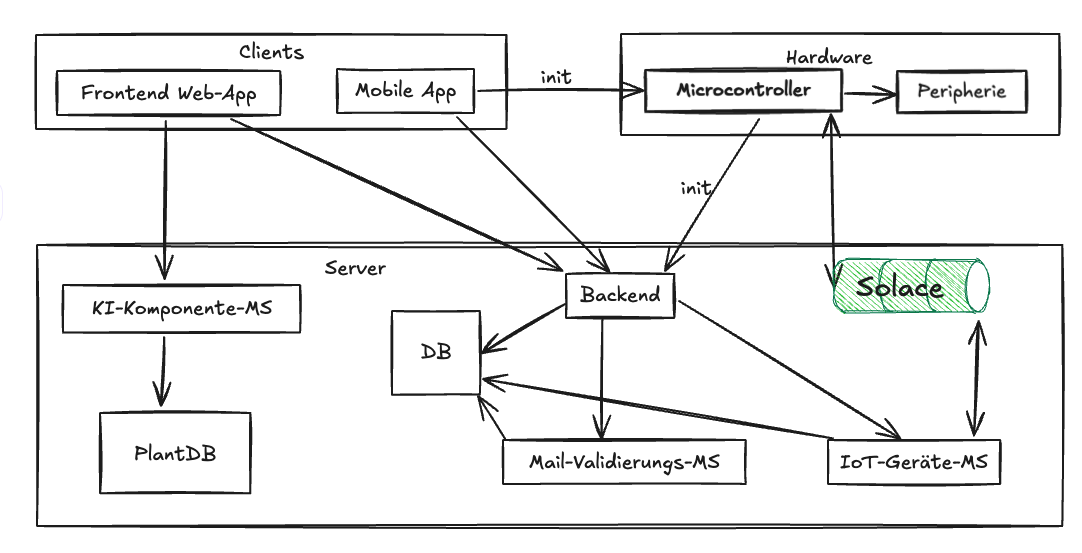
\includegraphics[scale=.35]{"./img/Kommunikation.png"}
	\caption{Kommunikation zwischen den Komponenten von Sensora}
	\label{fig:Kommunikation}
\end{figure}

\subsection{Hosting und Systemverbindungen}
Die Systemarchitektur der Anwendung basiert auf einem verteilten Ansatz, bei dem mehrere spezialisierte Komponenten zusammenwirken. Das Hosting erfolgt Docker basiert, wobei die Dienste in voneinander getrennten Containern betrieben werden. Diese Struktur ermöglicht eine hohe Skalierbarkeit und eine klare funktionale Trennung zwischen einzelnen Bereichen.
Zentraler Einstiegspunkt f"ur die NutzerInnen ist die Webanwendung bzw. die mobile App, welche beide als Client-Komponenten fungieren. Gew"ohnlich verl"aufen alle Anfragen dieser Clients über das zentrale Backend. Dieses bildet den Kern der Serverarchitektur und übernimmt die Koordination aller systemrelevanten Prozesse.
Eine Besonderheit stellt das Hinzufügen neuer Controller dar. In diesem Fall kommuniziert der Client direkt mit dem Mikrocontroller, um eine initiale Verbindung und Konfiguration zu ermöglichen. Diese Kommunikation ist notwendig, um die Geräte korrekt in das System einzubinden, bevor sie in den regulären Datenfluss übergehen.
Einige Komponenten wurden bewusst aus dem Haupt-Backend ausgelagert, um Zuständigkeiten zu trennen und das System modular zu halten. Dazu gehört unter anderem die Kommunikation mit den Mikrocontrollern, die über eine eventbasierte Architektur mithilfe des Nachrichtensystems \textit{Solace} realisiert wird. Dabei senden die Controller ihre Sensordaten nicht direkt an das Backend, sondern publizieren diese über Solace. Ein spezialisierter Microservice nimmt diese Nachrichten entgegen und verarbeitet sie asynchron weiter.
Auch die E-Mail-Verifikation sowie die Analyse durch die KI-Komponente sind eigenständige Microservices, die über interne APIs in das Gesamtsystem integriert sind. Dies erlaubt eine unabhängige Entwicklung und Wartung dieser Teilfunktionen ohne direkte Abhängigkeit vom Kernsystem.
Die Datenpersistenz erfolgt über eine zentrale Datenbank, welche alle benutzerbezogenen und systemkritischen Informationen verwaltet. Die KI-Komponente nutzt für ihre Analysen eine separate Datenbasis zur Speicherung pflanzenspezifischer Informationen.
Insgesamt ergibt sich ein flexibles, erweiterbares System, das sowohl unmittelbare Benutzerinteraktionen als auch zeitlich versetzte, datengesteuerte Prozesse unterstützt.

        \section{Frontendarchitektur und Datenflüsse im System}
Die Frontendarchitektur des smarten Bewässerungssystems wurde nach dem Paradigma komponentenbasierter Webentwicklung realisiert. Ziel war es, eine modular aufgebaute, wartbare und reaktive Benutzeroberfläche zu schaffen, die flexibel auf unterschiedliche Endgeräte und Benutzeranforderungen reagiert. Im Zentrum steht dabei das Framework Vue.js in Verbindung mit dem State-Management-Tool Pinia. Im Folgenden werden die Strukturierung der Views, das Datenflussmodell sowie die Rolle zentraler Technologien im Detail betrachtet.

\subsection{Komponentenbasierte Struktur und Navigationsmodell}
Die Architektur der vorliegenden Anwendung folgt einem komponentenbasierten Ansatz gemäß der Vue.js-Konventionen. Jede View in der Applikation ist als \ac{SFC} implementiert. Eine \ac{SFC} vereint die drei wesentlichen Bestandteile einer Webkomponente in einer Datei: Template, Script und Styles. Das Template definiert die Benutzeroberfläche in HTML-ähnlicher Syntax, das Script implementiert die zugehörige Logik (meist in TypeScript), und der Style-Block regelt das visuelle Layout mittels CSS bzw. Tailwind CSS. Diese Trennung innerhalb einer Datei fördert sowohl die Lesbarkeit als auch die Wiederverwendbarkeit von Komponenten \cite{VueGuide2024}.

Die Views der Anwendung (z. B.	\texttt{HomeView}, 	\texttt{SinglePlantView}, 	\texttt{GroupView}, 	\texttt{SingleSensorView} sowie 	\texttt{PlantListView}) stellen jeweils eigenständige Seiten dar, die durch den Einsatz des Vue Routers dynamisch geladen werden. Jede dieser Views aggregiert untergeordnete Komponenten wie Karten, Dialoge, Navigationsleisten oder Diagramme und bindet dabei die jeweils relevanten Daten aus dem zentralen Zustand.

Die Navigationsstruktur ist hierarchisch aufgebaut. Eine Hauptansicht (\texttt{HomeView}) dient als Einstiegspunkt und aggregiert Informationen aus den verschiedenen Kontexten: Räume, Pflanzen und deren Sensordaten. Ausgehend davon ermöglicht das Routing eine Tiefennavigation bis auf Objektebene, z.\,B. zum Bearbeiten einer bestimmten Pflanze. Dies fördert die kognitive Abbildung realweltlicher Strukturen (Wohnung $\rightarrow$ Raum $\rightarrow$ Pflanze) im digitalen Raum.
 
 \subsection{Pinia als Vermittlungsinstanz zwischen API und Frontend}
 Zur zentralen Zustandsverwaltung kommt Pinia zum Einsatz, welches das offizielle State-Management-System für Vue 3 darstellt \cite{Vuex, Allotey2023}. Anders als bei Vuex erfolgt die Definition eines Stores in Pinia mittels der Funktion \texttt{defineStore}, wobei sowohl State als auch Actions und Getters kapsuliert definiert werden. Diese Struktur unterstützt sowohl die Modularität als auch die Wiederverwendbarkeit der Zustandslogik.
 
 Pinia fungiert im Anwendungskontext als Puffer und vermittelnde Instanz zwischen dem Frontend und der REST-API. Die Stores agieren als Cache: sie speichern persistente Daten über Komponentenlebenszyklen hinweg und reduzieren dadurch die Anzahl notwendiger API-Anfragen. Dies verbessert sowohl die Performance als auch die Benutzererfahrung, da viele Interaktionen lokal bedient werden können. Persistiert wird der Zustand mittels \texttt{pinia-plugin-persistedstate} im \texttt{localStorage}, wodurch Informationen wie eingeloggte Nutzer oder selektierte Objekte auch bei einem Seitenreload erhalten bleiben.
 
 In der Applikation existieren getrennte Stores für Benutzerinformationen (\texttt{user.ts}), Authentifizierung (\texttt{auth.ts}), Pflanzen (\texttt{plant.ts}), Geräte (\texttt{device.ts}) und Räume (\texttt{room.ts}). Jeder Store definiert spezifische Actions, typischerweise asynchrone Methoden, alle die API-Schnittstellen repräsentieren und einige Weitere. Wenn Änderungen stattfinden, werden diese immer direkt an die API gesendet. Wenn Daten abgefragt werden, wird zuerst geprüft ob sie im Store verfügbar sind, wenn nicht wird erst eine Anfrage ans Backend gestellt. Diese neuen Daten werden dann gespeichert und automatisch in die andern Stores synchronisiert. 
 
 Optional kann eine Aktion auch mit einem \texttt{force}-Flag aufgerufen werden, welches eine explizite Aktualisierung erzwingt. Dies geschieht Beispielsweise bei "Pull-to-Refresh". Diese Strategie erlaubt einen kontrollierten Kompromiss zwischen Reaktivitiät und Ressourceneffizienz.
 
Um die Daten vor missbräuchlichen Zugriff zu schützen, wurde eine explizite Clear-Strategie implementiert. Bei Logout oder Benutzerwechsel werden alle Stores mittels \texttt{clearData()} zurückgesetzt, wodurch Persistenzdaten und Zustand explizit gelöscht werden. Das explizite Löschen ist auch über die Benutzereinstellung möglich.

\subsection{Datenfluss nach dem Flux-Prinzip}

Die Applikation folgt in ihrer Zustandslogik dem Flux-Prinzip, das ursprünglich von Facebook zur Beherrschung komplexer UI-Zustände vorgeschlagen wurde. Charakteristisch für dieses Architekturmodell ist ein strikt unidirektionaler Datenfluss: Interaktionen in der Benutzeroberfläche führen zu sogenannten Actions, die logische Operationen wie API-Aufrufe oder Validierungen auslösen. Die dabei gewonnenen Daten werden im zentralen State-Container gespeichert, welcher wiederum die View reaktiv aktualisiert. Dieser Ablauf lässt sich als Kette beschreiben: \texttt{UI $\rightarrow$ Action $\rightarrow$ Backend $\rightarrow$ Store $\rightarrow$ UI} \cite{Flux, facebook_flux}.

Die Trennung der Zuständigkeiten – insbesondere zwischen Anzeige, Logik und Datenhaltung – begünstigt eine konsistente und vorhersehbare Datenverwaltung. Da alle Zustandsveränderungen über dedizierte Actions verlaufen und sich zentral nachverfolgen lassen, verbessert das Modell sowohl die Testbarkeit als auch die Wartbarkeit der Anwendung \cite{Flux}. In Kombination mit Pinia, das als modernes, modulbasiertes State-Management-Tool agiert, ergibt sich eine Architektur, die eng an Flux angelehnt ist, dabei jedoch die Komplexität traditioneller Implementierungen (z.\,B. Redux) vermeidet.

 \subsection{Fazit}
 Die vorliegende Frontend-Architektur basiert auf einem robusten Zusammenspiel modularer Komponenten, zentralisiertem State-Management mit Pinia und asynchroner Datenkommunikation. Die Trennung von Zustandslogik und Darstellung, kombiniert mit der Persistenz und Synchronisationsstrategie, gewährleistet eine wartbare und benutzerfreundliche Applikation.
 
 
        \section{Benutzerzentriertes Design und UI/UX im Frontend}

Im Bezug auf die theoretische Erläuterung zentraler Konzepte wie \ac{UCD} und den Usability-Heuristiken nach Nielsen sowie dem \ac{UX}-Leitbild des Responsive Designs, wird in diesem Abschnitt die konkrete Umsetzung dieser Prinzipien im Rahmen der Vue.js-basierten Anwendung dargestellt. Ziel ist es, die Überführung theoretischer Vorgaben in praktische Gestaltungslösungen nachvollziehbar zu machen und zu zeigen, wie benutzerzentrierte Entwicklung zur Verbesserung der \ac{UI}-Qualität beiträgt.

\subsection{Anwendung von UCD im smarten Bewässerungssystem}

Die Nutzerforschung erfolgte durch halbstrukturierte Interviews mit VertreterInnen der Zielgruppe (z.\,B. HobbygärtnerInnen, technikaffine Personen). Daraus wurden mehrere Personas abgeleitet, die unterschiedliche Nutzungsmotive wie einfache Bedienung, Transparenz von Sensordaten und Kooperation abbilden. 

Darauf aufbauend wurden Wireframes auf Papier entwickelt, welche die Informationsarchitektur und zentrale Navigationsstrukturen skizzierten. Diese papierbasierten Modelle wurden iterativ angepasst und mit ausgewählten Testpersonen diskutiert. Durch diese formative Evaluation konnte bereits vor der Implementierung auf zentrale Anforderungen reagiert werden.

Auf Basis des Nutzerfeedbacks wurde die Darstellung der Gruppenansicht verbessert. Konkret ergaben sich folgende Anforderungen: Die NutzerInnen wünschten sich eine übersichtliche Darstellung der Gruppen sowie die Möglichkeit, auf einfache Weise die MitgliederInnen einer Gruppe einzusehen, ohne dass zu viele Informationen gleichzeitig auf dem Bildschirm erscheinen. Um diese Bedürfnisse zu erfüllen, wurde die GroupsView als Card-Layout konzipiert.

Diese Card präsentiert auf den ersten Blick nur die wichtigsten Informationen einer Gruppe. Über den Titel oder dem Button können die NutzerInnen die Card bei Bedarf „ausklappen“. Wird der Button gedrückt, erweitert sich die Card dynamisch und zeigt alle zugehörigen MitgliederInnen an. Dies verbessert die Übersichtlichkeit, da nicht alle Details permanent sichtbar sind und die NutzerInnen selbst steuern können, wann sie vertiefte Informationen einsehen.

Besonders benutzerfreundlich ist die neue Lösung auch darin, dass, wenn nur eine einzige Gruppe vorhanden ist, diese Card bereits automatisch ausgeklappt dargestellt wird. Auf diese Weise entfällt ein unnötiger zusätzlicher Klick und der direkte Zugriff auf die Gruppendetails wird erleichtert – ein kleines Detail, das jedoch signifikant zur Verbesserung der User Experience beiträgt.

Eine weitere Optimierung ist auf der SingelPlantView gemacht worden.
Aufgrund Nutzerfeedbacks wurde eine horizontale Linie in das Diagramm integriert, um den Sollwert des Messsatzes optisch darzustellen. Die Linie ermöglicht es den Nutzerinnen und Nutzern sofort zu erkennen, wo sich der Sollwert im Vergleich zu den aktuellen Messwerten befindet, sodass Abweichungen zwischen Soll- und Ist-Werten intuitiv nachvollziehbar werden. Dadurch wird nicht nur die Übersicht verbessert, sondern auch die Entscheidungsfindung optimiert, da eine klare visuelle Referenz bereitgestellt wird, anhand derer schneller und fundierter bestimmt werden kann, ob und in welchem Umfang eine Anpassung – beispielsweise im Bewässerungsprozess – erforderlich ist.

Durch die Integration der horizontalen Linie wird die Anwendung benutzerfreundlicher und nachvollziehbarer gestaltet. Gleichzeitig fügt sich die Linie nahtlos in das bestehende Design der SinglePlantView ein, das auf eine klare und konsistente Visualisierung von Daten setzt und damit zentrale Usability-Heuristiken wie die „Sichtbarkeit des Systemstatus“ sowie „Konsistenz und Standards“ unterstützt.


\subsection{Verwendete Heuristiken in der Anwendung}

Im Rahmen der konkreten Umsetzung wurden mehrere der zehn Usability-Heuristiken nach Nielsen gezielt berücksichtigt und systematisch in die Gestaltung der Benutzeroberfläche integriert:

Die Heuristik der Sichtbarkeit des Systemstatus wird durch die Verwendung von Toast-Notifications umgesetzt. Diese erscheinen automatisch bei allen Backend-Abfragen und informieren die NutzerInnen unmittelbar über den Verlauf und das Ergebnis einer Operation. Zusätzlich zeigen Statusindikatoren den Zustand des Sensors an.

Konsistenz und Standards werden durch den Einsatz von Tailwind CSS in Verbindung mit einheitlich definierten Designvariablen gewährleistet. Farben wie \texttt{primary}, \texttt{secondary}, \texttt{destructive} oder \texttt{background} kommen konsistent in Buttons, Karten und Formularen zum Einsatz und tragen zu einem kohärenten Erscheinungsbild bei \cite{TailwindCSS}.

Zur Umsetzung der Heuristik Fehlervorbeugung wurden alle Formulare mit clientseitiger Validierung ausgestattet. Eingaben werden bereits vor dem Absenden überprüft und Fehler mit Toast-Notifications angezeigt. Leere Eingabefelder enthalten stets einen Platzhalter, der die erwartete Eingabe beschreibt und so die korrekte Nutzung unterstützt.

Die Heuristik Hilfe und Dokumentation wurde durch einige kontextabhängige Tooltips sowie strukturierte Leere-Zustandsanzeigen berücksichtigt. Diese informieren über die nächsten Schritte oder ermöglichen eine direkte Navigation zur entsprechenden Aktion.

Ergänzend wurde auch die Heuristik Entsprechung zwischen System und realer Welt umgesetzt. Die hierarchische Struktur der Anwendung – von der Wohnung über Zimmer bis zu einzelnen Pflanzen – entspricht einem mentalen Modell aus dem Alltagskontext. Diese logische Ordnung fördert die Orientierung und trägt zu einer intuitiven Navigation bei.

Weitere Heuristiken wie Ästhetisches und minimalistisches Design sind durch das reduzierte Tailwind-basierte UI implizit realisiert worden.

Insgesamt zeigt sich, dass zentrale Usability-Prinzipien systematisch in das UI-Design integriert wurden, um eine benutzerfreundliche und robuste Anwendungserfahrung zu gewährleisten.

\subsection{Responsive Design}

Die Umsetzung des Responsive Designs wurde dabei so angelegt, dass die Anwendung unabhängig von der verwendeten Gerätegröße ein konsistentes und nutzerfreundliches Erlebnis bietet. Mithilfe der Tailwind-Breakpoints \texttt{sm}, \texttt{md}, \texttt{lg} und \texttt{xl} können Layout, Typografie und Abstände flexibel an kleinere, mittlere und größere Displays angepasst werden \cite{TailwindCSS}. Dies stellt sicher, dass die einzelnen Interface-Elemente, wie Buttons, Karten und Navigationsmenüs, sich dynamisch skalieren und neu anordnen, um eine optimale Lesbarkeit und Bedienbarkeit zu gewährleisten.

Für alle Gerätetypen wurde zudem eine Bottom-Navigation implementiert, die insbesondere auf mobilen Endgeräten eine intuitive und leicht zugängliche Navigation ermöglicht. Diese Navigation dient als zentrales Steuerelement, das es den NutzerInnen erlaubt, unkompliziert zwischen den Hauptbereichen der Anwendung zu wechseln, ohne auf aufwendige und unübersichtliche Menüstrukturen zurückgreifen zu müssen.

Ein weiteres Gestaltungselement ist das horizontale Scrollen auf der Startseite. Dieses Feature wurde eingeführt, um mehrere Informationskarten kompakt darzustellen, ohne dass der vertikale Platz unnötig beansprucht wird. Durch diese Anordnung können NutzerInnen schnell einen Überblick über verschiedene Inhalte erhalten und bei Bedarf mittels horizontaler Gesten zusätzliche Details abrufen. Insgesamt trägt das responsive Design dazu bei, dass die Anwendung sich flexibel an die individuellen Bedürfnisse und Nutzungsszenarien der AnwenderInnen anpasst und ein nahtloses Nutzungserlebnis über alle Geräte hinweg gewährleistet.

\subsection{User-Stories und funktionale Umsetzung}

Zur nutzerzentrierten Anforderungsdefinition wurden User-Stories eingesetzt, etwa:
\begin{itemize}
	\item \enquote{Als Benutzer möchte ich ein Pflanzenbild hochladen, damit die Pflanze automatisch erkannt wird.}
	\item \enquote{Als Benutzer möchte ich auch Mitglied anderer Gruppeen sein, um gemeinsam mit anderen NutzerInnen Pflanzen zu pflegen.}
\end{itemize}
Diese flossen in die Entwicklung dedizierter Komponenten ein (z.\,B. UploadPhotoView, GroupsView) und sicherten eine nutzergeleitete Gestaltung.

\section{Erweiterte Frontend-Techniken}
\label{sec:frontend-erweitert}

Im Folgenden werden ausgewählte Techniken vorgestellt, die in modernen Front\-end-Ar\-chi\-tek\-tur\-en zum Einsatz kommen. Einige dieser Methoden, wie Lazy Loading und Performance-Audits, wurden im Rahmen dieser Arbeit bereits angewendet. Andere Techniken, wie automatisierte Tests, werden exemplarisch vorgestellt, jedoch im Rahmen dieses \ac{POC} nicht implementiert.

\subsection{Lazy Loading in der Anwendung}

Zur Optimierung der initialen Ladezeit wurde in der entwickelten \ac{SPA} aktiv \emph{Lazy Loading} eingesetzt. Durch die dynamische Einbindung von Komponenten beim Navigieren zwischen Routen konnte die Bundle-Größe signifikant reduziert und die Interaktivität der Anwendung beschleunigt werden. 

Ein Beispiel für Lazy Loading stellt die dynamisch eingebundene Route zur Detailansicht einer Pflanze dar. Die zugehörige View \texttt{SinglePlantView.vue} wird erst bei tatsächlichem Aufruf geladen:

\begin{lstlisting}[caption=Lazy Loading per Route in Vue Router]
	routes: [
		{
			path: '/plant/:id',
			name: 'plantX',
			component: () => import('../views/SinglePlantView.vue'),
			meta: { requiresAuth: true, title: 'title.plant' },
		}
	]
\end{lstlisting}

Dieses Prinzip wurde konsistent auf alle Unterseiten angewendet. Der verwendete Build-Tool \emph{Vite} unterstützt dabei automatisch Code-Splitting und Tree Shaking, wodurch überflüssiger Code im Produktionsbuild entfernt wird \cite{ViteDocs2024,RollupDocs2024}.

\subsection{Frontend-Messung mit Lighthouse}

Zur Bewertung der Qualität der entwickelten Anwendung wurden regelmäßig \emph{Lighthouse-Audits} durchgeführt. Diese wurden in den Chrome Developer Tools erzeugt und analysierten zentrale Metriken wie \cite{GoogleLighthouse2024}:

\begin{itemize}
	\item \textbf{Performance:} First Contentful Paint, Time to Interactive, Speed Index
	\item \textbf{Accessibility:} Farbkontraste, semantische Struktur, ARIA-Rollen
	\item \textbf{Best Practices:} Ressourcennutzung, HTTPS
	\item  \textbf{SEO:}  Meta-Tags
\end{itemize}

Diese Angaben, wurden genutzt um stetig die Anwendung zu verbessern, gleich auch wenn bei einem \ac{POC} nicht der Schwerpunkt auf \ac{SEO} oder Accessability liegt. Die Performance wird auf den verschieden Seiten teilweise sehr unterschiedlich bewertet, da aber keine starken Verzögerungen bei der Bedienung identifiziert wurden, wurde keine allgemeine Optimierung durchgeführt.
	\section{Aufbau einer spezifischen View als Vertreter}
Die Datei \texttt{SinglePlantView.vue} bildet das Grundgerüst für die Detailansicht einer einzelnen Pflanze in. Diese View ist modular aufgebaut und umfasst mehrere miteinander koordinierte Komponenten, die sowohl funktional als auch visuell klar voneinander getrennt sind. Die Umsetzung folgt modernen Prinzipien komponentenbasierter Architektur in Vue, wobei jede logische Funktionseinheit in eine eigene Komponente oder ein strukturell abgegrenztes Template-Element eingebettet ist. Die Aufteilung in Subbereiche ergibt sich direkt aus den Bedürfnissen einer klaren Benutzerführung sowie der funktionalen Entkopplung von Darstellung und Logik. Eine Darstellung der kompletten Komponente ist in \vref{fig:SingelPlantView} zu sehen.

\begin{figure}[H]
	\centering
	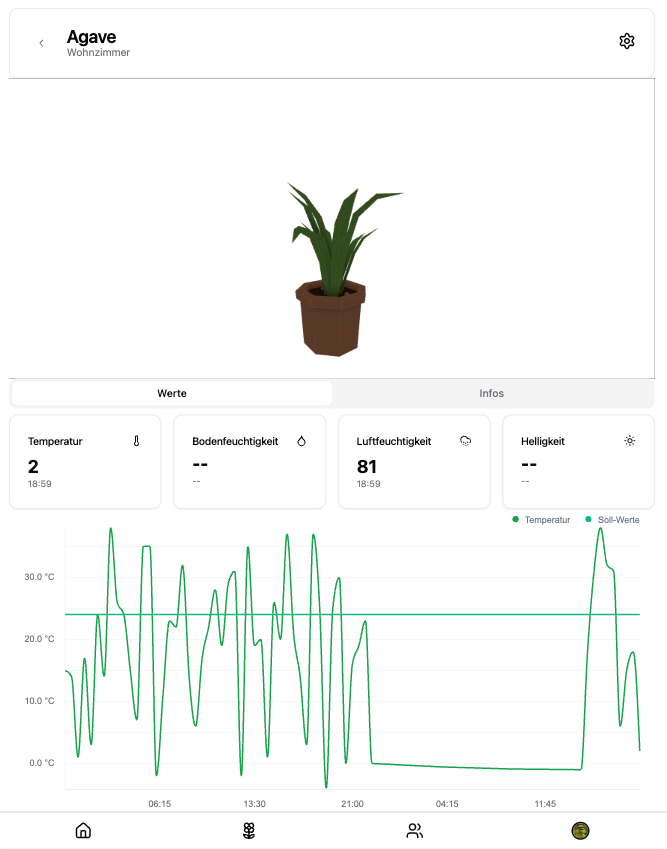
\includegraphics[scale=.5]{"./Umsetzung/images/sensora.png"}
	\caption{SinglePlantView in Aktion}
	\label{fig:SingelPlantView}
\end{figure}

Im oberen Abschnitt ist die Komponente \texttt{NavCard.vue} zu finden. Die ist für Überschriften mit einfacher Navigation zuständig in mehreren Views. Dieser Bereich ist durch die statische Anzeige des Pflanzennamens („Agave“) sowie der Rauminformation („Wohnzimmer“) gekennzeichnet. Diese Informationen werden direkt aus dem zentralen Datenmodell geladen, welches über ein Pinia-Store-Modul eingebunden ist. Der Benutzer erhält hier sofort kontextuelle Informationen zur Zuordnung der Pflanze im System.

Unmittelbar darunter befindet sich die 3D-Visualisierung der Pflanze, welche als zentrales visuelles Element prominent dargestellt ist. Diese Visualisierung basiert auf einem in der Datei \texttt{plantAvatars.ts} definierten Pflanzenmodell, das auf Basis des Pflanzentyps dynamisch geladen wird. Die Komponente zur Darstellung selbst ist als \texttt{<plant3d />} eingebettet, wobei ein Canvas-Rendering mit \texttt{Three.js} verwendet wird. Die visuelle Präsentation trägt zur Gamification der Anwendung bei, indem sie die emotionale Bindung und Wiedererkennung der Pflanzen fördern soll \cite{Werbach2012}.

Darunter folgt ein horizontal geteilter Abschnitt mit zwei Tabs: „Werte“ und „Infos“. Der Reiter „Werte“ ist standardmäßig aktiv, was sich in der visuellen Hervorhebung des Tabs zeigt. Innerhalb dieses Tabs sind vier Kartenkomponenten (Card-Komponenten) zu erkennen, die jeweils einen Umweltsensorwert repräsentieren: Temperatur, Bodenfeuchtigkeit, Luftfeuchtigkeit und Helligkeit. Diese sind als wiederverwendbare UI-Komponenten realisiert, die dynamisch Daten einlesen und anzeigen. Die Temperatur- und Luftfeuchtigkeitswerte sind im dargestellten Beispiel verfügbar („18 °C“ und „70 \%“), während Bodenfeuchte und Lichtstärke als nicht verfügbar („--“) markiert sind – ein Hinweis auf fehlerhafte oder fehlende Sensoranbindung. Jede Karte zeigt zusätzlich den letzten Messzeitpunkt, was eine präzise Einordnung der Datenqualität ermöglicht.

Der untere Teil der View wird durch die Verlaufsgraphen-Komponente dominiert, die in \texttt{PlantMeasuredValuesChart.vue} ausgelagert ist. Diese Komponente nutzt den Wrapper von \texttt{shadcn-vue} für \texttt{unovis}, um Messwerte über einen Zeitraum hinweg grafisch darzustellen. Im dargestellten Screenshot ist ein Temperaturliniendiagramm zu sehen, das über 24 Stunden  Werte anzeigt. Ein horizontaler Zielwert (Soll-Wert) ist ebenfalls dargestellt, was dem Benutzer eine sofortige Einschätzung der Umweltbedingungen erlaubt. Die Auswahl dieses Visualisierungsformats folgt dem Prinzip der kognitiven Entlastung: Durch einfache visuelle Kodierung können Zustände schneller interpretiert werden als durch numerische Tabellen.

Abgeschlossen wird die Komponente durch die \texttt{BottomNavBar.vue}, die über vier Icons eine einfache Navigation innerhalb der Anwendung ermöglicht. Diese sind als feste UI-Komponenten realisiert, wobei ein Button speziell dem Rücksprung zur Pflanzenübersicht oder der Startseite dient.

Insgesamt ergibt sich aus dieser strukturierten Aufteilung ein konsistentes, nutzerzentriertes Interface, das sowohl eine einfache Übersicht als auch eine tiefgehende Analyse einzelner Pflanzendaten erlaubt. Die klare funktionale Trennung – Datenanzeige oben, Visualisierung unten, Navigation ganz unten – folgt bewährten Usability-Prinzipien, die sich in wissenschaftlicher Literatur zur Mensch-Computer-Interaktion vielfach bewährt haben \cite{norman2013design}.



        \section{KI-Komponente zur automatisierten Pflanzenklassifikation}
Ziel dieses Moduls war der Aufbau eines robusten Deep-Learning-Modells zur Klassifikation von Pflanzenarten anhand fotografischer Bilddaten. Als Datengrundlage diente der PlantNet-300K-Datensatz, ein umfassender, realweltlicher Datensatz, der über 300.000 Pflanzenbilder aus verschiedenen Regionen und Perspektiven umfasst \cite{Affouard2017}. Der Ausgangsdatensatz enthielt über 1.000 Pflanzenklassen, wobei ein starker Klassenunterschied hinsichtlich der Bildanzahl pro Klasse vorlag – von 1 Bildern bis zu über 5.000 Bildern pro Art. Um ein Mindestmaß an statistischer Repräsentation zu gewährleisten und extreme Ausreißerklassen zu vermeiden, wurden für das Training ausschließlich Klassen berücksichtigt, die mindestens 5 Bilder enthielten. Diese Filterung reduzierte das Klassenspektrum auf 837 distinkte Pflanzenarten.
Diese Klassen besteht zum Großteils aus nicht sehr verbreiteten Pflanzen in Deutschland.

\subsection{Modellarchitektur und Trainingsstrategie}

Die Trainingspipeline basiert vollständig auf einem vortrainierten \ac{ResNet50}-Modell, das von Beginn an zur Initialisierung genutzt wurde. Die Wahl von \ac{ResNet50} ergibt sich aus mehreren architektonischen und empirisch belegten Vorteilen: \ac{ResNet} wurde eingeführt, um ein zentrales Problem tiefer neuronaler Netze zu adressieren – das sogenannte \emph{Degradationsproblem}. Dabei nimmt bei tiefer werdenden Netzen nicht nur die Trainingszeit zu, sondern mitunter sogar die Klassifikationsleistung ab, obwohl das Netz mehr Kapazität besitzt \cite{He2015}.

Der Kernmechanismus zur Lösung dieses Problems sind \emph{Residual-Blöcke}. Statt rohe Ausgaben direkt weiterzureichen, lernen ResNet-Blöcke nur die Abweichung von der Identität\cite{He2015}.

Das \ac{ResNet50}-Modell besteht aus insgesamt 50 Schichten, die sich aufteilen in:
\begin{itemize}
	\item eine initiale Convolution-Schicht (7x7 Convolution + MaxPooling),
	\item 16 sogenannte „Bottleneck“-Blöcke mit je drei Schichten (1x1 $\rightarrow$ 3x3 $\rightarrow$ 1x1 Convolution),
	\item Batch-Normalisierung und ReLU-Aktivierung in jedem Block,
	\item eine globale Average-Pooling-Schicht,
	\item sowie eine abschließende Fully-Connected-Schicht zur Klassifikation.
\end{itemize}

Durch diese Struktur ist \ac{ResNet50} nicht nur leistungsfähig, sondern auch besonders übertragbar auf neue Datendomänen – ein Umstand, der in einer Vielzahl an Transfer-Learning-Studien belegt wurde \cite{Kornblith2019}. Die Tiefe erlaubt es dem Modell, auch feine, visuell komplexe Unterschiede zwischen Pflanzenarten zu modellieren, während die Sprungverbindungen die Stabilität im Training erhalten.

 Im initialen Training wurden alle Schichten des Netzwerks feinjustiert. Nach einer ersten Konvergenz wurde ein Finetuning durchgeführt, bei dem ein Großteil der Layer eingefroren wurde, um ausschließlich die letzten Klassifikationsschichten anzupassen. Dieses zweistufige Vorgehen ist ein gängiger Transfer-Learning-Ansatz, insbesondere wenn ein großes Ausgangsmodell (wie \ac{ResNet}) auf eine domänenspezifische Aufgabe adaptiert wird \cite{Pan2010}.

\subsection{Regularisierung und Datenkonsolidierung}
Zur Verbesserung der Modellrobustheit wurden mehrere datenaugmentierende Verfahren eingesetzt. Dazu zählen insbesondere Mixup \cite{Zhang2018} und CutMix \cite{Yun2019}, welche zu besseren Verallgemeinerungseigenschaften führen, indem sie die Entscheidungsgrenzen im Merkmalsraum glätten. Ergänzt wurden diese Verfahren durch RandAugment, eine robuste Augmentierungsmethode ohne komplexe Hyperparametrierung.

Ein zentrales Vorverarbeitungsschritt war die Anwendung des Moduls \file{\url{create\_merge\_ map.py}}, das vor dem Finetuning genutzt wurde, um Duplikate und taxonomisch redundante Pflanzenklassen zusammenzuführen. Diese Maßnahme reduziert das Risiko semantischer Verwirrung im Trainingsprozess und wurde insbesondere bei identischen oder sehr ähnlichen Arten eingesetzt. Die Notwendigkeit solcher Label-Konsolidierungen ist insbesondere in crowd-basierten, multilinguistisch annotierten Datensätzen wie PlantNet belegt \cite{Horn2018}.

Darüber hinaus wurde zur Kompensation des hochgradig unausgeglichenen Klassenverhältnisses (5–5000 Bilder pro Klasse) ein Weighted Sampling implementiert. Diese Technik erhöht die Wahrscheinlichkeit der Auswahl von Bildern seltener Klassen während des Batch-Trainings und verhindert so die Dominanz überrepräsentierter Arten im Gradientenfluss – ein gängiger Ansatz zur Balancierung von Imbalancen in Klassifikationsaufgaben \cite{Buda2018}.

\subsection{Leistung und Interpretation}

Die Trainingszeit betrug insgesamt 65 Stunden, wobei 50 Stunden auf das initiale, vollständig entfrorene Training und 15 Stunden auf das anschließende Finetuning entfielen.

Das finale Modell demonstrierte eine hohe Klassifikationsfähigkeiten. Die Top-1-Accuracy von 77\% bedeutet, dass das Modell in über drei Viertel aller Fälle die exakte Pflanzenart korrekt identifizierte. Die Top-5-Accuracy von 95\% zeigt, dass sich die wahre Klasse in der Mehrheit der Fälle unter den fünf wahrscheinlichsten Vorhersagen befand – ein Maß, das insbesondere in praktischen Anwendungen wie botanischen Bestimmungs-Apps von Relevanz ist. In der Abbildung \vref{fig:plantAI} sind Beispiel zu sehen.

\begin{figure}[H]
	\centering
	
	% Erste Zeile
	\begin{minipage}[t]{0.40\textwidth}
		\centering
		\includegraphics[angle=-90, width=\linewidth]{./Umsetzung/images/1.jpg}
		\caption{Korrekt erkannt als Anthurium Andraeanum mit 99,72\%}
	\end{minipage}
	\hfill
	\begin{minipage}[t]{0.40\textwidth}
		\centering
		\includegraphics[angle=-90, width=\linewidth]{./Umsetzung/images/2.jpg}
		\caption{Korrekt erkannt als Fragaria X Ananassa mit 90,42\%}
	\end{minipage}
	
	\vspace{0.3em}
	\begin{minipage}{\textwidth}
		\centering
		\small Abbildung oben: Übersicht einiger markanter Testpflanzen.
	\end{minipage}
	
	\vspace{1em}
	
	% Zweite Zeile
	\begin{minipage}[t]{0.40\textwidth}
		\centering
		\includegraphics[angle=-90, width=\linewidth]{./Umsetzung/images/3.jpg}
		\caption{Korrekt erkannt als Lavandula Stoechas mit 99,49\%}
	\end{minipage}
	\hfill
	\begin{minipage}[t]{0.40\textwidth}
		\centering
		\includegraphics[angle=-90, width=\linewidth]{./Umsetzung/images/4.jpg}
		\caption{Korrekt erkannt als Lavandula Angustifolia mit 98,05\%}
	\end{minipage}
	
	\vspace{0.3em}
	\begin{minipage}{\textwidth}
		\centering
		\small Abbildung unten: Vergleich der Genauigkeit zweier Lavendel Arten
	\end{minipage}
	
	\caption{Beispiel für die KI-Erkennung}
	\label{fig:plantAI}
\end{figure}



\subsection{Rolle der KI-Komponente bei der Pflanzenerstellung}

Die KI-Komponente wird im Gesamtsystem insbesondere bei der Erstellung neuer Pflanzeninstanzen eingesetzt. NutzerInnen haben dabei die Möglichkeit, grundlegende Eigenschaften einer Pflanze – wie den Pflanzennamen oder die Artzugehörigkeit – automatisiert durch ein KI-Modul bestimmen zu lassen. Dieser Vorgang kann sowohl durch das Hochladen eines bestehenden Pflanzenbilds als auch direkt über eine Fotoaufnahme im Browser oder auf mobilen Endgeräten ausgelöst werden. Alternativ besteht die Möglichkeit, ohne KI-Unterstützung nach einer Pflanze zu suchen.

Bei Nutzung der KI-Komponente wird das Bild über das Frontend an einen dedizierten Klassifikationsservice übermittelt. Dieser führt eine Inferenz mit dem trainierten \ac{ResNet50}-Modell durch und schlägt basierend auf der Bildanalyse eine Pflanzenart vor. Neben der wahrscheinlichsten Klasse wird zusätzlich eine Liste mit weiteren möglichen Arten inklusive Vorhersagewahrscheinlichkeiten generiert. Es werden aber nur Pflanzen mit über 50\% zurückgegeben. Diese Vorhersage wird visuell im Interface dargestellt und kann von der NutzerIn  bestätigt werden.

Der ausgewählte Vorschlag bildet dann die Grundlage für die Vorbelegung der Eingabefelder zur Pflanzenerstellung, sodass beispielsweise der wissenschaftliche Name, die Spezies und Soll-Werte geschätzt werden. Die KI-Komponente unterstützt somit aktiv die Datenerfassung und sorgt für eine beschleunigte, komfortable Erstellung von Pflanzendatensätzen innerhalb des Systems. Die finale Entscheidung über die Auswahl der vorgeschlagenen Pflanze verbleibt stets bei den Nutzenden.


	\section{Beschreibung des Datenbankaufbaus}
Die Datenbank des Systems Sensora ist im Schema sensora organisiert und verfolgt eine klar strukturierte, relationale Modellierung mit durchdachter Referentialität und Typisierung. Sie unterstützt die zentralen Funktionen des Systems wie Benutzerverwaltung, Gruppenzugehörigkeit, Raum- und Pflanzenzuordnung sowie Sensor- und Steuerdaten.
\newpage
\begin{figure}[H]
\centering
%  \includesvg[width=\linewidth, height=0.9\textheight, keepaspectratio,inkscapelatex=false]{img/Datenbank Diagramm.svg}
  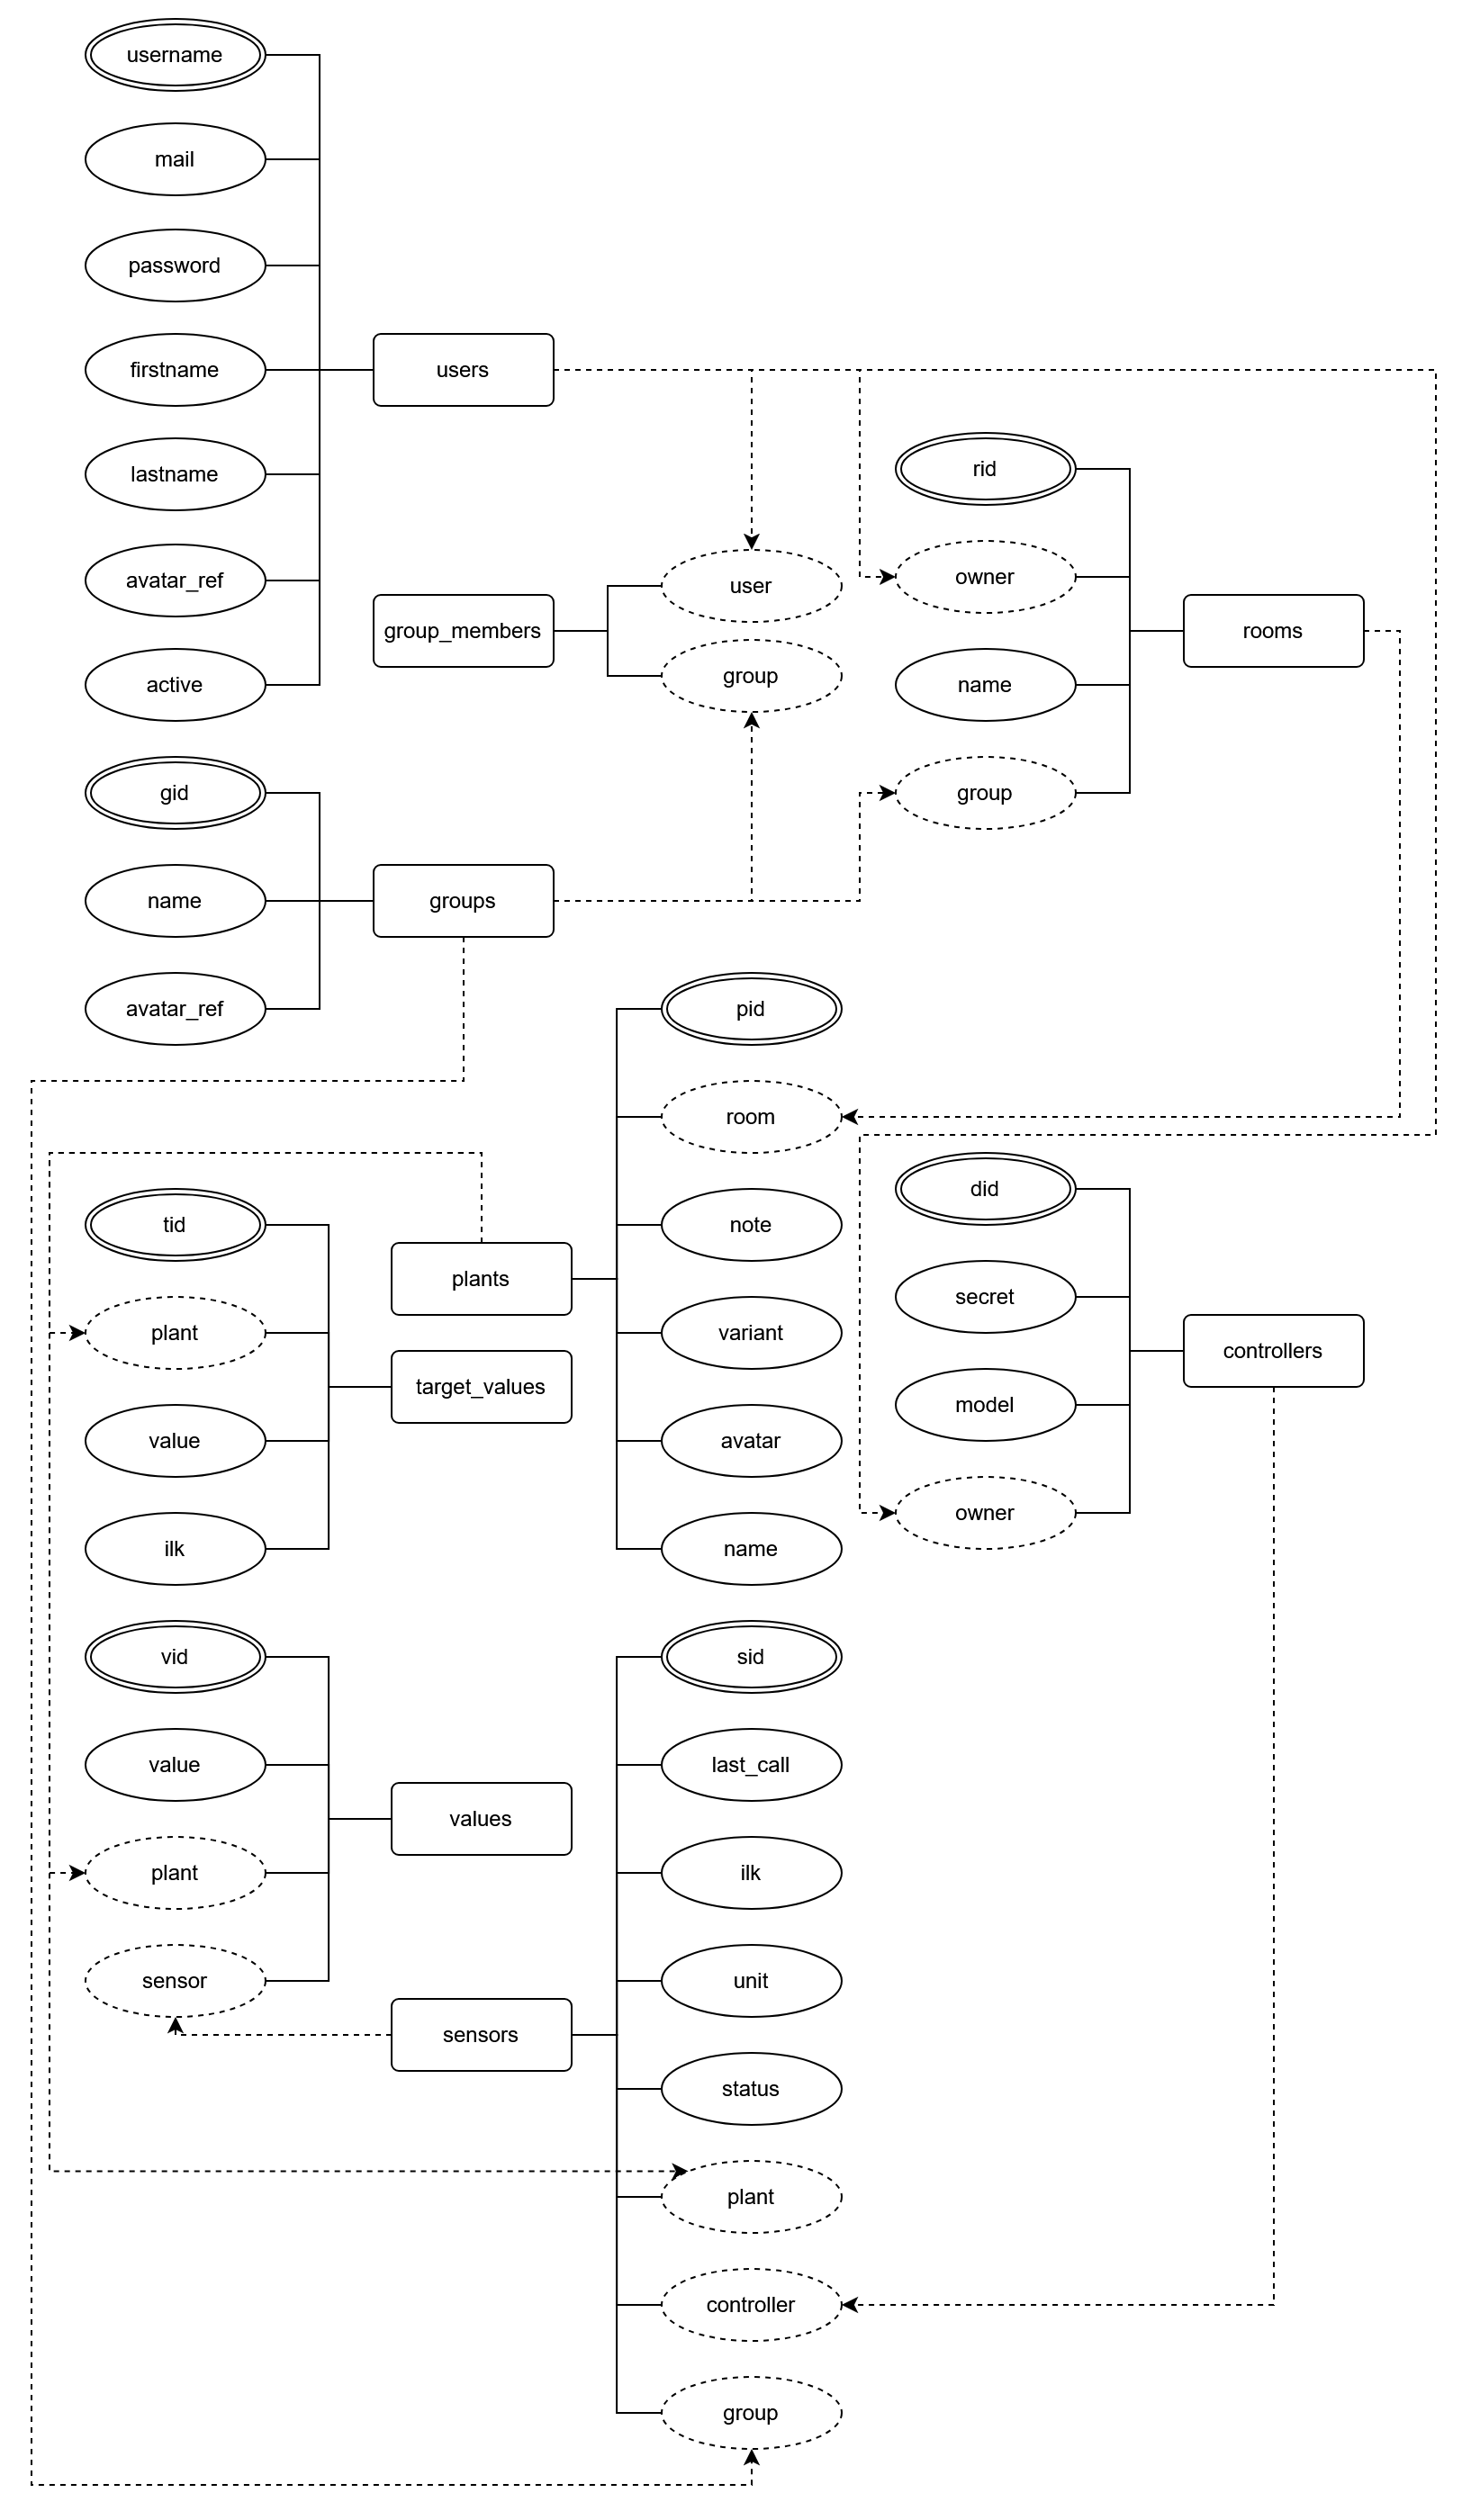
\includegraphics[width=\linewidth, height=0.9\textheight]{img/Datenbank Diagramm.png}
\caption{Sensora Datenbank Struktur}
\label{fig:sensora_datenbank}
\end{figure}
\newpage

\subsection{Struktur und Besonderheiten}
\begin{description}
    \item[Benutzerverwaltung:]
    Die Tabelle users bildet die zentrale Entität für Benutzer ab. Jeder Benutzer besitzt Pflichtangaben sowie einen referenzierten Avatar aus dem dedizierten ENUM-Typ sensora.avatar. Die E-Mail-Adresse ist eindeutig.
    \item[Gruppen \& Mitgliedschaften:]
    Gruppen (groups) können mehrere Mitglieder haben, realisiert durch die Join-Tabelle group\_members. Diese bildet eine klassische Many-to-Many-Beziehung zwischen Nutzern und Gruppen ab.
    \item[Räume \& Pflanzen:]
    Räume (rooms) können Gruppen zugeordnet sein und besitzen jeweils einen Eigentümer. Pflanzen (plants) sind immer einem Raum zugeordnet und dienen als Ankerpunkt für Messwerte.
    \item [Sensorik \& Steuerung:]
    Sensoren (sensors) sind mit Controllern (controllers) verknüpft und optional direkt mit einer Pflanze oder Gruppe verbunden. Jeder Sensor verwendet den ENUM-Typ sensora.status, um seinen Zustand zu klassifizieren.
    \item [Zielwerte \& Messdaten:]
    Pflanzen können über target\_values Zielgrößen definieren. Tatsächliche Messwerte werden in der Tabelle values gespeichert und jeweils einem Sensor sowie einer Pflanze zugeordnet.
\end{description}

\subsection{Technische Merkmale}
\begin{itemize}
    \item Es kommen ENUM-Typen zum Einsatz, um Felder wie Avatar und Status typensicher und standardisiert zu definieren.
    \item Sämtliche Fremdschlüsselbeziehungen nutzen CASCADE-Strategien zur Pflege von Konsistenz (z.B. beim Löschen von Benutzern oder Pflanzen).
    \item Indizes auf eindeutige Felder (z.B. mail, secret) erhöhen die Performanz gezielter Abfragen.
    \item Die Nutzung von Timestamps mit Standardwerten erlaubt eine automatische Protokollierung von Ereignissen wie Sensoraktivität.
\end{itemize}

Diese Datenbankstruktur ermöglicht eine flexible, erweiterbare und gleichzeitig robuste Grundlage für die Backend-Logik und garantiert eine nachvollziehbare Abbildung der fachlichen Entitäten.
        \section{Auth-Service: Geräteregistrierung und HMAC-Authentifizierung}
Der Auth-Service implementiert die sichere Registrierung und Anmeldung von Controllern mittels eines Challenge-Response-Verfahrens auf Basis eines vorab geteilten Geheimnisses (PSK). Dieser Dienst ist als Flask-Webanwendung realisiert und stellt HTTP-Routen für die Controller-Initialisierung, -Verifikation sowie eine Admin-Registrierung bereit. Er bildet damit das sicherheitskritische Bindeglied zwischen neuen Geräten und der Systeminfrastruktur: 
Geräte erhalten hier ihre individuellen Messaging-Zugangsdaten, sofern sie einen kryptographischen Besitznachweis erbringen. Im Folgenden werden die Architektur und der Ablauf des Auth-Service beschrieben, gefolgt von besonderen Implementierungsdetails wie der PSK-Überprüfung, Wiederanlaufbarkeit und der automatischen Broker-Konfiguration.
\subsection{Architektur und persistente Datenhaltung}
Der Auth-Service ist als Flask-Applikation mit dokumentierter REST-API (via Swagger/Flasgger) umgesetzt. Kern der Implementierung ist eine zentrale Konfigurationsdatei (auth\_config.json), die folgende Informationen persistent speichert:

\begin{enumerate}
    \item Authorized Controllers: eine Liste aller registrierten Controller mit deren Controller-ID (eindeutige Kennung), zugehörigem PSK (token) sowie einem Hash dieses Tokens (token\_hash). Zusätzlich werden Metadaten wie Modell, Besitzer (Benutzername) und Beschreibung gespeichert. Diese Datei dient als kleine lokale Datenbank, um bereits registrierte Geräte und ihre Geheimnisse nachzuhalten.
    \item Active Challenges: temporäre Herausforderungen (Challenges) im laufenden Authentifizierungsprozess.
    Für jeden angeforderten Auth-Vorgang wird ein zufälliger Challenge-String erzeugt und unter dem Schlüssel des token\_hash zwischengespeichert.
    Dies ermöglicht es, eingehende Antworten eindeutig der zuvor ausgegebenen Challenge zuzuordnen, selbst bei parallelen Anfragen.
    \item Solace Credentials: bereits für Controller erstellte Zugangs-Credentials für den Message Broker (Solace). Pro Gerät wird hier der erzeugte Broker-Benutzername und das Passwort abgelegt, um bei wiederholter Authentifizierung nicht erneut einen Broker-Account anlegen zu müssen.
\end{enumerate}
Die Konfigurationsdaten werden auf dem Container-Dateisystem unter /config/auth\_config.json verwaltet und durch Volume-Mounting persistent gehalten. Dadurch bleiben Registrierung und vergebene Credentials auch beim Neustart des Dienstes erhalten – ein wesentlicher Aspekt für Wiederanlaufbarkeit. Ergänzend hält der Auth-Service eine Datenbankverbindung (PostgreSQL via psycopg2) bereit, um neue Controller auch in der zentralen Systemdatenbank (sensora) zu registrieren. In der Tabelle sensora.controllers werden u.a. Device-ID, Modell, Besitzer und ein vom System generierter geheimer Schlüssel abgelegt. Letzterer unterscheidet sich vom PSK und dient ggf. anderen Zwecken (z.B. der Kommunikation mit externen Anwendungen), ohne das eigentliche PSK offenzulegen. Die doppelte Ablage (Datei und DB) der Registrierungsdaten mag auf den ersten Blick redundant erscheinen, ermöglicht jedoch sowohl schnelle lokale Zugriffe während des Auth-Handshakes als auch die Integration ins relationale Gesamtdatenmodell.

\subsection{Ablauf der Geräte-Registrierung und Authentifizierung}
Der Auth-Service bietet drei Haupt-Endpoints, die den Lebenszyklus eines Geräts abbilden: (a) Registrierung eines neuen Controllers (nur Admin), (b) Initialisierung des Authentifizierungs-Handshakes durch das Gerät und (c) Verifikation der Challenge-Response. 

Der Authentifizierungsablauf erfolgt in mehreren Schritten:
\begin{enumerate}
    \item Admin-Registrierung: Zunächst muss ein neuer Controller in das System aufgenommen werden. Ein Administrator (oder ein automatisierter Setup-Prozess) ruft dazu den Endpoint /api/admin/controller auf und übermittelt zumindest den gewünschten Besitzer (username) sowie optional eine vorgegebene Controller-ID und Modellbeschreibung. Der Request ist durch einen speziellen Admin-API-Key (Header X-Admin-Key) geschützt, sodass nur berechtigte Instanzen Geräte hinzufügen können. Bei Aufruf generiert der Service serverseitig ein zufälliges Token (PSK) für das Gerät (hier als UUID v4). Zusätzlich wird ein Token-Hash berechnet: mittels HMAC-SHA256 über das Token mit einem globalen Server-Geheimnis (TOKEN\_SECRET). Dieser Hash dient als öffentlicher Identifikator des Geräts, der das eigentliche Token nicht preisgibt. Anschließend werden die Gerätedaten in der auth\_config.json persistiert (authorized\_controllers) und ein Eintrag in der DB-Tabelle controllers erzeugt. Der Response an den Admin enthält Controller-ID, Token und Token-Hash, welche sicher an das Gerät für die Inbetriebnahme weitergegeben werden (z.B. manuell oder per Provisioning-App). Dieser einmalige Out-of-Band-Schritt stellt sicher, dass jedes Gerät ein individuelles geheimes Token besitzt, das dem Server bekannt ist.
    \item Challenge-Anforderung (Gerät → Auth-Service): Hat das Gerät vom Admin sein Token erhalten und wird erstmals online genommen, initiiert es den Authentifizierungsprozess über den Endpoint /api/controller/init. Dabei sendet das Gerät nur den Hash seines Tokens (token\_hash) im Request – das eigentliche Token bleibt geheim und wird nie direkt übertragen. Der Auth-Service prüft den Request und generiert eine kryptographisch zufällige Challenge (16 Byte Hex-String via secrets.token\_hex) als Antwort. Diese Challenge wird im Server-Konfigurationsspeicher unter active\_challenges zusammen mit einem Zeitstempel abgelegt, indiziert durch den token\_hash. Die Response an das Gerät enthält die Challenge als JSON. Aus Sicherheitsgründen findet an dieser Stelle noch keine Verifizierung statt – auch ein unbekannter Token-Hash erhält (vorläufig) eine Challenge. Der eigentliche Abgleich erfolgt erst im nächsten Schritt. Dieses zweistufige Verfahren erhöht die Sicherheit, da ein Angreifer ohne Besitz des PSK aus der Challenge alleine keinen Zugang erlangt. Wichtig ist, dass jede Challenge unvorhersehbar und einmalig ist, um Replay-Angriffe auszuschließen. Der Auth-Service stellt dies durch Verwendung eines Kryptografie-Moduls sicher (Python secrets \cite{pythonSecrets} bietet laut Dokumentation einen sicheren Zufallszahlengenerator für solche Token).
    \item Challenge-Response (Gerät → Auth-Service): Nach Erhalt der Challenge berechnet das Gerät die Antwort: Es verwendet sein geheimes Token und wendet darauf die gleiche Hash-Funktion an, die auch der Server kennt. Im Code wird dazu HMAC-SHA256 genutzt, wobei das Token als Schlüssel und der Challenge-String als Nachricht dient. Das Ergebnis ist die Challenge-Response (Hex-String). Diese Antwort schickt das Gerät zurück an den Auth-Service, zusammen mit seinem token\_hash (zur Identifikation der Challenge) und meist einem Benutzernamen oder Kontoinformationen des Eigentümers. Der Auth-Service schlägt nun in seiner Konfiguration den Eintrag zum token\_hash nach: Dort findet er das ursprünglich registrierte Token (PSK) und die zugehörige Controller-ID. Sollte kein Eintrag existieren, wird der Prozess abgebrochen – das Gerät war nie registriert oder der Hash unbekannt (Fehler 403). Andernfalls vergleicht der Server die vom Gerät gesendete HMAC-Antwort mit dem erwarteten Wert, den er selbst berechnet (hmac.compare\_digest() verhindert Timing-Angriffe bei der String-Bewertung). Stimmen Response und eigener Wert überein, ist bewiesen, dass das Gerät das geheime Token besitzt und somit authentisch ist. Dieses Challenge-Response-Verfahren stellt eine sichere Authentifizierung dar\cite{hmacRFC}, ohne das PSK selbst über das Netzwerk zu senden. Ein abgehörter Challenge/Response-Wert kann später nicht wiederverwendet werden, da bei der nächsten Anmeldung eine andere Challenge zum Einsatz kommt (kein statisches Passwort)
    \item Broker-Zugangsdaten erstellen: Nach erfolgreicher Verifizierung entfernt der Auth-Service die verwendete Challenge (Verbrauch der einmaligen Challenge) und fährt mit der Provisionierung des Geräts für das Messaging-System fort. Hier greift eine weitere wichtige Implementierungsentscheidung: Der Service konfiguriert den Solace-MQTT-Broker dynamisch über dessen Management-API (SEMP v2). Konkret wird geprüft, ob für den Controller bereits Broker-Zugangsdaten in solace\_credentials vorliegen. Ist dies der erste erfolgreiche Auth-Vorgang für dieses Gerät, generiert der Service mittels der Hilfsfunktion create\_solace\_user(controller\_id) einen dedizierten Broker-Account:
    \begin{enumerate}
        \item Es wird ein eindeutiger Client-Username für den Controller erstellt (z.B. controller\_ab12... gekürzt auf Basis der ID) und ein zufälliges Passwort (secrets.token\_urlsafe(32)).
        \item Für feingranulare Zugriffskontrolle richtet der Service ein eigenes ACL-Profil auf dem Broker ein. Dies geschieht über HTTP-Aufrufe an die SEMPv2-Konfigurationsschnittstelle des Solace-Brokers. Das ACL-Profil für den Controller erlaubt ausschließlich die für diesen Anwendungsfall nötigen Operationen:
        \begin{enumerate}
            \item Publish-Erlaubnis: Das Gerät darf nur auf seinem eigenen Topic-Pfad Messwerte publizieren. Im Prototoll wird das Topic-Muster sensora/v1/send/{controller\_id} verwendet. Über SEMP wird ein Topic Exception hinzugefügt, die genau dieses Topic für Publish freigibt (alle anderen werden per Default “disallow” gesetzt).
            \item Subscribe-Erlaubnis: Analog erhält das Gerät das Recht, Sollwert-Nachrichten zu abonnieren, die an sein spezifisches Target-Topic gesendet werden. Dies ist typischerweise sensora/v1/receive/{controller\_id}/targetValues. Auch hierfür wird programmgesteuert eine Ausnahme im ACL-Profil hinterlegt. Damit ist sichergestellt, dass der Controller nur Nachrichten empfängt, die explizit an ihn adressiert sind (und z.B. keine fremden Gerätedaten).
        \end{enumerate}
        \item Nachdem ACL-Profil und Berechtigungen erfolgreich angelegt wurden, erstellt der Service über die SEMP-API den Broker-Client-User und weist ihm dieses ACL-Profil zu. Sollte einer der Schritte fehlschlagen (z.B. aufgrund bereits existierender Einträge oder Verbindungsfehler zum Broker), bricht die Funktion ab und der Auth-Vorgang resultiert in einem Server-Fehler (HTTP 500). Im Erfolgsfall erhält der Auth-Service nun ein Credential-Paket bestehend aus Broker-URL, Username und Passwort für den neuen Controller.
    \end{enumerate}
    Die Nutzung der Solace Element Management Protocol API ermöglicht es, die Broker-Konfiguration zu automatisieren. Solace SEMP ist eine RESTful-Schnittstelle\cite{SolaceSEMP}, die das Anlegen von Objekten (Queues, Benutzer, ACLs etc.) per Skript erlaubt. Dadurch wird eine dynamische Inbetriebnahme neuer Geräte ohne manuelle Eingriffe möglich – ein wichtiger Vorteil im IoT-Kontext. Durch entsprechende Fehlerbehandlung (Auswerten des HTTP-Status: 200 Erfolg, 409 „Conflict“ bei bereits vorhandenen Ressourcen) ist die Funktion weitgehend wiederholbar, ohne Inkonsistenzen zu erzeugen. Beispielsweise würde ein erneuter Aufruf für denselben Controller erkennen, dass dessen Benutzerkonto schon existiert (der Auth-Service speichert dies ja auch in seiner config) und überspringt die Neuanlage. So bleibt der Prozess idempotent und ein Gerät könnte die Authentifizierung bei Bedarf erneut durchlaufen, um z.B. verlorene Credentials abzurufen.
    \item Registrierung abschließen und Antwort an Gerät: Zum Abschluss der /verify-Route führt der Auth-Service noch zwei Aktionen aus: (a) Eintrag in der Systemdatenbank: Falls noch nicht geschehen, wird der Controller endgültig in der sensora.controllers-Tabelle der DB vermerkt (inkl. Besitzverknüpfung zum Benutzerkonto, was zuvor im Request mitgesendet wurde). Außerdem kann hier optional ein Default-Sensor für den Controller in der DB angelegt werden (im Code wird bspw. ein Platzhalter-Sensor für Temperatur erstellt, um direkt Messwerte speichern zu können). (b) Secure Credential Delivery: Die vom Broker erzeugten Verbindungsdaten (Username/Passwort, Host) müssen nun dem Gerät mitgeteilt werden. Da diese Angaben sehr sensitiv sind, wurden besondere Maßnahmen getroffen, um sie vertraulich und integer zum Gerät zu übertragen. Der Server generiert zunächst einen einmaligen Session Key (eine randomisierte Byte-Sequenz mittels Fernet.generate\_key()), mit dem er die Credentials symmetrisch verschlüsselt (Fernet nutzt intern AES-128 in GCM-Modus\cite{fernetSpec} mit eingebauter HMAC für Integrität). Die so entstehende Ciphertext-Nutzlast wird als encrypted\_credentials bereitgestellt. Zusätzlich erzeugt der Server einen Credential-HMAC (credential\_key), indem er den Session Key mit dem ursprünglichen Geräte-PSK mittels HMAC-SHA256 signiert. Anschließend sendet der Auth-Service dem Gerät folgende Daten im JSON-Response:
    \begin{enumerate}
        \item session\_key: der im Base64-Format kodierte symmetrische Schlüssel,
        \item credential\_key: der HMAC (Hex-String) zur Absicherung,
        \item encrypted\_credentials: die verschlüsselten Broker-Zugangsdaten (Base64-Text).
    \end{enumerate}
    Diese Konstruktion erlaubt es dem Gerät, die erhaltenen Credentials auf Vertrauenswürdigkeit zu prüfen: Nur wenn es den gleichen HMAC über den Session Key mit seinem PSK berechnet und dieser mit dem credential\_key übereinstimmt, stammen die Daten eindeutig vom Auth-Service (der das PSK kennt). Damit ist ein Schutz gegen Man-in-the-Middle-Angriffe erreicht, selbst wenn kein vollwertiger TLS-Kanal vorhanden wäre – ein Angreifer könnte zwar den Session Key und Ciphertext stehlen, hätte aber ohne PSK keine Möglichkeit, gültige Daten vorzutäuschen. Nach erfolgreicher HMAC-Prüfung entschlüsselt das Gerät mit dem Session Key die Credentials und erhält so seinen persönlichen Broker-Login. Ab diesem Zeitpunkt kann sich der Controller am MQTT-Broker anmelden und regulär Sensordaten austauschen. Der einmalig verwendete Session Key ist nun obsolet.
\end{enumerate}
Abschließend bestätigt der Auth-Service dem Gerät die erfolgreiche Verifikation mit HTTP 200. Intern protokolliert er die erfolgreiche Authentifizierung und der Prozess ist abgeschlossen. Jegliche Fehlersituationen unterwegs (z.B. falscher Token, falsche Response, fehlende Eingabefelder) wurden mit aussagekräftigen HTTP-Codes (400 Bad Request, 403 Forbidden) und Log-Meldungen abgefangen, sodass das Gerät bzw. der Administrator direkt Rückmeldung über den Grund eines Scheiterns erhalten.


\section{Mail-Service: E-Mail-Verifikation von Benutzerkonten}
Der Mail-Service ist ein eigenständiger Webservice, der die Verifizierung von Benutzer-E-Mailadressen übernimmt. Im Gesamtsystem wird dieser Service genutzt, um nach einer Benutzerregistrierung sicherzustellen, dass die angegebene E-Mail dem Nutzer gehört und erreichbar ist – ein gängiges Verfahren, um Kontoaktivierungen durch den Nutzer selbst via Klick auf einen Bestätigungslink durchzuführen. Der Mail-Service wurde mit FastAPI (Python) umgesetzt, was die Erstellung asynchroner HTTP-Handler ermöglicht. Die Hauptaufgaben des Dienstes sind: Empfang der Verifikationsanfrage, Validierung mittels eines Pre-Shared Key (zur Absicherung interner Aufrufe), Generierung eines eindeutigen Bestätigungs-Tokens, Versand einer E-Mail mit Bestätigungslink via SMTP und abschließend die Verarbeitung des Bestätigungs-Clicks (Aktivierung des Kontos in der Datenbank).
\subsection{Architektur und Ablauf der E-Mail-Verifikation}
Der Mail-Service verfügt über zwei wesentliche Endpoints: einen POST-Endpoint /verify zum Anfordern einer Verifikationsmail und einen GET-Endpoint /confirm/{username}/{token} zum Bestätigen. Intern nutzt der Service eine PostgreSQL-Datenbankverbindung (asynchron via asyncpg), um Benutzerdatensätze zu prüfen und zu aktualisieren. Der Ablauf lässt sich wie folgt zusammenfassen:
\begin{enumerate}
    \item Anfrage zur Verifikation (POST /verify): Diese Schnittstelle wird vom übergeordneten System (z.B. dem Web-Frontend oder einem anderen Service) aufgerufen, sobald ein Benutzer eine Registrierung abgeschlossen hat oder eine E-Mail-Bestätigung angefordert wird. Der Request enthält typischerweise den Benutzernamen und die E-Mail-Adresse des Kontos. Zusätzlich erwartet der Service einen geheimen Schlüssel (key), der mitgeschickt wird. Dieser PSK (Mailservice) ist eine einfache Sicherungsmaßnahme, damit nur autorisierte Systeme (etwa das Frontend-Servermodul) den Versand von Verifizierungs-Mails auslösen können – damit wird verhindert, dass Unbefugte massenhaft Verifikations-E-Mails über die öffentliche API triggern. Der Service prüft also zuerst, ob der mitgesandte Schlüssel mit dem in den Umgebungsvariablen hinterlegten Wert (MAILSERVICE\_PSK) übereinstimmt. Ist dies nicht der Fall, wird mit HTTP 403 abgebrochen.
    Ist die Anfrage autorisiert, wird die angegebene Kombination aus username und mail in der Datenbank gesucht (SELECT * FROM sensora.users WHERE username=\%s AND mail=\%s). Nur wenn ein entsprechender Benutzeraccount existiert und noch als inaktiv markiert ist (dies wird indirekt geprüft, indem z.B. ein Feld active in der DB auf FALSE stehen sollte – im Code wird bei Nichtexistenz direkt 404 gemeldet), wird der Verifikationsprozess fortgesetzt. Im nächsten Schritt erzeugt der Service ein zufälliges Token als einmaligen Bestätigungscode. Hierzu wird Python secrets.token\_urlsafe(16) verwendet\cite{pythonSecrets}, was einen ~22 Zeichen langen kryptographisch sicheren String liefert. Das Token wird in einer in-memory Datenstruktur (tokens Dictionary) unter dem Schlüssel des Benutzernamens gespeichert. Anschließend wird ein Bestätigungslink erstellt, der die URL des Confirmation-Endpoints enthält (inkl. Pfadparameter für Username und Token). Dieser Link hat z.B. die Form: https://meinserver/confirm/alice/AbCdEfGh... – er enthält also das geheime Token.
    Nun versendet der Mail-Service eine E-Mail an die Adresse des Nutzers. Dafür wird ein SMTP-Server (hier Gmail SMTP auf Port 587) verwendet. Über Pythons smtplibwird eine TLS-geschützte Verbindung aufgebaut, der Mailaccount authentifiziert (SMTP-User und Passwort liegen in den Settings) und dann eine Textnachricht verschickt. Der E-Mail-Inhalt besteht aus einem kurzen Text mit der Aufforderung, den Link anzuklicken, um die Registrierung abzuschließen. Absender und Betreff sind entsprechend gesetzt (z.B. "Bitte bestätige deine E-Mail"). Nach erfolgreichem Versand gibt der/verify-Endpoint eine Erfolgsmeldung zurück ({"message": "Verification email sent."}mit HTTP 200). Fehlerfälle:
    Wenn die E-Mail-Adresse nicht existiert oder der DB-Zugriff fehlschlägt, wird ein HTTP 404 bzw. 500 zurückgegeben. Ein falscher PSK führt zu 403. Falls der SMTP-Versand scheitert (Exception), wird diese von FastAPI als Serverfehler zurück an den Aufrufer propagiert – in einer robusteren Version könnte man hier spezifisch mitHTTPException` antworten, doch im gegebenen Code wird auf die eingebaute Exception-Behandlung vertraut.
    \item Bestätigungsaufruf (GET /confirm/{username}/{token}): Diese Route wird aufgerufen, wenn der Benutzer den Link in der Verifikationsmail anklickt. In einem üblichen Web-Anwendungsfluss würde dieser Link z.B. zu einer Erfolgsmeldungsseite führen. Der Mail-Service übernimmt hier im Hintergrund die Aktivierung des Benutzerkontos. Er prüft zunächst, ob zum gegebenen username ein Token in seinem Zwischenspeicher vorliegt und ob es mit dem übermittelten Token übereinstimmt. Ist das Token falsch oder nicht (mehr) vorhanden, wird eine HTTP 400 Fehlermeldung erzeugt ("Invalid or expired token."). Dies deckt sowohl falsch manipulierte URLs als auch abgelaufene Tokens ab – letzteres, weil der Service das Token nach Gebrauch löscht oder nach einem Neustart vergisst (siehe weiter unten). Wenn das Token stimmt, wird mittels Datenbank-Update das Benutzerkonto aktiviert (UPDATE sensora.users SET active = TRUE WHERE username = ...). Danach entfernt der Service den genutzten Token aus seinem tokens-Dictionary (damit der Link nicht erneut verwendet werden kann, One-Time Use). Schließlich liefert der Endpoint eine einfache HTML-Antwort zurück, die dem Nutzer bestätigt, dass die E-Mail erfolgreich verifiziert wurde (im Code: Rückgabe eines kleinen <h1>-HTML mit Erfolgstext). Dieses HTML wird durch FastAPI mithilfe der HTMLResponse direkt ausgegeben – so sieht der Nutzer unmittelbar im Browser eine Bestätigung.
\end{enumerate}
Der Mail-Service arbeitet ereignisgetrieben: Nur bei Bedarf wird eine Mail erzeugt, es gibt keinen dauerhaften Hintergrundprozess außer der DB-Verbindung. Durch FastAPI’s asyncio-basierte Architektur \cite{fastAPI}kann der Service viele Anfragen gleichzeitig abwickeln, ohne dass der Versand einer Mail (der einige Sekunden dauern kann) den gesamten Server blockiert. In unserem Fall wird zwar smtplib (synchron) genutzt – was den Event Loop blockiert – doch da der zu erwartende Aufrufdurchsatz gering ist (E-Mails nur bei Registrierung, nicht ständig), wurde auf komplexere nebenläufige Auslagerung verzichtet.

\section{Database Writer: MQTT-Datenpersistierung in PostgreSQL}
Der Database Writer Service ist ein Hintergrunddienst, der eingehende Sensordaten von den Geräten entgegennimmt und diese zuverlässig in der relationalen Datenbank speichert. Er bildet damit das Bindeglied zwischen der Echtzeit-MQTT-Datenebene und der persistenten Speicherung. Aus den Anforderungen geht hervor, dass Messwerte nicht verloren gehen sollen und zeitlich historisiert abrufbar sein müssen. Daher wurde eine Lösung implementiert, die auf nachrichtenbasierten Warteschlangen und garantierter Zustellung basiert. Der Database Writer subscribiert nicht einfach flüchtig auf MQTT-Themen, sondern nutzt den Solace-Broker mit einer persistenten Queue, um eine ausfallsichere Verarbeitung zu gewährleisten.
\subsection{Architektur: Dauerhafter Queue-Consumer}
Im Gegensatz zu den zuvor beschriebenen Webservices läuft der Database Writer ohne HTTP-Schnittstelle – er startet bei Systembeginn und läuft kontinuierlich als Daemon. Implementiert wurde er in Python unter Verwendung der Solace-eigenen Python API (solace.messaging), welche eine JMS-ähnliche Schnittstelle bietet. Die Hauptkomponenten sind:
\begin{enumerate}
    \item Solace-Verbindung: Beim Start baut der Service zunächst eine Verbindung zum Solace PubSub+ Broker auf. Dafür werden die Verbindungsparameter (Host, VPN, Username, Passwort) aus Umgebungsvariablen gelesen. Im Docker-Setup zeigt z.B. SOLACE\_HOST auf den internen Broker (tcp://solace:55555 für non-SSL MQTT über das interne Solace-Protokoll). Der Code versucht bis zu 10 mal in einem Retry-Loop die Verbindung herzustellen, mit Wartezeit, da der Broker evtl. noch am Hochfahren ist. Dieser Mechanismus erhöht die Robustheit: sollte der Broker zum Zeitpunkt des Writer-Starts nicht bereit sein, gibt der Service nicht sofort auf, sondern wartet insgesamt bis zu ~50 Sekunden auf eine erfolgreiche Verbindung.
    \item Persistente Queue und Konsument: Nach Verbindungsaufbau erstellt der Service einen Consumer auf einer durablen Message-Queue namens sensor\_data. Diese Queue ist so konfiguriert, dass sie alle relevanten Sensor-MQTT-Nachrichten aufnimmt. Die Zuordnung erfolgt über Subscriptions, die der Queue im Broker zugewiesen sind (dazu später mehr im Solace-Init Teil). Damit fungiert die Queue als Pufferspeicher: eintreffende MQTT-Publishs der Geräte werden vom Broker auf dieser Warteschlange zwischengespeichert, bis der Database Writer sie abholt. Die Verwendung einer persistenten Queue garantiert, dass keine Daten verlorengehen, selbst wenn der Consumer zwischenzeitlich ausfällt oder Netzwerkprobleme auftreten – der Broker hält die Nachrichten vor. Die Queue ist im Compose-Setup als exclusive deklariert, d.h. sie wird nur von einem Consumer genutzt, was sicherstellt, dass genau ein Service-Exemplar alle Daten chronologisch verarbeitet (kein Load Balancing hier gewünscht). Der Database Writer startet einen asynchronen Empfang auf dieser Queue mittels receiver.receive\_async(MessageHandler()). Hier wird ein benutzerdefinierter MessageHandler (eine Klasse, die eine on\_message-Methode überschreibt) verwendet, was dem Entwurf eines Event-Callbacks entspricht: Jede eingehende Nachricht triggert den Aufruf von SensorMessageHandler.on\_message.
    \item Verarbeitung eingehender Nachrichten: Im on\_message-Callback wird die erhaltene Nachricht zuerst vom proprietären Format in einen String dekodiert und dann als JSON geparst. Die erwartete Struktur der Nachrichten – dies wurde im theoretischen Teil des Datenformats definiert – beinhaltet in der obersten Ebene eine Controller-Kennung (did) und eine Liste von Sensor-Datensätzen (sensors). Jede Sensorstruktur enthält eine Sensor-ID (sid), einen Status (status) und ggf. einen Array von Messwerten (values). Der Database Writer iteriert über alle Sensoren in der Nachricht und führt für jeden folgende Schritte aus:
    \begin{enumerate}
        \item Status-Update (Heartbeat): Unabhängig davon, ob Messwerte vorliegen, wird die Information genutzt, dass ein Sensor Daten gesendet hat. Über die Hilfsfunktion update\_last\_call(sensor\_id, status) wird in der Datenbank der letzte Meldungszeitpunkt (last\_call Timestamp) und der Status des Sensors aktualisiert. Dies dient dazu, die Erreichbarkeit bzw. Aktivität von Sensoren nachzuverfolgen. Im Code wird hierbei ein frischer DB-Verbindungszyklus genutzt: update\_last\_call öffnet eine DB-Verbindung, führt ein UPDATE sensora.sensors SET last\_call = NOW(), status = \%s WHERE sid = \%s, und schließt die Verbindung wieder. Der Status wird auf den vom Gerät gemeldeten Wert gesetzt (typischerweise "active" bei normaler Meldung). Damit implementiert der Service ein Heartbeat-Monitoring: jedes Gerät signalisiert durch Senden (selbst von Messwerten) seine Aktivität.
        \item Messwertspeicherung: Falls der Sensor Messwerte im JSON mitgeliefert hat (values-Array nicht leer), werden diese in der Datenbank persistiert. Hierzu ruft der Handler die Funktion save\_sensor\_data(sensor\_id, values, controller\_id) auf. Innerhalb dieser Routine findet eine detaillierte Behandlung statt:
        \begin{enumerate}
            \item Zunächst wird sichergestellt, dass der referenzierte Controller existiert (Datenintegrität). Dazu wird in der Tabelle sensora.controllers per SELECT geprüft, ob did = controller\_id vorhanden ist. Ist dies nicht der Fall, wird ein Warnhinweis geloggt und die Speicherung für diesen Sensor abgebrochen – das System ignoriert also Messdaten von unbekannten Geräten. Im Normalfall sollten alle Controller aus dem Auth-Service bekannt sein.
            \item Als nächstes wird geprüft, ob der spezifische Sensor bereits in der Datenbank angelegt ist. Die Sensoren sind in der Tabelle sensora.sensors modelliert, mit Primärschlüssel sid. Falls das SELECT ergibt, dass dieser Sensor noch nicht existiert, interpretiert der Service dies als erstmalige Meldung eines neuen Sensors an diesem Controller. In unserem Systemdesign könnten Sensoren dynamisch erkannt werden (z.B. wenn ein Controller ein neues Sensormodul bekommt). In so einem Fall legt der Database Writer automatisch einen neuen Sensor-Datensatz in der DB an. Hierfür entnimmt er der Nachricht, falls vorhanden, Meta-Informationen über den Sensor (im JSON ggf. enthalten unter "sensor\_info"). Im Code wird die erste Value-Nachricht auf sensor\_info geprüft und daraus z.B. der Sensortyp (ilk, z.B. "humidity" oder "temperature") und Einheit (unit, z.B. "\%", "°C") extrahiert. Diese werden zusammen mit der Sensor-ID und der Controller-ID in sensora.sensors eingefügt. Dadurch wird der Sensor dem System bekannt gemacht. Wichtig: Beim Insert wird plant = NULL gesetzt, da initial der Sensor noch keiner Pflanze zugeordnet ist. Nach diesem Insert wird sofort ein commit durchgeführt, damit der neue Sensor auch in weiteren Schritten verfügbar ist. Zudem loggt das System die Anlage des Sensors.
            \item Zuordnungsprüfung: Ein kritischer Aspekt ist, dass Messwerte nur gespeichert werden sollen, wenn klar ist, welcher Pflanze sie zugeordnet sind. Im Datenmodell hat jeder Sensor optional einen Fremdschlüssel auf sensora.plants. Direkt nach dem Insert (oder wenn Sensor schon existierte) wird daher plant\_id aus dem Sensor-Datensatz ausgelesen. Ist plant\_id NULL (Sensor keiner Pflanze zugeordnet), bricht die Funktion ab ohne die Messwerte zu speichern. Dieser Schritt stellt sicher, dass Daten erst dann persistiert werden, wenn die organisatorische Verknüpfung hergestellt wurde –  um zu vermeiden, dass "verwaiste" Messwerte in der Datenbank landen, die keiner Pflanze zugeordnet sind. In der Praxis würde ein Nutzer in der Applikation also zunächst einen Sensor einer Pflanze (Topf) zuweisen, bevor Werte fließen. Nicht zugeordnete Sensoren melden zwar ihren Status (wodurch last\_call aktualisiert wird), aber ihre Werte werden bis zur Zuweisung verworfen (im Code durch Log "Sensor ist keiner Pflanze zugeordnet. Werte werden nicht gespeichert." gekennzeichnet).
            
            \item Werte-Insert: Falls ein plant\_id vorhanden ist, iteriert der Service über alle übermittelten Messwerte im values Array. Jeder Eintrag enthält typischerweise einen Zeitstempel (timestamp) und einen numerischen Wert (value). Wenn kein Timestamp angegeben ist, wird im Code "CURRENT\_TIMESTAMP" als Platzhalter genutzt, was die DB veranlasst, den Einfügezeitpunkt zu nehmen. Für jeden Wert generiert der Service eine eindeutige ID (vid via UUID4) und führt ein INSERT in die Tabelle sensora.values aus. Dabei werden Wert, Timestamp, Sensor-ID und Plant-ID gespeichert. Die Verwendung einer eigenen UUID für jeden Messwert garantiert, dass Einträge eindeutig sind; alternativ hätte man ein Serien-ID der DB nutzen können – hier zeigte sich aber der Designwunsch nach verteilbar eindeutigen IDs (was in IoT-Systemen mit mehreren Quellen sinnvoll sein kann). Nach dem Schleifendurchlauf über alle Werte werden die Insertionen per conn.commit() in der DB finalisiert. Abschließend wird die DB-Verbindung geschlossen. Im Log erscheint dann pro Sensor eine Bestätigung ("Alle Werte für Sensor X gespeichert.").
            \item Fehler während der DB-Operationen werden aufgefangen und als Fehler geloggt, ohne dass der gesamte Service abstürzt. Sollte z.B. während der Inserts ein DB-Fehler auftreten, würde zwar dieser Aufruf fehlschlagen, aber der Message Handler an sich fängt die Exception und beendet nicht den Prozess (siehe nächster Punkt).
        \end{enumerate}
        \item Message Acknowledgement: Nachdem alle Sensoren einer Nachricht verarbeitet wurden, bestätigt der Database Writer dem Broker den erfolgreichen Empfang mittels receiver.ack(message). Dies ist ein wichtiger Schritt im Zusammenspiel mit der persistenten Queue: Erst durch das Acknowledge wird die Nachricht aus der Queue entfernt. Sollte der Service abstürzen oder es käme zu einem nicht behandelten Fehler vor dem Ack, würde die Nachricht in der Queue bleiben und später erneut zugestellt werden können (garantierte mindestens-einmal-Zustellung). Im implementierten Code wird das Ack nur im erfolgreichen JSON-Verarbeitungsfall aufgerufen. Bei bestimmten Fehlern, z.B. JSON-Parsing-Error oder falls essentielle Felder fehlen, wird kein Ack gesendet, was bedeutet, dass die Nachricht in der Queue verbleibt. Im Log wird ein Hinweis ausgegeben ("Nachricht ist kein gültiges JSON" oder "Ungültige Nachricht. Controller-ID fehlt."), aber ein Ack fehlt. Dieses Verhalten könnte zu einer erneuten Zustellung führen (je nach Broker-Einstellung) oder die Nachricht blockiert die Queue. Im aktuellen Setup von Solace würde eine nicht bestätigte Nachricht in einer durable Queue verbleiben; der Consumer könnte z.B. nach einem Timeout neu gestartet werden, um es erneut zu versuchen. Hier wäre eventuell eine Verbesserung, solche Nachrichten nach x Versuchen in eine Dead Message Queue zu verschieben – jedoch ist dies im Code nicht implementiert. Somit wird sich darauf verlassen, dass gut formatierte Nachrichten ankommen. Die bewusste Entscheidung, bei unverarbeitbaren Nachrichten kein Ack zu senden, spiegelt einen Anspruch auf Datenintegrität: Lieber bleibt eine fehlerhafte Nachricht liegen (und ein Admin greift ein), als dass sie fälschlich als verarbeitet markiert wird.

    \end{enumerate}
\end{enumerate}
Zusätzlich zur Callback-Verarbeitung hat der Database Writer einen Nebenprozess zur Überwachung der Sensor-Aktivität:
Timeout-Überprüfung: Mithilfe eines einfachen Endlosschleife-Timers im Hauptthread wird in regelmäßigen Abständen (jede Minute, gemäß CHECK\_INTERVAL = 60 Sekunden) die Funktion check\_sensor\_timeouts() ausgeführt. Diese öffnet eine DB-Verbindung und führt ein Update auf der Sensors-Tabelle aus, um alle Sensoren, deren last\_call älter als 5 Minuten ist, auf Status 'error' zu setzen. Damit wird ein Timeout-Mechanismus realisiert: Wenn ein Sensor 5 Minuten lang keine Daten gesendet hat (und vorher auf 'active' stand), gilt er als potenziell offline oder ausgefallen. Im Datenbankmodell wird dies durch status = 'error' kenntlich gemacht. Dieser Mechanismus ergänzt das oben erwähnte Heartbeat-Tracking. Der Zähler wird nach jedem Lauf zurückgesetzt. Durch die Schleife mit time.sleep(1) wird der CPU-Verbrauch minimal gehalten.

\section{Setpoint API: Sollwert-Vorgabe via REST und MQTT}
Die Setpoint API ermöglicht es, aus dem System heraus Steuerungswerte an die Mikrocontroller zu senden – konkret Sollwerte für bestimmte Sensoren (z.B. Feuchtigkeits-Sollwert für die Bewässerungssteuerung). Damit wird das System bidirektional: Nicht nur melden Sensoren Zustände, sondern Aktoren können angesteuert werden. Der Dienst ist als kleiner Flask-basierter Webservice realisiert, der eine REST-Endpoint bereitstellt, über den ein Sollwert gesetzt werden kann. Intern publiziert der Service diesen Sollwert dann als MQTT-Nachricht auf den Broker, sodass der Ziel-Controller ihn empfängt. Im Grunde handelt es sich also um einen Protokollübergang von HTTP zu MQTT.
\subsection{Funktionsweise und Ablauf}
Der Setpoint-Service stellt den Endpoint /sollwert (HTTP POST) bereit. Der typische Ablauf, um einen Sollwert zu setzen, ist:
\begin{enumerate}
    \item Eine externe Entität – z.B. eine Web-Frontend-Anwendung oder ein Benutzer via App – sendet einen HTTP-POST an die Setpoint API mit den Parametern:
    \begin{enumerate}
        \item controller\_id: die Kennung des Ziel-Controllers (Gerät),
        \item sensor\_id: die Kennung des Sensors (bzw. des Aktors) auf diesem Gerät, für den der Sollwert gelten soll,
        \item sollwert: der anzustrebende Wert (numerisch, z.B. Feuchtigkeit in \% oder ein Schwellwert).
    \end{enumerate}
    \item Die API prüft eingehend, ob alle nötigen Felder vorhanden und gültig sind. Falls etwas fehlt, wird mit HTTP 400 Bad Request geantwortet und ein Fehlerjson zurückgegeben.
    \item Ist die Eingabe valide, generiert der Service eine MQTT-Nachricht. Dazu wird ein JSON-Objekt erstellt, das wie folgt aussieht:
    \begin{lstlisting}
    {
        "targetValues": [
            {
                "did": "<controller_id>",
                "sid": "<sensor_id>",
                "value": <sollwert>
            }
        ]
    }
    \end{lstlisting}
    Diese Struktur ist angelehnt an das Format, das ggf. vom Gerät erwartet wird (eine Liste von Zielwerten für bestimmte Sensoren/Aktoren). Es wird also der Device-ID und Sensor-ID nochmals eingebettet, damit das Gerät die Nachricht zuordnen kann.
    \item Als nächstes bestimmt der Service das Ziel-Topic für die MQTT-Nachricht. Gemäß der in Auth-Service eingerichteten Konvention wird das Topic sensora/v1/receive/<controller\_id>/targetValues genutzt. Darauf ist der betreffende Controller (bzw. dessen MQTT-Client) berechtigt zu lauschen. Dieses Topic adressiert somit genau den gewünschten Controller.
    \item Der Service publiziert die Nachricht über den Solace-Broker: Hierzu nutzt er die vorab aufgebaute Broker-Verbindung und einen Publisher, der als persistent message publisher initialisiert wurde. Die Nachricht wird mit dem oben genannten Topic abgesendet. Der Broker sorgt dann dafür, dass – sofern der Controller online ist und das Topic abonniert hat – die Nachricht an diesen zugestellt wird. Sollte der Controller momentan nicht verbunden sein, greift je nach Broker-Einstellung die Persistierung: Entweder wurde eine Queue für solche Sollwert-Nachrichten eingerichtet (vgl. mögliches sensor\_setpoints Queue), oder im MQTT-Kontext übernimmt der Broker das Speichern bei QoS>0. Da der Publisher hier als "persistent" konfiguriert ist, lässt sich ableiten, dass die Nachricht als durable versendet wird, was in MQTT-Terminologie etwa QoS 1 entspricht (mindestens einmal zustellen). Solace bietet für MQTT-Clients mit dauerhafter Session auch an, solche Nachrichten zwischenzuspeichern, was vermutlich hier genutzt wird.
    \item Die Setpoint API gibt dem HTTP-Aufrufer eine Erfolgsmeldung zurück (HTTP 200, JSON {"status": "success"}). Damit ist der Vorgang für den Benutzer abgeschlossen. Im Hintergrund allerdings wird nun der Controller die Nachricht empfangen und z.B. seine Konfiguration anpassen (dies ist Teil der Geräte-Firmware und außerhalb dieses Service-Scopes, aber essentiell für den Regelkreis der Bewässerung).
\end{enumerate}

\section{Solace Init: Automatisierte Broker-Konfiguration}
Der Solace Init Service (bzw. Skript) wurde implementiert, um bei Start des Gesamtsystems sicherzustellen, dass der Solace-Broker über alle notwendigen Persistent Queues und Topic-Weiterleitungen verfügt. Er stellt somit eine Infrastruktur-Komponente dar, die eng mit dem Broker zusammenarbeitet. Da in einem Container-Setup der Broker beim ersten Start völlig jungfräulich ist, muss z.B. die sensor\_data Queue angelegt und mit dem entsprechenden Topic verbunden werden. Solace Init erfüllt genau diese Aufgabe über die SEMP v2 Management-API.
\subsection{Vorgehen und Konfiguration}
Solace Init ist als eigenständiges Python-Skript (init.py) konzipiert, das beim Hochfahren des Docker-Compose Stacks einmalig ausgeführt wird und sich danach beendet. Seine Aufgaben sind:
\begin{enumerate}
    \item Einlesen der gewünschten Queue-Konfiguration: Aus einer JSON-Datei (im Code queues.json) werden alle zu erstellenden Queues und ihre Eigenschaften/Subscriptions geladen. Dieses File definiert quasi deklarativ, welche Warteschlangen mit welchen Parametern und Abos existieren sollen. Ein beispielhafter Inhalt könnte so aussehen:
    \begin{lstlisting}
        
    {
      "queues": [
        {
          "queueName": "sensor_data",
          "accessType": "exclusive",
          "egressEnabled": true,
          "ingressEnabled": true,
          "subscriptions": [
            { "subscriptionTopic": "sensora/v1/send/>" }
          ]
        },
        {
          "queueName": "sensor_setpoints",
          "accessType": "exclusive",
          "subscriptions": [
            { "subscriptionTopic": "sensora/v1/receive/>" }
          ]
        }
      ]
    }
    \end{lstlisting}
    Hier würde z.B. festgelegt, dass es eine Queue sensor\_data gibt, die exklusiv ist und sowohl Ingress/Egress aktiviert hat (Standard für persistent Queues), und dass sie alle Topics unter sensora/v1/send abonniert (der > Wildcard deckt alle Unterpfade ab). Ebenso eine Queue sensor\_setpoints für alle sensora/v1/receive Nachrichten. Dieses Konstrukt deckt die zuvor diskutierten Pfade ab: Messwerte und Steuerbefehle.
    \item Verbindung zur SEMP API: Solace Init nutzt Python requests, um HTTP-POSTs an den Broker zu senden. Die notwendigen Zugangsdaten (Admin-User, Passwort, Host:Port) werden aus Env-Variablen bezogen (SOLACE\_USER, SOLACE\_PASS, SOLACE\_HOST\_SEMP). Im Docker Compose sieht man, dass solace-init Container mit depends\_on: solace gestartet wird und erst nach ~80s (wenn Broker läuft) das Skript ausführt. So ist sichergestellt, dass der Broker Management-Port 8080 erreichbar ist. SEMP v2 erfordert Basic-Auth mit dem Admin-Login\cite{solaceSEMP}, was hier als Tuple im requests.post(..., auth=(user, pass)) genutzt wird.
    \item Erstellen von Queues (SEMP /config): Für jede in der JSON gelistete Queue baut das Skript die entsprechende URL und das Payload zusammen. Beispiel: POST http://solace:8080/SEMP/v2/config/msgVpns/default/queues mit JSON 
    \begin{lstlisting}
        {"queueName": "sensor_data", "accessType": "exclusive", "egressEnabled": true, ...}
    \end{lstlisting}.
    Der Broker antwortet mit Status 201 (Created) bei Erfolg. Das Skript prüft den Statuscode:
    \begin{enumerate}
        \item 200/201 wird als Erfolg gewertet und entsprechend geloggt ("Queue erfolgreich erstellt").
        \item 409 (Conflict) bedeutet, die Queue existiert bereits – in diesem Fall loggt das Skript eine Warnung, fährt aber fort. Das ist gewollt, um Idempotenz zu erreichen: Sollte man Solace Init versehentlich zweimal ausführen oder den Broker bereits vorkonfiguriert haben, bricht es nicht ab, sondern erkennt vorhandene Entities.
        \item Andere Fehlercode führt zu einem Fehlerausdruck und Rückkehr aus der Funktion (somit würde die Subscription-Anlage für diese Queue übersprungen).
    \end{enumerate}
    \item Hinzufügen von Topic-Subscriptions: Nach dem Anlegen (oder Erkennen) der Queue iteriert das Skript über alle vorgesehenen Subscription-Themen und sendet für jedes ein POST .../queues/{queueName}/subscriptions mit {"subscriptionTopic": "<topic>"}. Hier gelten ähnliche Statuscodes:
    \begin{enumerate}
        \item 200/201: Subscription hinzugefügt (Logausgabe),
        \item 409: bereits vorhanden (Warnhinweis, aber kein Abbruch),
        \item andere: Fehler ausgeben.
    \end{enumerate}
    \item Abschluss: Nachdem alle Queues aus der Liste abgearbeitet sind, gibt das Skript eine Meldung aus, dass alle Queues und Subscriptions verarbeitet wurden, und endet.
\end{enumerate}

    \section{Programmierung des ESP}
\label{mculogik}

Die Entwicklung eingebetteter Systeme erfordert eine präzise Abstimmung zwischen hardwarenahem Verhalten und übergeordneten Steuerungsprozessen. Insbesondere bei IoT-An\-wen\-dun\-gen, wie dem hier vorgestellten automatisierten Bewässerungssystem, kommt der softwareseitigen Ablaufsteuerung des Mikrocontrollers eine zentrale Rolle zu. 
\\
Die Funktionalität des Systems basiert auf dem koordinierten Zusammenspiel von Sensorik, drahtloser Netzwerkkommunikation, Aktorsteuerung und Datensynchronisation mit einem externen Backend.
\\
Der eingesetzte Mikrocontroller \texttt{ESP32-WROOM-32D} erweist sich aufgrund seiner integrierten WLAN-Funktionalität, Mehrkernarchitektur und Echtzeitfähigkeit als besonders geeignet für diese Anwendung. 
\\
Zudem bietet das zugrunde liegende ESP-IDF-Framework eine modulare und hardwarenahe Entwicklungsumgebung, die eine präzise Steuerung und effiziente Ressourcenverwaltung ermöglicht.
\\
Dieses Kapitel behandelt die programmtechnische Umsetzung der Systemlogik auf dem verwendeten Mikrocontroller (ESP32-WROOM-32D), wobei die eingesetzte Softwarearchitektur auf dem ESP-IDF-Framework basiert. Der Fokus liegt auf der Initialisierungslogik, der zyklischen Erfassung und Verarbeitung von Sensordaten, der Steuerung der Pumpe sowie der Einbindung in eine gesicherte MQTT-Kommunikationsstruktur. Die Interaktion mit dem Benutzer erfolgt sowohl über ein lokales Webinterface als auch über hardwareseitige Bedienelemente. 
\\
Insgesamt lässt sich die Entwicklung in zwei Teilbereiche unterteilen: Die Initialisierung des Mikrocontrollers und der laufende Betrieb. Diese beiden Bereiche sind eng miteinander verknüpft, da die Initialisierung die Grundlage für alle nachfolgenden Prozesse bildet.
\\
Ziel dieses Kapitels ist es, die internen Abläufe des Mikrocontrollers in strukturierter Form darzustellen, um sowohl die logische Abfolge als auch die funktionalen Abhängigkeiten nachvollziehbar zu machen. Die beiden Teilbereiche werden jeweils in ihrem eigenen Kapitel genauer betrachtet. Dazu wird zunächst ein abstrahierter Ablaufplan vorgestellt, welcher die zentralen Prozessschritte visuell abbildet. Dabei stellt ein je ein Eingefärbter bereich ein Funktion dar, welche durch das erste Element des Bereichs angegeben wird. Die darauffolgenden Elemente werden innerhald dieser Funktion ausgeführt. 
\\
Im Anschluss erfolgt eine schrittweise Low-Level-Beschreibung der internen Ablauflogik auf Basis des realisierten Programmcodes.
\\
\subsection{Initialisierung des ESP}
\label{sec:initlogik}

Die Initialisierungslogik des Mikrocontrollers stellt den operativen Ausgangspunkt für den gesamten Lebenszyklus des automatisierten Bewässerungssystems dar. Unmittelbar nach dem Systemstart des ESP32 übernimmt sie die Aufgabe, einen konsistenten und vollständig betriebsfähigen Ausgangszustand herzustellen. Dazu gehört insbesondere die Inbetriebnahme der netzwerkbasierten Kommunikationsschnittstellen, die Einbindung in den Authentifizierungsprozess mit dem Backend, die Bereitstellung eines Benutzerinterfaces zur Konfiguration sowie die Initialisierung interner Systemdaten.
\\
Die Initialisierung ist in der Funktion \texttt{device\_init()} im Modul \texttt{device\_manager.c} implementiert und wird aus dem zentralen Einstiegspunkt \texttt{app\_main()} in \texttt{main.c} aufgerufen. Erst wenn alle Voraussetzungen – insbesondere eine erfolgreiche WLAN-Verbindung und eine gültige Registrierung am Backend – erfüllt sind, gilt die Initialisierungsphase als abgeschlossen. Der Status wird über die Funktion \texttt{device\_init\_done()} überwacht, sodass nachfolgende Systemkomponenten (z.\,B. Sensorik, Zeitsynchronisation, MQTT-Kommunikation) erst im vollständig initialisierten Zustand gestartet werden.
\\
Darüber hinaus umfasst die Initialisierung eine robuste Reset-Funktionalität, die es ermöglicht, den Mikrocontroller über einen dedizierten GPIO-Pin manuell auf Werkseinstellungen zurückzusetzen. Eine zeitsensitive Tasterauswertung mit visueller Rückmeldung über die Status-LED garantiert dabei die absichtliche Auslösung. Zusätzlich ist die gesamte Netzwerkinitialisierung fehlertolerant gestaltet: Sollte ein Verbindungsversuch zur hinterlegten WLAN-Infrastruktur wiederholt fehlschlagen, wechselt das System automatisch in den Konfigurationsmodus (SoftAP) und stellt dem Benutzer ein lokales Webinterface zur Verfügung. Auf diese Weise wird eine autonome Wiederherstellung der Konnektivität ohne externe Eingriffe ermöglicht.

\begin{figure}[H]
	\centering
	\vspace{0pt} % verhindert Abstand oben
	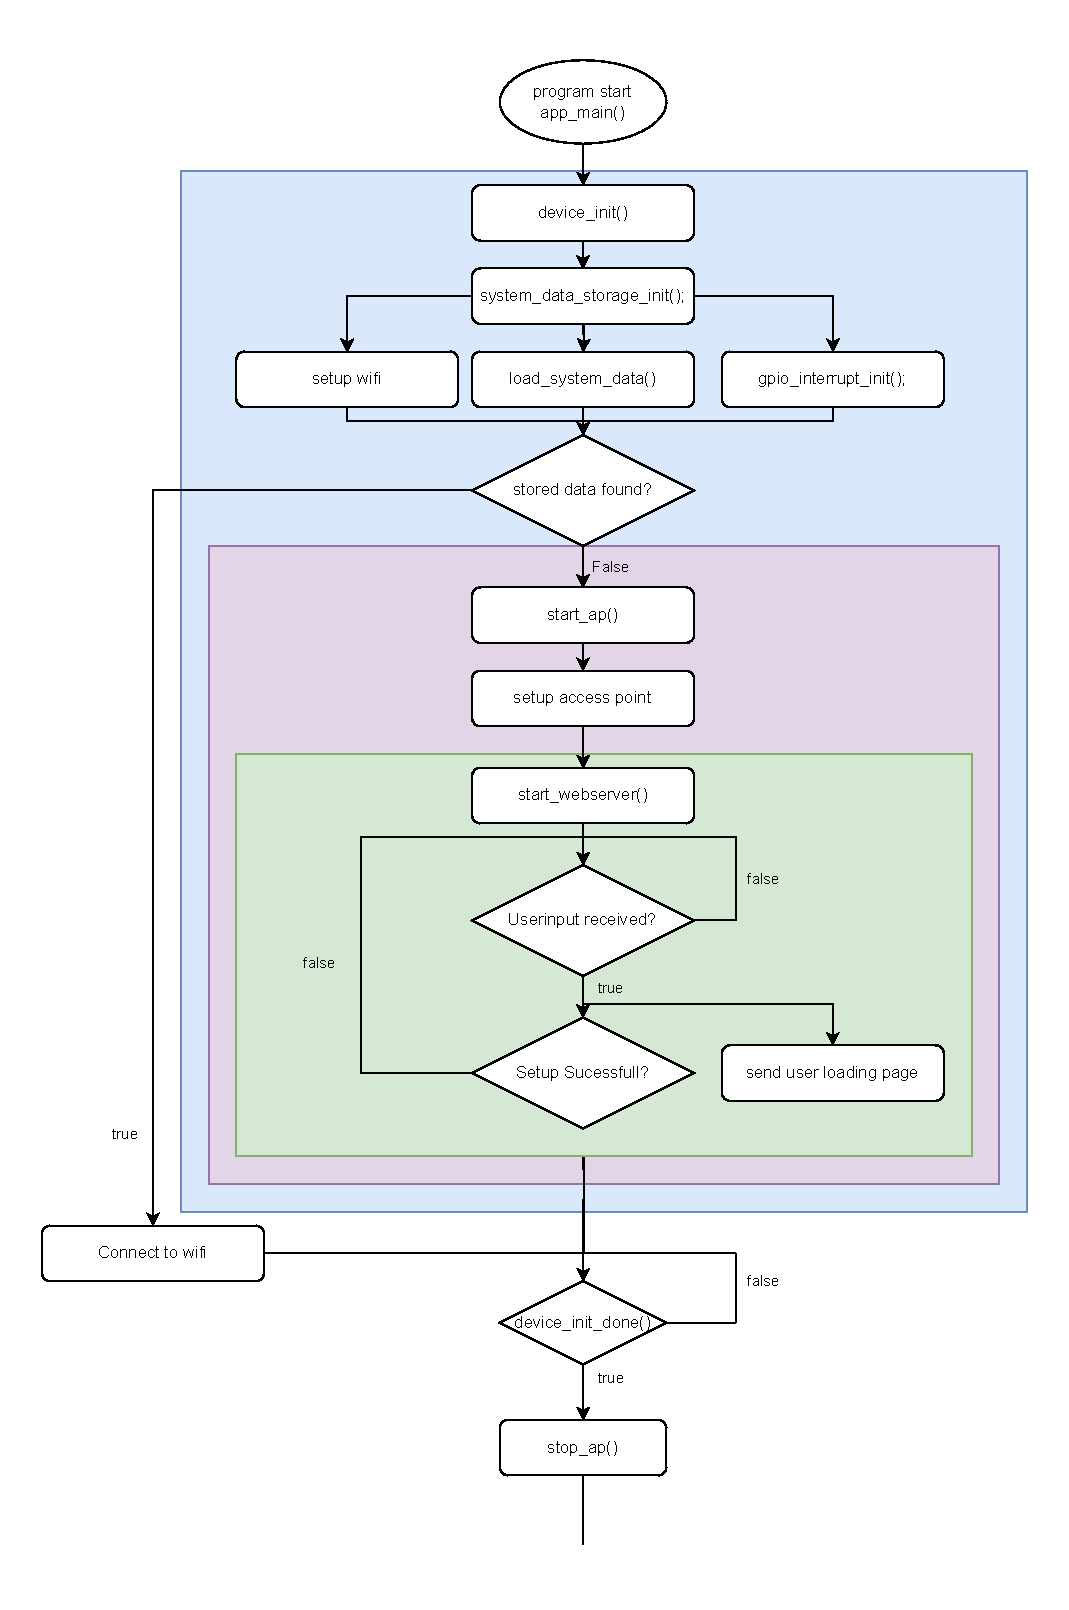
\includegraphics[width=1.1\textwidth, height=0.95\textheight, keepaspectratio]{./img/ESP_PAP.drawio.pdf}
	\caption{Ablaufplan Initialisierung des ESP}
	\label{fig:pap_esp32}
\end{figure}
\newpage

\subsubsection{Initialisierung des persistenten Speichers (NVS):}  
Der erste Schritt der Initialisierung besteht in der Aktivierung des nichtflüchtigen Speichers. Hierbei wird der sogenannte Non-Volatile Storage (NVS) über die Funktion \texttt{\url{nvs\_flash\_init()}} initialisiert. Dieser dient als zentrale, dauerhaft verfügbare Speicherstruktur zur Ablage von Konfigurationsdaten wie WLAN-Zugang, Authentifizierungstoken oder Zielwerten der Sensorik. Sollte der Speicher beschädigt sein oder durch ein Versionsupdate inkonsistent geworden sein, wird dies über die Rückgabecodes
\\
\texttt{ESP\_ERR\_NVS\_NO\_FREE\_PAGES} oder \texttt{ESP\_ERR\_NVS\_NEW\_VERSION\_FOUND} erkannt. 
\\
In diesem Fall wird über \texttt{nvs\_flash\_erase()} ein vollständiger Reset des Speichers durchgeführt. Die Architektur ist damit gegen veraltete oder inkonsistente Daten abgesichert und stellt eine fehlerfreie Persistenzlogik sicher.

\subsubsection{Laden und Strukturierung der Systemdaten:}  
Nach erfolgreicher NVS-Initialisierung wird über \texttt{load\_system\_data()} versucht, die Konfigurationsstruktur \texttt{system\_data\_t} aus dem Speicher zu laden. Diese Struktur enthält die meisten betriebskritischen Parameter, darunter:
\begin{itemize}
	\item Sensora-Nutzername,
	\item MQTT-Zugangsdaten (Benutzername, Passwort, Topics),
	\item Controller-Identifikation (ID, Modell),
	\item Sensor-Zielwerte (z.\,B. Bodenfeuchte, Temperatur, Luftfeuchte, Licht),
	\item Token für die Authentifizierung (Hardware und Software),
	\item Registrierungsstatus.
\end{itemize}
Ist der Speicherzugriff erfolgreich und die Daten konsistent, werden sie in einer lokalen Instanz gespeichert und stehenso für weitere verwendung zur Verfügung. Andernfalls verbleibt das System im Zustand \enquote{unregistriert} und leitet automatisch in den Setup-Modus über. 
\\
Zusätlich wird versucht die WLAN-Daten aus dem NVS zu laden. Diese sind werden allerdings direkt vom \texttt{esp\_wifi} Modul verwaltet und sind daher nicht Bestandteil der \texttt{system\_data\_t}-Struktur. Die WLAN-Daten werden über die Funktion \texttt{esp\_wifi\_get\_config()} geladen und in einer lokalen Instanz gespeichert. Diese Daten sind für die Registrierung des Geräts am Backend erforderlich und werden im weiteren Verlauf benötigt. Sind sie nicht vorhanden so wird das System ebenfalls in den Setup-Modus versetzt.

\subsubsection{Initialisierung der Status-LED:}  
Die Status-LED dient als primäres Feedbackinstrument für den Benutzer. Die LED ist über GPIO 2 angebunden und wird über das Modul \texttt{led\_control.c} gesteuert. Nach \texttt{led\_init()} ist der Pin als Ausgang initialisiert und standardmäßig deaktiviert. Die Logik unterscheidet mehrere Zustände:
\begin{itemize}
	\item \texttt{led\_blink\_start()}: SoftAP-Modus aktiv,
	\item \texttt{led\_on()}: System betriebsbereit und registriert,
	\item \texttt{led\_off()}: Fehlerzustand oder Resetphase.
\end{itemize}
Die Blinklogik ist als separate FreeRTOS-Task realisiert und damit unabhängig vom Hauptprogrammzyklus ausführbar, was insbesondere für Interrupt-gesteuerte Prozesse wie den Reset-Button entscheidend ist.
\\
Die aufruf der \texttt{led\_init()} erfolgt direkt nach der NVS-Initialisierung innerhalb der \texttt{device\_init()}. Dies stellt sicher, dass die LED-Logik auch bei einem Reset des NVS sofort verfügbar ist. 
\subsubsection{Einrichtung des Hardware-Resets via GPIO:}  
Um einen vollständigen Werksreset zu ermöglichen, wurde GPIO 0 als Eingangsquelle mit Pull-Up-Widerstand und fallender Flanke konfiguriert. Wird der Taster gedrückt, löst die Interrupt-Service-Routine \texttt{gpio\_isr\_handler()} eine Notification aus, die an die Task \texttt{reset\_task()} übergeben wird. Diese prüft, ob der Taster mindestens fünf Sekunden lang gedrückt bleibt. Während der Haltezeit blinkt die LED, um visuelles Feedback zu geben. Wird die Haltezeit überschritten, erfolgt:
\begin{enumerate}
	\item Stoppen des Wi-Fi-Treibers,
	\item Zurücksetzen der WLAN-Konfiguration (\texttt{esp\_wifi\_restore()}),
	\item Löschen aller Systemdaten aus dem NVS (\texttt{erase\_system\_data()}),
	\item Neustart des Controllers (\texttt{esp\_restart()}).
\end{enumerate}
Diese robuste, mehrstufige Logik verhindert unbeabsichtigte Rücksetzungen und garantiert eine sichere Wiederherstellung des Auslieferungszustands.

\subsubsection{Netzwerkstack und Eventsystem:}  
Die nächsten Initialisierungsschritte betreffen die Netzwerkkommunikation. Über \texttt{\url{esp\_netif\_init()}} wird die TCP/IP-Stack-Grundstruktur geladen. Anschließend wird ein zentraler Event-Loop mit \texttt{esp\_event\_loop\_create\_default()} erstellt, der später für alle netzwerkbezogenen Ereignisse zuständig ist. Zwei Interfaces werden parallel konfiguriert:
\begin{itemize}
	\item \texttt{esp\_netif\_create\_default\_wifi\_sta()} für den Station-Modus,
	\item \texttt{esp\_netif\_create\_default\_wifi\_ap()} für den SoftAP-Modus.
\end{itemize}
Durch die parallele Konfiguration kann der Controller sowohl als Client im Heimnetzwerk als auch als Access Point zur Erstkonfiguration agieren.

\subsubsection{Wi-Fi-Initialisierung und Event-Handler:}  
Das Wi-Fi-Modul wird über \texttt{esp\_wifi\_init()} mit einer Default-Konfiguration aktiviert. Die Registrierung von Event-Handlern erfolgt für zwei Eventtypen:
\begin{itemize}
	\item \texttt{WIFI\_EVENT}: Reaktion auf Verbindungsstart, -abbruch und Authentifizierungsfehler.
	\item \texttt{IP\_EVENT\_STA\_GOT\_IP}: Signalisiert erfolgreiche IP-Vergabe im Station-Modus.
\end{itemize}
Sobald eine Verbindung hergestellt ist und eine IP-Adresse bezogen wurde, wird der Status in der LED reflektiert. Bei mehrfachen Verbindungsabbrüchen (>5) wird automatisch in den AP-Modus zurückgeschaltet, um einen Konfigurationsfehler beheben zu können.

\subsubsection{Entscheidung über den Betriebsmodus (STA vs. SoftAP):}  
Die Entscheidung, ob das Gerät im Betriebsmodus (WLAN-Client) oder Setup-Modus (Access Point) starten soll, basiert auf den geladenen Systemdaten. Sind sowohl WLAN-Zugangsdaten als auch ein positiver Registrierungsstatus im NVS gespeichert, erfolgt der Start im STA-Modus. Der Controller versucht über \texttt{esp\_wifi\_set\_mode(WIFI\_MODE\_STA)} und \texttt{esp\_wifi\_start()} eine Verbindung aufzubauen. Andernfalls startet das System im SoftAP-Modus über \texttt{start\_ap()}.

\subsubsection{SoftAP-Modus und Webserver zur Konfiguration:}  
Im Setup-Modus stellt das System einen offenen WLAN-Access-Point mit dem Namen \enquote{Sensora} bereit. Parallel dazu wird ein HTTP-Webserver gestartet, der ein in \texttt{\url{wifi\_setup\_html.h}} eingebettetes Formular zur Verfügung stellt. Hier können SSID, Passwort und Benutzername eingegeben werden. Nach der Formulareinsendung wird über \texttt{esp\_wifi\_set\_config()} die neue Konfiguration übernommen und ein Verbindungsversuch gestartet. Eine JavaScript-basierte Statusabfrage im Browser informiert über Fortschritt und Fehlerzustände (z.\,B. keine Verbindung oder Backend nicht erreichbar). Die Benutzereingaben werden in der Systemstruktur gespeichert und sind ab diesem Moment Bestandteil der persistierten Konfiguration.

\subsubsection{Geräteregistrierung über den Authentifizierungsdienst:}  
Nach erfolgreichem Verbindungsaufbau über die im Webinterface eingegebenen WLAN-Daten wird die Registrierung des Geräts ausgelöst. Diese erfolgt über die Funktion \texttt{\url{register\_device()}} im Modul \texttt{auth\_service.c}. Ziel des Prozesses ist es, den Controller eindeutig beim zentralen Authentifizierungsserver zu identifizieren und verschlüsselte Zugangsdaten für den MQTT-Broker zu erhalten. Die Logik basiert auf einem mehrstufigen Challenge-Response-Verfahren mit HMAC-gesicherter Kommunikation und symmetrischer Fernet-Verschlüsselung (basierend auf AES-128 im CBC-Modus).

Die Registrierung umfasst folgende Schritte:
\begin{enumerate}
	\item Erstellung eines HMAC-basierten Token-Hashes aus Hardware- und Software-Token.
	\item Senden des Hashes zusammen mit dem Benutzernamen an die API \texttt{\url{/api/controller/init}}.
	\item Empfang einer zufälligen Challenge vom Server (Base64-codiert).
	\item Berechnung einer HMAC-Response auf Basis der Challenge und des Hardware-Tokens.
	\item Antwort über die API \texttt{/api/controller/verify}, zusammen mit dem ursprünglichen Token-Hash.
	\item Erhalt eines Fernet-codierten Credential-Tokens, das folgende Informationen enthält:
	\begin{itemize}
		\item MQTT-Benutzername und Passwort,
		\item Controller-ID und Modell,
		\item Publish- und Subscribe-Topics,
		\item Broker-URL, Port und SSL-Informationen.
	\end{itemize}
\end{enumerate}

\noindent Zur Validierung der Authentizität des Tokens sendet der Server zusätzlich einen sogenannten \texttt{credential\_key}, der lokal gegen einen HMAC-Vergleichswert verifiziert wird. Erst wenn diese Validierung erfolgreich ist, beginnt die Entschlüsselung des Tokens.

\subsubsection{Manuelle Implementierung der Fernet-Entschlüsselung:}  
Da im ESP32/ESP-IDF-Ökosystem keine native Unterstützung für Fernet besteht, wurde die gesamte Entschlüsselungslogik auf Byte-Ebene manuell umgesetzt. Diese umfasst:
\begin{itemize}
	\item Umwandlung von URL-safe Base64 in reguläres Base64 (inkl. Padding-Korrektur),
	\item Decodierung des Tokens mit \texttt{mbedtls\_base64\_decode()},
	\item Extraktion von Version, Timestamp, IV, Ciphertext und HMAC aus dem dekodierten Token,
	\item HMAC-Validierung des Tokens mit dem empfangenen Schlüssel zur Integritätsprüfung,
	\item Entschlüsselung des Payloads mit AES-128 im CBC-Modus über \texttt{\url{mbedtls\_aes\_crypt\_cbc()}},
	\item Entfernung und Validierung des PKCS\#7-Paddings.
\end{itemize}

Diese Implementierung stellte hohe Anforderungen an Genauigkeit im Umgang mit Speicherpuffern, Byte-Reihenfolgen und Formatierungsvorgaben. Zur Validierung wurden sämtliche Zwischenstände gegen Python-Referenzwerte getestet. Fehler in Padding-Handling oder IV-Länge führten während der Entwicklung regelmäßig zu Speicherverletzungen oder inkorrekten Dekodierungen. Dadurch wurde die Notwendigkeit einer präzisen und robusten Implementierung deutlich. Die gesamte Logik ist in der Funktion \texttt{decrypt\_fernet\_token()} im Modul \texttt{auth\_service.c} zusammengefasst.

\subsubsection{Speicherung und Abschluss der Registrierung:}  
Nach erfolgreicher Entschlüsselung werden alle empfangenen Felder aus dem Credential-Payload in die Struktur \texttt{system\_data\_t} überführt. Zusätzlich wird der Registrierungsstatus auf \texttt{true} gesetzt. Der gesamte Datenblock wird abschließend über \texttt{save\_system\_data()} dauerhaft im Flash gespeichert. Temporäre Speicherbereiche für MQTT-Daten und URLs werden aus dem Heap freigegeben. Dieser Mechanismus sichert sowohl Speicherstabilität als auch Datenintegrität und bildet die Basis für alle folgenden Kommunikationsprozesse.

\subsubsection{Abschluss der Initialisierung durch Deaktivierung des Setup-Modus:}  
Sobald Registrierung und Netzwerkverbindung erfolgreich abgeschlossen sind, endet eine while Schleife in \texttt{app\_main()}, da die Funktion \texttt{device\_init\_done} nun true returned. Danach wird der Setup-Modus beendet. Hierzu erfolgt im Hauptprogramm \texttt{app\_main()} ein expliziter Aufruf von \texttt{stop\_ap()}. Diese Funktion schaltet den Access Point ab, stoppt den HTTP-Webserver und wechselt den Betriebsmodus von \texttt{WIFI\_MODE\_APSTA} nach \texttt{WIFI\_MODE\_STA}. Dabei wird sichergestellt, dass keine Verbindungsversuche mehr mit dem offenen Netzwerk erfolgen und alle Schnittstellen auf eine abgesicherte Betriebsumgebung migriert werden.
\\
Ein typischer Ablauf von \texttt{stop\_ap()} umfasst:
\begin{enumerate}
	\item Überprüfung des aktuellen Betriebsmodus,
	\item Abschaltung des Webservers mit \texttt{httpd\_stop()},
	\item Wechsel in den reinen STA-Modus mittels \texttt{esp\_wifi\_set\_mode()},
	\item Soft-Restart des Wi-Fi-Treibers zur Sicherstellung eines sauberen Zustands,
	\item Reconnect-Versuch zur bekannten SSID bei verlorener Verbindung (optional),
	\item LED-Signalisierung durch Stoppen des Blinkens und dauerhaftes Einschalten.
\end{enumerate}

\noindent Diese Umstellung ist notwendig, da der SoftAP-Modus als temporäres Konfigurationsmittel konzipiert ist und im Normalbetrieb ein Sicherheitsrisiko darstellen würde.

\subsubsection{Abschlussprüfung der Initialisierung:}  
Nach Durchführung aller Schritte verbleibt das System im verbundenen, registrierten Zustand und ist bereit zur Ausführung der nachgelagerten Subsysteme. Der Status wird über die Funktion \texttt{device\_init\_done()} regelmäßig geprüft. Diese liefert den Wert \texttt{true}, sobald sowohl eine gültige IP-Adresse bezogen wurde (\texttt{is\_sta\_connected()}) als auch der \texttt{registered}-Status in \texttt{system\_data\_t} auf \texttt{true} gesetzt ist.

Erst wenn diese Bedingung erfüllt ist, werden in \texttt{app\_main()} die weiteren Initialisierungen durchgeführt:
\begin{itemize}
	\item Zeitsynchronisation mit SNTP über \texttt{initialize\_sntp()} und \texttt{wait\_for\_time\_sync()},
	\item Initialisierung der MQTT-Verbindung über \texttt{solace\_init()},
	\item Start der Sensorik und Bewässerungslogik.
\end{itemize}

\noindent Der Initialisierungsprozess ist damit abgeschlossen. Das System befindet sich fortan im überwachten Betriebsmodus und kann vollständig autonom auf externe Kon

    \subsection{Regelbetrieb des ESP}

Zentral bei der Umsetzung des automatisierten Bewässerungssystems ist der ESP32-WROOM-32D Mikrocontroller, welcher die Interaktion zwischen Sensorik, Aktorik und Backend-Systemen steuert. Dabei stellt dieser ESP32 eine umfangreichen GPIO-Ausstattung, welche den Anschluss verschiedenster Peripheriekomponenten ermöglicht.
\\
Im Anschluss an die ESP-Initialisierung, die mittels Wifi-Provisioning sowie Authentifizierung gegen den Backend-Service die Konnektivität sicherstellt, beginnt der zyklische Programmablauf, welcher in verschiedene, klar voneinander getrennte Komponenten untergliedert ist. Diese sind modular aufgebaut und folgen einem Event-Loop-Modell, wie es in Echtzeitbetriebssystemen (RTOS) wie FreeRTOS üblich ist. Die zentrale Steuerung erfolgt durch Tasks, welche Sensorwerte erfassen, verarbeiten, und basierend darauf Aktionen wie etwa die Aktivierung der Pumpe auslösen.
\\
Zur Erfassung der Umweltbedingungen kommen drei Sensoren zum Einsatz: ein \textit{GY-302 BH1750} zur Messung der Beleuchtungsstärke, ein \textit{DHT11}-Sensor zur Ermittlung von Temperatur und Luftfeuchtigkeit sowie ein kapazitiver Bodenfeuchtigkeitssensor (\textit{HiLetgo LM393}). Die Ausgabe der gesammelten Sensordaten erfolgt in periodischen Intervallen über MQTT an eine Solace PubSub Instanz, die über ein Docker-Container-System bereitgestellt wird.
\\
Im Folgenden wird jeder Abschnitt des abstrahierten Ablaufplans des ESP-Regelbetriebs, zu sehen in Abbildung \vref{fig:esp_regelbetrieb}, technisch und funktional erläutert.


\begin{figure}[H]
	\centering
	\vspace{0pt} % verhindert Abstand oben
	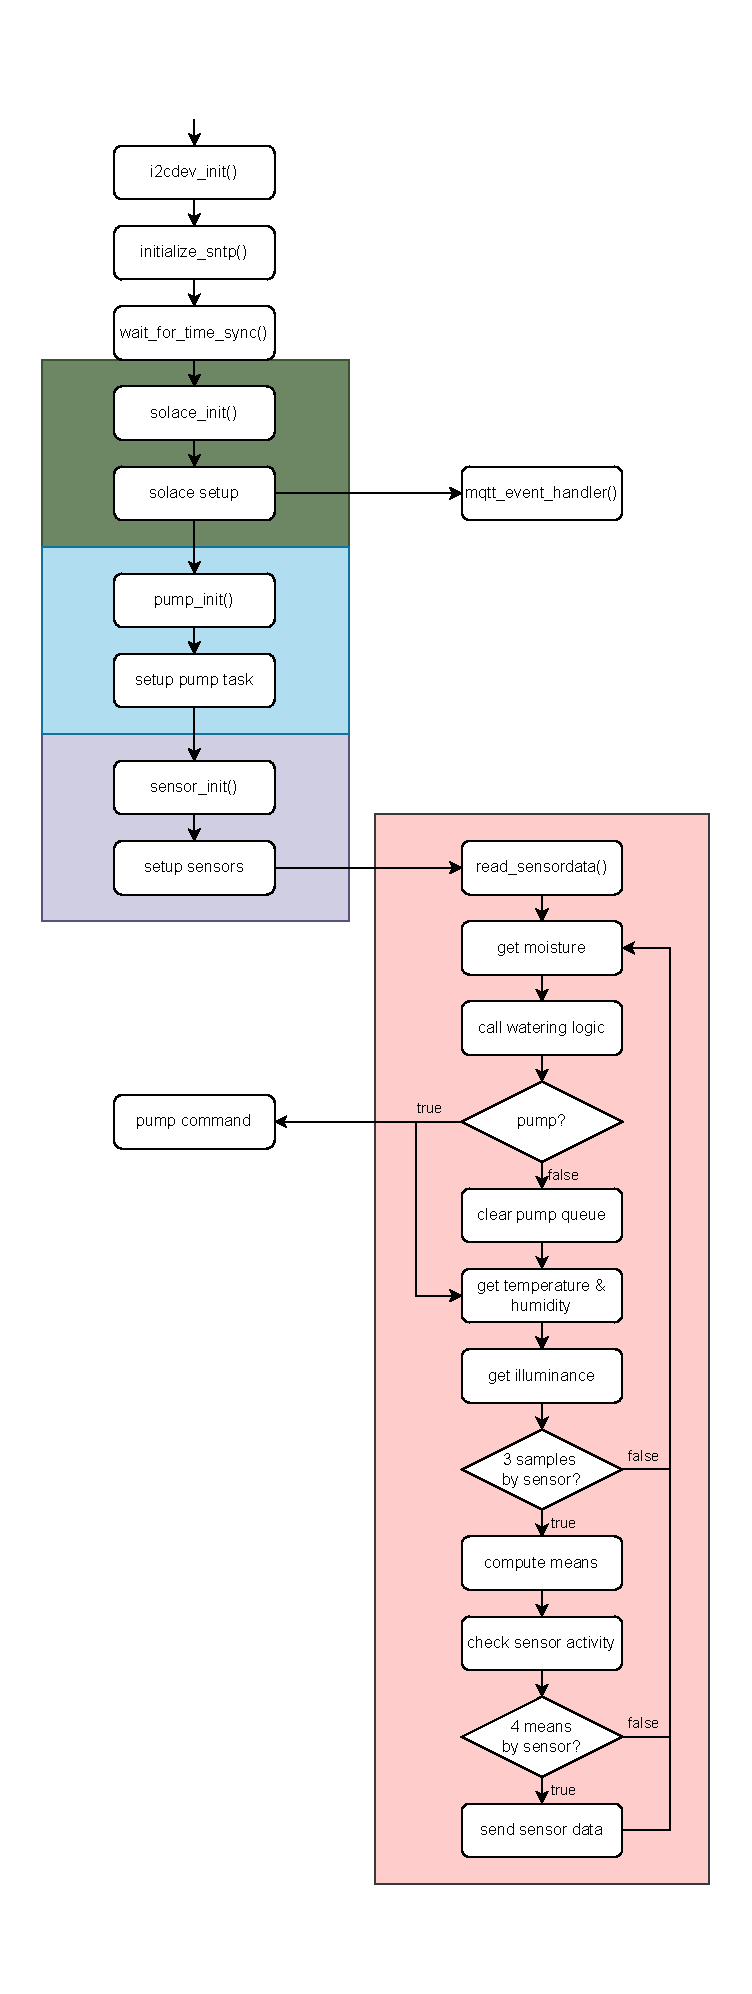
\includegraphics[height=0.97\textheight, keepaspectratio]{./img/esp_regelbetrieb.pdf}
	\caption{Ablaufplan Regelbetrieb des ESP}
	\label{fig:esp_regelbetrieb}
\end{figure}
\newpage

\subsubsection{Systemvorbereitungen: I\textsuperscript{2}C-Stack und Zeitdienst}

Nach Beendigung der initialen Gerätekonfiguration und Abschaltung des Access Points (\texttt{stop\_ap()}) beginnt der ESP32 im Regelbetrieb mit einer Reihe vorbereitender Initialisierungen, die für die korrekte Funktion der Sensorik und Kommunikation essenziell sind. Im Ablaufplan (Abbildung \vref{fig:esp_regelbetrieb}) ist dieser Schritt durch die folgenden Funktionsaufrufe dargestellt:

\begin{itemize}
	\item \texttt{i2cdev\_init()}
	\item \texttt{initialize\_sntp()}
	\item \texttt{wait\_for\_time\_sync()}
\end{itemize}
\vspace{1em}

\noindent Die erste vorbereitende Maßnahme ist die Initialisierung des I\textsuperscript{2}C-Stacks. Die Funktion \texttt{i2cdev\_init()} stammt aus einer externen Bibliothek und abstrahiert die Konfiguration des I\textsuperscript{2}C-Busses, welcher für die Kommunikation mit dem BH1750-Lichtsensor erforderlich ist. Der Sensor wird über die standardisierte I\textsuperscript{2}C-Schnittstelle betrieben und benötigt einen initialisierten Treiberstack, bevor Lese- oder Schreibzugriffe erfolgen können. Im Falle eines Fehlers bei der Initialisierung wird der Systemstart abgebrochen und eine entsprechende Fehlermeldung ausgegeben. Diese Maßnahme dient der Robustheit und stellt sicher, dass keine fehlerhaften Sensordaten erzeugt werden, die zu falschen Bewässerungsentscheidungen führen könnten.
\\
Im Anschluss an die I\textsuperscript{2}C-Vorbereitung erfolgt die Synchronisierung der Systemzeit über das Simple Network Time Protocol (SNTP). Die korrekte Zeit ist essenziell, da alle Sensordaten, die später an das Backend übertragen werden, mit Zeitstempeln versehen werden. Diese Zeitstempel sind wiederum entscheidend für die korrekte Interpretation und Verarbeitung im Backend, insbesondere in Systemen, die auf Zeitreihenanalysen oder historischen Vergleichswerten basieren.
\\
Die Funktion \texttt{initialize\_sntp()} konfiguriert einen SNTP-Client im Polling-Modus und setzt den verwendeten Zeitserver (standardmäßig \texttt{pool.ntp.org}). Anschließend wird in der Funktion \texttt{wait\_for\_time\_sync()} geprüft, ob eine gültige Systemzeit empfangen wurde. Diese Überprüfung erfolgt durch wiederholtes Abfragen der lokalen Zeitinformationen. Der Ablauf ist so gestaltet, dass der ESP32 so lange blockiert, bis eine Zeit verfügbar ist, deren Jahr größer als 2016 ist – dies dient als Heuristik für eine erfolgreiche Synchronisierung.
\\
Diese Zeitsynchronisation ist ein zentrales Qualitätsmerkmal des Systems, da sie nicht nur zur Zeitstempelung der Messwerte dient, sondern auch für die Vergleichbarkeit mit Zielwerten im Backend sowie für langfristige Protokollierungen notwendig ist. Eine falsch synchronisierte Uhr würde beispielsweise zu verzerrten Zeitreihen führen und könnte fehlerhafte Rückschlüsse auf das Verhalten der Pflanzen oder das Klimaregime erlauben.
\\
Insgesamt dienen die beschriebenen Systemvorbereitungen also sowohl der Sicherstellung einer funktionierenden Peripheriekommunikation (über I\textsuperscript{2}C) als auch der korrekten zeitlichen Einordnung aller Mess- und Steuerdaten (über SNTP). Beide Schritte bilden somit eine essenzielle Grundlage für den nachfolgenden zyklischen Ablauf im Regelbetrieb.

\subsubsection{MQTT-Kommunikationsclient}

Nach Abschluss der systemnahen Initialisierungen folgt im Regelbetrieb die Anbindung an die Backend-Infrastruktur über das MQTT-Protokoll. Dies erfolgt durch den Aufruf der Funktion \texttt{solace\_init()}, welche im Ablaufplan (Abbildung \vref{fig:esp_regelbetrieb}) das \enquote{solace setup} sowie den \texttt{mqtt\_event\_handler()} anstößt.
\\
Die MQTT-Kommunikation basiert in diesem System auf dem Publish-Subscribe-Modell und erfolgt über eine Solace PubSub Instanz, welche als Docker-Container bereitgestellt wird. Der ESP32 agiert dabei als Publisher und Subscriber zugleich: Er veröffentlicht periodisch aggregierte Sensordaten und empfängt gleichzeitig neue Zielwerte zur Parametrisierung der Regelstrategie (z.\,B. Soll-Bodenfeuchtigkeitswerte).
\\
Im Rahmen der \texttt{solace\_init()}-Funktion werden zunächst die aus dem nichtflüchtigen Speicher geladenen Verbindungsparameter wie Benutzername, Passwort, Client-ID sowie die spezifischen Topics konfiguriert. Anschließend wird der MQTT-Client initialisiert und mit dem Broker verbunden. Die Verbindung wird dabei so konfiguriert, dass keine Session-Daten zurückgesetzt werden (\texttt{disable\_clean\_session = true}), was eine persistente Kommunikationsbeziehung zwischen Controller und Broker ermöglicht.
\\
Nach erfolgreicher Verbindung registriert der Client einen Event-Handler, der unter anderem auf das Eintreffen neuer Datenpakete reagiert. Ein zentrales Element dieser Kommunikation ist die Funktion \texttt{send\_message()} (zu sehen unter Listing \vref{lst:send_data}), welche zum Versand der aggregierten Sensordaten dient. Diese Funktion nimmt eine bereits als JSON-formatierte Zeichenkette entgegen und überträgt diese mithilfe des MQTT-Clients auf das konfigurierte Topic:
\\

\begin{lstlisting}[style=cstyle, caption={Senden der Sensordaten}, label={lst:send_data}]
	void send_message(const char *message) {
		if (message != NULL) {
			esp_mqtt_client_enqueue(client, info.solace_publish_topic, message, 0, 1, 1, true);
		}
	}
\end{lstlisting}
\vspace{1em}
\noindent Die Nutzung der Funktion \texttt{esp\_mqtt\_client\_enqueue()} ermöglicht dabei eine nicht-blockierende Übertragung, bei der die Nachricht in die interne Queue des MQTT-Stacks geschrieben wird. Durch das Setzen der QoS-Stufe (Quality of Service) auf 1 wird sichergestellt, dass die Nachricht mindestens einmal zuverlässig zugestellt wird – ein angemessener Kompromiss zwischen Zuverlässigkeit und Latenz für diese Anwendungsklasse.
\\
Umgekehrt werden eingehende Steuerinformationen, die z.\,B. neue Zielwerte für Bodenfeuchte, Temperatur oder Beleuchtung enthalten, vom Event-Handler verarbeitet, sobald eine MQTT-Nachricht auf dem Subscription-Topic eintrifft. In diesem Fall wird der Nachrichtenspeicher zunächst allokiert und die empfangenen Daten sicher aus dem Event-Buffer kopiert, wie in folgendem Listing \vref{lst:receive_data} zu sehen ist:
\\

\begin{lstlisting}[style=cstyle, caption={Empfangen von Solace-Daten}, label={lst:receive_data}]
	char *msg = malloc(event->data_len + 1);
	if (msg == NULL) {
		break;
	}
	memcpy(msg, event->data, event->data_len);
	msg[event->data_len] = '\0';
	
	process_received_json(msg);
	
	free(msg);
\end{lstlisting}
\vspace{1em}
\noindent Die manuelle Speicherverwaltung (Allokation und Freigabe) stellt sicher, dass keine Datenverluste auftreten, wenn mehrere MQTT-Ereignisse in schneller Folge eintreffen. Der Zwischenschritt über \texttt{memcpy()} ist notwendig, da der Zeiger \texttt{event->data} nur innerhalb des Event-Kontexts gültig ist. Nach dem Kopieren wird der Inhalt an die Funktion \texttt{process\_received\_json()} übergeben, welche das JSON-Objekt parst und die enthaltenen Zielwerte in den persistenten Flash-Speicher schreibt. Dadurch werden Sollwerte zur Laufzeit aktualisiert und unmittelbar im weiteren Sensorzyklus wirksam.
\\
Insgesamt übernimmt die MQTT-Client-Initialisierung eine zentrale Rolle im System, da sie die bidirektionale Kommunikation zwischen Hardware-Controller und Backend sicherstellt. Sie erlaubt nicht nur die kontinuierliche Datenerfassung und -übermittlung, sondern auch die Fernparametrierung des Systems durch das Backend. Das asynchrone Design mit Event-Handlern, QoS-gestütztem Datentransport und stabiler Speicherverwaltung entspricht den Anforderungen moderner IoT-Anwendungen hinsichtlich Robustheit, Modularität und Echtzeitfähigkeit. \\
Desweiteren wird der verwendete MQTT-Client mit einem automatischen Reconnect-Mechanismus betrieben, um eine hohe Verfügbarkeit der Kommunikation sicherzustellen. Tritt ein Verbindungsabbruch auf, erkennt der zugrunde liegende MQTT-Client der ESP-IDF diesen Fall und übernimmt selbstständig Wiederverbindungsversuche. Dieses Verhalten ist in Echtzeitsystemen mit instabiler oder intermittierender Netzwerkverbindung besonders vorteilhaft, da es die Notwendigkeit eines externen Fehlerbehandlungsmechanismus minimiert und die Robustheit des Systems erhöht. Ein manueller Eingriff durch das Backend ist in solchen Fällen nicht erforderlich.

\subsubsection{Initialisierung der Aktorik (Pumpe)}

Die Initialisierung der Pumpensteuerung erfolgt über die Funktion \texttt{pump\_init()}, welche zwei grundlegende Aufgaben erfüllt: Einerseits wird der für die Relaisansteuerung vorgesehene GPIO-Pin hardwareseitig konfiguriert und initial in einen definierten Zustand versetzt (High = Relais aus), andererseits wird eine dedizierte FreeRTOS-Task mit dem Namen \texttt{pump\_task} gestartet, die in der Abbildung \vref{fig:esp_regelbetrieb} unter \enquote{setup pump task} zu erkennen ist. Diese Task ist dauerhaft aktiv und wartet blockierend auf neue Steuerbefehle, welche durch die Sensorik generiert werden.
\\
Die Pumpe selbst wird über ein SRD-05VDC-SL-C Relaismodul gesteuert, das bei Aktivierung den Stromkreis zur Wasserpumpe schließt. Die Softwarelogik verwendet dazu die \texttt{gpio\_set\_level()}-Funktion, um den Relaiskontakt aktiv (Low) oder inaktiv (High) zu schalten. Eine Initialisierung mit eindeutigem Anfangszustand ist dabei essenziell, um ungewolltes Aktivieren der Pumpe beim Systemstart zu verhindern.
\\
Die Task \texttt{pump\_task} wird über die FreeRTOS-Funktion \texttt{xTaskCreatePinnedToCore()} auf Core 1 des ESP32 platziert. Diese Kernzuweisung erfolgt bewusst, um eine Lastverteilung zwischen Kommunikations- und Sensor-/Aktorlogik zu ermöglichen. Da der WLAN-Stack sowie der MQTT-Client auf Core 0 des ESP32 betrieben werden, ergibt sich durch diese Trennung eine höhere Echtzeitfähigkeit der Pumpenlogik und eine geringere Interferenz zwischen den Tasks. Diese Architekturentscheidung trägt zur Stabilität und deterministischen Ausführung der Aktorik bei, insbesondere unter hoher Netzwerklast. 
\\
Die in Listing \vref{lst:pump_task} gezeigte Erstellung der \texttt{pump\_task} wurde mit einer Priorität von \texttt{5} gewählt, da sie auf eingehende Steuerbefehle schnell und zuverlässig reagieren muss. Die höhere Priorität stellt sicher, dass Pumpvorgänge bevorzugt behandelt werden. Die Stackgröße von \texttt{2048 Bytes} ist ausreichend, da die Task nur einfache Befehle verarbeitet und keine speicherintensiven Operationen durchführt.
\newpage

\begin{lstlisting}[style=cstyle, caption={Start der Pump-Task}, label={lst:pump_task}]
	BaseType_t result = xTaskCreatePinnedToCore(
	pump_task,           // Task-Funktion
	"pump_task",         // Name
	2048,                // Stackgroesse
	NULL,                // Parameter
	5,                   // Prioritaet
	NULL,                // Handle (nicht verwendet)
	1                    // Core 1
	);
\end{lstlisting}
\vspace{1em}
\noindent Neben der Task-Erzeugung wird eine Queue \texttt{pumpQueue} erstellt, welche als asynchrone Kommunikationsschnittstelle zwischen Sensorik und Aktorik dient. Über diese Queue werden Befehle der Struktur \texttt{pump\_params\_t}, welche unter anderem die gewünschte Pumpdauer enthalten, an die Aktorik weitergereicht. Dieses Kommunikationsmuster entspricht dem klassischen \textit{Producer-Consumer-Modell}, bei dem die Sensorik als Ereignisquelle (Producer) fungiert und die Aktorik aufgabenbasiert reagiert (Consumer).
\\
Die Queue dient dabei nicht nur der Synchronisation, sondern ermöglicht auch eine temporäre Entkopplung der Aufgaben. Selbst bei kurzen Verzögerungen in der Ausführung der Pumpen-Task kann ein eingehender Befehl zwischengespeichert werden, was zur Entkopplung der Sensordatenverarbeitung von der physikalischen Ausführung beiträgt. Diese Architekturentscheidung verbessert sowohl die Reaktionsfähigkeit als auch die Systemrobustheit.
\\
Die beiden im Ablaufdiagramm (vgl. Abbildung \vref{fig:esp_regelbetrieb}) aufgeführten Schritte \texttt{pump\_init()} sowie \enquote{setup pump task} stellen also die Grundlage für die Aktorik im Regelbetrieb dar und ermöglichen die automatische Umsetzung von Bewässerungsentscheidungen in hardwareseitige Steuerimpulse.

\subsubsection{Start der Sensorik-Task}

Die kontinuierliche Erfassung und Verarbeitung der Umgebungsdaten bildet das funktionale Zentrum des Regelbetriebs. Dieser Prozess wird durch die FreeRTOS-Task \\
\texttt{read\_sensordata()} realisiert, welche zyklisch die Werte aller verbauten Sensoren erfasst, bewertet, aggregiert und im Anschluss sowohl lokal verarbeitet als auch über MQTT an das Backend übermittelt. Der Start dieser Task erfolgt in der Funktion \texttt{sensor\_init()} und wird explizit dem Core 1 des ESP32 zugewiesen.
\\
Wie auch bei der parallel laufenden Pump-Task, dient die gezielte Platzierung auf Core 1 dazu, Konflikte mit systemnahen Funktionen wie WLAN- und MQTT-Kommunikation zu vermeiden, welche bevorzugt auf Core 0 abgewickelt werden. Durch diese Kerntrennung wird eine deterministische und unterbrechungsarme Ausführung der zyklischen Messprozesse gewährleistet.
\\
Die Erstellung der Task erfolgt mit einer Priorität von \texttt{2} und einer Stackgröße von \texttt{8192 Bytes}. Die moderate Priorität wurde gewählt, da die Sensorik-Task zwar regelmäßig und zuverlässig ausgeführt werden muss, jedoch nicht auf unmittelbare Reaktion angewiesen ist. Eine Priorität von \texttt{2} stellt sicher, dass die Task bei ausreichenden Ressourcen regelmäßig eingeplant wird, jedoch gegenüber zeitkritischeren Prozessen – wie etwa der Pumpensteuerung mit Priorität \texttt{5} – zurücktritt. Diese Priorisierung entspricht den Anforderungen eines Echtzeitsystems, in dem Datenaufnahme zwar zeitnah, jedoch nicht unbedingt unterbrechungsfrei ablaufen muss.
\\
Die vergleichsweise große Stackgröße von \texttt{8192 Bytes} wurde gewählt, um der erhöhten Speicheranforderung durch folgende Faktoren Rechnung zu tragen:
\\
\begin{itemize}
	\item Speicherung mehrerer Sensorwerte und Mittelwerte in Arrays,
	\item Verarbeitung mehrerer \texttt{cJSON}-Objekte bei der MQTT-Nachrichtenerstellung,
	\item Nutzung zusätzlicher Hilfsfunktionen (z.\,B. Zeitstempelerzeugung, Statusprüfung),
	\item Absicherung gegen potenzielle Stacküberläufe bei komplexeren JSON-Strukturen.
\end{itemize}

\vspace{1em}

\begin{lstlisting}[style=cstyle, caption={Start der Sensorik-Task}, label={lst:sensor_task}]
	xTaskCreatePinnedToCore(
	&read_sensordata,     // Task-Funktion
	"read_sensordata",    // Name
	8192,                 // Stackgroesse in Bytes
	NULL,                 // Parameter
	2,                    // Prioritaet
	NULL,                 // Handle (nicht benoetigt)
	1                     // Core-ID
	);
\end{lstlisting}
\vspace{1em}

\noindent Im Ablaufdiagramm (vgl. Abbildung \vref{fig:esp_regelbetrieb}) ist der gesamte Funktionsblock der Sensorik-Task im unteren Bereich dargestellt, beginnend mit dem Schritt \texttt{read\_sensordata()}. Innerhalb der Task werden in einem fortlaufenden Loop nacheinander die Messwerte aller Sensoren erfasst. Dazu zählen:
\\
\begin{itemize}
	\item die Bodenfeuchte über den kapazitiven Sensor (ADC),
	\item Temperatur und Luftfeuchte über den DHT11 (digital, GPIO),
	\item sowie die Beleuchtungsstärke über den BH1750 (I\textsuperscript{2}C).
\end{itemize}
\vspace{1em}

Die dabei gewonnenen Messwerte werden zunächst in Arrays zwischengespeichert. Sobald pro Sensor drei Einzelmessungen (\texttt{SAMPLES = 3}) vorliegen, wird ein arithmetischer Mittelwert gebildet. Dies erfolgt zur Rauschunterdrückung und Glättung von Ausreißern, welche etwa durch Störimpulse oder instabile Umgebungsbedingungen entstehen können. Die entsprechende Funktion \texttt{compute\_mean()}, zu sehen unter Listing \vref{lst:mean}, summiert dazu alle Einzelwerte und berechnet daraus den Durchschnitt. Der Algorithmus ist bewusst einfach gehalten, um Rechenzeit zu sparen und eine konstante Ausführungszeit zu garantieren:
\\

\begin{lstlisting}[style=cstyle, caption={Mittelwertbildung zur Glättung von Sensorwerten}, label={lst:mean}]
	int compute_mean(const int values[]) {
		int sum = 0;
		for (int i = 0; i < SAMPLES; i++) {
			sum += values[i];
		}
		return sum / SAMPLES;
	}
\end{lstlisting}
\vspace{1em}

\noindent Vor der Weiterverarbeitung wird zusätzlich eine Validierung durchgeführt, ob der jeweilige Sensor als aktiv und funktionsfähig eingestuft werden kann. Dabei wird überprüft, ob alle Messwerte innerhalb eines gültigen Wertebereichs liegen. Dies verhindert, dass fehlerhafte Sensoren (z.\,B. durch Kabelbruch oder fehlerhafte Kalibrierung) zu ungültigen Steuerentscheidungen führen. Die Funktion \texttt{is\_sensor\_active()} übernimmt diese Plausibilitätsprüfung:
\\

\begin{lstlisting}[style=cstyle, caption={Überprüfung der Sensoraktivität}, label={lst:sensor_active}]
	bool is_sensor_active(const int values[], int sampleCount) {
		for (int i = 0; i < sampleCount; i++) {
			if (values[i] <= 0 || values[i] >= 4095) {
				return false; // Sensorfehler oder Disconnect
			}
		}
		return true;
	}
\end{lstlisting}
\vspace{1em}

\noindent Sobald vier Mittelwerte (\texttt{MEAN\_COUNT = 4}) pro Sensor vorliegen, erfolgt die Erzeugung einer strukturierten JSON-Nachricht. Diese umfasst Messwerte, Zeitstempel, Sensorstatusinformationen sowie Controller-Metadaten und wird über die zuvor erläuterte Schnittstelle \texttt{send\_message()} via MQTT an das Backend gesendet.
\\
Parallel zur Messwerterfassung wird bei jeder neuen Bodenfeuchte-Messung die Bewässerungslogik aktiviert, wie im Ablaufdiagramm unter \enquote{call watering logic} dargestellt. Die Entscheidungslogik erfolgt durch Aufruf der Funktion \texttt{calculate\_watering\_duration()}, welche im nächsten Abschnitt detailliert beschrieben wird. Führt diese Analyse zu einer positiven Bewässerungsentscheidung, wird ein entsprechender Pump-Befehl über die Funktion \texttt{pump\_send\_command()} an die globale Queue \texttt{pumpQueue} übermittelt, welche als Kommunikationsschnittstelle zur \texttt{pump\_task()} dient und die sichere, asynchrone Übergabe von Steuerbefehlen ermöglicht.
\\
Insgesamt vereint die Sensorik-Task zentrale Aufgaben der Datenerfassung, Signalverarbeitung, Qualitätssicherung, Entscheidungslogik und Backend-Kommunikation. Ihre saubere architektonische Einbindung sowie die klar definierte Schnittstelle zur Aktorik machen sie zu einem robusten und flexiblen Kernbestandteil des Gesamtsystems.

\subsubsection{Bewässerungslogik}

Die Funktion \texttt{calculate\_watering\_duration()} ist für die Ermittlung der notwendigen Bewässerungsdauer auf Basis der Differenz zwischen gemessener und Ziel-Bodenfeuchte zuständig. Sie lädt die Systemkonfiguration, vergleicht Soll- und Ist-Werte und berechnet daraus die Pumpdauer. Um Über- und Unterbewässerung zu vermeiden, wird die Dauer auf definierte Grenzwerte begrenzt.
\\
\\
Die Entscheidung darüber, ob eine Bewässerung erforderlich ist und in welchem Umfang diese erfolgen soll, wird durch die Funktion \texttt{calculate\_watering\_duration()} getroffen. Dieser Funktionsaufruf ist im Ablaufdiagramm unter dem Knoten \enquote{call watering logic} eingezeichnet und bildet das zentrale Bindeglied zwischen der gemessenen Bodenfeuchte und der Ansteuerung der Pumpenlogik.
\\
Die Funktion wird bei jeder neuen Messung der Bodenfeuchte innerhalb der Sensorik-Task aufgerufen. Sie lädt zunächst die gespeicherten Systemdaten, insbesondere den konfigurierten Zielwert für die Bodenfeuchte (\texttt{target\_moisture}) aus dem persistenten Speicher. Anschließend wird geprüft, ob der aktuelle Feuchtewert unterhalb des Sollwertes liegt. Nur wenn ein solches Defizit besteht, wird eine Pumpdauer berechnet.
\\
Wie in Listing \vref{lst:calc_duration} zu erkennen, basiert die Berechnung der Dauer auf einem linearen Modell: Die Differenz zwischen Ziel- und Istwert wird mit einem konstanten Faktor (\texttt{WATERING\_K\_FACTOR}) multipliziert, der in diesem Fall auf \texttt{100} gesetzt wird. Dieses einfache Modell erlaubt eine intuitive Parametrierung und gewährleistet eine proportionale Anpassung der Bewässerungsdauer an das Ausmaß der Trockenheit.
\newpage

\begin{lstlisting}[style=cstyle, caption={Berechnung der Bewässerungsdauer}, label={lst:calc_duration}]
	int calculate_watering_duration(int current_moisture) {
		load_system_data(&info);
		
		if (!info.target_moisture) {
			info.target_moisture = 0;
		}
		
		if (current_moisture >= info.target_moisture) {
			return 0;
		}
		
		int deficit = info.target_moisture - current_moisture;
		int duration = deficit * WATERING_K_FACTOR;
		
		if (duration < MIN_WATERING_TIME) return 0;
		if (duration > MAX_WATERING_TIME) duration = MAX_WATERING_TIME;
		
		return duration;
	}
\end{lstlisting}
\vspace{1em}

\noindent Führt die Funktion zu einer Nicht-Null-Dauer, wird das Ergebnis in Form eines \\\texttt{pump\_params\_t}-Strukturobjekts an die zuvor initialisierte Queue \texttt{pumpQueue} übergeben. Die Übergabe erfolgt über die Funktion \texttt{pump\_send\_command()}, wodurch die asynchron laufende Pumpen-Task (vgl. Listing \vref{lst:pump_task}) aktiviert wird. Dieses Systemdesign gewährleistet eine klare Trennung zwischen Entscheidung und Ausführung, was die Modularität, Wartbarkeit und Reaktionssicherheit des Systems erhöht.
\\
Zusammenfassend bildet die Funktion \texttt{calculate\_watering\_duration()} die Kernkomponente der Regelstrategie. Durch die Kombination aus Zielwertvergleich, linearer Berechnung und Schutzgrenzen wird ein praxisnahes Steuerverhalten realisiert, das zugleich einfach und robust in der Anwendung ist. Ihre Position innerhalb der Sensorik-Task erlaubt eine kontinuierliche Reaktion auf veränderte Umweltbedingungen und macht die Bewässerungsentscheidung zu einem integralen Bestandteil des zyklischen Regelbetriebs.

\subsubsection{Testen der Funktionalitäten}

Die Validierung der im Rahmen dieser Arbeit implementierten Systemfunktionen erfolgte durch eine Kombination aus lokalen Integrationstests und laufzeitbasiertem Debugging über den seriellen Monitor. Ziel war es, sowohl die Korrektheit der Sensorerfassung und Datenverarbeitung als auch die Robustheit der Kommunikations- und Aktorik-Komponenten unter realitätsnahen Bedingungen zu überprüfen.
\\
Ein zentrales Element der Testinfrastruktur war die Verwendung einer containerisierten MQTT-Broker-Umgebung auf Basis von Solace. Der Broker wurde über eine \\\texttt{docker-compose.yml}-Datei lokal bereitgestellt, welche alle relevanten Ports (u.\,a. 1883 für MQTT sowie 8080 für das Web-UI) freigibt und essenzielle Umgebungsparameter für die Broker-Verwaltung definiert. Durch diese Virtualisierung konnte eine vollständig kontrollierte und jederzeit rekonstruierbare Testumgebung geschaffen werden, ohne auf externe Dienste angewiesen zu sein.
\\
Die \texttt{docker-compose.yml} ermöglichte somit die schnelle Inbetriebnahme und erlaubte über das Web-Interface auch die manuelle Kontrolle von Topic-Inhalten, Subskriptionen sowie eingehenden Sensorwerten. Darüber hinaus konnte die Reaktion des Systems auf eingehende Steuerbefehle (z.\,B. Zielwertänderungen) in Echtzeit nachverfolgt und ausgewertet werden. Dieses Setup bildete die Grundlage für systematische Integrationstests der gesamten MQTT-Kommunikationskette.
\\
Zur Laufzeitanalyse des embedded Systems wurde intensiv der serielle Monitor (UART-Konsole) genutzt. Über die im Code implementierten Logging-Ausgaben (mittels \texttt{ESP\_LOGI}, \texttt{ESP\_LOGE}, \texttt{ESP\_LOGW}) konnten interne Zustände und Entscheidungen transparent nachvollzogen werden. Repräsentative Lognachrichten betrafen u.\,a. erfolgreiche Verbindungen zu MQTT-Broker oder Messwerte einzelner Sensoren und deren Mittelwerte.
\\
Insgesamt stellte das kombinierte Vorgehen aus containerisierter Backend-Umgebung und systematischer UART-Analyse eine effektive Methode zur Verifikation aller Kernfunktionalitäten dar. Die Modularität der Softwarearchitektur erleichterte dabei das gezielte Testen einzelner Komponenten, während die Loggingstruktur eine transparente und nachvollziehbare Fehlerdiagnose ermöglichte.



	%%Hier wird alles beschrieben und erklärt, was während in der Praxis passiert ist und gemacht wurde.
\section{Umsetzung des IoT Devices}
Das IoT Device wurde von einer Person als Hauptentwickler und mehreren Unterstützenden Entwicklern erstellt.
    \subsection{Hardware}:
    Für die Hardware wurde ein fertiger Bausatz von Alibaba gekauft, der alle benötigten Komponenten enthielt.
    Darunter ein ESP32, sensoren und eine Pumpe.
    Die Hardware wurde zusammengebaut und testweise in Betrieb genommen, yada yada yada.
    \subsection{Software}:
    Die SOftware wurde in C Entwickelt.
    Es wurden die Komponenten x, y und z implementiert.
    Dabei lief dies gut und das nicht so gut.
   

	\newpage

	
	% ------------- Ende Hautpteil -------------
	
	\chapter{Kritische Reflexion}
	Dieses Kapitel widmet sich der retrospektiven Betrachtung des gesamten Projekts. Dabei werden die Zielerreichung, die Qualität der Teamarbeit, die getroffenen technologischen Entscheidungen sowie der Projektverlauf hinsichtlich Zeitmanagement und Risikoplanung kritisch analysiert.

\subsection*{Zielerreichung und Projekterfolg}

Das übergeordnete Ziel, ein automatisiertes, sensorgesteuertes Bewässerungssystem auf Basis eines \texttt{ESP32}-Microcontrollers zu entwickeln, konnte vollständig erreicht werden. Der entwickelte Prototyp ist funktionstüchtig, sammelt zuverlässig Umweltdaten, wertet diese aus und steuert die Bewässerung entsprechend. Die Systemarchitektur ist modular aufgebaut und prinzipiell erweiterbar. Auch die Anbindung an das externe Backend (MQTT-Broker) sowie die Benutzerinteraktion über eine WLAN-Einrichtungsseite funktionieren wie vorgesehen. Insgesamt kann das Projekt daher als technisch erfolgreich bewertet werden.

\subsection*{Zusammenarbeit und Schnittstellen}

Im Verlauf des Projekts traten insbesondere in der Anfangsphase Schwierigkeiten in der teaminternen Kommunikation auf. Diese betrafen vor allem die Abstimmung der Schnittstellen zwischen den unterschiedlichen Systemkomponenten – also insbesondere zwischen dem Microcontroller, dem Backend (inkl. Authentifizierung) und der mobilen App. Unklare Verantwortlichkeiten und uneinheitlich dokumentierte Anforderungen führten wiederholt zu Redundanzen im Code und notwendigem Refactoring. Erst durch regelmäßige Absprachen und strukturiertere Koordination konnten diese Probleme im späteren Projektverlauf reduziert werden. Für zukünftige Projekte erscheint eine frühzeitige Definition der Datenschnittstellen sowie eine durchgängige Versionskontrolle unerlässlich.

\subsection*{Projektmanagement und Zeitplanung}

Die zeitliche Planung des Projekts erwies sich rückblickend als zu knapp bemessen. Insbesondere unvorhergesehene technische Schwierigkeiten – etwa bei der Integration der Sensordatenverarbeitung oder der Authentifizierungslogik – führten zu Verzögerungen. Ein strukturiertes Risikomanagement wurde nicht im ausreichenden Maße berücksichtigt, was sich negativ auf die Reaktionsfähigkeit bei auftretenden Problemen auswirkte. Auch die parallele Abhängigkeit von verschiedenen Software- und Hardwarekomponenten führte zu Engpässen. Die Etablierung von Meilensteinen und flexiblen Pufferzeiten hätte hier zu einem reibungsloseren Ablauf beitragen können.

\subsection*{Technologische Entscheidungen}

Die grundlegenden technologischen Entscheidungen wurden größtenteils fundiert und erfolgreich getroffen. Die Wahl des \texttt{ESP32}-Moduls als zentrales Steuerungselement erwies sich trotz seiner Komplexität als leistungsfähig und zukunftssicher. Die Verwendung des \texttt{esp-idf}-Frameworks ermöglichte zwar eine tiefergehende Kontrolle über das System, brachte jedoch auch einen deutlich höheren Implementierungs- und Debuggingaufwand mit sich als zunächst vermutet. Der Verzicht auf kommerzielle High-End-Sensorik wurde im Sinne des Projektbudgets bewusst in Kauf genommen. Trotz der eingeschränkten Präzision der eingesetzten Sensoren konnten stabile Messergebnisse erzielt werden, die für einen funktionalen Prototyp ausreichend sind.

    \section{Reflexion zur Frontend-Umsetzung}

Die Umsetzung des Frontends im Rahmen dieses Projekts kann insgesamt als gelungen und stabil bewertet werden. Die Anwendung ist vollständig funktionsfähig und unterstützt sowohl die deutsche als auch die englische Sprache durch ein konsistentes Internationalisierungskonzept. Zusätzlich bietet das Interface die Auswahl zwischen einem Dark Mode und einem Light Mode, was zur Barrierefreiheit und zum Nutzungskomfort beiträgt.

Besonders hervorzuheben ist das moderne, einheitliche und visuell ansprechende Design, das konsequent auf aktuellen UI/UX-Prinzipien basiert. Durch die Integration von Gamification-Elementen wie individuellen Pflanzen-Avataren wurde die Nutzerbindung zusätzlich gestärkt. Die Verwendung bewährter Best Practices in der Frontend-Architektur sowie die Orientierung am Flux-Prinzip sorgen für einen klar strukturierten Datenfluss und eine effiziente Benutzerinteraktion.

Ein wesentlicher Aspekt der Frontend-Gestaltung war die Gewährleistung eines flüssigen Nutzererlebnisses durch intuitive Navigation und konsistente Layouts. Die modular aufgebaute Komponentenstruktur ermöglicht eine gute Wartbarkeit und einfache Erweiterbarkeit der Anwendung.

\subsection{Verbesserungspotential}

Trotz der grundsätzlich hohen Qualität bestehen einige Optimierungsmöglichkeiten. Zum einen könnten Performance-Verbesserungen vorgenommen werden, um die Ladezeiten insbesondere bei datenintensiven Ansichten zu verringern. Zum anderen wurden einige Zusatzfunktionen aus zeitlichen Gründen nicht realisiert, die in einer späteren Entwicklungsphase ergänzt werden können.

Darüber hinaus sind drei kleinere Bugs bekannt, die zum aktuellen Stand noch nicht behoben wurden:

\begin{itemize}
	\item Auf Geräten ab der Android API Version 35 kann es bei aktivierter Drei-Punkte-Navigationsleiste zu einer Überlappung mit der App-eigenen Navigationsleiste kommen.
	\item Nach der Erstellung einer neuen Gruppe werden die darin enthaltenen Räume in der Bearbeitungsansicht nicht sofort angezeigt, sofern kein Seitenwechsel oder manueller Refresh erfolgt.
    \item Man bekommt einen Fehler, wenn man eine Pflanze bearbeitet, die einen fremden Controller hat, weil im Backend diese Änderungen nicht angenommen werde.
\end{itemize}

Diese Einschränkungen haben jedoch keinen kritischen Einfluss auf die Hauptfunktionen und Nutzbarkeit der Anwendung.

Bei einer Weiter Entwicklung des Frontends und damit auch bei einer realen Nutzung sollten Frontend-Test in Verbindung mit E2E-Tests durchgeführt werden. Dadurch können Funktionen überprüft und Bugs vermieden werden. 

\subsection{Fazit}

Die in der Konzeption formulierten Anforderungen an das Frontend wurden weitestgehend erfolgreich umgesetzt. Die Anwendung bietet ein modernes, benutzerfreundliches Interface mit internationaler Ausrichtung und ansprechendem Design. Funktionalität, Nutzerfluss und Wartbarkeit konnten auf hohem Niveau realisiert werden. Die identifizierten Verbesserungspunkte bieten darüber hinaus eine wertvolle Grundlage für zukünftige Weiterentwicklungen.
	%%Reflektiere über umsetzung der Komponenten, was hat gut funktioniert, was nicht, was war einfach, was war schwer, was war unerwartet, was war nicht so gut.
\section{IoT Device}
Das IoT Device wurde von einer Person als Hauptentwickler und mehreren Unterstützenden Entwicklern erstellt.
    \subsection{Hardware}:
    Geplant war das IoT Device als ein Gerät, das die Luftfeuchtigkeit und Temperatur misst und diese Daten an einen Server sendet.
    Für die Hardware wurde ein fertiger Bausatz von Alibaba gekauft, der alle benötigten Komponenten enthielt. Damit war es möglich, die Hardware schnell zusammenzubauen und zu testen.
    Die Sensoren sind nur mittelmäßig genau, was aber für ein Proof of Concept ausreichend ist.
    \subsection{Software}:
    Die Software wurde in C entwickelt. Dabei wurde CLion mit CMake als IDE verwendet.
    Dadurch kam es zu komplikationen im Setup, da die IDE nicht richtig konfiguriert war. Daraus resultierten verzögerungen die das Projekt belasteten
    Mehr feste Entwickler hätten hier helfen können.

Insgesamt lief die Entwicklung des IoT Devices gut, aber es gab einige Herausforderungen, die bewältigt werden mussten.
    Die Hardware war einfach zusammenzubauen, aber die Software war schwieriger zu implementieren als erwartet.
    Es gab einige Probleme mit der Kommunikation zwischen dem IoT Device und dem Server, die behoben werden mussten.
    Auch die Genauigkeit der Sensoren war nicht so hoch wie erhofft, was die Ergebnisse beeinflusste.
    Dennoch konnte das IoT Device erfolgreich entwickelt und getestet werden, und es erfüllt die Anforderungen des Projekts.
    
	\section{Reflexion der Microcontroller-Programmierung}

Die Entwicklung der Steuerungssoftware für den \texttt{ESP32-WROOM-32D} stellte einen zentralen technischen Teilaspekt dieses Projektes dar. Ziel war es, ein modulares, robustes und erweiterbares Embedded-System zu entwerfen, das Sensordaten erfassen, verarbeiten und zur Steuerung eines Bewässerungsvorgangs nutzen kann. Grundsätzlich konnten alle im Vorfeld definierten funktionalen Anforderungen erfolgreich umgesetzt werden. Dennoch zeigten sich im Verlauf der Entwicklung typische Herausforderungen, begründete Einschränkungen sowie Verbesserungspotentiale, die im Folgenden kritisch reflektiert werden.

\subsection{Komplexität der Hardwareanbindung}

Die Anbindung der verwendeten Sensorik – bestehend aus dem \texttt{GY-302 BH1750} Lichtsensor (I\textsuperscript{2}C), dem \texttt{DHT11} Temperatur- und Luftfeuchtigkeitssensor (digitaler GPIO) sowie dem \texttt{HiLetgo LM393} Bodenfeuchtesensor (analog, ADC) – erwies sich erwartungsgemäß als verhältnismäßig unkritisch. Alle Sensoren konnten erfolgreich über entsprechende Treiberbibliotheken initialisiert und zyklisch ausgelesen werden. Bei der I\textsuperscript{2}C-Kommunikation wurden Standardports verwendet, die durch einen \texttt{i2c\_scanner()} überprüft werden, was die Fehlersuche erleichterte. 
\\
Aufgrund des Proof-of-Concept-Charakters des Projektes wurde bewusst auf qualitativ hochwertige Sensoren verzichtet. Stattdessen kamen besonders kostengünstige Module zum Einsatz, was unter anderem in Bezug auf Genauigkeit, Kalibrierbarkeit und Langzeitstabilität gewisse Einschränkungen mit sich bringt. Die Kalibrierung der Bodenfeuchtesensorik erfolgte lediglich grob anhand definierter ADC-Schwellen (DRY/WET), ohne systematische Eichung mit standardisierten Feuchtewerten.

\subsection{Entwicklung der Steuerungslogik}

Die Steuerungslogik wurde als zyklischer Prozess in einer eigenen FreeRTOS-Task implementiert. Sensordaten werden regelmäßig gemessen, gemittelt und anschließend analysiert. Die daraus abgeleiteten Aktionsentscheidungen – konkret die Steuerung der Wasserpumpe – erfolgen auf Basis einer einfachen Regel: Nur wenn der gemessene Mittelwert der Bodenfeuchte unterhalb des Sollwertes liegt, wird ein Bewässerungsimpuls ausgelöst. Diese monokausale Logik berücksichtigt aktuell keine weiteren Umweltfaktoren wie Temperatur oder Lichtintensität, obwohl entsprechende Sensoren vorhanden sind. 
\\
Die Dauer des Pumpvorgangs wird anhand eines linearen Defizitmodells berechnet. Diese einfache, nachvollziehbare Methode hat sich in der Umsetzung als stabil erwiesen, könnte aber perspektivisch durch multivariate oder lernfähige Entscheidungsmodelle ersetzt werden.

\subsection{Fehleranalyse und Debugging}

Während der Entwicklung traten vor allem Probleme im Bereich der Synchronisierung, des Taskmanagements und der Speicherverwaltung auf. Besonders beim Einsatz mehrerer FreeRTOS-Tasks (Sensor-Task, Pumpen-Task, MQTT-Kommunikation) war auf die korrekte Priorisierung und den Stackverbrauch zu achten.\\
Tools wie \texttt{uxTaskGetStackHighWaterMark()} wurden gezielt eingesetzt, um Stackoverflows frühzeitig zu identifizieren.
\\
Ein weiteres Fehlerpotenzial zeigte sich im Zusammenhang mit der WiFi-Verbindung: Wird die Verbindung unterbrochen, so können aktuell keine Sensordaten zwischengespeichert werden. Es fehlt eine clientseitige Pufferlogik, die bei Wiederherstellung der Verbindung eine Übertragung nachholt. Auch eine manuelle Auslösung einer Messung durch Nutzerinteraktion ist derzeit nicht implementiert. 
\\
Zudem wurde bewusst auf die Aktivierung von Flash Encryption verzichtet, um die Nachvollziehbarkeit und Nachprüfbarkeit des Programmcodes zu gewährleisten. Flash Encryption ist eine Sicherheitsfunktion, die den im Flash-Speicher abgelegten Programmspeicherinhalt verschlüsselt und somit vor unbefugtem Auslesen und Reverse Engineering schützt. Dies stellt im produktiven Einsatz ein relevantes Sicherheitsrisiko dar, jedoch bleibt damit die Möglichkeit des uneingeschränken Beschreibens für die Entwicklung erhalten.

\subsection{Codequalität und Modularität}

Der Code wurde in einzelne, klar strukturierte Module unterteilt (\texttt{sensor\_manager}, \\\texttt{pump\_manager}, \texttt{device\_manager} etc.), wodurch eine gute Lesbarkeit und Erweiterbarkeit gewährleistet ist. Die Verwendung von Header-Dateien sowie des \texttt{esp\_log}-Systems zur Laufzeitdiagnose trug wesentlich zur Wartbarkeit bei. Die Verwendung von Queues zur Steuerung asynchroner Ereignisse (z.\,B. Pumpenbefehl) entspricht bewährten Embedded-Designprinzipien.
\\
Einige geplante Features wie die Anzeige aktueller Sensordaten auf einem lokalen Display oder ein OTA-Update-Mechanismus (Over-the-Air) wurden bislang nicht umgesetzt, sind jedoch in der Systemarchitektur antizipiert und könnten in zukünftigen Erweiterungen ergänzt werden.

\subsection{Lernfortschritt und technologische Erkenntnisse}

Die Arbeit am Microcontroller-Modul bot wertvolle praktische Erfahrungen in der Low-Level-Programmierung, insbesondere im Bereich:
\\
\begin{itemize}
	\item FreeRTOS Task-Management und Inter-Task-Kommunikation (Queues)
	\item GPIO-Steuerung und Sensorauswertung (ADC, I\textsuperscript{2}C, Digital)
	\item Datenverarbeitung (z.\,B. Mittelwertbildung, Fehlererkennung)
	\item Kommunikationsprotokolle (MQTT, JSON)
	\item Persistente Datenspeicherung über NVS
	\item Wifi-Provisionierung
	\item Web-Server-Hosting
\end{itemize}
\vspace{1em}

\noindent Zudem konnte ein vertieftes Verständnis für typische Probleme und Designentscheidungen in Embedded-Systemen entwickelt werden. Besonders hervorzuheben ist das Zusammenspiel aus hardwarenaher Programmierung, Netzwerkintegration und Systemverantwortung im Gesamtkontext eines realen Anwendungsszenarios.


	\section{Kritische Refelexion Auth-Service}
Die oben geschilderte Implementierung des Auth-Service reflektiert mehrere sicherheitsrelevante und architekturelle Entscheidungen:
\begin{enumerate}
    \item HMAC-basierte PSK-Verifikation: Die Wahl eines Challenge-Response-Verfahrens mit HMAC stellt sicher, dass ein Gerätegeheimnis nicht direkt übertragen wird, sondern nur indirekt bewiesen. Der Auth-Service speichert Tokens gesalzen (mittels TOKEN\_SECRET) als Hash in seiner Config, was grundsätzlich ein Sicherheitsvorteil ist. Allerdings verbleibt das Token zusätzlich im Klartext in der Konfigurationsdatei, was im Widerspruch zu bewährten Sicherheitsprinzipien steht – es wäre ausreichend, nur den Hash zu persistieren und das Token nach Ausgabe zu verwerfen\cite{pskDesign}.
    \item Kopplung mit Systemdatenbank: Die referenzielle Konsistenz durch Verknüpfung von Controller und User in der Datenbank unterstützt zentrale Anforderungspunkte. Jedoch erhöht sich dadurch auch die Kopplung einzelner Komponenten, was bei Änderungen im Datenbankschema zu potenziellen Wartungsaufwänden führen kann.
    \item Automatisierte Broker-Provisionierung: Die dynamische Benutzer- und ACL-Erstellung über die Solace SEMPv2 API bietet hohe Flexibilität und Skalierbarkeit. Die Implementierung reagiert korrekt auf typische Statuscodes wie HTTP 409, bleibt jedoch ohne Transaktionsmechanismen anfällig für inkonsistente Zustände, falls einzelne Schritte des Provisionierungsprozesses scheitern. Eine explizite Fehlerbehandlung für Teilausfälle wäre hier sinnvoll.
    \item Sichere Auslieferung von Secrets: Die Übertragung der Broker-Zugangsdaten erfolgt verschlüsselt und signiert, wodurch ein zusätzlicher Schutzlayer entsteht. Dennoch erfolgt die Übertragung des temporären Session Keys im Klartext (wenn auch signiert), was gegenüber klassischen Key-Exchange-Protokollen eine reduzierte Sicherheit darstellt. Angesichts des bestehenden PSK stellt dies jedoch eine pragmatische, wenn auch nicht optimale Lösung dar.
    \item Fehlerbehandlung und Logging: Die granulare Fehlerdifferenzierung und das konsistente Logging tragen zur Transparenz und Diagnosefähigkeit bei. In produktiven Szenarien könnte jedoch ein zentralisiertes Log-Management hilfreich sein, um sicherheitsrelevante Ereignisse auswertbar zu halten.
\end{enumerate}

Zusammenfassend realisiert der Auth-Service die in den Anforderungen definierte Geräteauthentifizierung durch einen robusten, mehrschrittigen Prozess. Die Verwendung etablierter Kryptographie (HMAC-SHA256, AES-basierte Fernet-Verschlüsselung) in Kombination mit einer modularen Architektur erfüllt die Sicherheits- und Skalierbarkeitsanforderungen. Einzelne sicherheitsrelevante Details, wie die Speicherung von Tokens im Klartext und fehlende Transaktionslogik bei der Broker-Provisionierung, sollten jedoch überarbeitet werden.
\section{Kritische Reflexion Mailservice}
Einige besondere Aspekte und Entscheidungen des Mail-Service:
\begin{enumerate}
    \item Einsatz von FastAPI und Async DB: Die Wahl von FastAPI und asyncpg ermöglicht performante, nicht-blockierende Datenbankabfragen. Die Verwendung einer lifespan-Funktion zur Initialisierung der Datenbankverbindung ist effizient. Dennoch fehlt eine Absicherung gegen potenzielle Verbindungsverluste zur Laufzeit – ein automatischer Reconnect-Mechanismus wäre für höhere Robustheit wünschenswert.
    \item Preshared Service Key (PSK) für /verify: Der PSK-Mechanismus schützt den sensiblen Verifikationsendpunkt wirkungsvoll gegen unautorisierte Aufrufe. In der gegebenen Architektur ist der statische Schlüssel praktikabel, für größere Systeme oder Produktionsumgebungen wäre jedoch ein zeitlich begrenzter, rotierender Schlüssel oder ein dedizierter Auth-Service vorzuziehen.
    \item Token-Generierung und -Speicherung: Die Token-Erzeugung mit \\ \texttt{secrets.token\_urlsafe} erfüllt kryptografische Anforderungen. Die ausschließliche Speicherung im RAM (Python Dictionary) vermeidet Persistenzprobleme, führt jedoch zu Verlust bei Dienstneustart. Dies kann in Szenarien mit hoher Verifikationslatenz problematisch sein. Eine persistente Speicherung in der Nutzerdatenbank wäre hier langfristig robuster.
    \item Aktivierung des Benutzerkontos: Die Kapselung der Account-Aktivierung im Service ist gelungen. Jedoch gibt es keine Validierung, ob das Token bereits abgelaufen oder mehrfach genutzt wurde. Eine Ergänzung um zeitbasierte Gültigkeit oder Einmaligkeit wäre zur Erhöhung der Sicherheit empfehlenswert.
    \item Versand per SMTP: Die Entscheidung, den Mailversand über SMTP und smtplib selbst zu realisieren, ist nachvollziehbar, aber mit gewissen Risiken verbunden. Die Nutzung eines persönlichen Gmail-Kontos sowie die fehlende Wiederholungslogik bei Versandfehlern (z.B. temporärer SMTP-Ausfall) schränken die Zuverlässigkeit und Sicherheit ein. Für produktive Umgebungen wäre ein externer Maildienst mit stabiler API und Fehlerbehandlung vorzuziehen.
    \item Feedback an den Nutzer: Die Rückmeldung nach erfolgreicher Verifikation erfolgt korrekt, ist jedoch funktional und gestalterisch minimalistisch gehalten. Eine klarere Benutzerführung – etwa durch Weiterleitung in die Hauptanwendung – könnte die Nutzererfahrung verbessern.
\end{enumerate}

Durch die Entkopplung des E-Mail-Versands in einen eigenen Microservice bleibt die Verantwortung klar getrennt. Die Umsetzung ist funktional und erfüllt die Grundanforderungen. Verbesserungsbedarf besteht insbesondere bei der Tokenpersistenz und SMTP-Fehlertoleranz, um den Dienst in produktiven Szenarien zuverlässig betreiben zu können.

\section{Kritische Reflexion Database Writer}
Eine entscheidende Stärke dieser Implementierung ist die Nutzung der persistenten Solace-Queue. Dadurch wird das Prinzip der garantierten Zustellung (Guaranteed Delivery) zuverlässig umgesetzt. Dennoch gibt es einige Punkte, die kritisch hinterfragt werden können:
\begin{enumerate}
    \item Die Inserts der Messwerte basieren auf einem at-least-once-Verarbeitungsmuster. Während dies grundsätzlich sinnvoll ist, fehlen dedizierte Mechanismen zur Dublettenvermeidung auf Werteebene. Das System verlässt sich auf die Einzigartigkeit der \texttt{vid}, wodurch bei Redelivery identische Messwerte mehrfach gespeichert werden können. In produktiven Szenarien könnte dies zu Datenverzerrungen führen. Eine explizite Deduplikationsstrategie – etwa über kombinierte Primärschlüssel oder Hashing der Payload – wäre wünschenswert.
    \item Die Idempotenz bei der Sensoranlage wird nur durch die sequenzielle Abarbeitung im Single-Thread sichergestellt. Dies funktioniert im aktuellen Setup, skaliert jedoch nicht ohne weiteres auf parallele Consumer. Eine atomare Datenbankoperation (z.B. \texttt{INSERT ON CONFLICT DO NOTHING}) wäre hier robuster.
    \item Die Statusverwaltung des Sensors (z.B. Wechsel zu 'error') ist funktional implementiert, jedoch in der Logik sehr spezifisch auf einen 5-Minuten-Zeitraum beschränkt. Eine flexiblere, konfigurierbare Lösung – z.B. ein Watchdog-Modul mit Schwellenwerten – könnte das System anpassungsfähiger machen.
    \item Bei Ausfällen der Datenbank wird keine explizite Retry-Strategie verfolgt. Das aktuelle Verhalten – Rückgabe von \texttt{None} und Verzicht auf Ack – ist korrekt und verhindert Datenverlust. Jedoch erfolgt keine gezielte Behandlung der hängengebliebenen Nachrichten, etwa durch automatisiertes Requeueing oder Logging für spätere Analyse. Eine gezielte Fehlerbehandlung (z.B. persistente Dead-Letter-Queue) könnte hier mehr Transparenz und Kontrolle schaffen.
    \item Die Logging-Strategie mit leicht menschenlesbarer Struktur erleichtert die Entwicklung und Analyse. Für eine produktive Umgebung fehlen jedoch strukturierte Logs (z.B. JSON), die von externen Tools (wie ELK oder Grafana Loki) verarbeitet werden könnten. Zudem fehlt eine Differenzierung nach Komponenten, um z.B. zwischen Netzwerkfehlern und Datenbankproblemen besser zu unterscheiden.
\end{enumerate}

Im Rahmen dieser Arbeit zeigt sich, dass der Service zuverlässig und fehlertolerant arbeitet. Die grundlegenden Prinzipien – insbesondere die Trennung von Empfang und Persistenz durch Messaging – sind sinnvoll umgesetzt. Für den produktiven Betrieb wären allerdings Verbesserungen bei Idempotenz, Fehlerbehandlung und Logging erforderlich, um Skalierbarkeit und Betriebssicherheit langfristig zu gewährleisten.

\section{Kritische Reflexion Setpoint-API}
Der Setpoint-Service ist relativ einfach gestrickt, dennoch gibt es einige bemerkenswerte Punkte:
\begin{enumerate}
    \item Flask mit Swagger: Ähnlich dem Auth-Service wurde hier Flask verwendet, ergänzt um Flasgger für die API-Dokumentation. Somit kann auch dieser Service seine Schnittstelle (Parameter, Responses) im Swagger-UI darstellen. Die Entscheidung für Flask (anstelle von FastAPI) erscheint aus Konsistenzgründen nachvollziehbar, birgt jedoch Einschränkungen hinsichtlich asynchroner Verarbeitung. Zwar spielt dies im aktuellen Anwendungsfall keine Rolle, langfristig wäre eine einheitliche, moderne Technologieplattform vorteilhaft.
    \item Broker-Konnektivität: Der Service initialisiert beim Start eine Verbindung zum Solace-Broker und erzeugt einen persistenten Publisher. Sollte der Broker zu diesem Zeitpunkt nicht verfügbar sein, wird durch die Retry-Schleife ein erneuter Verbindungsversuch unternommen. Allerdings fehlt eine Statusüberwachung der Verbindung zur Laufzeit. Ein unerwarteter Verbindungsabbruch könnte dazu führen, dass der Service Anfragen annimmt, aber keine Nachrichten mehr versenden kann. Dies müsste entweder aktiv überwacht oder durch geeignete Fehlerbehandlung im Code abgesichert werden.
    \item Payload-Struktur und Flexibilität: Die aktuelle Struktur erwartet, dass Controller- und Sensor-ID direkt übergeben werden. Die angedeutete Weiterentwicklung, diese IDs aus der Datenbank zu ermitteln, wurde bislang nicht umgesetzt. Dies führt zu einer potenziellen Fehlerquelle, wenn fehlerhafte Zuordnungen gemacht werden. Eine stärkere Entkopplung und Validierung anhand der DB wäre hier ein Qualitätsgewinn – insbesondere im Hinblick auf die korrekte Adressierung von Geräten.
    \item Security und Authentifizierung: Der Service verfügt über keinerlei Authentifizierungsmechanismus. In einer offenen Netzwerkumgebung stellt dies ein erhebliches Risiko dar: Jeder, der über die nötigen IDs verfügt, könnte Steuerbefehle an beliebige Controller senden. Auch wenn davon ausgegangen wird, dass eine vorgelagerte Authentifizierung existiert, sollte der Service zumindest ein optionales Authentifizierungsverfahren unterstützen (z.B. API-Key, JWT). Das Fehlen einer solchen Sicherung steht im Widerspruch zur sonst hohen Sicherheitsorientierung des Gesamtsystems.
    \item Themenpersistenz: Die vom Auth-Service gesetzten ACLs verhindern erfolgreich, dass Nachrichten an unautorisierte Controller übermittelt werden. Dies schützt zwar den Empfangsweg, verhindert jedoch nicht, dass falsche Sollwerte vom falschen Benutzer initiiert werden. Zudem basiert das Zustellmodell ausschließlich auf MQTT-Mechanismen. Die Möglichkeit zur Nutzung von Queues zur Bestätigung oder Rückmeldung wurde bislang nicht implementiert. Das könnte bei sicherheitskritischen Steuerbefehlen ein relevantes Defizit sein.
    \item Fehlerbehandlung und Benutzerfeedback: Die Rückmeldungen an den Aufrufer sind funktional, aber minimalistisch. Im Fehlerfall wird lediglich eine Exception geworfen, die zu einem HTTP 500 führt. Eine genauere Differenzierung von Fehlertypen (z.B. ungültige IDs, Broker nicht erreichbar) wäre für Client-Systeme hilfreich. Auch ein Retry-Konzept bei temporären Fehlern könnte die Zuverlässigkeit verbessern.
    \item Relevanz zum Gesamtsystem: Die Setpoint API realisiert einen der in der Einleitung geforderten Interface-Services. Sie ist relativ unabhängig von den anderen – außer dass sie natürlich von der existierenden Broker-Infrastruktur und der Auth vorher eingerichteten ACL profitiert. Ohne Auth-Service hätte der Controller kein Broker-Login oder keine Subscription. Hier sieht man schön die Arbeitsteilung: Der Auth-Service bereitet das System so vor, dass Controller Messwerte liefern und Sollwerte empfangen dürfen. Die Setpoint API nutzt diese vorbereitete Bahn, um auf einfache Weise Nachrichten an Geräte zu schicken, ohne jeden Controller einzeln zu kennen (außer über die ID).
\end{enumerate}

Das gewählte REST-zu-MQTT-Muster ist gängig in IoT-Architekturen: Es erlaubt z.B. einer Webanwendung per HTTP (wofür es viele Tools/SDKs gibt) mit einem IoT-Gerät zu kommunizieren, das nur MQTT spricht, über einen Vermittlungsbroker. Dennoch zeigen sich bei der aktuellen Implementierung mehrere Schwächen im Hinblick auf Authentifizierung, Validierung und Fehlertoleranz. Diese sollten im weiteren Verlauf adressiert werden, um die Sicherheit und Robustheit der Kommunikation zu gewährleisten.
\section{Kritische Reflexion Solace-Init}
Solace Init stellt sicher, dass die notwendige Broker-Umgebung programmgesteuert hergestellt wird, ohne manuelle Schritte in der Solace-Admin-Oberfläche. Dies ist aus mehreren Gründen vorteilhaft:
\begin{enumerate}
    \item Automatisierung: In containerisierten Deployments können so neue Umgebungen hochgefahren werden und sind sofort lauffähig, weil die benötigten Infrastruktur-Komponenten (Warteschlangen) automatisch erzeugt werden. Der Infrastructure-as-Code-Gedanke wird hier konsequent umgesetzt – die JSON-Datei fungiert als zentrale Konfigurationsquelle. Eine gewisse Einschränkung besteht jedoch darin, dass die Warteschlange und Subscriptions ausschließlich zum Initialzeitpunkt erzeugt werden. Eine dynamische Reaktion auf Laufzeitänderungen (z.B. neue Topics) ist im aktuellen Design nicht vorgesehen.
    \item Konsistenz: Es wird sichergestellt, dass z.B. die sensor\_data Queue wirklich existiert, bevor andere Services (Database Writer) damit arbeiten. Die Verwendung von Compose depends\_on allein reicht nicht aus, um dies zu garantieren. Solace Init füllt diese Lücke, indem es nach einer festen Wartezeit die Einrichtung vornimmt. Diese Wartezeit ist jedoch statisch gewählt und könnte bei langsamen Systemstarts zu einem Rennen führen – hier wäre eine robuste Verfügbarkeitsprüfung des Brokers vorzuziehen.
    \item Wiederholbarkeit: Durch die Abfrage der HTTP-Antwort (409 → "existiert bereits") ist das Skript idempotent. Man kann es gefahrlos erneut laufen lassen, etwa nach einem Broker-Neustart, ohne Duplikate zu erzeugen. Dies erleichtert Updates – z.B. kann ein neues Topic zur JSON-Datei hinzugefügt und das Skript erneut ausgeführt werden. Einschränkend bleibt jedoch festzuhalten, dass die Lösung keine Validierung bestehender Konfigurationen vornimmt: Änderungen (z.B. an ACLs) werden nicht überprüft oder aktualisiert, sondern nur ergänzt. Eine differenziertere Änderungsstrategie wäre für langfristige Wartbarkeit hilfreich.
\end{enumerate}

Der Code von Solace Init ist bewusst einfach gehalten. Er verzichtet z.B. auf einen ständigen Daemon – er braucht nur einmal zu Beginn laufen. Ein kleiner Nachteil dieser Einfachheit: Wenn nachträglich (zur Laufzeit) neue Controller angelegt werden, könnten diese evtl. zusätzliche Topics erfordern. Allerdings deckt unser Modell das dynamisch über ACLs ab, nicht über Queues – neue Controller publizieren auf vorhandenes Muster \texttt{sensora/v1/send/<id>}, was durch den Wildcard \texttt{>} der bestehenden Subscription bereits erfasst ist. Somit muss man Solace Init nur erneut laufen lassen, wenn man das generelle Muster ändern würde. Dennoch wäre eine fortlaufende Integration mit der Controller-Verwaltung denkbar, etwa durch ein Triggern von Solace Init bei Anlage neuer Controller, um zukünftige Erweiterungen vollständig abzubilden.



	\newpage 
	
	\chapter{Ausblick}
	Mit dem erfolgreichen Abschluss des vorliegenden Projekts konnte ein funktionierender Prototyp für ein automatisiertes Bewässerungssystem entwickelt werden, das zentrale Anforderungen hinsichtlich Datenerfassung, Steuerung und Kommunikation erfüllt. Gleichzeitig bietet das System vielfältige Ansatzpunkte für eine Weiterentwicklung und Professionalisierung in technischer, organisatorischer und konzeptioneller Hinsicht.

\subsection*{Potenziale für Systemerweiterungen}

Die modulare Architektur des Systems ermöglicht eine schrittweise Erweiterung und Anpassung. Denkbar sind beispielsweise die Einbindung zusätzlicher Sensorik (z.\,B. Boden-pH, CO\textsubscript{2}, Regen), die Ansteuerung mehrerer Pumpen in unterschiedlichen Zonen oder die Einbindung von Aktoren wie Ventile oder Ventilatoren. Auch eine Integration in bestehende Gartenmanagement- oder Smart-Home-Systeme eröffnet neue Anwendungsszenarien.

\subsection*{Optimierung der Systemintegration}

Eine zentrale Herausforderung in der aktuellen Projektphase bestand in der Koordination zwischen Microcontroller, Backend und mobiler App. Künftig sollte die Systemintegration stärker auf standardisierte Protokolle und Datenformate setzen, um die Wartbarkeit und Austauschbarkeit einzelner Komponenten zu erhöhen. Insbesondere die Etablierung klar definierter Schnittstellen sowie eine kontinuierliche Integration (\textit{CI}) könnten die Zusammenarbeit und Weiterentwicklung erleichtern.

\subsection*{Produktisierung und Praxistauglichkeit}

Die Überführung des entwickelten Prototyps in ein marktfähiges Produkt würde eine Reihe zusätzlicher Anforderungen mit sich bringen, etwa hinsichtlich Gehäusedesign, Stromversorgung (z.\,B. Akku, Solarpanel), Energieoptimierung und Benutzerfreundlichkeit. Auch die Robustheit gegenüber Umwelteinflüssen und die Einhaltung regulatorischer Anforderungen müssten bei einer Produktisierung geprüft und berücksichtigt werden.

\subsection*{Nutzerzentrierung und Usability}

Während der Fokus des vorliegenden Projekts primär auf der technischen Realisierung lag, wäre eine stärkere Einbindung der Perspektive potenzieller Nutzer in weiteren Projektphasen wünschenswert. Dazu zählen beispielsweise eine intuitive Benutzeroberfläche in der App, eine transparente Darstellung der Messwerte sowie einfache Möglichkeiten zur Konfiguration und Fehlerdiagnose. Auch Aspekte wie Mehrsprachigkeit, Barrierefreiheit oder eine smarte Benachrichtigungslogik könnten den Anwendungskomfort erheblich steigern.

\subsection*{Langfristige Perspektiven und Forschungspotenzial}

Das Projekt bietet über den unmittelbaren Anwendungsfall hinaus auch spannende Anknüpfungspunkte für weiterführende Forschung. So könnten beispielsweise adaptive Systeme zur Ressourcenschonung in der Landwirtschaft, autonome Sensornetzwerke oder KI-gestützte Umweltanalysen auf der vorliegenden Arbeit aufbauen. Auch die Verbindung mit externen Wetterdiensten, Satellitendaten oder cloudbasierten Agrarsystemen bietet interessante Perspektiven.


    \section{Reflexion zur Frontend-Umsetzung}

Die Umsetzung des Frontends im Rahmen dieses Projekts kann insgesamt als gelungen und stabil bewertet werden. Die Anwendung ist vollständig funktionsfähig und unterstützt sowohl die deutsche als auch die englische Sprache durch ein konsistentes Internationalisierungskonzept. Zusätzlich bietet das Interface die Auswahl zwischen einem Dark Mode und einem Light Mode, was zur Barrierefreiheit und zum Nutzungskomfort beiträgt.

Besonders hervorzuheben ist das moderne, einheitliche und visuell ansprechende Design, das konsequent auf aktuellen UI/UX-Prinzipien basiert. Durch die Integration von Gamification-Elementen wie individuellen Pflanzen-Avataren wurde die Nutzerbindung zusätzlich gestärkt. Die Verwendung bewährter Best Practices in der Frontend-Architektur sowie die Orientierung am Flux-Prinzip sorgen für einen klar strukturierten Datenfluss und eine effiziente Benutzerinteraktion.

Ein wesentlicher Aspekt der Frontend-Gestaltung war die Gewährleistung eines flüssigen Nutzererlebnisses durch intuitive Navigation und konsistente Layouts. Die modular aufgebaute Komponentenstruktur ermöglicht eine gute Wartbarkeit und einfache Erweiterbarkeit der Anwendung.

\subsection{Verbesserungspotential}

Trotz der grundsätzlich hohen Qualität bestehen einige Optimierungsmöglichkeiten. Zum einen könnten Performance-Verbesserungen vorgenommen werden, um die Ladezeiten insbesondere bei datenintensiven Ansichten zu verringern. Zum anderen wurden einige Zusatzfunktionen aus zeitlichen Gründen nicht realisiert, die in einer späteren Entwicklungsphase ergänzt werden können.

Darüber hinaus sind drei kleinere Bugs bekannt, die zum aktuellen Stand noch nicht behoben wurden:

\begin{itemize}
	\item Auf Geräten ab der Android API Version 35 kann es bei aktivierter Drei-Punkte-Navigationsleiste zu einer Überlappung mit der App-eigenen Navigationsleiste kommen.
	\item Nach der Erstellung einer neuen Gruppe werden die darin enthaltenen Räume in der Bearbeitungsansicht nicht sofort angezeigt, sofern kein Seitenwechsel oder manueller Refresh erfolgt.
    \item Man bekommt einen Fehler, wenn man eine Pflanze bearbeitet, die einen fremden Controller hat, weil im Backend diese Änderungen nicht angenommen werde.
\end{itemize}

Diese Einschränkungen haben jedoch keinen kritischen Einfluss auf die Hauptfunktionen und Nutzbarkeit der Anwendung.

Bei einer Weiter Entwicklung des Frontends und damit auch bei einer realen Nutzung sollten Frontend-Test in Verbindung mit E2E-Tests durchgeführt werden. Dadurch können Funktionen überprüft und Bugs vermieden werden. 

\subsection{Fazit}

Die in der Konzeption formulierten Anforderungen an das Frontend wurden weitestgehend erfolgreich umgesetzt. Die Anwendung bietet ein modernes, benutzerfreundliches Interface mit internationaler Ausrichtung und ansprechendem Design. Funktionalität, Nutzerfluss und Wartbarkeit konnten auf hohem Niveau realisiert werden. Die identifizierten Verbesserungspunkte bieten darüber hinaus eine wertvolle Grundlage für zukünftige Weiterentwicklungen.
	%% Hier bisschen Tagträumen was in Zukunft noch so kommen könnte.
\section{IoT Device}
Das IoT Device könnte in Zukunft durch bessere Sensoren und eine bessere Software weiter verbessert werden.
Mehr Modularität könnte auch helfen, das IoT Device einfacher zu erweitern und anzupassen.
Das IoT Device könnte auch in Zukunft durch eine bessere Benutzeroberfläche und eine bessere Integration in andere Systeme weiter verbessert werden.
    \section{Ausblick Microcontroller}

Die erfolgreiche Realisierung des funktionalen Prototyps bildet eine solide Grundlage für zukünftige Erweiterungen und Verbesserungen. Auf technischer wie funktionaler Ebene bestehen vielfältige Ansatzpunkte zur Weiterentwicklung des Systems, die im Folgenden skizziert werden.

\subsection{Erweiterung der Steuerungslogik}

Derzeit basiert die Bewässerungsentscheidung ausschließlich auf dem gemessenen Bodenfeuchtewert. Für eine genauere Bedarfsanalyse wäre die Einbeziehung zusätzlicher Umweltparameter wie Temperatur, Luftfeuchtigkeit oder Lichtintensität wünschenswert. Auch die Kombination mehrerer Sensorwerte durch gewichtete Entscheidungsmodelle oder regelbasierte Steuerungen bietet sich an. Mittel- bis langfristig wäre der Einsatz datengetriebener Modelle (z.\,B. über einfache Machine-Learning-Algorithmen) denkbar, um situationsabhängige Optimierungen der Bewässerungsstrategie zu ermöglichen.

\subsection{Pufferung und Ausfallsicherheit}

Ein zentrales Ziel für kommende Iterationen besteht in der Erhöhung der Robustheit bei Netzwerkausfällen. Aktuell werden Sensordaten nur live übertragen; bei Verbindungsverlust zur MQTT-Infrastruktur gehen diese Daten unwiederbringlich verloren. Eine lokale Zwischenspeicherung der Sensordaten (z.\,B. in einem Ringpuffer) und eine nachträgliche Übertragung nach Wiederherstellung der Verbindung wäre ein entscheidender Schritt zur Verbesserung der Datenintegrität und Systemverlässlichkeit.

\subsection{Sicherheit und Datenschutz}

Die derzeitige Entwicklungsumgebung verzichtet bewusst auf die Aktivierung von Flash-Verschlüsselung und weiteren Sicherheitsfeatures, um die Nachvollziehbarkeit des Codes für Test- und Bewertungszwecke zu ermöglichen. Im produktiven Einsatz stellt dies jedoch ein potenzielles Sicherheitsrisiko dar. Zukünftig sollte die Flash Encryption aktiviert werden, um den Schutz sensibler Daten – insbesondere Netzwerk- und Zugangsdaten – zu gewährleisten. Auch Mechanismen zur sicheren Authentifizierung, etwa über Token-Validierung und TLS-Verbindungen, sollten weiter ausgebaut werden.

\subsection{Erweiterung der Nutzerinteraktion}

Einige nützliche Funktionen im Bereich der Nutzerinteraktion wurden im aktuellen Prototyp noch nicht realisiert, könnten jedoch mit überschaubarem Aufwand nachgerüstet werden:
\\

\begin{itemize}
	\item \textbf{Manuelle Auslösung von Messvorgängen:} Eine Möglichkeit zur gezielten Datenerhebung durch den Nutzer, etwa über die Web-App oder einen physischen Button, wäre für Test- und Diagnosezwecke sinnvoll.
	\item \textbf{Anzeige der aktuellen Sensordaten:} Die Ausgabe der Messwerte auf einem kleinen Display (z.\,B. OLED, I\textsuperscript{2}C) direkt am Gerät würde die Transparenz und Nutzbarkeit im Alltag zusätzlich erhöhen.
	\item \textbf{Userdaten-Übergabe:} Der bereits implementierte Web-Server könnte hinsichtlich seiner Funktionalität sowie dem UI-Design verbessert werden, um die Benutzerfreundlichkeit zu erhöhen.
\end{itemize}


\subsection{Updatefähigkeit und Wartung}

Zukünftige Versionen sollten die Möglichkeit eines \textbf{Over-the-Air (OTA)}-Updates beinhalten. Dies erlaubt die Wartung und Weiterentwicklung des Systems ohne physischen Zugriff auf das Gerät. Auch ein OTA-Reset zur Wiederherstellung eines definierten Werkszustandes wäre denkbar und würde insbesondere in produktiven Szenarien die Wartbarkeit erheblich verbessern.

\subsection{Sensorik und Hardwarequalität}

Im Rahmen des vorliegenden Prototyps wurde auf kostengünstige Sensorik zurückgegriffen, was sich in einer begrenzten Präzision und Langzeitstabilität bemerkbar machen kann. Für eine Serien- oder Feldanwendung wäre die Evaluation alternativer höherwertiger Sensormodelle mit besserer Genauigkeit, Kalibrierfähigkeit und Schutzklasse ratsam. Zudem sollten Energieverbrauch, Witterungsbeständigkeit und elektromagnetische Verträglichkeit der eingesetzten Komponenten systematisch verbessert werden.

\subsection{Systemintegration und Skalierbarkeit}

Langfristig sollte die Architektur des Systems so erweitert werden, dass mehrere Bewässerungseinheiten parallel betrieben und zentral verwaltet werden können. Auch die Integration in Smart-Home-Ökosysteme (z.\,B. über Home Assistant oder Matter-Protokolle) bietet ein großes Innovationspotenzial. Zur Unterstützung einer solchen Skalierung ist eine weitere Modularisierung des Codes sowie die Nutzung standardisierter Kommunikationsschnittstellen erforderlich.
	
	\newpage
	
	%------------- Literaturverzeichnis -------------
	%\newpage
	\pagestyle{fancy}
	\fancyhead[R]{LITERATUR}

	%\chapter*{Literaturverzeichnis}
	\addcontentsline{toc}{chapter}{Literaturverzeichnis}
	\printbibliography
	\newpage

	%------------- Anhang -------------
	\cleardoublepage
        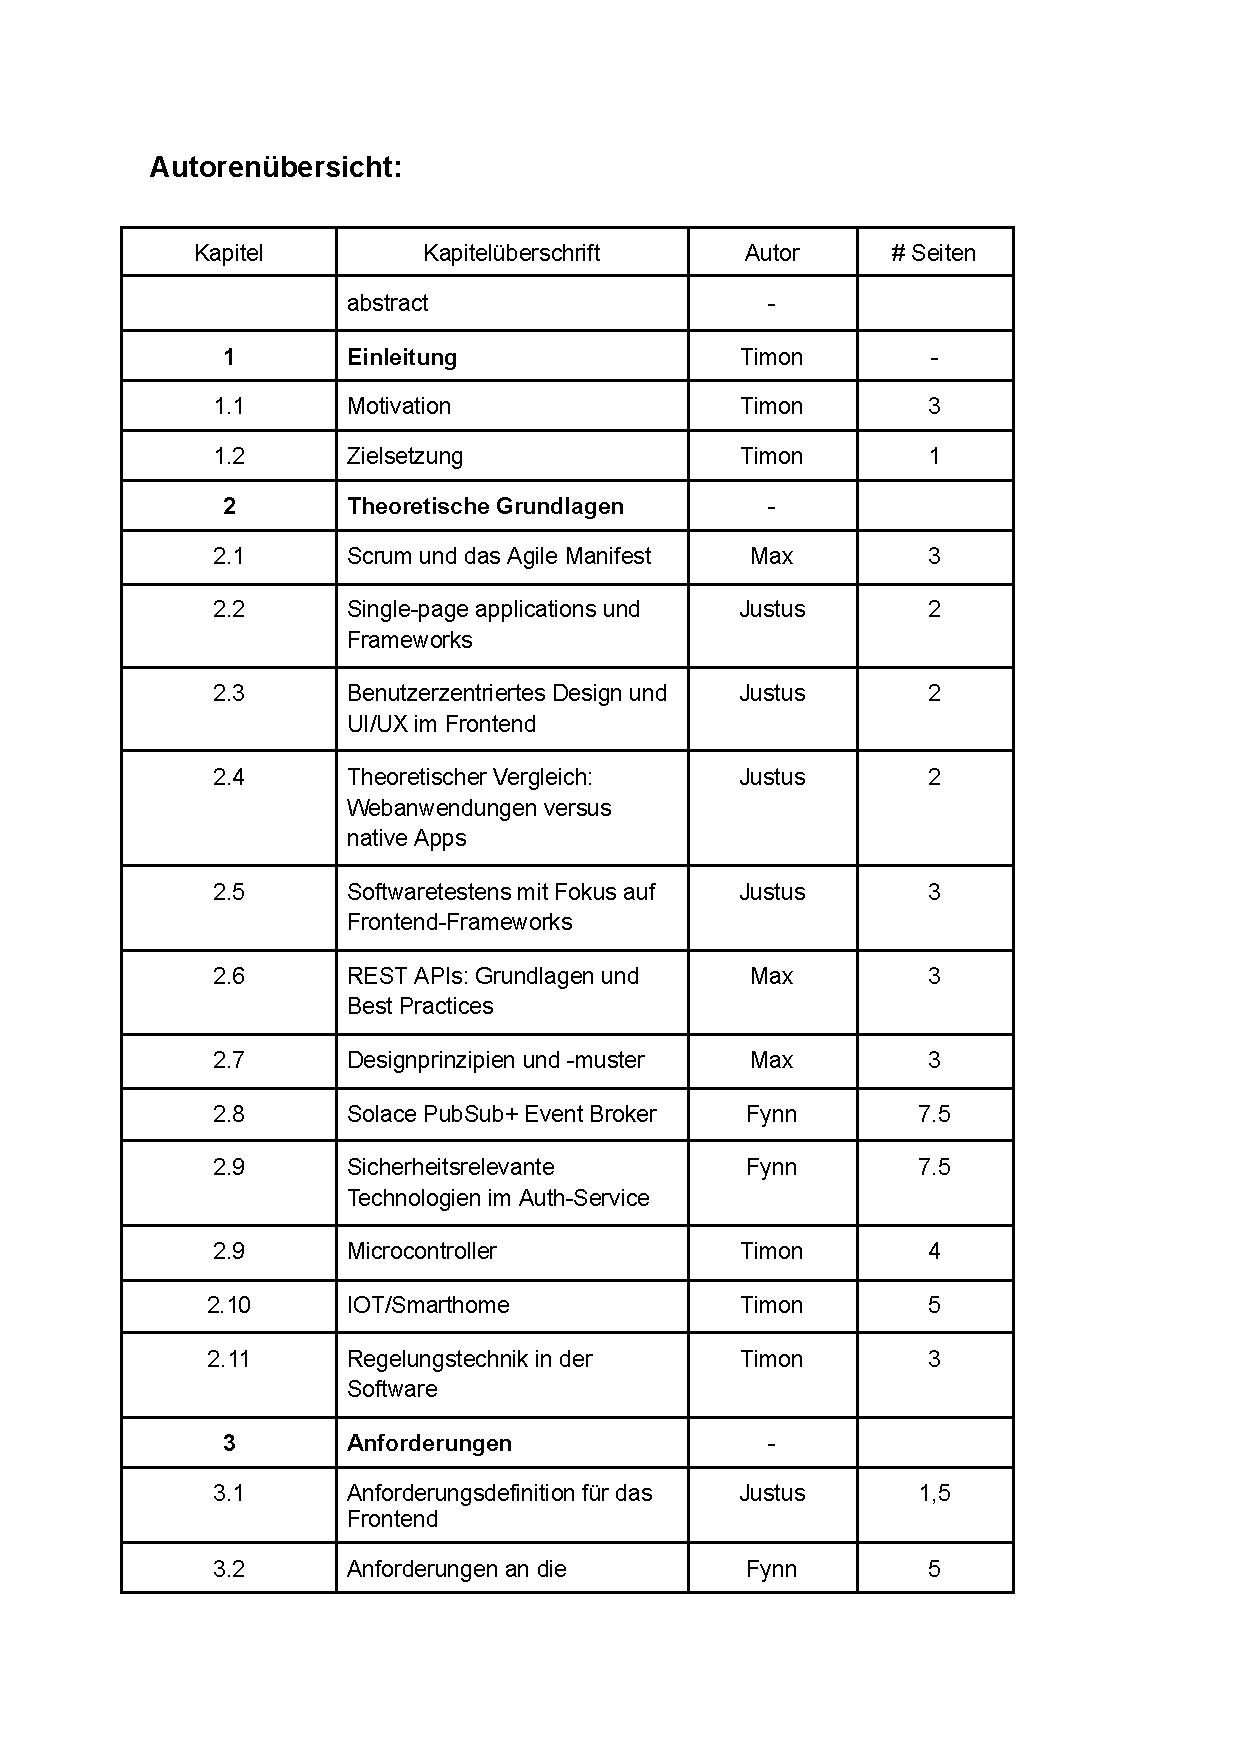
\includepdf[pages=-]{./img/Kapitelautorenschaft.pdf}
	%\fancyhead[R]{ANHANG}

	%\chapter*{Anhang}
	%\addcontentsline{toc}{chapter}{Anhang}

	% Hier Anhänge einfügen:
	%\input{./Anhang/sensorwerte}
	%\input{./Anhang/schaltplan}

\newpage

	
\end{document}
